% Copyright (c) 2020 Carl Martin Ludvig Sinander.

% This program is free software: you can redistribute it and/or modify
% it under the terms of the GNU General Public License as published by
% the Free Software Foundation, either version 3 of the License, or
% (at your option) any later version.

% This program is distributed in the hope that it will be useful,
% but WITHOUT ANY WARRANTY; without even the implied warranty of
% MERCHANTABILITY or FITNESS FOR A PARTICULAR PURPOSE. See the
% GNU General Public License for more details.

% You should have received a copy of the GNU General Public License
% along with this program. If not, see <https://www.gnu.org/licenses/>.

%                                   _     _      
%    _ __  _ __ ___  __ _ _ __ ___ | |__ | | ___ 
%   | '_ \| '__/ _ \/ _` | '_ ` _ \| '_ \| |/ _ \
%   | |_) | | |  __/ (_| | | | | | | |_) | |  __/
%   | .__/|_|  \___|\__,_|_| |_| |_|_.__/|_|\___|
%   |_|                                          


%%% bug catcher
\RequirePackage[l2tabu,orthodox]{nag}

%%% document class
\documentclass[11pt,letterpaper,reqno,oneside]{article}

%%% settings
\input{preamble.tex}

%%% bibliography
\addbibresource{bibl.bib}

%%% externalise TikZ drawings
% \usetikzlibrary{external}
% \tikzexternalize



%______________________________________________________________________________




%    _____ _ _   _      
%   |_   _(_) |_| | ___ 
%     | | | | __| |/ _ \
%     | | | | |_| |  __/
%     |_| |_|\__|_|\___|


\title{\scshape Econometrics II \\
	\vspace{0.5em}
	\large \scshape Taught by Joel Horowitz \\
	\large \scshape Northwestern University, winter 2016
	}

\author{Ludvig Sinander \\ Northwestern University}

\date{\small This version: 12 December 2018}

\makeatletter
	\AtBeginDocument{ \hypersetup{ 
		pdftitle = {Econometrics II}, 
		pdfauthor = {Ludvig Sinander} 
		} }
\makeatother



%______________________________________________________________________________




%    ____                                        _   
%   |  _ \  ___   ___ _   _ _ __ ___   ___ _ __ | |_ 
%   | | | |/ _ \ / __| | | | '_ ` _ \ / _ \ '_ \| __|
%   | |_| | (_) | (__| |_| | | | | | |  __/ | | | |_ 
%   |____/ \___/ \___|\__,_|_| |_| |_|\___|_| |_|\__|


\begin{document}

\maketitle

\noindent
These notes are based on an econometrics course for first-year PhD students taught by Joel Horowitz at Northwestern in winter 2016. The topics are limit theory and the asymptotic properties of extremum estimators.\\

\noindent
I thank Joel for teaching a great class and for agreeing to let me share these notes, and Ahnaf Al Rafi, Bence Bardóczy, Ricardo Dahis, Michael Gmeiner and Joe Long for reporting errors.



\pagebreak
\hspace{1pt}\vfill
\noindent
Copyright \copyright{} 2020 Carl Martin Ludvig Sinander.

\begin{quotation}
\noindent
Permission is granted to copy, distribute and/or modify this document under the terms of the \href{https://www.gnu.org/licenses/fdl}{GNU Free Documentation License}, Version 1.3 or any later version published by the Free Software Foundation; with no Invariant Sections, no Front-Cover Texts, and no Back-Cover Texts. A copy of the license is included in the section entitled `GNU
Free Documentation License'.
\end{quotation}

\noindent
This is a `copyleft' licence.
Visit \href{https://www.gnu.org/licenses/copyleft}{gnu.org/licenses/copyleft} to learn more.



%%%%%%%%%%%%%%%%%%%
%%%%%%%%%%%%%%%%%%%
% Table of contents
\pagebreak
\microtypesetup{protrusion=false}
\tableofcontents
\microtypesetup{protrusion=true}
%%%%%%%%%%%%%%%%%%%
%%%%%%%%%%%%%%%%%%%



\pagebreak
%%%%%%%%%%%%%%%%%%%%%%%%%
%%%%%%%%%%%%%%%%%%%%%%%%%
\section{Outline}
\label{sec:outline}
%%%%%%%%%%%%%%%%%%%%%%%%%
%%%%%%%%%%%%%%%%%%%%%%%%%

%\emph{Covered on 4 Jan 2016.}

Econometrics is about inferring functional relations among variables from data. Schematically, we observe a set of realisations of random vector $(x,y)$, and wish to learn the function $f(\cdot,0)$ that satisfies $y=f(x,u)$ for some unknown random vector $u$.%
	\footnote{It is wlog to say that we want to learn $f(\cdot,0)$. If we want to learn $f(\cdot,\xi)$ for $\xi \neq 0$, just reparameterise as $u' \coloneqq u-\xi$.}
One intuitive way of thinking about this problem is to divide it into two parts: learning the parametric form (`shape') of $f(\cdot,0)$, and learning the values of its parameters. (This intuition underlies parametric methods of estimation. Many nonparametric methods do not divide things up in this way.)

We'll need to sharpen up the question a bit in order to answer it. In general, we cannot learn $f(\cdot,0)$. As we know from Manski's course, the most that we can hope to learn is the joint distribution $\PP(x,y)$ of $(x,y)$. Often, we are interested in some feature of the joint distribution, such as $\PP(y|x)$, $\E(y|x)$ or some quantile of $y$ conditional on $x$. These objects can be thought of as features of the function $f$ when convenient.

A natural approach to estimating $\PP(x,y)$ or $\PP(y|x)$ when the support is finite is to use the empirical distribution. By a law of large numbers, this gives a pointwise consistent estimate.%
	\footnote{In fact, this estimator is uniformly strongly consistent by the Glivenko--Cantelli theorem \parencite[][p. 269]{Billingsley1995}.}
When the support is uncountable, we could of course discretise the outcome space and apply the same reasoning. One drawback to this approach is that we'll often need a fine grid to provide a good approximation, in which case we'll need an astronomical dataset in order to have more than zero or one observation per cell. Another drawback is that we lose the tractability of analysis. (Discrete maths can be ugly.)

Another issue is that on any finite dataset, there is an infinite number of lines that you can fit through the data. In order for a fitted line to approximate the true relationship more and more closely as the sample size increases, we will therefore require some assumptions on the distribution of $(y,x)$. For concreteness, consider the conditional mean function $g(x) \coloneqq \E(y|x)$. In this case, we can estimate $g$ using nonparametric regression provided that $g$ is continuous. We avoid discretisation by taking local averages, using a bandwidth that shrinks as the sample size increases. Continuity guarantees that whatever weighted local average you take (e.g. which kernel you use in kernel regression), the fitted line will get close to $g$ as the sample size gets large. Continuity is often a pretty weak assumption in economics.%
	\footnote{In other fields, discontinuity has to be allowed for explicitly. Joel gave the example of image denoising.}

A fundamental problem with nonparametric estimation techniques is the curse of dimensionality. Roughly speaking, this is that the sample size required to get a given level of estimator precision is exponentially increasing in the dimension of $x$. It can be proved that without stronger assumptions, the curse of dimensionality is unavoidable. Very loosely, the idea is that you're asking a finite dataset to tell you about an infinite-dimensional object.

One way of strengthening the assumptions to avoid the curse of dimensionality is to assume that $g$ belongs to a finite-dimensional family of functions. Schematically, we assume that $g(x) = G(x,\theta)$ where $G$ is a known function and $\theta$ is a finite-dimensional, unknown constant, i.e. a parameter. (In this parametric case, it is often natural to do inference directly on $\theta$ rather than trying to learn $g$ directly.) It turns out (unsurprisingly) that parametrisation defeats the curse of dimensionality. The price we pay for this victory is the need to specify the function $G$. If we misspecify $G$, the math won't break, but the interpretation of results may be way off.

The obvious next conern is the `accuracy' of our estimate of $\theta$ (or $g$). (If we didn't care about accuracy, there would be no reason to use the data!) Since an estimator of $\theta$ is a function of the (random) data, an estimator is a random variable. To characterise accuracy, we have to study this random variable. The problem is that the distribution of an estimator depends on the unknown distribution of $(x,y)$. (If we knew the population distribution, we would once again have no use for a dataset.) Except under very stringent conditions, we cannot consistently estimate (never mind infer with certainty) the distribution of an estimator.

The way we get around this is by using approximations to the distribution of an estimator. If we are to trust these approximations, they must become increasingly good as the data gets increasingly good, in some sense to be made precise. The leading example will be asymptotic approximations, which are approximations that (usually) become increasingly good as the sample size grows. There are many kinds of asymptotic approximation, but the general idea is easily illustrated using the simplest central limit theorem. Suppose that our estimator $\widehat{\theta}$ is an average of $n$ iid random variables (many estimators are), where $n$ is the sample size. Then the central limit theorem says that $n^{1/2} \widehat{\theta}$ converges in distribution to $\mathcal{N}\left(\theta,\sigma^2\right)$, a two-dimensional family of distributions!

Our focus will be on asymptotic theory for parametric estimators. Besides this restriction, our treatment will be general, though common special cases will be mentioned along the way. We'll first cover basic (measure-theoretic) probability theory, then limit theorems. Once the machinery is in place, we will develop the asymptotic theory of extremum estimators.


The course starts off with background probability theory, emphasising concepts required for asymptotic theory. We then state and prove several laws of large numbers and central limit theorems. With the technical machinery in place, we establish the consistency and asymptotic normality of general extremum estimators. We apply these results to maximum likelihood and generalised-method-of-moments estimators, and cover efficiency and specification tests while we're at it. Finally, we study hypothesis testing in the setting of extremum estimation.

The main references for the course are \textcite{Amemiya1985} and \textcite{NeweyMcfadden1994}. These texts (unlike most others in econometrics) raise and address all the important technical issues. Joel will also sometimes to refer \textcite{Rao1973} and \textcite{Serfling1980}, two statistics texts that are worth studying for anyone interested in research in econometric theory. Several other texts that will be mentioned along the way, e.g. \textcite{White2001}.



\pagebreak
%%%%%%%%%%%%%%%%%%%%%%%%%%%%%%%%%%%
%%%%%%%%%%%%%%%%%%%%%%%%%%%%%%%%%%%
\section{Probability theory}
\label{sec:probability}
%%%%%%%%%%%%%%%%%%%%%%%%%%%%%%%%%%%
%%%%%%%%%%%%%%%%%%%%%%%%%%%%%%%%%%%

\emph{%Covered on 6 \& 11 Jan 2016.
Official reading: \textcite[][ch. 2]{Rao1973}.}

This section covers basic (measure-theoretic) probability theory. There is a very large number of good texts on measure and probability theory; Joel mentioned \textcite{KolmogorovFomin1975} in particular.



%%%%%%%%%%%%%%%%%%%%%%%%%%%%%%%%%%%%%%%%%
\subsection{Measurable spaces}
\label{sec:probability:measurable_spaces}
%%%%%%%%%%%%%%%%%%%%%%%%%%%%%%%%%%%%%%%%%

Let $\Omega$ be an arbitrary set. In the context of probability theory, we call $\Omega$ the sample space, and interpret it as the set of all possible states of nature, or outcomes of an experiment.
%
\begin{definition}
	%
	A collection $\mathcal{A}$ of subsets of $\Omega$ is called a $\sigma$-algebra (of subsets of $\Omega$) iff
	%
	\begin{enumerate}

		\item $\Omega \in \mathcal{A}$.

		\item If $A \in \mathcal{A}$ then $A^\compl \in \mathcal{A}$.%
			\footnote{$A^\compl \coloneqq \Omega \backslash A$ denotes the complement of $A$ in $\Omega$.}

		\item If $A_j \in \mathcal{A}$ for each $j \in \N$, then $\Union_{j \in \N} A_j \in \mathcal{A}$.%
			\footnote{$\N = \{1,2,\dots\}$ denotes the natural numbers.}

	\end{enumerate}
	%
\end{definition}



Some additional properties of $\sigma$-algebras are easily derived. For example, if $A_j \in \mathcal{A}$ for each $j \in \N$, then
%
\begin{equation*}
	\Intersect_{j \in \N} A_j
	= \left( \Union_{j \in \N} A_j^\compl \right)^\compl 
	\in \mathcal{A}
\end{equation*}
%
by properties (2) and (3). Another one is $\nullset \in \mathcal{A}$, which follows from (1) and (2).


\begin{definition}
	%
	Let $\Omega$ be an arbitrary set, and let $\mathcal{A}$ be a $\sigma$-algebra of subsets of $\Omega$. We call $(\Omega,\mathcal{A})$ a measurable space. The elements of $\mathcal{A}$ are called the measurable subsets of $\Omega$; subsets of $\Omega$ that are not in $\mathcal{A}$ are called non-measurable.
	%
\end{definition}

The idea is that when we start assigning measure to subsets of $\Omega$, we will only assign measure to the subsets of $\Omega$ that lie in $\mathcal{A}$; this is why we call these subsets measurable. It might seem like we could make our lives easier by choosing $\mathcal{A}=2^\Omega$, the set of all subsets of $\Omega$. We do not do this because for general uncountable $\Omega$, it leads to paradoxes. This will be less of a problem than it may first appear to be because the subsets of $\Omega$ missing from the $\sigma$-algebras we will be working with are very strange sets. But can still give rise to difficulties: measurability problems arise fairly frequently in econometric and economic theory.

In the context of probability theory, we sometimes call the measurable sets `events', and interpret them as `something that happens'. To illustrate, suppose we draw one coloured ball from an urn, formalised by the measurable space $\bigl( \{\text{red},\text{blue},\text{green}\}, 2^{\{\text{red},\text{blue},\text{green}\}} \bigr)$. In ordinary language, one `event' I might describe is `I pick a red or a blue ball'. In the formalism, this corresponds to the event (measurable set) $\{\text{red},\text{blue}\}$.


We might wonder how to choose our $\sigma$-algebra. An important criterion is that our $\sigma$-algebra contain enough subsets of $\Omega$ to allow us to study convergence (of measures, of measurable functions and of integrals). Convergence is a topological notion, so let's equip $\Omega$ with a topology. In order to obtain convergence results, we will need the $\sigma$-algebra to contain enough topologically interesting subsets of $\Omega$; at the very least, it should contain all of the open subsets of $\Omega$. It turns out that this minimal requirement is enough for most purposes, leading to the following definition.

\begin{definition}
	%
	Let $(\Omega,\mathcal{T})$ be a topological space. The Borel $\sigma$-algebra of subsets of $\Omega$ (relative to topology $\mathcal{T}$) is the smallest $\sigma$-algebra of subsets of $\Omega$ that contains $\mathcal{T}$ (all of the open sets). When $\Omega$ and its topology are clear from the context, we'll write $\mathcal{B}$ for the Borel $\sigma$-algebra.
	%
\end{definition}

More broadly, we will sometimes be interested in a certain collection $\mathcal{X}$ of subsets of $\Omega$. In order to say measure-theoretic things about them, we need them to be measurable! To this end, we write $\sigma(\mathcal{X})$ for the smallest $\sigma$-algebra of subsets of $\Omega$ that contains $\mathcal{X}$; $\sigma(\mathcal{X})$ is called the $\sigma$-algebra generated by $\mathcal{X}$. Note that for a topological space $(\Omega,\mathcal{T})$, the $\sigma$-algebra $\sigma(\mathcal{T})$ generated by the open sets is exactly the Borel $\sigma$-algebra.



%%%%%%%%%%%%%%%%%%%%%%%%%%%%%%%%
\subsection{Measures}
\label{sec:probability:measures}
%%%%%%%%%%%%%%%%%%%%%%%%%%%%%%%%

Let $\widebar{\R} = \R \union \{ -\infty, \infty \}$ be the extended real line.

\begin{definition}
	%
	Given a measurable space $(\Omega,\mathcal{A})$, a function $\mu : \mathcal{A} \to \widebar{\R}$ is a measure iff
	%
	\begin{enumerate}

		\item $\mu(A) \geq 0$ for each $A \in \mathcal{A}$.

		\item If $A_j \in \mathcal{A}$ for each $j \in \N$ are disjoint, then
		%
		\begin{equation*}
			\mu\left( \Union_{j \in \N} A_j \right) = \sum_{j \in \N} \mu(A_j) .
		\end{equation*}
		%
		(This property is called countable additivity.)

	\end{enumerate}
	%
	If in addition $\mu(\Omega) = 1$, then $\mu$ is a probability measure. We often use $\PP$ to denote a probability measure.
	%
\end{definition}

\begin{definition}
	%
	Let $(\Omega,\mathcal{A})$ be a measurable space, and let $\mu$ be a measure on $(\Omega,\mathcal{A})$. We call $(\Omega,\mathcal{A},\mu)$ a measure space. If $\mu$ is a probability measure, we call it a probability (measure) space.
	%
\end{definition}


%George David Birkhoff (1884--1944) showed that if you want the probability of a point to be zero, then you cannot construct a $\sigma$-finite measure on an uncountable set. (In particular, you cannot construct a probability measure.) The proof makes use of the axiom of choice and the continuum hypothesis.


%Some obvious consequences of our definitions are as follows. Since $1 = \PP(\Omega) = \PP(A) + \PP\left( A^\compl \right) \geq 0$, $\PP(A) \leq 1$ for any $A \in \mathcal{A}$.

\begin{example}[Lebesgue measure]
	%
	Let $\Omega = [0,1]$, let $\mathcal{B}$ be the Borel $\sigma$-algebra, and let $\mathcal{I}$ be the intervals of $[0,1]$. Let $\lambda : \mathcal{I} \to \widebar{\R}$ be the probability measure on $(\R,\mathcal{I})$ with the property that the value of an interval is its length, e.g. $\lambda((a,b]) = b-a$. It turns out that there's a unique extension of $\lambda$ to the rest of $\mathcal{B}$ that respects the measure axioms.%
		\footnote{This follows from an extension theorem. Extension theorems provide conditions for the existence, and sometimes uniqueness, of an extension of a measure from a small set (e.g. the intervals) to a larger set (e.g. the Borel $\sigma$-algebra).}$^,$%
		\footnote{Actually, there's a unique extension to $([0,1],\mathcal{L})$, where $\mathcal{L}$ is a larger $\sigma$-algebra called the Lebesgue-measurable sets.}
	This measure is called Lebesgue measure on $([0,1],\mathcal{B})$. We can similarly define Lebesgue measure on other subsets of $\R^n$ for $n \in \N$.

	One property of this measure is that any countable set has Lebesgue measure zero. To show this, take a collection of distinct points $x_j \in [0,1]$ for each $j \in \N$. Since $\lambda(\{x_j\})=0$ for each $j \in \N$ (each is an interval of length zero), countable additivity yields
	%
	\begin{equation*}
		\lambda\left( \Union_{j \in \N} \{x_j\} \right) 
		= \sum_{j \in \N} \lambda(\{x_j\}) 
		= \sum_{j \in \N} 0 
		= 0 .
	\end{equation*}
	%
	It follows, for example, that $\lambda( \Q \intersect [0,1] ) = 0$.%
		\footnote{$\Q$ denotes the rational numbers.}
	%
\end{example}

Let $(\Omega,\mathcal{A},\mu)$ be a measure space, and consider some property $P$ that does or does not hold at each $\omega \in \Omega$. We say that property $P$ holds $\mu$-almost everywhere ($\mu$-a.e.) on $\Omega$ iff it holds everywhere on $\Omega$ except possibly on a set of $\mu$-measure zero.%
	\footnote{That is, there is some $A \in \mathcal{A}$ such that $P$ holds at every $\omega \in A$ and $\mu(A^\compl)=0$.}
For example, a standard real analysis result states that any monotone function $f : \R \to \R$ is continuous $\lambda$-a.e., where $\lambda$ is Lebesgue measure on $(\R,\mathcal{B})$. When $\mu$ is a probability measure and $P$ holds $\mu$-a.e., we usually say that $P$ holds $\mu$-almost surely ($\mu$-a.s.) or that $P$ holds with probability 1. More generally, `$\mu$-almost' is used flexibly as an adverb, e.g. `$\mu$-almost all' or `$\mu$-almost every'.



%%%%%%%%%%%%%%%%%%%%%%%%%%%%%%%%%%%%%%%%%%%%
\subsection{Measurable functions}
\label{sec:probability:measurable_functions}
%%%%%%%%%%%%%%%%%%%%%%%%%%%%%%%%%%%%%%%%%%%%

For a function $f : F \to G$ and a subset $B \subseteq G$, write
%
\begin{equation*}
	f^{-1}(B)
	\coloneqq \left\{ x \in F : f(x) \in B \right\} .
\end{equation*}
%
(This is standard notation, but worth writing down just in case.)

\begin{definition}
	%
	Let $(F,\mathcal{F})$ and $(G,\mathcal{G})$ be measurable spaces. Then $f : F \to G$ is $\mathcal{F}$/$\mathcal{G}$-measurable iff for any $B \in \mathcal{G}$, $f^{-1}(B) \in \mathcal{F}$. When one or both $\sigma$-algebras are clear from the context, we sometimes shorten this to `$\mathcal{F}$-measurable' or simply `measurable'.%
		\footnote{For the special case of functions $f : \R^n \to \R$ with the Borel $\sigma$-algebras $\mathcal{B}^n$ and $\mathcal{B}$, $\mathcal{B}^n/\mathcal{B}$-measurability is sometimes called Borel-measurability.}
	%
\end{definition}

In words, measurable sets of values are generated by measurable sets of arguments. This is very similiar to the definition of continuity from topology, where a function is continuous iff open sets of values are generated by open sets of arguments. Notice that the measurability of a function depends only on the measurable spaces; it has nothing to do with measures defined on those spaces.%
	\footnote{Some confusing (in my view) terminology was used at this point in the lecture. Consider two measurable spaces $(F,\mathcal{F})$ and $(G,\mathcal{G})$, a measure $\mu$ on $(F,\mathcal{F})$, and a function $f : F \to G$. Above, I defined the property of $\mathcal{F}$/$\mathcal{G}$-measurability of $f$. Joel called this same property $\mu$-measurability of $f$. But as I pointed out, the measure $\mu$ has nothing to do with it!}

Measurability is needed because the whole point of measure theory is to assign measure to things. If a function maps from one measurable space to another, we'd like to be able to say that the measure of a measurable set of values in $G$ of the function is equal to the measure of the set of arguments in $F$ that generate those values. But if our function is not measurable, then there will be sets of values in $G$ that are counted as measurable according to $(G,\mathcal{G})$, but which are generated by a set of arguments in $F$ that is not measurable according to $(F,\mathcal{F})$.


A special case of interest is where $(F,\mathcal{F}) = (\Omega,\mathcal{A})$ is an arbitrary measurable space and $(G,\mathcal{G}) = \bigl(\R^k,\mathcal{B}\bigr)$ where $\mathcal{B}$ is the Borel $\sigma$-algebra on $\R^k$. It turns out that in this case, a function $f : \Omega \to \R^k$ is measurable iff
%
\begin{equation*}
	\{ \omega \in \Omega : f(\omega) \leq z \} \in \mathcal{A}
	\quad \text{for each $z \in \R^k$} .
\end{equation*}


We can now define random elements, which are principal characters in the sequel.
%
\begin{definition}
	%
	Let $(\Omega,\mathcal{A},\PP)$ be a probability space, and let $(S,\mathcal{S})$ be a measurable space. A random element of $(S,\mathcal{S})$ defined on $(\Omega,\mathcal{A},\PP)$ is an $\mathcal{A}/\mathcal{S}$-measurable function $X : \Omega \to S$.
	%
\end{definition}
%
The set $S$ in which a random element takes values can be entirely arbitrary; it need not be a topological or metric space, for example. But often, $S$ will be a metric space. In this case, we will sometimes abuse terminology by saying `random element of $(S,\rho)$ (defined on $(\Omega,\mathcal{A},\PP)$)', on the understanding that $S$ is equipped with a $\sigma$-algebra, usually the Borel $\sigma$-algebra generated by the topology induced by the metric $\rho$.

\begin{definition}
	%
	A random variable is a random element of $\left(\R,\mathcal{B}\right)$.
	A random $n$-vector is a random element of $\left(\R^n,\mathcal{B}\right)$.
	A random $n \times m$ matrix is a random element of $\left(\R^{n \times m},\mathcal{B}\right)$.
	%
\end{definition}


For a random element $X : \Omega \to S$ and a measurable subset $B$ of $S$, $X^{-1}(B)$ is the set of states of the world $\omega \in \Omega$ at which $X(\omega)$ lies in $B$. We know that $X^{-1}(B) \in \mathcal{A}$ since $X$ is a measurable function. But $\mathcal{A}$ may contain lots of other events that do not correspond to $X^{-1}(B)$ for some $B \in \mathcal{S}$. These other events are not interesting for the study of $X$, so we sometimes wish to use smaller the $\sigma$-algebra that contains all the sets of interest for $X$ but no others. In our previous jargon, what we want is the $\sigma$-algebra generated by the interesting sets, viz. $\sigma\bigl( \left\{ X^{-1}(B) \right\}_{ B \in \mathcal{S} } \bigr)$. The name of this object is often shortened to `the $\sigma$-algebra generated by $X$', or $\sigma(X)$.



\begin{definition}
	%
	Let $X$ be a random element of $(S,\mathcal{S})$ defined on $(\Omega,\mathcal{A},\PP)$. The law (or distribution) of $X$ is the function $\mathcal{L}_X : \mathcal{S} \to \R$ given by $\mathcal{L}_X(B) \coloneqq \PP( X \in B )$ for each $B \in \mathcal{S}$.%
		\footnote{$\PP( X \in B )$ is shorthand for $\PP( \{ \omega \in \Omega : X(\omega) \in B \} )$.}
	%
\end{definition}

If we are interested only in the behaviour of the random element $X$, then all of the information we need is contained in its law $\mathcal{L}_X$. It does not matter what probability space it is defined on! In fact, $(S,\mathcal{S},\mathcal{L}_X)$ is itself a probability space, and the random element $Y$ defined by $Y(s) \coloneqq s$ for each $s \in S$ on this probability space has law $\mathcal{L}_Y = \mathcal{L}_X$.


When $X$ is a random vector, there's is an alternative (more tractable) object that fully describes the behaviour of $X$: the CDF.
%
\begin{definition}
	%
	Let $X$ be a random vector. The cumulative distribution function (CDF) of $X$ is $F_X : \R^n \to [0,1]$ defined by
	%
	\begin{equation*}
		F_X(x_1,\dots,x_n) \coloneqq 
		\mathcal{L}_X( (-\infty,x_1] \times \cdots \times (-\infty,x_n] )
	\end{equation*}
	%
	for each $(x_1,\dots,x_n) \in \R^n$.
	%
\end{definition}
%
It is intuitive (but not quite obvious, I think) that $F_X$ fully characterises the law of a random vector. Precisely stated: for random vectors $X$ and $Y$, $\mathcal{L}_X = \mathcal{L}_Y$ (setwise) iff $F_X = F_Y$ (pointwise). See \textcite[][Proposition 6.0.2]{Rosenthal2006} for a (very easy) proof.


Some properties of CDFs are that they are right-continuous, nondecreasing, and satisfy $\lim_{x\to -\infty} F(x) = 0$ and $\lim_{x\to\infty} F(x) = 1$.
(For $n=1$, we have a converse: any function $F : \R \to [0,1]$ with these four properties is the CDF of some random vector on some probability space.)
%Another property: any discontinuity in a CDF must be a jump discontinuity (because CDFs are monotone).

We can also define random elements $X : \Omega \to \widebar{\R}^n$ that are like random vectors but can take infinite values. If $\mathcal{L}_X\left(\R^n\right)<1$, then the distribution $\mathcal{L}_X$ of $X$ is said to be defective. Conversely, if $\mathcal{L}_X\left(\R^n\right)=1$ then the distribution is called proper. Though we rarely \emph{want} to work with random vectors that take infinite values with positive probability, we sometimes 
obtain a random vector with a defective distribution as the limit of a sequence of random vectors with proper distributions.



%%%%%%%%%%%%%%%%%%%%%%%%%%%%%%%%%%%%
\subsection{Independence}
\label{sec:probability:independence}
%%%%%%%%%%%%%%%%%%%%%%%%%%%%%%%%%%%%

Probability theory is basically measure theory plus independence. This will become increasingly clear: all of the interesting theorems that we will state specifically for probability measures (rather than general measures) assume (some weakened form of) independence.
%
\begin{definition}
	%
	For a probability space $\left(\Omega,\mathcal{A},\PP\right)$, events $A,B \in \mathcal{A}$ are independent iff $\PP( A \intersect B ) = \PP(A) \PP(B)$.
	%
\end{definition}

Sometimes, we wish to impose independence for two whole classes of events. Call $\mathcal{F}$ a sub-$\sigma$-algebra of the $\sigma$-algebra $\mathcal{A}$ iff it is a $\sigma$-algebra of subsets of $\Omega$ and $\mathcal{F} \subseteq \mathcal{A}$.
%
\begin{definition}
	%
	For a probability space $\left(\Omega,\mathcal{A},\PP\right)$, sub-$\sigma$-algebras $\mathcal{F}$ and $\mathcal{G}$ of $\mathcal{A}$ are independent iff $\PP( F \intersect G ) = \PP(F) \PP(G)$ for every $F \in \mathcal{F}$ and $G \in \mathcal{G}$.
	%
\end{definition}


Fix a probability space $\left(\Omega,\mathcal{A},\PP\right)$ and a measurable space $(S,\mathcal{S})$. Two random elements $X$ and $Y$ of $(S,\mathcal{S})$ are called independent iff their generated $\sigma$-algebras $\sigma(X)$ and $\sigma(Y)$ are independent. This just means that
%
\begin{equation*}
	\PP( X \in B_X, Y \in B_Y ) = \PP( X \in B_X ) \PP( Y \in B_Y )
\end{equation*}
%
for any measurable subsets $B_X$ and $B_Y$ of $S$. (So for random vectors, $B_X$ and $B_Y$ are any Borel sets.)



%%%%%%%%%%%%%%%%%%%%%%%%%%%%%%%%%%%%%%%%%
\subsection{The Lebesgue integral}
\label{sec:probability:Lebesgue_integral}
%%%%%%%%%%%%%%%%%%%%%%%%%%%%%%%%%%%%%%%%%

A problem with the Riemann integral is that many interesting functions are not Riemann-integrable. This defect is addressed by the Lebesgue integral.
When $\Omega = \R$, the standard Lebesgue integral of a measurable function $f : \Omega \to \R$ is written $\int_\Omega f \dd \lambda$, where $\lambda$ is Lebesgue measure on $\R$. To integrate over a measurable subset $S \subseteq \R$, define
%
\begin{equation*}
	\int_S f \dd \lambda \coloneqq \int_\Omega f \1_S \dd \lambda
\end{equation*}
%
where $\1_S$ is the indicator function for $S$.%
	\footnote{I.e. $\1_S(\omega)=1$ iff $\omega \in S$, $0$ otherwise.}
The Lebesgue integral does not exist for every measurable function:
a boundedness condition is also needed to avoid the undefined expression $\infty-\infty$.

A measurable function is called Lebesgue-integrable iff its integral exists and is finite.%
	\footnote{A necessary and sufficient condition for a measurable function $f$ to be integrable is that $\int_\Omega \abs{f} \dd \lambda < \infty$.}
Any Riemann-integrable function is also Lebesgue-integrable, and in such cases the two integrals coincide. But many functions are Lebesgue- but not Riemann-integrable.%
	\footnote{For example, consider the function $f : \R \to \R$ such that $f(x) = \1( x \notin \Q )$. This function is not Riemann-integrable, but it is Lebesgue-integrable, with $\int_\R f \dd \lambda = 1$ as we would hope. More generally, there are certain kinds of discontinuity that Lebesgue integration can handle but Riemann integration cannot.}$^,$%
	\footnote{In terms of how they are constructed, the difference between the two integrals is that while the Riemann integral considers the limit of a sequence of approximations to the `area under $f$' constructed by discretising the $x$ axis, the Lebesgue integral considers approximations constructed by discretising the $y$ axis.}

In constructing the Lebesgue integral, it quickly becomes apparent that we can replace the Lebesgue measure $\lambda$ with whatever measure $\mu$ we like, leading to the generalised Lebesgue integral $\int_S f \dd \mu$.
Of course, the conditions under which $f$ is integrable depend on what measure we're integrating with respect to. If $\int_S f \dd \mu$ exists, we say that $f$ is $\mu$-integrable.

Importantly, the Lebesgue integral may defined for measurable functions $f : \Omega \to \R$ on \emph{any} measurable space $\left( \Omega, \mathcal{A} \right)$, not just (say) $\R$ or $\R^n$.
This provides a powerful generalisation of Riemann integration; for example, we can integrate over functional spaces.

Now consider the case in which $\mu$ is a probability measure on a measurable space $(\Omega,\mathcal{A})$, so that the measurable function $f$ is a random variable. Let's use the more familiar notation of $\PP$ for the measure and $X$ for the random variable. In this setting, the Lebesgue integral $\int_\Omega X \dd \PP$ is also called the expected value of $X$ (or the expected value of the distribution $\mathcal{L}_X$).
Since not all measurable functions admit an integral, there are random variables whose expectation is undefined. (One example is a Cauchy-distributed random variable.)
Even when the expectation exists, it may be infinite.

There are various kinds of notation for the expected value, including:
%
\begin{equation*}
	\E( X ) 
	= \int_\Omega X \dd\PP
	= \int_\Omega X(\omega) \dd\PP(\omega)
	= \int_\Omega X(\omega) \PP(\dd\omega) .
\end{equation*}
%
Sometimes, we wish to work with $\mathcal{L}_X$ rather than $X$ and $\PP$; in these cases we sometimes write $\E(\mathcal{L}_X)$ (confusingly!). It is simple to show (e.g. \textcite[][Theorem 6.1.1]{Rosenthal2006}) that the expected value can be written as an integral with respect to the law of $X$,%
	\footnote{Recall that $(\R,\mathcal{B},\mathcal{L}_X)$ is a probability space.}
so that
%
\begin{equation*}
	\E(X)
	= \E( \mathcal{L}_X )
	= \int_\R x \dd \mathcal{L}_X(x) 
	= \int_\R x \mathcal{L}_X(\dd x) . 
\end{equation*}


Finally, we can rewrite the integral in terms of the CDF $F_X$ rather than the law $\mathcal{L}_X$. This is unsurprising in view of the fact that CDFs coincide iff the laws do. The integral w.r.t. a CDF is called a Stieltjes integral, and can be written in various ways:
%
\begin{equation*}
	\E( X )
	= \int_\R x \dd F_X(x) 
	= \int_\R x F_X(\dd x) . 
\end{equation*}
%
The Stieltjes integral coincides with the Lebesgue integral, but is defined differently (in terms of the CDF).

Let $X$ be a random variable; then $X^n$ for $n \in \N$ is also a random variable (easy proof). $\E\left( X^n \right)$ is called the $n$th moment of $X$, and $\E\left( (X-\E(X))^n \right)$ is called the $n$th central moment. (Of course, a given moment of $X$ need not exist or be finite.) The second central moment is called the variance of $X$, denoted $\Var(X)$.

While we're at it, here are two related concepts. Let $X$ and $Y$ be random variables. Their covariance is
%
\begin{equation*}
	\Cov(X,Y) \coloneqq \E\left( [X-\E(X)] [Y-\E(Y)] \right) ,
\end{equation*}
%
and their correlation is
%
\begin{equation*}
	\Corr(X,Y) \coloneqq \frac{ \Cov(X,Y) }{ \sqrt{\Var(X)} \sqrt{\Var(Y)} } .
\end{equation*}
%
There are a lot of algebraic shortcuts involving variances, covariances and correlations that are hopefully familiar from undergrad. I won't list them here, but I will make use of them!



%%%%%%%%%%%%%%%%%%%%%%%%%%%%%%%%%%%%%%%%%%%
\subsection{The Radon--Nikod\'{y}m theorem}
\label{sec:probability:Radon-Nikodym}
%%%%%%%%%%%%%%%%%%%%%%%%%%%%%%%%%%%%%%%%%%%

The Radon--Nikod\'{y}m theorem gives conditions under which a measure can be represented as a Lebesgue integral w.r.t. another measure. In particular, given measures $\mu$ and $\nu$ on a measurable space $(\Omega,\mathcal{A})$, we're interested in representations of the form
%
\begin{equation}
	\nu(A) = \int_A f \dd \mu \quad\text{for each $A \in \mathcal{A}$}
	\label{eq:Radon-Nikodym_representation}
\end{equation}
%
for some nonnegative, $\mu$-integrable (hence $\mathcal{A}/\mathcal{B}$-measurable) function $f : \Omega \to \R$.

The following concept will turn out to be the key.
%
\begin{definition}
	%
	Let $\mu$ and $\nu$ be measures defined on a measurable space $(\Omega,\mathcal{A})$. We say that $\mu$ dominates $\nu$, written $\mu \gg \nu$, iff for any $A \in \mathcal{A}$, $\mu(A)=0$ implies $\nu(A)=0$. We also sometimes say that $\nu$ is absolutely continuous w.r.t. $\mu$.%
		\footnote{There's some unhelpful confusion of terminology here. Most authors (e.g. \textcite{KolmogorovFomin1975} and \textcite{Billingsley1995}) use `absolutely continuous' synonymously with `dominates', as in my definition. But \textcite[][p. 143]{Rosenthal2006} defines `$\nu$ absolutely continuous w.r.t. $\mu$' to mean that there exists a nonnegative $f$ such that representation \eqref{eq:Radon-Nikodym_representation} holds. By the Radon--Nikod\'{y}m theorem, the two turn out to be equivalent for $\sigma$-finite measures, but they are still distinct properties that should have distinct names.}
	%
\end{definition}


Suppose that the representation is possible: there is a nonnegative $f$ such that \eqref{eq:Radon-Nikodym_representation} holds. Then if $\mu(A)=0$ for some $A \in \mathcal{A}$, it follows that
%
\begin{equation*}
	\nu(A) 
	= \int_A f(\omega) \mu( \dd \omega )
	= \int_\Omega f(\omega) \1_A(\omega) \mu( \dd \omega )
	= 0
\end{equation*}
%
since $\1_A(\omega)=0$ for all $\omega \in \Omega$ outside a set of $\mu$-measure zero (viz. the set $A$). So we've learned that if \eqref{eq:Radon-Nikodym_representation} holds, then $\mu \gg \nu$. The Radon--Nikod\'{y}m theorem is the (far less obvious) converse to this result: if $\mu \gg \nu$, then there exists a nonnegative $f$ such that \eqref{eq:Radon-Nikodym_representation} holds. Actually, there's a caveat: in order for the converse to hold, both measures must be $\sigma$-finite.

In words, a measure defined on $(\Omega,\mathcal{A})$ is $\sigma$-finite iff there is a countable, measurable cover of $\Omega$ such that every piece of the cover is assigned finite measure. It should be obvious that every probability measure is $\sigma$-finite. For reference, here's a schematic definition:
%
\begin{definition}
	%
	Let $(\Omega,\mathcal{A},\mu)$ be a measure space. The measure $\mu$ is $\sigma$-finite iff there is a countable collection $\{ A_j \}_{j \in \N}$ of subsets of $\Omega$ such that

	\begin{enumerate}

		\item $A_j \in \mathcal{A}$ for each $j \in \N$

		\item $\Union_{j \in \N} A_j = \Omega$

		\item $\mu(A_j)<\infty$ for each $j \in \N$.

	\end{enumerate}
	%
\end{definition}


With definitions in place, we're ready to state the theorem.

\begin{theorem}[Radon--Nikod\'{y}m]
	%
	Let $\mu$ and $\nu$ be $\sigma$-finite measures on some measurable space $(\Omega,\mathcal{A})$, and suppose that $\mu \gg \nu$. Then there is a nonnegative, $\mu$-integrable function $f$ such that $\nu(A) = \int_A f \dd \mu$ for each $A \in \mathcal{A}$.
	%
\end{theorem}

$f$ in the theorem is usually called the density of $\nu$ with respect to $\mu$. (The densities familiar from undergrad are densities w.r.t. Lebesgue measure $\lambda$.) It is also called a Radon--Nikod\'{y}m derivative, denoted $\dd \nu / \dd \mu$. This name is obviously motivated by the fact that
%
\begin{equation*}
	\nu(A) = \int_A \frac{\dd \nu}{\dd \mu} \dd \mu 
	\quad\forall A \in \mathcal{A} ,
\end{equation*}
%
an expression analogous to the fundamental theorem of calculus for ordinary derivatives and the Riemann integral.%
	\footnote{There are other properties which Radon--Nikod\'{y}m derivatives share with ordinary derviatives. One of these is the chain rule: for $\sigma$-finite measures $\nu \ll \mu \ll \tau$ on some measurable space, we have $\tfrac{\dd \nu}{\dd \tau} = \tfrac{\dd \nu}{\dd \mu} \tfrac{\dd \mu}{\dd \tau}$.}


Another property of representation \eqref{eq:Radon-Nikodym_representation} is that the density $f$ is unique up to sets of measure zero: if $f$ and $g$ are both densities of $\nu$ w.r.t. $\mu$ then $\mu( f \neq g ) = 0$.%
	\footnote{That is, $\mu( \{ \omega \in \Omega : f(\omega) \neq g(\omega) \} ) = 0$.}
This is a corollary to a basic property of the Lebesgue integral; a proof can be found in \textcite[][Theorem 16.10]{Billingsley1995}.


\begin{example}[density w.r.t. counting measure]
	%
	As already mentioned, the probability density functions familiar from undergrad are Radon--Nikod\'{y}m derivatives w.r.t. Lebesgue measure. In this example, we'll see that probability \emph{mass} functions (for discrete random variables) are in fact Radon--Nikod\'{y}m derivatives w.r.t. a measure called counting measure.

	Let $(\N,\mathcal{A})$ be a measurable space,%
		\footnote{Recall that $\N=\{1,2,\dots\}$.}
	and let $\PP$ be a probability measure on it. Let $c : \mathcal{A} \to \widebar{\R}$ be defined by $c(A) \coloneqq \abs{A}$ for $A \in \mathcal{A}$.%
		\footnote{$\abs{A}$ denotes the number of elements in the set $A$. For $A$ infinite, $\abs{A}=\infty$; moreover $\abs{\varnothing}=0$.}
	$c$ is obviously a $\sigma$-finite measure on $(\N,\mathcal{A})$; it is called counting measure. Perhaps unsurprisingly, integration w.r.t. counting measure is equivalent to summation: formally, for any $c$-integrable (and measurable) function $f : \N \to \R$,
	%
	\begin{equation*}
		\int_A f \dd c 
		= \sum_{n \in A} f(n) 
		\quad\text{for every $A \in \mathcal{A}$} .
	\end{equation*}
	%
	(If you know how the Lebesgue integral is defined, then this should be trivial.)

	Now let's apply the Radon--Nikod\'{y}m theorem to the $\sigma$-finite measures $\PP$ and $c$. The only set to which $c$ assigns measure zero is $\varnothing$, and $\PP(\varnothing)=0$; hence $\PP \ll c$. So by the Radon--Nikod\'{y}m theorem, there is nonnegative and $c$-integrable function $f : \N \to \R$ such that
	%
	\begin{equation*}
		\PP(A)
		= \int_A f \dd c
		= \sum_{n \in A} f(n)
		\quad\text{for every $A \in \mathcal{A}$} .
	\end{equation*}
	%
	Moreover, $f$ is unique: we already knew it to be unique up to sets of $c$-measure zero, but the only set of $c$-measure zero is $\varnothing$.

	Let's suppose our $\sigma$-algebra is rich enough that it contains all the singletons: $\{ n \} \in \mathcal{A}$ for each $n$. (Using such a rich $\sigma$-algebra would cause problems on an uncountable sample space, but it's fine here since $\N$ is countable.) Then for each $n \in \N$ we have $\PP(\{n\}) = f(n)$, showing that $f$ is the probability mass function.%
		\footnote{The Radon--Nikod\'{y}m theorem doesn't tell us what the function $f$ is, only that it exists. Characterising $f$ will generally require an argument specific to the measure space at hand.}
	%
\end{example}


The Radon--Nikod\'{y}m theorem turns out to have various uses. It is used to establish the existence of useful constructs such as conditional probabilities and conditional expectations (see below). In estimation, if the data are distributed according to $\nu_\theta$ for some parameter $\theta$, then a clever choice of $\mu$ can give us a convenient likelihood function $\mathcal{L}(\theta) \coloneqq \dd \nu_\theta / \dd \mu$.



%%%%%%%%%%%%%%%%%%%%%%%%%%%%%%%%%%%%%%%%%%%%%%%
\subsection{Conditional probability}
\label{sec:probability:conditional_probability}
%%%%%%%%%%%%%%%%%%%%%%%%%%%%%%%%%%%%%%%%%%%%%%%

\emph{This section may be hard to follow. I recommend \textcite[][sec. 33]{Billingsley1995}.}

Consider two events $A$ and $G$ of a probability space $(\Omega,\mathcal{A},\PP)$. Imagine that we learn that event $G$ obtains, and would like to revise the probability of event $A$ in light of this information. (This scenario is obviously ubiquitous in economics and econometrics.) How do we formalise this?

When $\PP(G)>0$, the answer is intuitive and easy: we say that the conditional probability is $\PP(A \intersect G) / \PP(G)$. (Draw a Venn diagram.) The problem is that we (very) often wish to condition on a probability-zero event, i.e. $\PP(G)=0$. (For example, the realisation of a normally distributed signal.) The ratio formula does not apply in this case, so a subtler construction is called for.

To build some intuition, consider a finite probability space $\left(\Omega,2^\Omega,\PP\right)$ in which $\PP(\{\omega\})>0$ $\forall \omega \in \Omega$. Let $\Q(A|G) \coloneqq \PP(A \intersect G) / \PP(G)$ be the `ordinary' probability of $A$ conditional on $G$. Notice that $\Q(A|\{\omega\}) = \1( \omega \in A )$. It follows that for events $A$ and $G$,
%
\begin{multline*}
	\PP(A \intersect G)
	= \sum_{\omega \in A \intersect G} \PP(\{\omega\})
	= \sum_{\omega \in G} \1( \omega \in A ) \PP(\{\omega\})
	\\
	= \sum_{\omega \in G} \Q( A | \{\omega\} ) \PP(\{\omega\}) 
	= \int_G \Q( A | \{\omega\} ) \PP(\dd\omega) .
\end{multline*}
%
(The Lebesgue integral is used because unlike the sum, it remains defined when we move to uncountable probability spaces.) We'd like our definition of conditional probability to respect $\PP(A \intersect G) = \int_G \Q( A | \{\omega\} ) \PP(\dd\omega)$. Since this property does not involve division by $\PP(G)$, we can require it to hold even when $\PP(G)=0$.

We require an additional bit of machinery. Recall that $\mathcal{A}$ is a $\sigma$-algebra of subsets of $\Omega$, we call $\mathcal{G}$ a sub-$\sigma$-algebra of $\mathcal{A}$ iff $\mathcal{G}$ is a $\sigma$-algebra and $\mathcal{G} \subseteq \mathcal{A}$. Since $\mathcal{G}$ contains only a subset of the events in $\mathcal{A}$, it provides a `coarser' description of the state of the world $\omega \in \Omega$.

Here's an analogy: I am trying to convey to you the colour of the sky. The sky can be any colour $\omega$ in $\Omega = [0,1]$, where $0$ is `totally blue' and $1$ is `totally red' (say). I have at my disposal a small vocabulary of English phrases that I can use to communicate with, consisting of (any combination of) `blue' ($=[0,\tfrac{1}{3}]$), `purple' ($=(\tfrac{1}{3},\tfrac{2}{3}]$) and `red' ($=(\tfrac{2}{3},1]$). Formally, my language is the $\sigma$-algebra generated by the events `blue', `purple' and `red':
%
\begin{equation*}
	\mathcal{A}
	= \sigma\left( \left\{ [0,\tfrac{1}{3}], (\tfrac{1}{3},\tfrac{2}{3}], (\tfrac{2}{3},1] \right\} \right)
	= \left\{ \varnothing, [0,\tfrac{1}{3}], (\tfrac{1}{3},\tfrac{2}{3}], (\tfrac{2}{3},1], [0,\tfrac{2}{3}], (\tfrac{1}{3},1], [0,1] \right\} .
\end{equation*}
%
Now suppose that my English deteriorates: I forget the words `blue' and `purple', and am left only with the coarser term `blurple' ($=[0,\tfrac{2}{3}]$). My newly worsened language is
%
\begin{equation*}
	\mathcal{G}
	= \sigma\left( \left\{ [0,\tfrac{2}{3}], (\tfrac{2}{3},1] \right\} \right)
	= \left\{ \varnothing, [0,\tfrac{2}{3}], (\tfrac{2}{3},1], [0,1] \right\} .
\end{equation*}
%
Clearly $\mathcal{G}$ is a sub-$\sigma$-algebra of $\mathcal{A}$. The example should illustrate the sense in which $\mathcal{G}$ is a coarser language than $\mathcal{A}$.%
	\footnote{Aside: a sequence of increasing $\sigma$-algebras (each one a sub-$\sigma$-algebra of the next one) is called a filtration. A filtration provides formal way to talk about possible histories. They are therefore important for the study of stochastic processes.}

Back to conditional probability. In general, we are interested in the probability of $A$ conditional on several different events $G$. For example, suppose that we want to condition on some random variable $X$ being realised in a Borel set $B$, i.e. the event $G_B = X^{-1}(B) = \{ \omega \in \Omega : X(\omega) \in B \}$; usually we'd like to be able to condition on any Borel event of this sort, not just a particular one. The rigorous construction of conditional probabilities requires us to specify in advance what collection of events we want to be able to condition on. It is perhaps not surprising that we require this collection of conditioning events to be a $\sigma$-algebra. But we also need it to not lead to measurability problems, and that requires the conditioning $\sigma$-algebra to be a sub-$\sigma$-algebra $\mathcal{G}$ of $\mathcal{A}$.%
	\footnote{If it isn't clear why measurability problems would arise without this requirement, think about it until it's clear!}

To make the sub-$\sigma$-algebra $\mathcal{G}$ explicit, we can write the probability of $A$ conditional on $G \in \mathcal{G}$ as $\Q_\mathcal{G}(A|G)$, which (for fixed $A$) is a mapping $\mathcal{G} \to \R$. It turns out, however, to be technically more convenient to define the conditional probability as a $\mathcal{G}$-measurable mapping $\Omega \to \R$, denoted $\PP(A|\mathcal{G})(\omega)$. Since it's $\mathcal{G}$-measurable, $\PP(A|\mathcal{G})(\omega)=\PP(A|\mathcal{G})(\omega')$ whenever $\omega$ and $\omega'$ lie in all the same sets $G \in \mathcal{G}$; in this sense, the conditional probability can only vary between states of the world that are distinguishable using $\mathcal{G}$.


Let's try to clarify this using the example of conditioning on a random variable. We formalise `conditioning on a random variable' as conditioning on its generated $\sigma$-algebra $\sigma(X)$. Since $\PP(A|\sigma(X))$ is $\sigma(X)$-measurable, $\PP(A|\sigma(X))(\omega)=\PP(A|\sigma(X))(\omega')$ whenever $X(\omega)=X(\omega')$. Conversely, if $X(\omega) \neq X(\omega')$ then in general $\PP(A|\sigma(X))(\omega) \neq \PP(A|\sigma(X))(\omega')$. Informally, although $\PP(A|\sigma(X))(\cdot)$ is really a function of $\omega$, $\sigma(X)$-measurability means (precisely) that it behaves as if it were a function of (the realised value of) $X$. So this construction allows us to condition on events like $X=x$.%
	\footnote{To construct this probability explicitly, pick some $\omega_x \in \{ \omega \in \Omega : X(\omega)=x \}$ for each $x \in \R$ (any will do), and define the `intuitive conditional probability' $\Q_{\sigma(X)}(A|X=x) \coloneqq \PP(A|\sigma(X))(\omega_x)$.}
But importantly, this conditional probability does \emph{not} give us statements about the probability of $A$ conditional on (say) $X \leq x$. To get conditional probabilities like that, we need a coarser $\sigma$-algebra since we're conditioning on `larger' events.


All this chatting has established that we want our conditional probability $\PP(A|\mathcal{G})$ to be a $\mathcal{G}$-measurable mapping $\Omega \to \R$ that satisfies $\PP(A \intersect G) = \int_G \PP(A|\mathcal{G}) \dd \PP$ for every $G \in \mathcal{G}$. The last condition obviously requires that $\PP(A|\mathcal{G})$ be $\PP$-integrable. (And implies that $\PP(A|\mathcal{G}) \in [0,1]$ $\PP$-a.s.) Let's put it all together!
%
\begin{definition}
	%
	Consider a probability space $(\Omega,\mathcal{A},\PP)$ and a sub-$\sigma$-algebra $\mathcal{G}$ of $\mathcal{A}$. A random variable $\PP(A|\mathcal{G}) : \Omega \to \R$ is a conditional probability of $A$ on $\mathcal{G}$ iff it is (1) $\mathcal{G}$-measurable, (2) $\PP$-integrable, and (3) satisfies
	%
	\begin{equation*}
		\PP(A \intersect G)
		= \int_G \PP(A|\mathcal{G}) \dd \PP 
		\quad\forall G \in \mathcal{G} .
	\end{equation*}
	%
\end{definition}


\begin{proposition}
	%
	\label{eq:conditional_probability_existence}
	%
	Consider a probability space $(\Omega,\mathcal{A},\PP)$, a sub-$\sigma$-algebra $\mathcal{G}$ of $\mathcal{A}$, and an event $A \in \mathcal{A}$. Then there exists a conditional probability $\PP(A|\mathcal{G})$ of $A$ on $\mathcal{G}$.
	%
\end{proposition}

\begin{proof}
	%
	$\mu_A(G) \coloneqq \PP(A \intersect G) \leq \PP(G)$ for every $G \in \mathcal{G}$, so $\mu_A \ll \PP$. Since both are $\sigma$-finite measures, the Radon--Nikod\'{y}m theorem implies that there exists a (nonnegative,) $\mathcal{G}$-measurable and $\PP$-integrable function $f_A : \Omega \to \R$ such that
	%
	\begin{equation}
		\PP(A \intersect G)
		= \mu_A(G)
		= \int_G f_A \dd \PP 
		\quad\forall G \in \mathcal{G} .
		\label{eq:Radon-Nikodym_representation2}
	\end{equation}
	%
	So $f_A$ is a conditional probability of $A$ on $\mathcal{G}$.
	%
\end{proof}

The use of the Radon--Nikod\'{y}m theorem highlights that conditional probabilities are generally not unique, though they are unique up to sets of measure zero. This is not ideal, but we cannot fix in it full generality. Instead, we must pick the `right' conditional probability in each individual application.%
	\footnote{Aside: in game theory, off-equilibrium beliefs (beliefs following events that have probability zero on the equilibrium path) are important for constructing equilibria in dynamic games, since `fearful' off-equilibrium beliefs can `deter' players from deviating from equilibrium play. Most equilibrium concepts require that players update their beliefs in accordance with conditional probability. But since conditional probabilities are indeterminate, lots of belief-updating protocols are allowed, leading to equilibrium multiplicity (`fearful' equilibria supported by `fearful' off-equilibrium beliefs). Much of the refinements literature is concerned with imposing additional, intuitive restrictions on how beliefs are revised in order to kill off implausible equilibria of this sort.}


So far, we have defined a conditional probability for a single, fixed event $A \in \mathcal{A}$. What we'd really like is a conditional probability \emph{measure} $\mu(\cdot|\mathcal{G})$ that gives the conditional probability of every event in $\mathcal{A}$. We'll obviously construct the random function $\mu(\cdot|\mathcal{G}) : \mathcal{A} \to \R$ according to $\mu(A|\mathcal{G}) \coloneqq \PP(A|\mathcal{G})$ for each $A \in \mathcal{A}$,%
	\footnote{That is, $\mu(\cdot|\mathcal{G})(\cdot) : \mathcal{A} \times \Omega \to \R$ is a function defined by $\mu(A|\mathcal{G})(\omega) \coloneqq \PP(A|\mathcal{G})(\omega)$ for each $A \in \mathcal{A}$ and $\omega \in \Omega$.}
for some collection $\{ \PP(A|\mathcal{G}) \}_{A \in \mathcal{A}}$ of conditional probabilities. Unsurprisingly, $\mu(\cdot|\mathcal{G})(\omega)$ will not be a measure for all $\omega \in \Omega$ unless the collection $\{ \PP(A|\mathcal{G}) \}_{A \in \mathcal{A}}$ is `consistent' in some way. Happily, it turns out that it is always possible to choose $\{ \PP(A|\mathcal{G}) \}_{A \in \mathcal{A}}$ `consistently' in this manner. That is, there exists a random function $\mu(\cdot|\mathcal{G})$ s.t. every $\mu(\cdot|\mathcal{G})(\omega)$ is a probability measure and every $\mu(A|\mathcal{G})(\cdot)$ is a conditional probability of $A$ on $\mathcal{G}$ \parencite[][Theorem 33.3]{Billingsley1995}. Such a $\mu$ is called a regular conditional probability.


Conditional expectation is defined in a similar way.
%
\begin{definition}
	%
	Consider a probability space $(\Omega,\mathcal{A},\PP)$, a sub-$\sigma$-algebra $\mathcal{G}$ of $\mathcal{A}$, and a $\PP$-integrable random variable $Y$.%
		\footnote{Recall that $Y$ is $\PP$-integrable iff $\E(Y)$ exists and is finite.}
	A random variable $\E(Y|\mathcal{G}) : \Omega \to \R$ is a conditional expectation of $Y$ on $\mathcal{G}$ iff it is (1) $\mathcal{G}$-measurable, (2) $\PP$-integrable, and (3) satisfies
	%
	\begin{equation*}
		\int_G Y \dd \PP
		= \int_G \E(Y|\mathcal{G}) \dd \PP 
		\quad\forall G \in \mathcal{G} .
	\end{equation*}
	%
\end{definition}

The proof of existence is similar to the one for conditional probability; see \textcite[][Proposition 13.1.7]{Rosenthal2006}. The interpretational subtleties outlined above also apply to conditional expectation. Also, fun fact: for $G=\Omega$ we get
%
\begin{equation*}
	\int_\Omega Y \dd \PP = \int_\Omega \E(Y|\mathcal{G}) \dd \PP ,
\end{equation*}
%
meaning that the `law of iterated expectation' is actually part of the definition of conditional expectation.



%%%%%%%%%%%%%%%%%%%%%%%%%%%%%%%%%%%%
\subsection{Inequalities}
\label{sec:probability:inequalities}
%%%%%%%%%%%%%%%%%%%%%%%%%%%%%%%%%%%%

Probability theory is full of inequalities. The main ones are concentration inequalities, which bound the probability that a random variable deviates away from some value (usually zero or its mean). These are often useful for establishing the convergence of sequences of random variables, the topic of the next section. The two most basic concentration inequalities are Markov's and Chebychev's; both apply to random variables, but extend easily to random vectors.


\begin{proposition}[Markov's inequality]
	%
	\label{proposition:Markovs_inequality}
	%
	Let $X$ be a nonnegative random variable on $(\Omega,\mathcal{A},\PP)$. Then $\PP(X \geq \eps) \leq \E(X)/\eps$ $\forall \eps>0$.
	%
\end{proposition}

\begin{proof}
	%
	Fix $\eps>0$.
	%
	\begin{align*}
		\E(X)
		= \int_\Omega X \dd \PP
		={}& \int_{\{ X \geq \eps \}} X \dd \PP
		+ \int_{\{ X < \eps \}} X \dd \PP
		\\
		\geq{}& \int_{\{ X \geq \eps \}} X \dd \PP
		\geq \eps \int_{\{ X \geq \eps \}} \dd \PP
		= \eps \PP( X \geq \eps ) . \qedhere
	\end{align*}
	%
\end{proof}

\begin{corollary}[Chebychev's inequality]
	%
	\label{corollary:Chebychevs_inequality}
	%
	Let $X$ be a random variable on $(\Omega,\mathcal{A},\PP)$ such that $\E(X)$ exists and is finite. Then $\PP(\abs{X-\E(X)} \geq \eps) \leq \Var(X)/\eps^2$ for every $\eps>0$.
	%
\end{corollary}

\begin{proof}
	%
	Fix $\eps>0$ and define $Y \coloneqq (X-\E(X))^2$. $Y$ is nonnegative, so by Markov's inequality
	%
	\begin{equation*}
		\PP(\abs{X-\E(X)} \geq \eps) 
		= \PP\left( Y \geq \eps^2 \right)
		\leq \E(Y)/\eps^2
		= \Var(X)/\eps^2 . \qedhere
	\end{equation*}
	%
\end{proof}

As an illustration, consider a standard-normal-distributed random variable $X$. Chebychev's inequality gives us $\PP( \abs{X} \geq 1.96 ) \leq 1/1.96^2 \simeq 0.26$. But we know that $\PP( \abs{X} \geq 1.96 ) \simeq 0.05$, so the Chebychev bound is not very tight in this case. This is typical, and perhaps not very surprising since the bound applies to all probability distributions, even really badly-behaved ones.


Another useful corollary to Markov's inequality is the following.
%
\begin{proposition}[Chernoff bounds]
	%
	\label{proposition:Chernoff_bounds}
	%
	Let $X$ be a random variable on $(\Omega,\mathcal{A},\PP)$. Then for every $\eps>0$,
	%
	\begin{align*}
		\PP(X \geq \eps) \leq \frac{ \E\left( \exp(tX) \right) }{ \exp(t\eps) }
		&\quad\text{for every $t>0$, and}
		\\
		\PP(X \leq \eps) \leq \frac{ \E\left( \exp(tX) \right) }{ \exp(t\eps) }
		&\quad\text{for every $t<0$} .
	\end{align*}
	%
\end{proposition}
%
You need to do a bit of work to obtain a useful Chernoff bound. The quantity $f_X(t) \coloneqq \E(\exp(tX))$ is called the moment-generating function (MGF) of $X$ (it is a cousin of the characteristic function introduced in \cref{sec:modes_of_convergence:characteristic_functions}). The MGFs of all commonly-used distributions can be looked up on Wikipedia, so when the distribution is known we can compute a Chernoff bound for various values of $t$. We can also make use of generic properties of MGFs: for example, we can use the fact that
%
\begin{equation*}
	f_{\sum_{i=1}^n X_i}(t) = \prod_{i=1}^n f_{X_i}
\end{equation*}
%
for $\{ X_i \}$ independent to derive a Chernoff bound for sums of independent random variables. The fact that the generic bound holds for any $t$ is helpful, since it allows us to pick a $t$ for which the bound is tractable (and tight, hopefully).


There are many refinements of Markov's and Chebychev's inequalities that give tighter bounds than this under additional assumptions. The next two are easy concentration inequalities similar to Markov's above.


\begin{proposition}[generalised Markov inequality]
	%
	Let $X$ be a nonnegative random variable on $(\Omega,\mathcal{A},\PP)$, and let $g : \R_+ \to \R_+$ be strictly increasing. Then $\PP( X \geq \eps) \leq \E(g(X)) / g(\eps)$ $\forall \eps>0$.
	%
\end{proposition}


\begin{proposition}[Cantelli's inequality]
	%
	Let $X$ be a random variable on $(\Omega,\mathcal{A},\PP)$ such that $\E(X)$ exists and is finite. Then
	%
	\begin{equation*}
		\PP( X - \E(X) \geq \lambda ) 
		\begin{cases}
			\leq \frac{\Var(X)}{\Var(X)+\lambda^2} & \text{for $\lambda > 0$} \\
			\geq \frac{\lambda^2}{\Var(X)+\lambda^2} & \text{for $\lambda < 0$} .
		\end{cases} 
	\end{equation*}
	%
\end{proposition}


The next two concentration inequalities are terribly ugly, but very useful. The former (Kolmogorov's) is a special case of the latter (Hájek--Rényi). We will use the Hájek--Rényi inequality to prove Kolmogorov's first SLLN in \cref{sec:LLNs:independence_variance_restrictions} (p. \pageref{sec:LLNs:independence_variance_restrictions}).

\begin{theorem}[Kolmogorov's inequality]
	%
	Let $\{ X_n \}$ be a sequence of mean-zero independent random variables on $(\Omega,\mathcal{A},\PP)$. Then for any $m < n$ and $\eps>0$,
	%
	\begin{equation*}
		\PP\left( \max_{k \in [m,n]} \abs*{\sum_{i=1}^k X_i} \geq \eps \right)
		\leq
		\frac{1}{\eps^2} \sum_{i=1}^n \Var(X_i) .
	\end{equation*}
	%
\end{theorem}


\begin{theorem}[Hájek--Rényi inequality]
	%
	\label{theorem:Hajek-Renyi_inequality}
	%
	Let $\{ X_n \}$ be a sequence of mean-zero independent random variables on $(\Omega,\mathcal{A},\PP)$, and let $\{ c_n \}$ be a weakly decreasing sequence in $\R_+$. Then for any $m < n$ in $\N$ and any $\eps>0$,
	%
	\begin{equation*}
		\PP\left( \max_{k \in [m,n]} c_k \abs*{\sum_{i=1}^k X_i} \geq \eps \right)
		\leq \frac{1}{\eps^2} \left( 
		c_m^2 \sum_{i=1}^m \Var(X_i) + \sum_{i=m+1}^n c_i^2 \Var(X_i)
		\right) .
	\end{equation*}
	%
\end{theorem}


Next up are two inequalities from the theory of $\mathcal{L}^p$ spaces, a branch of functional analysis (i.e. these are not concentration inequalities).%
	\footnote{(It's not important, but) an $\mathcal{L}^p$ space is a set of measurable functions on some measure space $(\Omega,\mathcal{A})$ whose $p$th power is integrable w.r.t. some measure $\mu$ on $(\Omega,\mathcal{A})$. $\mathcal{L}^p$ spaces turn out to be normed vector spaces (you can easily verify this using Minkowski's inequality).}
The first is the triangle inequality for $\mathcal{L}^p$ spaces; the second is a generalisation of the Cauchy--Schwarz inequality.

\begin{theorem}[Minkowski's inequality]
	%
	Let $X$ and $Y$ be random variables on $(\Omega,\mathcal{A},\PP)$. Then for any $p \geq 1$,
	%
	\begin{equation*}
		\E(\abs{X+Y}^p)^{1/p} \leq \E( \abs{X}^p )^{1/p} + \E( \abs{Y}^p )^{1/p} 
	\end{equation*}
	%
	provided the moments exist.
	%
\end{theorem}


\begin{theorem}[Hölder's inequality]
	%
	Let $X$ and $Y$ be random variables on $(\Omega,\mathcal{A},\PP)$. Then for any $p,q \geq 1$ with $p^{-1} + q^{-1} \leq 1$,
	%
	\begin{equation*}
		\E(\abs{XY}) \leq \E\left( \abs{X}^p \right)^{1/p} \E\left( \abs{Y}^q \right)^{1/q} 
	\end{equation*}
	%
	provided the moments exist.
	%
\end{theorem}


\begin{corollary}[Cauchy--Schwarz inequality]
	%
	Let $X$ and $Y$ be random variables on $(\Omega,\mathcal{A},\PP)$. Then
	%
	\begin{equation*}
		\E(\abs{XY}) \leq \E\bigl( \abs{X}^2 \bigr)^{1/2} \E\bigl( \abs{Y}^2 \bigr)^{1/2} 
	\end{equation*}
	%
	provided the moments exist.
	%
\end{corollary}


We'll finish with Jensen's inequality, which is probably familiar.
%
\begin{theorem}[Jensen's inequality]
	%
	Let $X$ be a random variable on $(\Omega,\mathcal{A},\PP)$, and let $g : \R \to \R$ be convex. Then $g\left( \E(X) \right) \leq \E\left( g(X) \right)$ provided the moments exist, with equality iff either $g$ is linear or $\mathcal{L}_X$ is a point mass.
	%
\end{theorem}



\pagebreak
%%%%%%%%%%%%%%%%%%%%%%%%%%%%%%%%%%%%%%%%%%%%%
%%%%%%%%%%%%%%%%%%%%%%%%%%%%%%%%%%%%%%%%%%%%%
\section{Modes of convergence}
\label{sec:modes_of_convergence}
%%%%%%%%%%%%%%%%%%%%%%%%%%%%%%%%%%%%%%%%%%%%%
%%%%%%%%%%%%%%%%%%%%%%%%%%%%%%%%%%%%%%%%%%%%%

\emph{%Covered on 11, 13 \& 20 Jan 2016.
Official reading: \textcite[][ch. 3]{Amemiya1985}, \textcite[][ch. 2]{Rao1973} and \textcite[][ch. 1]{Serfling1980}.}

Since this section concerns convergence, it will be important that all topologically interesting sets are measurable. So unless otherwise specified, every set will be equipped with (a superset of) its Borel $\sigma$-algebra.



%%%%%%%%%%%%%%%%%%%%%%%%%%%%%%%%%%%%%%%%%%%%%%%%%%%%%%%%%%%%%
\subsection{Convergence of random sequences}
\label{sec:modes_of_convergence:convergence_random_sequences}
%%%%%%%%%%%%%%%%%%%%%%%%%%%%%%%%%%%%%%%%%%%%%%%%%%%%%%%%%%%%%

In econometric theory, we use an estimator $\widehat{\theta}_n$ to estimate some unknown parameter $\theta$. $\widehat{\theta}_n$ is a function of the data (which has sample size $n$), and so is random. As the sample size grows large, we would like the sequence of estimators $\bigl\{ \widehat{\theta}_n \bigr\}$ to get close to $\theta$ in some well-defined sense. This is one of the most basic adequacy criteria for estimators, called consistency. To study consistency, we have to define what it means for a sequence of random variables to converge to a point, or more generally to a random variable.

As a starting point, let's review what `convergence' means in analysis. We'll restrict attention to convergence in metric spaces (rather than general topological spaces) to make our lives easier.
%
\begin{definition}
	%
	Let $\{x_n\}$ be a sequence in a metric space $(S,\rho)$. $\{ x_n \}$ converges to $x_0 \in S$ iff for any $\eps > 0$, there exists $N_\eps \in \N$ such that $\rho(x_n,x_0) < \eps$ whenever $n \geq N_\eps$. Convergence is typeset as $x_n \conv x_0$ or $\lim_{n\to\infty} x_n = x_0$.
	%
\end{definition}
%
This notion of convergence can easily be applied to random elements. Let $S$ be the set of all random elements of some measurable space $(T,\mathcal{T})$ defined on $(\Omega,\mathcal{A},\PP)$, and let $\rho$ be some metric on $S$. Let $\{ X_n \}$ and $X$ be elements of $S$. Then the ordinary notion of convergence is perfectly intelligible. For example, if the outcome space $T$ is equipped with a metric $d$, we can use the sup metric
%
\begin{equation*}
	\rho(X,Y) \coloneqq \sup_{\omega \in \Omega} d\left(X(\omega),Y(\omega)\right)
\end{equation*}
%
on $S$, in which case $X_n \conv X$ means uniform convergence of the functions $\{ X_n \}$ to the function $X$.

This concept is so strong, however, that many useful convergence results (to be proved later) are unavailable if we use it. Weaker concepts are therefore called for. One approach would be to try to find a cleverer choice of metric $\rho$ on $S$, but we will avoid this route because it is less intuitive and because some of our convergence concepts are not metrisable in this manner anyway. We will instead proceed in an ad-hoc way, dreaming up new convergence concepts with intuition as our guide.

The most obvious way of weakening the ordinary convergence is almost sure convergence. Ordinary convergence in the sup metric required uniform convergence of the measurable functions $\{X_n\}$. We could weaken this to requiring only pointwise convergence of $\{ X_n \}$: $X_n(\omega) \conv X(\omega)$ for all $\omega \in \Omega$ (we might call this `sure convergence').%
	\footnote{This corresponds to convergence in the product topology on $S$ (a.k.a. the topology of pointwise convergence). This topology is not metrisable!}
Almost sure convergence weakens this one step further by requiring that $X_n(\omega) \conv X(\omega)$ for \emph{almost} all $\omega \in \Omega$, i.e. for all $\omega$ outside a set of measure zero. Formally:
%
\begin{definition}
	%
	Let $\{ X_n \}$ and $X$ be random elements of a metric space $(S,\rho)$ defined on $(\Omega,\mathcal{A},\PP)$. $\{ X_n \}$ converges almost surely (a.s.) to $X$ iff
	%
	\begin{equation*}
		\lim_{n\to\infty} X_n = X 
		\quad\text{$\PP$-a.s.}%
			\footnote{More explicitly, $\PP\left( \left\{ \omega \in \Omega: \lim_{n\to\infty} X_n(\omega) = X(\omega) \right\} \right) = 1$. The $\lim$ operator here is the ordinary one from analysis, since $\{ X_n(\omega) \}$ is a sequence in a metric space.}
	\end{equation*}
	%
	Almost sure convergence is typeset $X_n \convas X$ or $X_n \conv X$ a.s., and is also known as convergence with probability 1 (w.p. 1) or (in general measure theory) convergence almost everywhere (a.e.).
	%
\end{definition}


This definition of a.s. convergence is intuitive, but it is often difficult to work with. The following lemma gives a more tractable condition. I'll omit the proof becaue it requires machinery I haven't introduced (tail events, continuity of measures).
%
\begin{lemma}
	%
	\label{lemma:as_conv_equivalence}
	%
	Let $\{ X_n \}$ and $X$ be random elements of a metric space $(S,\rho)$ defined on $(\Omega,\mathcal{A},\PP)$. Then $X_n \convas X$ iff
	%
	\begin{equation*}
		\lim_{N\to\infty} \PP\left( \sup_{n \geq N} \rho(X_n,X) > \eps \right) = 0 .
	\end{equation*}
	%
\end{lemma}


\begin{remark}
	%
	Often, we're interested in the notion that a sequence of random elements converges to a point, not to a random element. To fit this idea into the definition above, simply take the limiting random element $X$ to be a constant function. We'll use the shorthand $X_n \convas \alpha$ for a point $\alpha \in S$ to denote a.s. convergence of $\{X_n\}$ to a constant function everywhere equal to $\alpha$. (Similarly, we will write $X_n \convp \alpha$ and $X_n \convms \alpha$ for the other two convergence concepts in this section.)
	%
\end{remark}


A.s. convergence turns out to be stronger than necessary for most of econometric theory. To weaken it, look at \Cref{lemma:as_conv_equivalence}: if we drop the $\sup$ operator, we obviously get a less stringent condition. This weaker condition is called convergence in probability.
%
\begin{definition}
	%
	Let $\{ X_n \}$ and $X$ be random elements of a metric space $(S,\rho)$ defined on $(\Omega,\mathcal{A},\PP)$. $\{ X_n \}$ converges in probability to $X$ iff for any $\eps>0$,
	%
	\begin{equation*}
		\lim_{n\to\infty} \PP( \rho(X_n,X) > \eps ) = 0 .
	\end{equation*}
	%
	Convergence in probability is typeset $X_n \convp X$ or $\plim_{n\to\infty} X_n = X$, and is also known as convergence with probability approaching 1.
	%
\end{definition}


Finally, we introduce a third convergence concept. Like a.s. convergence, it is stronger than convergence in probability, though it neither implies nor is implied by a.s. convergence. Let $\norm{\cdot}_2$ denote the Euclidean norm.
%
\begin{definition}
	%
	Let $\{ X_n \}$ and $X$ be random vectors defined on $(\Omega,\mathcal{A},\PP)$. $\{ X_n \}$ converges in mean square (m.s.) to $X$ iff $\E\bigl( \left(\norm{X_n-X}_2\right)^2 \bigr)$ exists for each $n \in \N$ and
	%
	\begin{equation*}
		\lim_{n\to\infty} \E\left( \left(\norm{X_n-X}_2\right)^2 \right) = 0 .
	\end{equation*}
	%
	Convergence in mean square is typeset $X_n \convms X$.
	%
\end{definition}
%
We will not use this concept very much because we don't want to assume that the second moment of an estimator exists. But convergence in mean square turns out to be useful for studying the convergence of random functions.

It's clear that convergence in mean square can at most be extended to random elements of normed vector spaces (such as $\R^n$). It cannot be defined for random elements of general metric spaces.

%The definition can be generalised slightly: if we replace $\left(\norm{\cdot}_2\right)^2$ with $\bigl(\norm{\cdot}_p\bigr)^p$ where $\norm{\cdot}_p$ is the $\mathcal{L}^p$ norm, we get something called convergence in $\mathcal{L}^p$, defined whenever the random elements in question are $\mathcal{L}^p$ functions $\Omega \to \R$.


\paragraph{Aside on metrisability.}
Let's return to the question of whether we can cleverly choose a metric on the set of random elements such that our new convergence concepts are equivalent to convergence in the ordinary sense. Fix a probability space $(\Omega,\mathcal{A},\PP)$ and a metric space $(T,d)$, let $S$ be the set of random elements of $(T,d)$ defined on this space, and let $\{ X_n \}$ and $X$ lie in $S$. Endow $S$ with a metric $\rho$, and let $\conv_\rho$ denote ordinary convergence in the metric space $(S,\rho)$.

It should be obvious that $X_n \convms X$ is equivalent to $X_n \conv_\rho X$ in the metric
%
\begin{equation*}
	\rho(X,Y) \coloneqq \E\bigl( \left(\norm{X-Y}_2\right)^2 \bigr) .
\end{equation*}
%
It turns out that there is also a metric $\rho$ such that $X_n \convp X$ iff $X_n \conv_\rho X$.%
	\footnote{For example, $\rho(X,Y) \coloneqq \E\left( \left. \abs{X-Y} \right/ \left[1+\abs{X-Y}\right] \right)$ does the trick. We were asked to prove this in question 3 on problem set 2; a proof can also be found in \textcite[][Theorem 9.2.2]{Dudley2004}.}
On the other hand, unless $(\Omega,\mathcal{A})$ is trivial, there is no metric $\rho$ on $S$ such that $X_n \convas X$ iff $X_n \conv_\rho X$ (see \textcite[][p. 289]{Dudley2004}).



%%%%%%%%%%%%%%%%%%%%%%%%%%%%%%%%%%%%%%%%%%%%%%%%%
\subsection{Convergence of random functions}
\label{sec:modes_of_convergence:random_functions}
%%%%%%%%%%%%%%%%%%%%%%%%%%%%%%%%%%%%%%%%%%%%%%%%%

In analysis, we make a distinction between pointwise and uniform convergence of functions. As in the previous section, we'll make our lives easier by restricting attention to metrisable topologies.
%
\begin{definition}
	%
	Let $(S,\rho)$ and $(S',\rho')$ be metric spaces, and let $\{ f_n \}$ and $f$ be functions $S \to S'$.

	\begin{enumerate}

		\item $f_n \conv f$ pointwise iff $\rho'(f_n(x),f(x)) \conv 0$ for every $x \in S$.

		\item $f_n \conv f$ uniformly iff $\sup_{x \in S} \rho'\left( f_n(x), f(x) \right) \conv 0$.

	\end{enumerate}
	%
\end{definition}

I've stated both in terms of convergence (in $\R$) of the distance $\rho'$ because uniform convergence is most naturally expressed in that way, but clearly $f_n \conv f$ pointwise is equivalent to $f_n(x) \conv f(x)$ for every $x \in S$.

Uniform convergence obviously implies pointwise convergence. What uniform convergence adds to pointwise convergence is that there must be some rate of convergence that applies to every point. In particular, pointwise convergence says that for each $\eps>0$ and each $x \in S$, there is $N_{\eps,x}$ such that $\rho'(f_n(x),f(x))<\eps$ for all $n \geq N_{\eps,x}$; uniform convergence adds the requirement that the set $\{ N_{\eps,x} \}_{x \in S}$ has a finite upper bound $\widebar{N}_\eps$.

This should make it sound like uniform convergence is quite a lot stronger than pointwise convergence. Indeed, many pointwise convergent sequences of well-behaved functions fail to converge uniformly, as the following example shows.
%
\begin{example}
	%
	\label{example:uniform_convergence_1}
	%
	Let $S=[0,2]$ and let $f_n : S \to \R$ be given by
	%
	\begin{equation*}
		f_n(x) = \begin{cases}
			nx
			&\text{for $x \in [0,1/n)$}
			\\
			2-nx
			&\text{for $x \in [1/n,2/n)$}
			\\
			0
			&\text{for $x \in [2/n,2]$} .
		\end{cases}
	\end{equation*}
	%
	A few functions in the sequence are drawn in \Cref{fig:mountain}.
	%
	\begin{figure}
		\centering
		% Copyright (c) 2020 Carl Martin Ludvig Sinander.

% This program is free software: you can redistribute it and/or modify
% it under the terms of the GNU General Public License as published by
% the Free Software Foundation, either version 3 of the License, or
% (at your option) any later version.

% This program is distributed in the hope that it will be useful,
% but WITHOUT ANY WARRANTY; without even the implied warranty of
% MERCHANTABILITY or FITNESS FOR A PARTICULAR PURPOSE. See the
% GNU General Public License for more details.

% You should have received a copy of the GNU General Public License
% along with this program. If not, see <https://www.gnu.org/licenses/>.

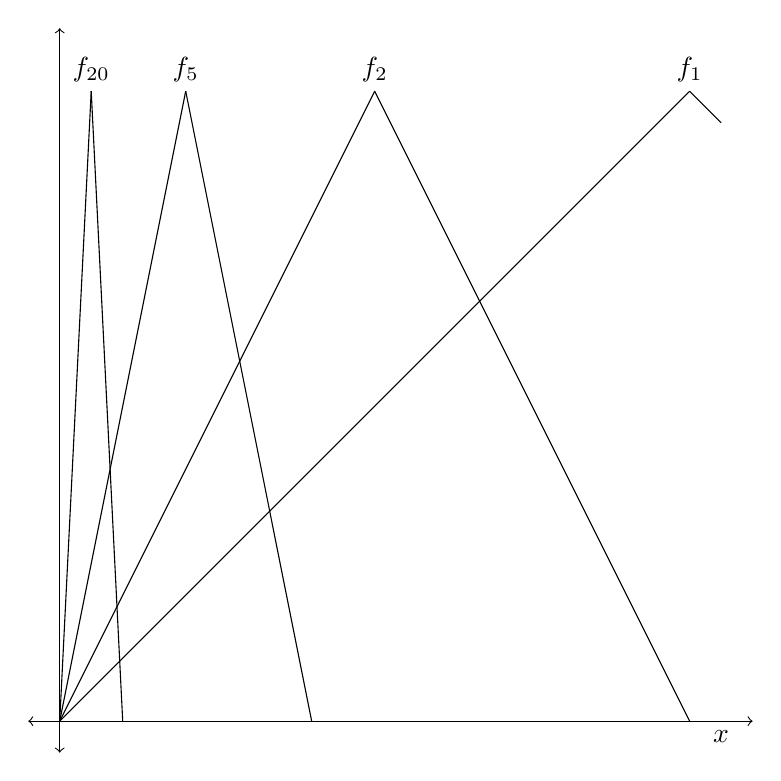
\begin{tikzpicture}[scale=8]
	
	% up
	\draw[-] (0,0) -- (1/01,1);
	\draw[-] (0,0) -- (1/02,1);
	\draw[-] (0,0) -- (1/05,1);
	\draw[-] (0,0) -- (1/20,1);

	% down
	\draw[-] (1/01,1) -- (1.05,0.95);
	\draw[-] (1/02,1) -- (2/02,0);
	\draw[-] (1/05,1) -- (2/05,0);
	\draw[-] (1/20,1) -- (2/20,0);

	% function
	\draw (1/01,1) node[anchor=south] {$f_{1}$};
	\draw (1/02,1) node[anchor=south] {$f_{2}$};
	\draw (1/05,1) node[anchor=south] {$f_{5}$};
	\draw (1/20,1) node[anchor=south] {$f_{20}$};

	% axis labels
	\draw (1.05,0) node[anchor=north] {$x$};

	% axes
	\draw[<->] (-0.05,0) -- (1.1,0);
	\draw[<->] (0,-0.05) -- (0,1.1);

\end{tikzpicture}
		\caption{Some elements of the sequence $\{ f_n \}$ from \Cref{example:uniform_convergence_1}.}
		\label{fig:mountain}
	\end{figure}
	%
	Define $f : S \to \R$ by $f(x) \coloneqq \1( x=0 )$. Obviously $f_n \conv f$ pointwise. But $\{ f_n \}$ does not converge to $f$ uniformly: $\sup_{x \in [0,2]} \abs*{f_n(x)-f(x)}=1$ no matter how large $n$ gets.
	%
\end{example}



We're defining these convergence concepts using the metric on the image space $S'$. It is perhaps more natural to define convergence of functions by endowing the functional space $F$ with a topology such that the appropriate convergence concept coincides with convergence in that topology. Convergence in the product topology (a.k.a. the topology of pointwise convergence) on $F$ is equivalent to pointwise convergence as defined above. Convergence in the topology on $F$ induced by the sup metric
%
\begin{equation*}
	d(f,g) \coloneqq \sup_{x \in S'} \rho'(f(x),g(x))
\end{equation*}
%
is equivalent to uniform convergence.


The task in this section is to extend uniform and pointwise convergence to random functions. A random function is simply a random element that takes values in a functional space. As usual, we are using the Borel $\sigma$-algebra corresponding to whatever topology we've endowed this functional space with. (There are many topologies we might want to endow a functional space with. We've already seen two, the product topology and the topology induced by the sup metric.)

Here's the (entirely straightforward) extension. We won't bother with convergence in m.s.
%
\begin{definition}
	%
	Let $(S,\rho)$ and $(S',\rho')$ be metric spaces, and let $\{ f_n \}$ and $f$ be random functions $S \to S'$.
	%
	\begin{enumerate}

		\item $f_n \convas f$ pointwise iff $\rho'(f_n(x),f(x)) \convas 0$ for every $x \in S$.

		\item $f_n \convas f$ uniformly iff $\sup_{x \in S} \rho'\left( f_n(x), f(x) \right) \convas 0$.

		\item $f_n \convp f$ pointwise iff $\rho'(f_n(x),f(x)) \convp 0$ for every $x \in S$.

		\item $f_n \convp f$ uniformly iff $\sup_{x \in S} \rho'\left( f_n(x), f(x) \right) \convp 0$.

	\end{enumerate}
	%
\end{definition}

\begin{remark}
	%
	Obvious equivalences: $f_n \convas f$ pointwise iff $f_n(x) \convas f(x)$ for every $x \in \R$, and $f_n \convp f$ pointwise iff $f_n(x) \convp f(x)$ for every $x \in \R$.
	%
\end{remark}


Some final (dull) remarks on terminology. Sometimes we're interested in convergence a.s./in probability pointwise/\allowbreak uniformly on some subset $T \subseteq S$; in this case, simply replace `for every $x \in S$ with `for every $x \in T$' and `$\sup_{x \in S}$' with `$\sup_{x \in T}$' in the definitions above. When we're holding an argument fixed, as in `$f_n(\cdot,y) \convas f(\cdot,y)$ uniformly on $T \subseteq S$', we sometimes say `$f_n(x,y) \convas f(x,y)$ uniformly in $x \in T$' instead; similarly for uniform convergence in probability.



%%%%%%%%%%%%%%%%%%%%%%%%%%%%%%%%%%%%%%%%%%%%%%%%%%%%%
\subsection{Convergence of measures}
\label{sec:modes_of_convergence:convergence_measures}
%%%%%%%%%%%%%%%%%%%%%%%%%%%%%%%%%%%%%%%%%%%%%%%%%%%%%

All three of the convergence concepts we've given have a similar flavour: they require the random elements $X_n$ to get close to $X$ as $n$ increases. But we might also care about the \emph{distributions} of $\{ X_n \}$ getting close to the distribution of $X$. For example, suppose $X_n \sim \mathcal{N}(0,1)$ and $X \sim \mathcal{N}(0,1)$, all independent.%
	\footnote{$\mathcal{N}\left(\mu,\sigma^2\right)$ denotes the normal distribution; in particular I sometimes use it to mean a normally distributed random variable, sometimes a normal law on $(\R,\mathcal{B})$. `$\sim$' reads `is distributed as'.}
No matter how large $n$ gets, $\PP( X_n \neq X )=1$. Nevertheless, it seems that this is a (trivial) case in which the distributions of $\{ X_n \}$ converge to the distribution of $X$.


For a probability space $(\Omega,\mathcal{A},\PP)$ with $\Omega$ is endowed with a topology, call $A \in \mathcal{A}$ a $\PP$-continuity set iff $\PP( \partial A) = 0$.%
	\footnote{$\partial A$ denotes the boundary of $A$. It is measurable since it's closed and we're using (a superset of) the Borel $\sigma$-algebra.}
%
\begin{definition}
	%
	Let $\{ X_n \}$ and $X$ be random elements of a metric space $(S,\rho)$ defined on $(\Omega,\mathcal{A},\PP)$. $\{ X_n \}$ converges in distribution to $X$ iff $\mathcal{L}_{X_n}(A) \conv \mathcal{L}_X(A)$ for every $\mathcal{L}_X$-continuity set $A$. Convergence in distribution is typeset $X_n \convd X$ or $X_n \rightsquigarrow X$.
	%
\end{definition}

In the case of random vectors, this obviously reduces to the (perhaps more familiar) definition that $F_{X_n} \conv F_X$ (pointwise) at every continuity point of $F_X$. The following example illustrates why we do not require convergence at discontinuity points of $F_X$.
%
\begin{example}
	%
	Let $\{X_n\}$ be a sequence of logistically distributed random variables. In particular, let them have CDFs
	%
	\begin{equation*}
		F_{X_n}(x) = \left( 1 + \exp\left( -x / \theta_n \right) \right)^{-1}
		\quad\forall x \in \R
	\end{equation*}
	%
	where the sequence $\{\theta_n\}$ satsifies $\theta_n \conv 0$. The sequence of functions $\{ F_{X_n} \}$ converges pointwise to
	%
	\begin{equation*}
		G(x) \coloneqq
		\begin{cases}
			0 & x < 0 \\
			0.5 & x = 0 \\
			1 & x > 0 .
		\end{cases} 
	\end{equation*}
	%
	$G$ is not a CDF since it isn't right-continuous. But the function $F$ given by $F(x) \coloneqq G(x)$ at $x \neq 0$ and $F(0) \coloneqq 1$ is a CDF, corresponding to a point mass at $0$. This is intuitively what the sequence $\{ X_n \}$ should converge in distribution to. And since convergence in distribution does not require convergence of the CDFs at discontinuity points, we have $X_n \convd X$ where $X$ is any random variable with this CDF.
	%
\end{example}


We say that a sequence of random variables converges in distribution, but it is really more natural to think of the sequence of laws $\{ \mathcal{L}_{X_n} \}$ as converging. In this language, convergence in distribution is called weak convergence.
%
\begin{definition}
	%
	Let $\{ \mu_n \}$ and $\mu$ be measures defined on a measurable space $(\Omega,\mathcal{A})$, and equip $\Omega$ with a topology. $\{ \mu_n \}$ converges weakly to $\mu$ iff $\mu_n(A) \conv \mu(A)$ for every $\mu$-continuity set $A$. Weak convergence is typeset $\mu_n \Rightarrow \mu$. (Occasionally, I may sloppily say that the random variables $\{X_n\}$ converge weakly to $X$.)
	%
\end{definition}


This quite intuitive notion of convergence turns out to be equivalent to several other tractable (but less intuitive) properties. The equivalence is given by the Portmanteau lemma, a small part of which is stated below. As it happens, property (2) below is conventionally taken as the definition of weak convergence.
%
\begin{lemma}[partial Portmanteau lemma]
	%
	\label{lemma:Portmanteau}
	%
	Let $\{\mu_n\}$ and $\mu$ be measures on $(\Omega,\mathcal{A})$. The following are equivalent.
	%
	\begin{enumerate}

		\item $\mu_n(A) \conv \mu(A)$ for every $\mu$-continuity set $A$.

		\item $\int_\Omega f \dd \mu_n \conv \int_\Omega f \dd \mu$ for every continuous and bounded $f : \Omega \to \R$.

	\end{enumerate}
	%
\end{lemma}


Weak convergence is equivalent to convergence in the weak$^\star$ topology on the set of probability measures on $(\Omega,\mathcal{A})$. (This is immediate from the definition of the weak$^\star$ topology!) Moreover, this topology is metrisable (by the Prohorov metric; see \textcite[][pp. 72--3]{Billingsley1999}), so weak convergence corresponds to ordinary convergence in a certain metric on the space of probability measures.

Our interest in weak convergence is motivated by central limit theorems, which concern weak convergence of the laws of normalised sums of random vectors to a normal law. It turns out that for the special case of random vectors, the theory of weak convergence can be studied using the characteristic transform introduced in \cref{sec:modes_of_convergence:characteristic_functions} below. We therefore won't delve any deeper into the theory of weak convergence in general metric spaces here. (For the curious, \textcite{Billingsley1999} is a standard book.)



%%%%%%%%%%%%%%%%%%%%%%%%%%%%%%%%%%%%%%%%%%%%%%%%%%%%%%%
\subsection{Relationships between modes of convergence}
\label{sec:modes_of_convergence:relationships}
%%%%%%%%%%%%%%%%%%%%%%%%%%%%%%%%%%%%%%%%%%%%%%%%%%%%%%%

In this section, we will establish the implication relationships between the modes of convergence we're considering. In particular, we will show that
%
\begin{equation*}
	\begin{aligned}
		\left(X_n \convas X\right)& \\
		\left(X_n \convms X\right)&
	\end{aligned}
	\Rightarrow
	\left(X_n \convp X\right)
	\Rightarrow
	\left(X_n \convd X\right) .
\end{equation*}
%
We'll also show that for a constant $\alpha$, $\bigl(X_n \convd \alpha\bigr) \Rightarrow \bigl(X_n \convp \alpha\bigr)$.


We begin with the first two implications: that a.s. convergence and convergence in m.s. imply convergence in probability. Both have nice, short proofs.

\begin{proposition}
	%
	If $X_n \convas X$, then $X_n \convp X$.
	%
\end{proposition}


\begin{proof}
	%
	Let $X_n \convas X$. Fix an $\eps>0$. Obviously $\rho(X_N,X)>\eps$ implies that $\sup_{n \geq N} \rho(X_n,X) > \eps$. Together with nonnegativity, this yields
	%
	\begin{equation*}
		0
		\leq \PP\left( \rho(X_N,X) > \eps \right)
		\leq \PP\left( \sup_{n \geq N} \rho(X_n,X) > \eps \right) .
	\end{equation*}
	%
	Since the RHS converges to $0$ as $N \conv \infty$ by $X_n \convas X$, it follows that $\lim_{N\to\infty} \PP\left( \rho(X_N,X) > \eps \right) = 0$. Since $\eps>0$ was arbitrary, $X_n \convp X$.
	%
\end{proof}


\begin{proposition}
	%
	\label{proposition:convms_implies_convp}
	%
	If $X_n \convms X$, then $X_n \convp X$.
	%
\end{proposition}

\begin{proof}
	%
	Let $X_n \convms X$. $\left(\norm{X_n-X}_2\right)^2$ is a nonnegative random variable, so Markov's inequality (p. \pageref{proposition:Markovs_inequality}) applies. Together with the fact that probabilities are nonnegative, we have for any $\eps>0$ that
	%
	\begin{multline*}
		0
		\leq \PP\left( \norm{X_n-X}_2 > \eps \right) 
		= \PP\left( \left(\norm{X_n-X}_2\right)^2 > \eps^2 \right)
		\\
		\leq \eps^{-2} \E\left( \left(\norm{X_n-X}_2\right)^2 \right) .
	\end{multline*}
	%
	The RHS converges to $0$ since $X_n \convms X$. Hence $\PP( \norm{X_n-X}_2 > \eps ) \conv 0$ for every $\eps>0$, i.e. $X_n \convp X$.
	%
\end{proof}

A natural question you might now ask is: convergence in probability plus what property is equivalent to convergence in mean square? The answer is a boundedness property called uniform integrability; see e.g. \textcite[][sec. 13.7]{Williams1991}.


To show that a.s. convergence and convergence in m.s. do not imply each other, we give counterexamples.

\begin{example}[$\convms$ without $\convas$]
	%
	Let $\{ X_n \}$ be independent with
	%
	\begin{equation*}
		\PP(X_n=0) = 1-\tfrac{1}{n} 
		\quad\text{and}\quad
		\PP(X_n=1) = \tfrac{1}{n}
		\quad\text{for each $n \in \N$.}
	\end{equation*}
	%
	Then $\E\left( X_n^2 \right) = 1/n \conv 0$ as $n\conv\infty$, so $X_n \convms 0$.

	It's obvious (but we didn't prove) that if $\{ X_n \}$ is a.s.-convergent then the limit must be $0$. A.s. convergence to $0$ would require that
	%
	\begin{equation*}
		\lim_{N\to\infty} \PP\left( \sup_{n \geq N} \abs{X_n} < \eps \right) = 1 
		\quad\text{for every $\eps>0$.}
	\end{equation*}
	%
	So choose $\eps \in (0,1)$. Then $\abs{X_n}<\eps$ iff $X_n=0$, so for any $N \in \N$ we have
	%
	\begin{equation*}
		\PP\left( \sup_{n \geq N} \abs{X_n} < \eps \right)
		= \PP( X_n=0 \;\;\forall n \geq N )
		= \prod_{n=N}^\infty \left( 1 - \tfrac{1}{n} \right) .
	\end{equation*}
	%
	where the final equality used independence. Taking logs and using the inequality $\ln\left(1-\tfrac{1}{n}\right) \leq -\tfrac{1}{n}$,%
		\footnote{Since $\ln$ is concave, it must lie below all its tangents, i.e. for any $x,x' >0$, $\ln(x) \leq \ln(x') + (x')^{-1} (x-x')$. Setting $x=1-\tfrac{1}{n}$ and $x'=1$ yields $\ln\left(1-\tfrac{1}{n}\right) \leq -\tfrac{1}{n}$.}
	%
	\begin{equation*}
		\ln \left( \PP\left( \sup_{n \geq N} \abs{X_n} < \eps \right) \right)
		= \sum_{n=N}^\infty \ln \left( 1 - \tfrac{1}{n} \right) 
		\leq - \sum_{n=N}^\infty n^{-1}
		= - \infty 
	\end{equation*}
	%
	since the harmonic series $\sum_{n=N}^\infty n^{-1}$ diverges for every $N$. So by continuity of $\ln(\cdot)$, $\PP\left( \sup_{n \geq N} \abs{X_n} < \eps \right)=0$ for every $N$, hence
	%
	\begin{equation*}
		\lim_{N\to\infty} \PP\left( \sup_{n \geq N} \abs{X_n} < \eps \right) 
		= 0 \neq 1 .
	\end{equation*}
	%
\end{example}

\begin{example}[$\convas$ without $\convms$]
	%
	Let $\{ X_n \}$ be independent with
	%
	\begin{equation*}
		\PP(X_n=0) = 1-\tfrac{1}{n^2} 
		\quad\text{and}\quad
		\PP(X_n=n) = \tfrac{1}{n^2}
		\quad\text{for each $n \in \N$.}
	\end{equation*}
	%
	$\E\left( X_n^2 \right) = n^2 / n^2 = 1$ for every $n \in \N$, so we don't have convergence to $0$ in mean square. It's fairly obvious (but we didn't prove) that we cannot have convergence in m.s. to anything other than $0$.

 	Again, a.s. convergence to $0$ requires that
	%
	\begin{equation*}
		\lim_{N\to\infty} \PP\left( \sup_{n \geq N} \abs{X_n} < \eps \right) = 1 
		\quad\text{for every $\eps>0$.}
	\end{equation*}
	%
	Following the steps in the previous example, for small $\eps>0$ and any $N \in \N$ we have
	%
	\begin{equation*}
		\ln\left( \PP\left( \sup_{n \geq N} \abs{X_n} < \eps \right) \right)
		= \sum_{n=N}^\infty \ln \left( 1 - \tfrac{1}{n^2} \right) .
	\end{equation*}
	%
	Using the inequality $\ln \left( 1 - \tfrac{1}{n^2} \right) \geq -\tfrac{1}{n^2} - \tfrac{1}{2n^4}$,%
		\footnote{This inequality follows from the fact that in the Taylor series
		%
		\begin{equation*}
			\ln(1+x) 
			= \sum_{n=1}^\infty \frac{(-1)^{n+1}}{n} x^n 
			= x - \frac{x^2}{2} + \sum_{n=3}^\infty \frac{(-1)^{n+1}}{n} x^n ,
		\end{equation*}
		%
		the remainder $\sum_{n=3}^\infty \frac{(-1)^{n+1}}{n} x^n$ can be shown to be nonnegative. Now set $x=-1/n^2$.}
	we obtain
	%
	\begin{equation*}
		\ln\left( \PP\left( \sup_{n \geq N} \abs{X_n} < \eps \right) \right)
		\geq - \sum_{n=N}^\infty \left( \frac{1}{n^2} + \frac{1}{2n^4} \right) .
	\end{equation*}
	%
	The $p$-series $\sum_{n=N}^\infty n^{-p}$ is convergent iff $p>1$ (regardless of $N$), so the RHS is finite for each $N$ and converges to $0$ as $N\to\infty$. So by continuity of $\ln(\cdot)$ we obtain
	%
	\begin{equation*}
		\lim_{N\to\infty} \PP\left( \sup_{n \geq N} \abs{X_n} < \eps \right) = 1 .
	\end{equation*}
	%
\end{example}

%Joel thinks (sounds right!) that when moments exist, a.s. convergence does imply convergence in m.s.


Now for another proposition: convergence in probability implies convergence in distribution.

\begin{proposition}
	%
	\label{proposition:convp_convd}
	%
	If $X_n \convp X$, then $X_n \convd X$.
	%
\end{proposition}


The statement is true for general random elements, but our proof restricts attention to random vectors in order to make use of the simpler CDF-based definition of convergence in distribution.


\begin{proof}[Proof for random vectors]
	%
	Let $X_n \convp X$. Define $Z_n \coloneqq X - X_n$, so that $Z_n \convp 0$. Fix some $\eps>0$ and a continuity point $t \in \R$ of $F_X$. We must show that $F_{X_n}(t) \conv F_X(t)$.

	Using the fact that $A \subseteq B$ implies $\PP(A) \leq \PP(B)$ and a few other basic facts about probabilities,
	%
	\begin{align*}
		F_{X_n}(t)
		={}& \PP\left( X - ( X - X_n) \leq t \right) \\
		={}& \PP\left( X \leq t + Z_n \right) \\
		={}& \PP\left( X \leq t + Z_n, Z_n < \eps \right)
		+ \PP\left( X \leq t + Z_n, Z_n \geq \eps \right) \\
		\leq{}& \PP\left( X \leq t + \eps, Z_n < \eps \right)
		+ \PP\left( X \leq t + Z_n, Z_n \geq \eps \right) \\
		\leq{}& \PP\left( X \leq t + \eps \right)
		+ \PP\left( X \leq t + Z_n, Z_n \geq \eps \right) \\
		\leq{}& \PP\left( X \leq t + \eps \right)
		+ \PP\left( X \leq \infty, Z_n \geq \eps \right) \\
		\leq{}& \PP\left( X \leq t + \eps \right)
		+ \PP\left( Z_n \geq \eps \right) \\
		={}& F_{X}\left( t + \eps \right)
		+ \PP\left( Z_n \geq \eps \right) .
	\end{align*}
	%
	Since $Z_n \convp 0$, $\PP\left( Z_n \geq \eps \right) \conv 0$ as $n \conv \infty$. It follows that
	%
	\begin{equation*}
		\limsup_{n\to\infty} F_{X_n}(t) \leq F_X(t+\eps) .
	\end{equation*}
	%
	Taking $\eps\conv 0$ and using the fact that $t$ is a continuity point of $F_X$,
	%
	\begin{equation*}
		\limsup_{n\to\infty} F_{X_n}(t) \leq F_X(t) .
	\end{equation*}
	
	Now go through the exactly same steps, replacing $F_{X_n}$ with $1-F_{X_n}$ and $\eps$ with $-\eps$:
	%
	\begin{align*}
		1 - F_{X_n}(t)
		={}& \PP\left( X - ( X - X_n) > t \right) \\
		={}& \PP\left( X > t + Z_n \right) \\
		={}& \PP\left( X > t + Z_n, Z_n \leq -\eps \right)
		+ \PP\left( X > t + Z_n, Z_n > -\eps \right) \\
		\leq{}& \PP\left( X > t + Z_n, Z_n \leq -\eps \right)
		+ \PP\left( X > t -\eps, Z_n > -\eps \right) \\
		\leq{}& \PP\left( X > t + Z_n, Z_n \leq -\eps \right)
		+ \PP\left( X > t -\eps \right) \\
		\leq{}& \PP\left( X > -\infty, Z_n \leq -\eps \right)
		+ \PP\left( X > t -\eps \right) \\
		\leq{}& \PP\left( Z_n \leq -\eps \right)
		+ \PP\left( X > t -\eps \right) \\
		={}& \PP\left( Z_n \leq -\eps \right)
		+ \left[ 1 - F_X\left( t -\eps \right) \right] .
	\end{align*}
	%
	Rearranging, $F_{X_n}(t) \geq F_X(t-\eps) - \PP\left( Z_n \leq -\eps \right)$, which yields
	%
	\begin{equation*}
		\liminf_{n\to\infty} F_{X_n}(t) \geq F_X(t-\eps) 
	\end{equation*}
	%
	since $Z_n \convp 0$. Taking $\eps\conv 0$ and using the fact that $t$ is a continuity point of $F_X$ then gives us
	%
	\begin{equation*}
		\liminf_{n\to\infty} F_{X_n}(t) \geq F_X(t) .
	\end{equation*}

	Putting together the pieces,
	%
	\begin{equation*}
		\limsup_{n\to\infty} F_{X_n}(t) 
		\leq F_X(t)
		\leq \liminf_{n\to\infty} F_{X_n}(t) .
	\end{equation*}
	%
	Hence $\{ F_{X_n}(t) \}$ is convergent and has limit $F_X(t)$.
	%
\end{proof}


There is a special case in which the converse is true:
%
\begin{proposition}
	%
	\label{proposition:convd_convp}
	%
	If $X_n \convd X$ for $X$ constant, then $X_n \convp X$.
	%
\end{proposition}

The result is pretty obvious, but the proof I've seen use parts of the Portmanteau lemma that I haven't stated, so I won't bother.



%%%%%%%%%%%%%%%%%%%%%%%%%%%%%%%%%%%%%%%%%%%%%%%
\subsection{The Borel--Cantelli lemmata}
\label{sec:modes_of_convergence:Borel--Cantelli}
%%%%%%%%%%%%%%%%%%%%%%%%%%%%%%%%%%%%%%%%%%%%%%%

The concentration inequalities in \cref{sec:probability:inequalities} (p. \pageref{sec:probability:inequalities}) can be used to prove that a sequence of random elements converges in probability. For example, if $\{ X_n \}$ are random variables with means $\mu$ and variances $n^{-\alpha} \sigma^2$ for some $\alpha>0$, then Chebychev's inequality (p. \pageref{corollary:Chebychevs_inequality}) yields
%
\begin{equation*}
	\PP( \abs*{X_n-\mu} > \eps ) \leq \frac{ \sigma^2 }{ n^\alpha \eps^2 } \conv 0
	\quad\text{for any $\eps>0$} ,
\end{equation*}
%
so $X_n \convp \mu$. (This is how we will prove Chebychev's WLLN in \cref{sec:LLNs:independence_variance_restrictions} (p. \pageref{sec:LLNs:independence_variance_restrictions}).)

It would be nice to have a similarly tractable sufficient condition for almost sure convergence. That is exactly what the first Borel--Cantelli lemma gives us. And there's more: the second Borel--Cantelli lemma says that our sufficient condition is also necessary when the sequence is independent.
%
\begin{theorem}[Borel--Cantelli lemmata]
	%
	Let $\{ X_n \}$ and $X$ be random elements of a metric space $(S,\rho)$ defined on $(\Omega,\mathcal{A},\PP)$.
	%
	\begin{enumerate}

		\item If $\sum_{n=1}^\infty \PP( \rho(X_n,X) > \eps ) < \infty$ for all $\eps>0$, then $X_n \convas X$.

		\item If $\sum_{n=1}^\infty \PP( \rho(X_n,X) > \eps ) = \infty$ for some $\eps>0$ and $\{ X_n \}$ are independent, then $X_n$ does not converge a.s. to $X$.

	\end{enumerate}
	%
\end{theorem}

The Borel--Cantelli lemmata are actually much more general than what we stated here. If you care, see e.g. \textcite[][Theorem 3.4.2]{Rosenthal2006}.



%%%%%%%%%%%%%%%%%%%%%%%%%%%%%%%%%%%%%%%%%%%%%%%%
\subsection{Convergence of moments}
\label{sec:modes_of_convergence:conv_of_moments}
%%%%%%%%%%%%%%%%%%%%%%%%%%%%%%%%%%%%%%%%%%%%%%%%

Suppose $X_n \convd X$ for random variables $\{ X_n \}$ and $X$. It might seem reasonable to conjecture that $\E(X_n) \conv \E(X)$. But upon reflection, it's not a very good conjecture: by the Portmanteau lemma (p. \pageref{lemma:Portmanteau}), $X_n \convd X$ is equivalent to
%
\begin{equation*}
	\int_\R f \dd \mathcal{L}_{X_n} \conv \int_\R f \dd \mathcal{L}_X
	\quad\text{for every continuous and bounded $f$} ,
\end{equation*}
%
but we want
%
\begin{equation*}
	\int_\R I \dd \mathcal{L}_{X_n} \conv \int_\R I \dd \mathcal{L}_X
\end{equation*}
%
where $I$ is the definitely-not-bounded identity function $I(x) \coloneqq x$! So $\{ \mathcal{L}_{X_n} \}$ are going to have to be appropriately bounded if the moments are to converge.


I'll give two counterexamples. In the first, no moments exist along the sequence, but the limit distribution has moments. In the (perhaps less trivial) second example, moments exist along the entire sequence, but fail to converge nonetheless.
%
\begin{example}
	%
	Let $\{ X_n \}$ be independent random variables with CDFs
	%
	\begin{equation*}
		F_{X_n}(x) \coloneqq \tfrac{1}{n} C(x) + \left(1-\tfrac{1}{n}\right) \Phi(x)
	\end{equation*}
	%
	where $\Phi$ is the standard normal CDF and $C$ is the standard Cauchy CDF
	%
	\begin{equation*}
		C(x) \coloneqq \tfrac{1}{2} + \pi^{-1} \arctan(x) .
	\end{equation*}
	%
	It's obvious that $F_{X_n} \conv \Phi$ pointwise, so $X_n \convd \mathcal{N}(0,1)$. The expectation of the limit is therefore $0$. But $X_n$ has no mean for any $n \in \N$ since the Cauchy distribution has no moments. So the sequence $\{ \E(X_n) \}$ does not even exist, hence certainly cannot be said to converge to zero.
	%
\end{example}
%
\begin{example}
	%
	Consider random variables $\{ X_n \}$ and $X$ such that
	%
	\begin{equation*}
		\PP(X_n=1) = 1 - \tfrac{1}{n}
		\quad\text{and}\quad
		\PP(X_n=n)=\tfrac{1}{n} 
	\end{equation*}
	%
	and $X \sim \mathcal{N}(0,1)$, with $X$ independent of $\{ X_n \}$. Define $Y_n \coloneqq (X_n X)^2$. Evidently $X_n^2 \convp 1$, so by Slutsky's theorem $Y_n = X_n^2 X^2 \convd X^2$. But $\E\left( X^2 \right)=1$, whereas (using independence)
	%
	\begin{equation*}
		\E\left( Y_n \right)
		= \E\left( X_n^2 \right) \E\left( X^2 \right)
		= \E\left( X_n^2 \right)
		= \left( 1 - \tfrac{1}{n} \right) + \tfrac{1}{n} n^2
		\conv \infty .
	\end{equation*}
	%
\end{example}

But even if $X_n \convd X$ is not sufficient for $\E(X_n) \conv \E(X)$, surely $X_n \convas X$ is sufficient? No again! We can still get the sort of pathological behaviour exhibited by the examples above. To rule this out, we need a boundedness condition on $\{ X_n \}$ and $X$ to rule out nonexistence or explosive behaviour.

There are several important theorems giving conditions under which $X_n \convas X$ implies $\E(X_n) \conv \E(X)$. These include (in order from strongest to weakest assumptions) the monotone convergence theorem, the bounded convergence theorem, the (Lebesgue) dominated convergence theorem and the (Vitali) uniform integrability convergence theorem. The proofs of the last few rely heavily on Fatou's lemma. All of this is covered well by \textcite[][mainly ch. 9]{Rosenthal2006}. We'll need the dominated convergence theorem later on, but I won't give a proof.
%
\begin{theorem}[dominated convergence theorem]
	%
	\label{theorem:dominated_convergence}
	%
	Let $\{ X_n \}$, $X$ and $Y$ be random variables such that $X_n \convas X$, $\abs*{X_n} \leq Y$ (pointwise) for each $n \in \N$, and $\E(Y)$ exists and is finite. Then $\E(X_n) \conv \E(X)$.
	%
\end{theorem}

In other words, when $X_n \convas X$, a sufficient condition for $\int_\Omega X_n \dd\PP \conv \int_\Omega X \dd\PP$ is that $\{ X_n \}$ is dominated by an integrable function (random variable) $Y$.



%%%%%%%%%%%%%%%%%%%%%%%%%%%%%%%%%%%%%%%%%%%%%%%%%%%%%%%%%
\subsection{Characteristic functions}
\label{sec:modes_of_convergence:characteristic_functions}
%%%%%%%%%%%%%%%%%%%%%%%%%%%%%%%%%%%%%%%%%%%%%%%%%%%%%%%%%

When we're working with random vectors, we have access to the following highly convenient object. Let $\C$ denote the complex plane.

\begin{definition}
	%
	Let $X$ be a random $n$-vector on $(\Omega,\mathcal{A},\PP)$. The characteristic function of $X$ is $\phi_X : \R^n \to \C$ given by
	%
	\begin{equation*}
		\phi_X(t) 
		\coloneqq \E \left( \exp\left( i t^\trans X \right) \right)
		= \int_{\R^n} \exp\left( i t^\trans x \right) \mathcal{L}_X(\dd x)
		\quad\text{for each $t \in \R^n$} .%
			\footnote{Since $\abs*{\exp(ic)} = 1$ for any $c \in \R$, $\exp\left( i t^\trans X \right)$ is $\PP$-integrable for any $t$. Hence $\phi_X$ is always well-defined, unlike the otherwise similar moment-generating function.}
	\end{equation*}
	%
\end{definition}


Above, we took the random variable $X$ as the primitive. Although this is often natural, most of probability theory is concerned with measures, not random variables. It is therefore instructive to study the mapping $\mu \mapsto \phi^\mu$ from probability measures to the characteristic functions of random variables distributed according to those probability measures:

\begin{definition}
	%
	The characteristic transform is the mapping $\mu \mapsto \phi^\mu$ from probability measures $\mu$ on $\left(\R^n,\mathcal{B}\right)$ to characteristic functions $\phi^\mu : \R^n \to \C$, defined by
	%
	\begin{equation*}
		\phi^\mu(t) 
		\coloneqq \int_{\R^n} \exp\left( i t^\trans x \right) \mu(\dd x)
		\quad\text{for each $t \in \R^n$} .%
			\footnote{The characteristic transform is also sometimes known as (a version of) the Fourier transform. But what exactly is meant by `Fourier transform' varies hugely between authors and fields, so I won't use this term at all.}
	\end{equation*}
	%
\end{definition}

This definition might make you wonder what the space of characteristic functions is. It is by no means the case that every function $\R^n \to \C$ is the characteristic transform of some probability measure on $\left(\R^n,\mathcal{B}\right)$! It is possible to state `primitive' necessary and sufficient conditions for a function $\R^n \to \C$ to be a characteristic function. Bochner's theorem (e.g. \textcite[][p. 141]{Rao1973}) gives one set of necessary and sufficient conditions. Tractable sufficient (but not necessary) conditions are given by Pólya's theorem, which I'll only state for the univariate case.
%
\begin{theorem}[Pólya's theorem]
	%
	Suppose $\varphi : \R \to \C$ is $\R$-valued, even,%
		\footnote{A function $f$ is even iff $f(-x)=f(x)$ for every $x$ in its domain.}
	continuous, convex on $\R_{++}$, and satisfies $\varphi(0)=1$ and $\lim_{t\to\infty} \varphi(t)=0$. Then $\varphi = \phi^\mu$ for some probability measure $\mu$ on $(\R,\mathcal{B})$ that is absolutely continuous w.r.t. Lebesgue measure and symmetric about 0.
	%
\end{theorem}


It turns out that the space of characteristic functions is a dual of the space of probability measures in the following sense. First, the characteristic mapping is a bijection: $\phi^\mu=\phi^\nu$ (pointwise) iff $\mu=\nu$ (setwise). Second, the characteristic transform has a closed-form inverse, and there are many convenient equivalences between properties of probability measures and properties of characteristic functions. Third, the characteristic mapping is continuous in a certain sense.

Let's state two important bits of that formally. Proofs can be found in e.g. \textcite[][ch. 10]{Rosenthal2006}.
%
\begin{theorem}[Fourier uniqueness theorem]
	%
	Let $\mu$ and $\nu$ be probability measures on $\left(\R^n,\mathcal{B}\right)$. Then $\phi^\mu=\phi^\nu$ (pointwise) iff $\mu=\nu$ (setwise).	
	%
\end{theorem}
%
\begin{theorem}[Lévy's continuity theorem]
	%
	\label{theorem:Levys_continuity_theorem}
	%
	Let $\{ \mu_n \}$ and $\mu$ be probability measures on $\left(\R^n,\mathcal{B}\right)$. Then $\mu_n \Rightarrow \mu$ iff $\phi^{\mu_n} \conv \phi^\mu$ pointwise.%
		\footnote{It's called the continuity theorem because when the space of probability measures is endowed with the topology of weak convergence (the weak$^\star$ topology) and the space of characteristic functions is endowed with the topology of pointwise convergence (the product topology), the theorem says precisely that the characteristic transform and its inverse are continuous mappings.}	
	%
\end{theorem}


These properties mean that any results we prove about characteristic functions, including convergence results, translate directly into results about probability measures (and vice versa). When we face a difficult question about probability measures on $\left(\R^n,\mathcal{B}\right)$, we will often translate it into a question about characteristic functions, easily find the answer, then translate the answer back into probability-measure space.

The leading example of this strategy is the proof of the Lindeberg--Lévy central limit theorem (p. \pageref{theorem:Lindeberg-Levy}). But we'll also use it to prove part of the continuous mapping theorem on p. \pageref{proof:CMT_3}, and to establish an interesting property of the Cauchy distribution in an example on p. \pageref{example:Cauchy_LLN}.


I mentioned equivalences between properties of measures and of their characteristic transforms. There are many, and they are easy to look up, but here are a few important ones.
%
\begin{proposition}
	%
	\label{proposition:characteristic_fn_properties}
	%
	Let $X$ and $Y$ be random variables.
	%
	\begin{enumerate}

		\item $\phi_X(0)=1$.

		\item $\abs*{\phi_X(t)}=1$ for every $t \in \R^n$.

		\item $\phi_{aX+b}(t) = \exp(itb) \phi_X(at)$ for any $a \in \R$ and $b,t \in \R$.

		\item $\phi_{X+Y} = \phi_X \phi_Y$ if $X$ and $Y$ are independent. (The converse is not true!)

		\item If $\E\left(X^j\right)$ exists and is finite then $\phi_X^{(j)}(0)$ exists. (There's a partial converse.) Whenever they exist and are finite, $\phi_X^{(j)}(0) = i^j \E\left(X^j\right)$.

		\item $\phi_X$ is uniformly continuous.

		\item (Riemann--Lebesgue lemma) If $\mathcal{L}_X$ has a density w.r.t. Lebesgue measure, then $\phi_X(t) \conv 0$ as $\abs{t} \conv \infty$.

	\end{enumerate}
	%
\end{proposition}
%


Finally, an illustration.
%
\begin{example}[the Cauchy law is stable]
	%
	\label{example:Cauchy_LLN}
	%
	A Cauchy-distributed random variable $X$ is one whose density w.r.t. Lebesgue measure is
	%
	\begin{equation*}
		\frac{\dd \mathcal{L}_X}{\dd \lambda}
		= \frac{1}{\sqrt{\pi}} \frac{1}{1+x^2} .
	\end{equation*}
	%
	A patient reader can verify that the corresponding characteristic function is $\phi_X(t) = \exp(-\abs{t})$. We know that the Cauchy distribution has no moments, so it shouldn't surprise us that $\phi_X$ is not differentiable at $0$.%
		\footnote{Above, we stated the result that when a moment exists and is finite, the corresponding derivative exists. We did not state the partial converse. So this does not constitute a proof that the Cauchy distribution has no moments!}

	Now consider a sequence $\{ X_n \}$ of independent Cauchy-distributed random variables, and write $S_n \coloneqq n^{-1} \sum_{i=1}^n X_i$. Then
	%
	\begin{align*}
		\phi_{S_n}(t)
		={}& \E\left( \exp\left( it n^{-1} \sum_{i=1}^n X_i \right) \right)
		\\
		={}& \E\left( \prod_{i=1}^n \exp\left( it n^{-1} X_i \right) \right)
		\\
		={}& \prod_{i=1}^n \E\left( \exp\left( it n^{-1} X_i \right) \right)
		\\
		={}& \E\left( \exp\left( it n^{-1} X_1 \right) \right)^n
		\\
		={}& \phi_{X_1}\left( t / n \right)^n
		\\
		={}& \exp\left( -\abs{t}/n \right)^n
		\\
		={}& \exp\left( -\abs{t} \right) 
		\\
		={}& \phi_{X_1}\left( t \right) .
	\end{align*}
	%
	So the average of $n$ Cauchy-distributed random variables is itself Cauchy-distributed!
	$n$-fold convolution of the Cauchy distribution is itself Cauchy! A distribution with the property that $aS_n$ for some $a$ has the same distribution as $X_1$ is called a (Lévy or $\alpha$) stable distribution. Another stable law is the normal distribution (you already knew that---think about it). The theory of stable laws is a very interesting branch of probability theory, I think.%
		\footnote{\label{footnote:stable_laws}Think of a sequence of distributions of $S_n$ as a path in the space of probability distributions. This path is governed by a law of motion. A stable distribution is a steady state of this law of motion: once you're there, you don't leave. Some of these steady states may be attractors in some region: if you start in this region, the sequence converges weakly to the stable law. One theorem in the theory of stable laws is (loosely) that only stable laws can be attractors.

		Moreover, there are generalisations of the central limit theorems. CLTs give (large) regions in which the normal law is an attractor; `generalised central limit theorems' give large regions in which the CLT fails (due to infinite variance), but in which there is another attractor. By the previous result, this attractor must be a stable distribution, but it will not be normal. This material can be found in e.g. \textcite[][ch. 7]{GnedenkoKolmogorov1954} and \textcite[][sec. 3.7]{Durrett2010}.}

	This example also serves as a prelude to our study of laws of large numbers, which give conditions under which $S_n$ converges (a.s. or in probability) to a constant. It should be obvious that $S_n$ converges weakly to a Cauchy law; we don't even need Lévy's continuity theorem to prove this. Convergence to a point fails to happen here because the Cauchy distribution has `heavy tails', i.e. lots of probability mass in the tails. (The formal definition of `heavy tail' is usually that the variance is infinite.) As we will see when we prove LLNs, moment restrictions are required in order to avoid this sort of problem. (At the very least, we'll require the first moment to exist.)
	%
\end{example}



%%%%%%%%%%%%%%%%%%%%%%%%%%%%%%%%%%%%%%%%%%%
\subsection{The continuous mapping theorem}
\label{sec:modes_of_convergence:CMT}
%%%%%%%%%%%%%%%%%%%%%%%%%%%%%%%%%%%%%%%%%%%

One characterisation of continuity in metric spaces is that a continuous mapping is one that `preserves convergence': $f$ is continuous at $x_0$ iff $f(x_n) \conv f(x_0)$ for any sequence $\{ x_n \}$ s.t. $x_n \conv x_0$. The Mann--Wald continuous mapping theorem (CMT) is the analog for random variables of the `only if' part of this characterisation: it says that a.s. convergence, convergence in probability and convergence in distribution are all preserved under almost-everywhere continuous transformations.
%
\begin{theorem}[Mann--Wald CMT]
	%
	\label{theorem:Mann--Wald_CMT}
	%
	Let $(S,\rho)$ and $(S',\rho')$ be metric spaces, let $\{ X_n \}$ and $X$ be random elements of $(S,\rho)$, and let $g : S \to S'$ be measurable and continuous $\mathcal{L}_X$-a.e.%
		\footnote{Recall that $\mathcal{L}_X$ is the law of $X$. So the final requirement is that the underlying probability space $(\Omega,\mathcal{A},\PP)$ satisfies $\PP\left(\left\{ \omega \in \Omega : \text{$g$ continuous at $X(\omega)$} \right\}\right)=1$.}
	Then
	%
	\begin{enumerate}

		\item $X_n \convas X$ implies $g(X_n) \convas g(X)$.

		\item $X_n \convp X$ implies $g(X_n) \convp g(X)$.

		\item $X_n \convd X$ implies $g(X_n) \convd g(X)$.

	\end{enumerate}
	%
\end{theorem}


\begin{remark}
	%
	We did not mention convergence in mean square because it turns out not to be preserved under arbitrary a.e.-continuous mappings! Something much stronger is needed, e.g. $g$ linear.
	%
\end{remark}


\begin{proof}[Proof of (1)]
	%
	We know that there are measurable $\Omega',\Omega'' \subseteq \Omega$ such that $X_n(\omega) \conv X(\omega)$ for all $\omega \in \Omega'$, $g$ is continuous at all $X(\omega)$ s.t. $\omega \in \Omega''$, and $\PP(\Omega')=\PP(\Omega'')=1$. Firstly, $\Omega' \intersect \Omega''$ is measurable with $\PP\left( \Omega' \intersect \Omega'' \right) = 1$ since
	%
	\begin{equation*}
		\PP\left( \Omega' \intersect \Omega'' \right)
		= 1 - \PP\left( \left( \Omega' \right)^\compl 
		\union \left( \Omega'' \right)^\compl \right)
		\geq 1 - \PP\left( \left( \Omega' \right)^\compl \right)
		- \PP\left( \left( \Omega'' \right)^\compl \right)
		= 1 .
	\end{equation*}
	%
	Secondly, $g(X_n(\omega)) \conv g(X(\omega))$ at all $\omega \in \Omega' \intersect \Omega''$.
	%
\end{proof}


We won't bother proving (2) in full generality, though it is not hard. Instead, we will content ourselves with the case in which $X_n \convp \alpha$ for a constant $\alpha$. In this case, continuity $\mathcal{L}_X$-a.e. of $g$ reduces to continuity of $g$ at $\alpha$.

\begin{proof}[Proof of (2) for constant $X$]
	%
	By continuity of $g$ at $\alpha$, for each $\eps>0$, there is a $\delta>0$ such that $\rho(X_n,\alpha)<\delta$ implies $\rho'(g(X_n),g(\alpha))<\eps$. So
	%
	\begin{equation*}
		1
		\geq \PP\left( \rho'(g(X_n),g(\alpha)) < \eps \right) 
		\geq \PP( \rho(X_n,\alpha) < \delta ) .
	\end{equation*}
	%
	Since $X_n \convp \alpha$, the right-hand side converges to $1$ regardless of $\delta$. It follows that $\PP\left( \rho'(g(X_n),g(\alpha)) < \eps \right) \conv 1$ for each $\eps>0$, i.e. $g(X_n) \convp g(\alpha)$.
	%
\end{proof}


For (3), the cleanest general proof that I've seen uses Skorokhod's theorem, then follows the argument for (1). This would take us too far afield, so let's restrict attention to the case in which $\{ X_n\}$ and $X$ are random $\ell$-vectors and $g : \R^\ell \to \R^m$, so that we can use characteristic functions.

\begin{proof}[Proof of (3) for $S=\R^\ell$ and $S'=\R^m$]
	%
	\label{proof:CMT_3}
	%
	Fix $t \in \R^\ell$; we wish to show that $\phi_{g(X_n)}(t) \conv \phi_{g(X)}(t)$. We have
	%
	\begin{align*}
		\phi_{g(X_n)}(t)
		={}& \int_{\R^\ell} \exp\left( i t^\trans g(y) \right) \mathcal{L}_{X_n}( \dd y )
		\\
		={}& \int_{\R^\ell} \cos\left( t^\trans g(y) \right) \mathcal{L}_{X_n}( \dd y ) 
		+ i \int_{\R^\ell} \sin\left( t^\trans g(y) \right) \mathcal{L}_{X_n}( \dd y ) .
		\\
		\conv& \int_{\R^\ell} \cos\left( t^\trans g(y) \right) \mathcal{L}_X( \dd y ) 
		+ i \int_{\R^\ell} \sin\left( t^\trans g(y) \right) \mathcal{L}_X( \dd y ) 
		\\
		={}& \int_{\R^\ell} \exp\left( i t^\trans g(y) \right) \mathcal{L}_X( \dd y )
		\\
		={}& \phi_{g(X)}(t) 
	\end{align*}
	%
	where convergence follows by the Portmanteau lemma (p. \pageref{lemma:Portmanteau}),%
		\footnote{Joel actually appealed to the Helly--Bray theorem, which is a special case of the Portmanteau lemma.}
	since $y \mapsto \cos\left( t^\trans g(y) \right)$ and $y \mapsto \sin\left( t^\trans g(y) \right)$ are bounded and continuous mappings. Hence $g(X_n) \convd g(X)$ by Lévy's continuity theorem (p. \pageref{theorem:Levys_continuity_theorem}).
	%
\end{proof}



The following result is an oft-used corollary to the continuous mapping theorem. It states that the elementary algebraic operations of addition, multiplication and division are preserved under weak convergence. (It's a corollary because these operations are continuous.)
%
\begin{corollary}[Slutsky's theorem]
	%
	\label{corollary:Slutsky}
	%
	Let $\{ X_n \}$ and $X$ be $m\times k$ random matrices, let $\{ Y_n \}$ be $k \times k$ random matrices, and let $A$ be a $k \times k$ (constant) matrix. Suppose that $X_n \convd X$ and $Y_n \convp A$. Then
	%
	\begin{enumerate}

		\item $X_n + Y_n \convd X + A$.

		\item $X_n Y_n \convd X A$.

		\item $X_n Y_n^{-1} \convd X A^{-1}$ provided $A$ is invertible.%
			\footnote{If some $\{ Y_n \}$ in (3) are singular, we can replace $Y_n^{-1}$ with a Moore--Penrose pseudo-inverse and still obtain convergence. The Moore--Penrose pseudo-inverse is continuous at invertibility points, so the continuous mapping theorem applies. (But note that unlike the ordinary matrix inverse, the Moore--Penrose pseudo-inverse is not continuous at all points.)}

	\end{enumerate}
	%
\end{corollary}


\begin{proof}
	%
	$(X,A)$ and each $(X_n,Y_n)$ are random elements of the metric space $\R^{m \times k} \times \R^{k \times k}$. $Y_n \convp A$ implies $Y_n \convd A$ by \Cref{proposition:convd_convp} (p. \pageref{proposition:convd_convp}). The mappings $(x,y) \mapsto x+y$ and $(x,y) \mapsto xy$ are continuous, and $(x,y) \mapsto xy^{-1}$ is continuous whenever $y$ is invertible. The result then follows from part (3) of the continuous mapping theorem.
	%
\end{proof}

%For a direct proof of Slutsky's theorem, see \textcite[][pp. 122--3]{Rao1973}. One way to prove part (1) directly is to imitate the proof of \Cref{proposition:convp_convd} (p. \pageref{proposition:convp_convd}), setting $Z_n \coloneqq (X_n+Y_n) - (X+\alpha)$ and then arduously bounding the $\limsup$ and $\liminf$ to establish convergence in distribution.




\begin{remark}
	%
	Since the proof of Slutsky's theorem is via the Mann--Wald CMT, the result obviously still holds if we replace $\convd$ with $\convp$ or $\convas$. But be careful here: it's important that $Y$ converges to a constant rather than to a random matrix. When $X_n$ and $Y_n$ both converge to random elements $X$ and $Y$, it need not be that $X_n + Y_n \convd X + Y$, $X_n Y_n \convd X Y$ or $X_n Y_n^{-1} \convd X Y^{-1}$. The following example illustrates.
	%
\end{remark}

\begin{example}[weak convergence of marginals vs. joint]
	%
	Let $\{ X_n \}$, $\{ Y_n \}$, $X$ and $Y$ be random variables distributed
	%
	\begin{equation*}
		\begin{pmatrix}
			X_n \\
			Y_n
		\end{pmatrix}
		\simiid
		\mathcal{N}\left(
		\begin{pmatrix}
			0 \\
			0
		\end{pmatrix}
		,
		\begin{pmatrix}
			1 & \rho \\
			\rho & 1
		\end{pmatrix} 
		\right)
		%
		\quad\text{and}\quad
		%
		\begin{pmatrix}
			X \\
			Y
		\end{pmatrix}
		\sim
		\mathcal{N}\left(
		\begin{pmatrix}
			0 \\
			0
		\end{pmatrix}
		,
		\begin{pmatrix}
			1 & r \\
			r & 1
		\end{pmatrix} 
		\right) .
	\end{equation*}
	%
	The marginal distributions of $X_n$, $Y_n$, $X$ and $Y$ are all $\mathcal{N}(0,1)$. Hence (trivially) we have $X_n \convd X$ and $Y_n \convd Y$. But
	%
	\begin{equation*}
		X_n + Y_n \sim \mathcal{N}( 0, 2(1+\rho) )
		\quad\text{and}\quad
		X + Y \sim \mathcal{N}( 0, 2(1+r) ) ,
	\end{equation*}
	%
	so it is generally not the case that $X_n + Y_n \convd X + Y$! The reason is clear: although the marginal distributions converge weakly, the joint distribution does not, as evidenced by the fact that $\rho$ may differ from $r$.
	%
\end{example}

In the example, it's clear that if $X_n,Y_n$ are independent ($\rho=0$) and $X,Y$ are also independent ($r=0$) then we do in fact have $X_n + Y_n \convd X + Y$. This is true in general, since then
%
\begin{equation*}
	\phi_{X_n+Y_n}(t)
	= \phi_{X_n}(t) \phi_{Y_n}(t)
	\conv \phi_X(t) \phi_Y(t)
	= \phi_{X+Y}(t) 
	\quad\text{for arbitrary $t \in \R$} ,
\end{equation*}
%
whence $X_n+Y_n \convd X+Y$ follows by Lévy's continuity theorem.




%%%%%%%%%%%%%%%%%%%%%%%%%%%%%%%%%%%%%%%%%%%%%%%%%%%%%%%%%%%%%
\subsection{Stochastic order notation}
\label{sec:modes_of_convergence:stochastic_order}
%%%%%%%%%%%%%%%%%%%%%%%%%%%%%%%%%%%%%%%%%%%%%%%%%%%%%%%%%%%%%

When we use approximations, we have to control the approximation error. Usually, we want the error to vanish as the sample size grows large. The notation introduced here offers a compact way of keeping track of approximation error. This section will treat sequences in $\R$, on the understanding that the extension to $\R^n$ is straightforward.

Let's start out with order notation from analysis.
%
\begin{definition}
	%
	Let $\{ x_n \}$ and $\{ a_n \}$ be sequences in $\R$.
	%
	\begin{enumerate}

		\item $x_n = \OO(a_n)$ iff $\exists M_0 > 0$ s.t. $\abs*{X_n/a_n} \leq M_0$ for $n$ sufficiently large.

		\item $x_n = \oo(a_n)$ iff $x_n/a_n \conv 0$.

	\end{enumerate}	
	%
\end{definition}

Intuitively, $x_n = \OO(a_n)$ means that $\{ x_n \}$ increases no faster than $\{ a_n \}$, while $x_n = \oo(a_n)$ means that $\{ x_n \}$ increases at a slower rate than $\{ a_n \}$. Unsurprisingly, these concepts are not well-suited for use with random variables. We therefore use analogous `in probability' definitions.


\begin{definition}
	%
	Let $\{ X_n \}$ be a sequence of random variables and $\{ a_n \}$ be a sequence in $\R$.
	%
	\begin{enumerate}

		\item $X_n = \Op(a_n)$ iff $\forall \eps>0$, $\exists M_\eps > 0$ s.t. $\PP\left( \abs*{X_n/a_n} \leq M_\eps \right) \geq 1-\eps$ for $n$ sufficiently large.

		\item $X_n = \op(a_n)$ iff $X_n/a_n \convp 0$.

	\end{enumerate}	
	%
\end{definition}


The parallel with $\OO$ and $\oo$ is clear. We're weakening them in the `in probability' way, as opposed to in the `almost sure' way because the latter would be too strong (but easier, really).


To compare $\Op$ and $\op$, use the definition of convergence in probability to see that $X_n = \op(a_n)$ iff $\forall \eps>0$, $\forall M_0 > 0$, $\PP\left( \abs*{X_n/a_n} \leq M_0 \right) \geq 1-\eps$ for $n$ sufficiently large. The latter contains `for all $M_0$' rather than `there exists an $M_\eps$'. This should make it clear that $X_n = \op(a_n)$ implies $X_n = \Op(a_n)$.

An unfortunate feature of order notation is that it breaks the symmetry of the equality symbol. Concisely put, $x_n = \OO(a_n)$ says that $x_n$ is of order $a_n$; it does not say that the object $\OO(a_n)$ is equal to $x_n$. So $x_n = \OO(a_n)$ must be read left-to-right, not right-to-left. This is the convention, and I will be using it. Be forewarned!

Notice that anything that that is bounded (vanishing) is also bounded (vanishing) in probability:
%
\begin{equation*}
	\OO(a_n) = \Op(a_n)
	\quad\text{and}\quad
	\oo(a_n) = \op(a_n) .
\end{equation*}
%
Of course, the converse is not true, i.e. $\Op(a_n) = \OO(a_n)$ and $\op(a_n) = \oo(a_n)$ are false in general. (A sequence may be bounded/vanishing in probability without being bounded/vanishing for sure.)

We will do a lot of algebra involving $\Op$ and $\op$ once we start studying estimators, so here's a collection of facts about how $\Op$ and $\op$ can be manipulated. Except for the last one, they are all easily proved from the definitions.
%
\begin{proposition}
	%
	Some facts about $\Op$ and $\op$:
	%
	\begin{enumerate}

		\item $\op(a_n) = a_n \op(1)$ and $\Op(a_n) = a_n \Op(1)$.

		\item $\op(\Op(1))=\op(1)$.

		\item $\op(1) + \Op(1) = \Op(1)$.

		\item $\op(1) \Op(1) = \op(1)$.

		\item $( 1 + \op(1) )^{-1} = \Op(1)$.

		\item If $R(0)=0$, $R(h) = \oo\left( \norm*{h}^p \right)$ as $h \downarrow 0$, and $a_n = \op(1)$, then $R(a_n) = \op\left( \norm*{a_n}^p \right)$.

	\end{enumerate}
	%
\end{proposition}


%When we want to use words rather than symbols, $X_n=\Op(a_n)$ is often said as `$X_n/a_n$ is bounded in probability' or `stochastically bounded'.



%%%%%%%%%%%%%%%%%%%%%%%%%%%%%%%%%%%%%%%%%%%%%
\subsection{The delta method}
\label{sec:modes_of_convergence:delta_method}
%%%%%%%%%%%%%%%%%%%%%%%%%%%%%%%%%%%%%%%%%%%%%

Suppose you know that a random vector $X_n$ is approximately distributed as $a_n^{-1} W + b$ for large $n$, where $W$ is a random vector (formally $a_n ( X_n - b ) \convd W$), but that you're actually interested in approximating the distribution of some function $g(X_n)$ of this random vector (e.g. a test statistic). The delta method provides a way of doing this whenever $g$ is smooth near $b$. Formally, it is based on a Taylor expansion.
%
\begin{theorem}[Taylor's theorem]
	%
	Let $g : \R \to \R$ be $\ell$ times differentiable in an open neighbourhood of $b$.%
		\footnote{Some authors state Taylor's theorem requiring only differentiability at $b$, but the proof seems to require differentiability in a neighbourhood.}
	Then
	%
	\begin{equation*}
		g(x) - g(b) 
		= \sum_{j=1}^\ell \frac{g^{(j)}(b)}{j!} ( x-b )^j
		+ \oo\left(\abs*{x-b}^\ell\right) ,
	\end{equation*}
	%
	where $g^{(j)}$ denotes the $j$th derivative.
	%
\end{theorem}
%
The theorem extends immediately to any $\ell$ times differentiable function $g : \R^k \to \R^m$, but the notation becomes ugly fast (tensor products). For $g : \R^k \to \R$, we can go to second order without notational trouble:
%
\begin{equation*}
	g(x) - g(b)
	= \nabla g(b)^\trans (x-b)
	+ \tfrac{1}{2} (x-b)^\trans \nabla^2 g(b) (x-b)
	+ \oo\left( \left(\norm{x-b}_2\right)^2 \right) .
\end{equation*}
%
For $g : \R^n \to \R^m$, only a first-order expansion is easy to write down:
%
\begin{equation*}
	g(x) - g(b)
	= \DD g(b) (x-b)
	+ \oo\left( \norm{x-b}_2 \right) .
\end{equation*}


\begin{proposition}[delta method]
	%
	\label{proposition:delta_method}
	%
	Let $\{ X_n \}$ be a sequence of random $k$-vectors such that $a_n ( X_n - b ) \convd W$ for some constants $\{ a_n \}$ and $b$, and let $g: \R^k \to \R^m$ be differentiable in an open neighbourhood of $b$, with derivative $\DD g(b)$ at $b$. Then
	%
	\begin{equation*}
		a_n \left( g(X_n) - g(b) \right)
		\convd \DD g(b) W .
	\end{equation*}
	%
\end{proposition}

\begin{remark}
	%
	Notice that we did not require $\DD g(b)$ to be nonsingular (or even nonzero), nor did we require $\DD g$ to be continuous at $b$. Although $W$ will be normally distributed in the vast majority of applications (by a central limit theorem; see \cref{sec:CLTs}), that is not required, either.
	%
\end{remark}


\begin{proof}
	%
	By Taylor's theorem,
	%
	\begin{equation*}
		g(X_n) - g(b) 
		= \DD g(b) (X_n-b)
		+ \op\left( \norm{X_n-b}_2 \right) ,
	\end{equation*}
	%
	so
	%
	\begin{equation*}
		a_n \left( g(X_n) - g(b) \right)
		= \DD g(b) a_n (X_n-b)
		+ \op\left( \norm{ a_n \left( X_n-b \right) }_2 \right) .
	\end{equation*}
	%
	Since $a_n \left( X_n-b \right) \convd W$,
	%
	\begin{equation*}
		\op\left( \norm{ a_n \left( X_n-b \right) }_2 \right) 
		= \op( \Op(1) ) 
		= \op(1) ,
	\end{equation*}
	%
	and $\DD g(b) a_n (X_n-b) \convd \DD g(b) W$ by Slutsky's theorem (p. \pageref{corollary:Slutsky}). Hence
	%
	\begin{equation*}
		a_n \left( g(X_n) - g(b) \right)
		= \DD g(b) a_n (X_n-b)
		+ \op\left( 1 \right)
		\convd \DD g(b) W . \qedhere
	\end{equation*}
	%
\end{proof}

\begin{remark}
	%
	Suppose instead that we have a sequence $\{ b_n \}$ of $k$-vectors such that $a_n ( X_n - b_n ) \convd W$, and that $b_n \conv b$. Add the assumption that $\DD g$ is continuous at $b$. Then $\DD g(b_n) = \DD g(b) + \oo(1)$, so the proof above still goes through, giving us
	%
	\begin{equation*}
		a_n( g(X_n) - g(b_n) ) \convd \DD g(b) W .
	\end{equation*}
	%
	(The same extension is available for the second- and $\ell$th-order delta methods below.)
	%
\end{remark}




Although the first-order delta method above is valid when $\DD g(b)=0$, it isn't very helpful in that case. Unless $g$ is a constant function, $g(X_n)$ is still going to be random, so we'd like our approximating distribution to be nondegenerate. The obvious remedy is to use a second-order Taylor expansion. As noted above, this would require heavy notation for the case $g : \R^k \to \R^m$, so we'll just state it for the case $g : \R^k \to \R$.
%
\begin{proposition}[second-order delta method]
	%
	Let $\{ X_n \}$ be a sequence of random $k$-vectors such that $a_n ( X_n - b ) \convd W$ for some constants $\{ a_n \}$ and $b$, and let $g: \R^k \to \R$ be twice differentiable in an open neighbourhood of $b$, with derivatives $\nabla g(b)=0$ and $\nabla^2 g(b)$ at $b$. Then
	%
	\begin{equation*}
		a_n^2 \left( g(X_n) - g(b) \right)
		\convd \tfrac{1}{2} W^\trans \nabla^2 g(b) W .
	\end{equation*}
	%
\end{proposition}


\begin{proof}
	%
	By Taylor's theorem and $\nabla g(b)=0$,
	%
	\begin{equation*}
		g(X_n) - g(b) 
		= \tfrac{1}{2} (X_n-b)^\trans \nabla^2 g(b) (X_n-b)
		+ \op\left( \left( \norm{X_n-b}_2 \right)^2 \right) ,
	\end{equation*}
	%
	so
	%
	\begin{multline*}
		a_n^2 \left( g(X_n) - g(b) \right)
		\\
		= \tfrac{1}{2} [a_n (X_n-b)]^\trans \nabla^2 g(b) [a_n (X_n-b)]
		+ \op\left( \left( \norm{a_n(X_n-b)}_2 \right)^2 \right) .
	\end{multline*}
	%
	Since $a_n \left( X_n-b \right) \convd W$,
	%
	\begin{equation*}
		\op\left( \left( \norm{ a_n \left( X_n-b \right) }_2 \right)^2 \right) 
		= \op\left( \Op(1)^2 \right) 
		= \op( \Op(1) ) 
		= \op(1) ,
	\end{equation*}
	%
	and
	%
	\begin{equation*}
		\tfrac{1}{2} [a_n (X_n-b)]^\trans \nabla^2 g(b) [a_n (X_n-b)] 
		\convd \tfrac{1}{2} W^\trans \nabla^2 g(b) W
	\end{equation*}
	%
	by Slutsky's theorem (p. \pageref{corollary:Slutsky}). Hence
	%
	\begin{align*}
		a_n^2 \left( g(X_n) - g(b) \right)
		={}& \tfrac{1}{2} [a_n (X_n-b)]^\trans \nabla^2 g(b) [a_n (X_n-b)]
		+ \op\left( 1 \right) 
		\\
		\convd& \tfrac{1}{2} W^\trans \nabla^2 g(b) W . \qedhere
	\end{align*}
	%
\end{proof}


\begin{remark}
	%
	Combining the first- and second-order delta methods, we get
	%
	\begin{equation*}
		a_n \left( g(X_n) - g(b) \right)
		\convp 0
		\quad\text{and}\quad
		a_n^2 \left( g(X_n) - g(b) \right)
		\convd \tfrac{1}{2} W^\trans \nabla^2 g(b) W .
	\end{equation*}
	%
	(I can write $\convp$ rather than $\convd$ by \Cref{proposition:convd_convp} (p. \pageref{proposition:convd_convp}).) There is no contradiction between the two: we get different behaviour because we're using different scaling factors ($\{ a_n \}$ vs. $\{ a_n^2 \}$).
	%
\end{remark}


\begin{remark}
	%
	Even if $\nabla g(b) \neq 0$, we could use a second-order Taylor expansion to approximate the distribution of $g(X_n)$. But this makes the approximation so complicated that it's rarely worthwhile.
	%
\end{remark}


Of course, there's nothing special about the second order: if the first $\ell-1$ derivatives are zero, we can use the $\ell$th derivative to approximate the distribution of $g(X_n)$. To duck notational difficulties, I'll only state this for the case $g : \R \to \R$.
%
\begin{proposition}[$\ell$th-order delta method]
	%
	Let $\{ X_n \}$ be a sequence of random variables such that $a_n ( X_n - b ) \convd W$ for some constants $\{ a_n \}$ and $b$, and let $g: \R \to \R$ be $\ell$ times differentiable in an open neighbourhood of $b$, with derivatives $g'(b)=\cdots=g^{(\ell-1)}(b)=0$ and $g^{(\ell)}(b)$ at $b$. Then
	%
	\begin{equation*}
		a_n^\ell \left( g(X_n) - g(b) \right)
		\convd \frac{g^{(\ell)}(b)}{\ell !} W^\ell .
	\end{equation*}
	%
\end{proposition}


\begin{proof}
	%
	By Taylor's theorem,
	%
	\begin{equation*}
		g(X_n) - g(b) 
		= \frac{g^{(\ell)}(b)}{\ell !} (X_n-b)^\ell
		+ \op\left( \abs{X_n-b}^\ell \right) ,
	\end{equation*}
	%
	so
	%
	\begin{equation*}
		a_n^\ell \left( g(X_n) - g(b) \right)
		= \frac{g^{(\ell)}(b)}{\ell !} \left[ a_n (X_n-b) \right]^\ell
		+ \op\left( \abs{a_n(X_n-b)}^\ell \right) .
	\end{equation*}
	%
	Since $a_n \left( X_n-b \right) \convd W$,
	%
	\begin{equation*}
		\op\left( \abs{ a_n \left( X_n-b \right) }^\ell \right) 
		= \op\left( \Op(1)^\ell \right) 
		= \op( \Op(1) ) 
		= \op(1) ,
	\end{equation*}
	%
	and $\left[ a_n (X_n-b) \right]^\ell \convd W^\ell$ by the continuous mapping theorem (p. \pageref{theorem:Mann--Wald_CMT}). So by Slutsky's theorem (p. \pageref{corollary:Slutsky}),
	%
	\begin{equation*}
		a_n^\ell \left( g(X_n) - g(b) \right)
		= \frac{g^{(\ell)}(b)}{\ell !} \left[ a_n (X_n-b) \right]^\ell
		+ \op(1)
		\convd \frac{g^{(\ell)}(b)}{\ell !} W^\ell . \qedhere
	\end{equation*}
	%
\end{proof}

Before we move on, here's an illustration of how the delta method can be used in econometrics. The example makes use of a law of large numbers and a central limit theorem which will not be covered until \cref{sec:LLNs,sec:CLTs}.
%
\begin{example}[$\mathrm{exp}(\alpha)$ ML estimator]
	%
	The exponential distribution with parameter $\alpha>0$ (denoted $\mathrm{\exp}(\alpha)$) is any distribution on $(\R,\mathcal{B})$ whose density w.r.t. Lebesgue measure is $f(x) = \alpha \exp( - \alpha x )$. The mean and variance of this distribution are $\alpha^{-1}$ and $\alpha^{-2}$.

	Suppose we have $n$ iid random variables $\{ X_i \}_{i=1}^n$ drawn from the $\mathrm{\exp}(\alpha)$ distribution, and wish to estimate $\alpha$. The obvious analogy estimator, which turns out to also be the maximum likelihood estimator, is
	%
	\begin{equation*}
		\widehat{\alpha}_n \coloneqq \left( n^{-1} \sum_{i=1}^n X_i \right)^{-1} .
	\end{equation*}
	%
	By Kolmogorov's second SLLN (p. \pageref{theorem:Kolmogorov_2nd_SLLN}),
	%
	\begin{equation*}
		n^{-1} \sum_{i=1}^n X_i \convas \E(X_i) = \alpha^{-1} ,
	\end{equation*}
	%
	so by the continuous mapping theorem $\widehat{\alpha}_n \convas \alpha$, i.e. the estimator is strongly consistent. So $\widehat{\alpha}_n$ will be `close' to $\alpha$ in a large sample.

	But how close? To answer this question, we need to approximate the distribution of $\widehat{\alpha}_n$ in a large sample. The Lindeberg--Lévy CLT (p. \pageref{theorem:Lindeberg-Levy}) gives us
	%
	\begin{equation*}
		n^{-1/2} \sum_{i=1}^n \frac{ X_i - \alpha^{-1} }{ \sqrt{ \alpha^{-2} } } 
		\convd \mathcal{N}(0,1) ,
	\end{equation*}
	%
	which we can rewrite as
	%
	\begin{equation*}
		n^{1/2} \alpha ( \widehat{\alpha}_n^{-1} - \alpha^{-1} ) \convd \mathcal{N}(0,1) .
	\end{equation*}
	%
	Now use the delta method with $g(x) = 1/x$ (so $g'(x) = -1/x^2$), $a_n = n^{1/2} \alpha$ and $b = \alpha^{-1}$ to obtain
	%
	\begin{equation*}
		n^{1/2} \alpha \bigl( \widehat{\alpha}_n - \alpha \bigr)
		\convd \left(-1/\alpha^{-2}\right) \mathcal{N}(0,1) ,
	\end{equation*}
	%
	or equivalently
	%
	\begin{equation*}
		n^{1/2} \bigl( \widehat{\alpha}_n - \alpha \bigr) 
		\convd \mathcal{N}\left( 0, \alpha^2 \right) .
	\end{equation*}
	%
	So for $n$ large, the distribution of $\widehat{\alpha}_n$ is well-approximated by $\mathcal{N}\left( \alpha, n^{-1} \alpha^2 \right)$.
	%
\end{example}



\pagebreak
%%%%%%%%%%%%%%%%%%%%%%%%%%%%%%%
%%%%%%%%%%%%%%%%%%%%%%%%%%%%%%%
\section{Laws of large numbers}
\label{sec:LLNs}
%%%%%%%%%%%%%%%%%%%%%%%%%%%%%%%
%%%%%%%%%%%%%%%%%%%%%%%%%%%%%%%

\emph{%Covered on 20 \& 25 Jan 2016.
Official reading: \textcite[][ch. 3]{Amemiya1985}, \textcite[][ch. 2]{Rao1973} and \textcite[][ch. 3]{White2001}.}

A law of large numbers (LLN) gives conditions under which the average of $n$ random variables converges as $n \conv \infty$. They are called weak laws (WLLNs) if convergence is in probability, and strong laws (SLLNs) if convergence is almost sure.%
	\footnote{As indicated, we will state our results for random variables. They can of course be applied element-wise to random vectors.}

There are a lot of different laws of large numbers. The common theme is that the volatility of the average must be controlled by combining two kinds of restriction. On the one hand, we restrict the individual variances to keep them from getting too large. On the other hand, we restrict the dependence between the random variables, so that one extreme realisation doesn't make further extreme realisations likely. Each LLN imposes some mix of the two, and often we can weaken the one at the expense of strengthening the other.



%%%%%%%%%%%%%%%%%%%%%%%%%%%%%%%%%%%%%%%%%%%%%%%%%%%%%%
\subsection{Uncorrelated/independent random variables}
\label{sec:LLNs:independence_variance_restrictions}
%%%%%%%%%%%%%%%%%%%%%%%%%%%%%%%%%%%%%%%%%%%%%%%%%%%%%%

We begin with an easy-to-prove weak law.
%
\begin{theorem}[Chebychev's WLLN]
	%
	Let $\{ X_n \}$ be a sequence of uncorrelated random variables with
	%
	\begin{equation*}
		\lim_{n\to\infty} n^{-2} \sum_{i=1}^n \Var(X_i) = 0 .
	\end{equation*}
	%
	Then $n^{-1} \sum_{i=1}^n (X_i-\E(X_i)) \convp 0$ as $n\conv\infty$.
	%
\end{theorem}


\begin{remark}
	%
	Three separate remarks, really.
	%
	\begin{enumerate}

		\item Neither $\{ n^{-1} \sum_{i=1}^n X_i \}$ nor $\{ n^{-1} \sum_{i=1}^n \E(X_i) \}$ need converge to anything; they could be `exploding together', for example.

		\item The restriction on the variances implies that each variance is finite, hence that each mean exists and is finite.

		\item The variance condition can be weakened.

	\end{enumerate}
	%
\end{remark}


\begin{proof}
	%
	Write
	%
	\begin{equation*}
		S_n \coloneqq n^{-1} \sum_{i=1}^n (X_i-\E(X_i)) ;
	\end{equation*}
	%
	we want to show that $S_n \convp 0$.
	%
	\begin{equation*}
		\Var(S_n)
		= n^{-2} \Var\left( \sum_{i=1}^n (X_i-\E(X_i)) \right)
		= n^{-2} \sum_{i=1}^n \Var\left( X_i \right)
	\end{equation*}
	%
	by uncorrelatedness. Hence $\Var(S_n) \conv 0$ by the variance condition. By nonnegativity and Chebychev's inequality, we have for any $\eps>0$ that
	%
	\begin{align*}
		0
		\leq \PP\left( \abs*{S_n} > \eps \right)
		\leq \Var(S_n) / \eps^2 .
	\end{align*}
	%
	Since the RHS converges to $0$, it follows that $\PP\left( \abs*{S_n} > \eps \right) \conv 0$ for every $\eps>0$, i.e. $S_n \convp 0$.
	%
\end{proof}



Now for an easy strong law. It isn't actually used very often, but it plays an important role in the proof of Kolmogorov's second SLLN.
%
\begin{theorem}[Kolmogorov's first SLLN]
	%
	\label{theorem:Kolmogorov_1st_SLLN}
	%
	Let $\{ X_n \}$ be a sequence of independent random variables with
	%
	\begin{equation*}
		\sum_{i=1}^\infty \frac{ \Var(X_i) }{i^2} < \infty .
	\end{equation*}
	%
	Then $n^{-1} \sum_{i=1}^n (X_i-\E(X_i)) \convas 0$ as $n\conv\infty$.
	%
\end{theorem}

\begin{remark}
	%
	The Kolmogorov variance condition
	%
	\begin{equation*}
		\sum_{i=1}^\infty \Var(X_i) / i^2 < \infty
	\end{equation*}
	%
	implies the Chebychev variance condition
	%
	\begin{equation*}
		\lim_{n\to\infty} n^{-2} \sum_{i=1}^n \Var(X_i) = 0
	\end{equation*}
	%
	by Kronecker's lemma (below). So the Kolmogorov SLLN strengthens both the variance restriction and the dependence restriction (from uncorrelatedness to independence). Our reward is a stronger result, viz. almost sure convergence.
	%
\end{remark}


Our proof will make use of two horrendous inequalities: the Hájek--Rényi inequality (p. \pageref{theorem:Hajek-Renyi_inequality}), and Kronecker's lemma. The latter is
%
\begin{lemma}[Kronecker's lemma]
	%
	\label{lemma:Kroneckers_lemma}
	%
	Let $\{ x_n \}$ be a sequence in $\R$ such that $\sum_{n=1}^\infty x_i$ exists and is finite. Then for any weakly increasing sequence $\{ c_n \}$ in $\R_{++}$ such that $c_n \conv \infty$, $\lim_{n\to\infty} c_n^{-1} \sum_{i=1}^n c_i x_i = 0$.
	%
\end{lemma}

\begin{proof}[Proof of Kolmogorov's first SLLN]
	%
	Write
	%
	\begin{equation*}
		S_n \coloneqq n^{-1} \sum_{i=1}^n (X_i-\E(X_i)) ;
	\end{equation*}
	%
	we want to show that $S_n \convas 0$. Fix $\eps>0$. Using the Hájek--Rényi inequality with $c_i = i^{-1}$,
	%
	\begin{align*}
		\PP\left( \max_{k \in [m,n]}  
		\abs*{S_k} \geq \eps \right)
		={}& \PP\left( \max_{k \in [m,n]} k^{-1} 
		\abs*{\sum_{i=1}^k (X_i-\E(X_i))} \geq \eps \right)
		\\
		\leq{}& \frac{1}{\eps^2} \left( 
		m^{-2} \sum_{i=1}^m \Var(X_i) + \sum_{i=m+1}^n i^{-2} \Var(X_i)
		\right) .
	\end{align*}
	%
	Taking $n \conv \infty$ and using the fact that $\sum_{i=1}^\infty \Var(X_i) / i^2$ converges,
	%
	\begin{equation*}
		\PP\left( \max_{k \geq m} 
		\abs*{S_k} \geq \eps \right)
		\leq \frac{1}{\eps^2} \left( 
		m^{-2} \sum_{i=1}^m \Var(X_i) + \sum_{i=m+1}^\infty i^{-2} \Var(X_i)
		\right) .
	\end{equation*}
	%
	Now taking $m \conv \infty$,
	%
	\begin{multline*}
		\lim_{m\to\infty} \PP\left( \sup_{k \geq m} 
		\abs*{S_k} \geq \eps \right)
		\\
		\leq \frac{1}{\eps^2} \left( 
		\lim_{m\to\infty} m^{-2} \sum_{i=1}^m \Var(X_i)
		+ \lim_{m\to\infty} \sum_{i=m+1}^\infty i^{-2} \Var(X_i)
		\right) .
	\end{multline*}
	

	Since $\sum_{i=1}^\infty \Var(X_i) / i^2$ exists and is finite, Kronecker's lemma with $c_i = i^2$ yields
	%
	\begin{equation*}
		\lim_{m\to\infty} m^{-2} \sum_{i=1}^m \Var(X_i) 
		= \lim_{m\to\infty} m^{-2} \sum_{i=1}^m i^2 \frac{\Var(X_i)}{i^2} 
		= 0 ,
	\end{equation*}
	%
	i.e. the first term is zero. For the second term,
	%
	\begin{multline*}
		\lim_{m\to\infty} \sum_{i=m+1}^\infty \frac{ \Var(X_i) }{i^2}
		= \lim_{m\to\infty} \left( 
		\sum_{i=1}^\infty \frac{ \Var(X_i) }{i^2}
		- \sum_{i=1}^m \frac{ \Var(X_i) }{i^2}
		\right)
		\\
		= \sum_{i=1}^\infty \frac{ \Var(X_i) }{i^2}
		- \sum_{i=1}^\infty \frac{ \Var(X_i) }{i^2}
		= 0 .
	\end{multline*}
	%
	Hence $\lim_{m\to\infty} \PP\left( \sup_{k \geq m} \abs*{S_k} \geq \eps \right) \leq 0$. Since probabilities are nonnegative,
	%
	\begin{equation*}
		\lim_{m\to\infty} \PP\left( \sup_{k \geq m} 
		\abs*{S_k} \geq \eps \right)
		= 0 .
	\end{equation*}
	%
	Since $\eps>0$ was arbitrary, we've shown that $S_n \convas 0$.
	%
\end{proof}

There are several refinements of Chebychev's WLLN and Kolmogorov's SLLN. One of these is Markov's SLLN.



%%%%%%%%%%%%%%%%%%%%%%%%%%%%%%%%%
\subsection{iid random variables}
\label{sec:LLNs:iid}
%%%%%%%%%%%%%%%%%%%%%%%%%%%%%%%%%

Kolmogorov's second SLLN features a different mix of restrictions on variances and dependence. Relative to Kolmogorov's first SLLN, we drop the variance restriction. But to make up for this, we impose identical distributions. The combination of independence and identical distribution is usually shortened to `iid'; it is very common in (micro)econometrics.

\begin{theorem}[Kolmogorov's second SLLN]
	%
	\label{theorem:Kolmogorov_2nd_SLLN}
	%
	Let $\{ X_n \}$ be a sequence of iid random variables. Then $n^{-1} \sum_{i=1}^n X_i \convas \mu$ if and only if $\E(X_1)$ exists, is finite and equals $\mu$.
	%
\end{theorem}

Observe that this LLN gives conditions that are \emph{necessary} as well as sufficient for a.s. convergence! We won't provide a proof; you can find one in \textcite[][pp. 115--6]{Rao1973}. An obvious corollary is
%
\begin{corollary}[Khinchine's WLLN]
	%
	\label{corollary:Khinchine_WLLN}
	%
	Let $\{ X_n \}$ be a sequence of iid random variables such that $\E(X_1)$ exist and is finite. Then $n^{-1} \sum_{i=1}^n X_i \convp \E(X_1)$.
	%
\end{corollary}



%%%%%%%%%%%%%%%%%%%%%%%%%%%%%%%%%%%%%%%
\subsection{Dependent random variables}
\label{sec:LLNs:Serfling}
%%%%%%%%%%%%%%%%%%%%%%%%%%%%%%%%%%%%%%%

Finally, we'll present a substantial refinement of Kolmogorov's first SLLN (p. \pageref{theorem:Kolmogorov_1st_SLLN}) which weakens the variance condition and requires bounded autocorrelation instead of independence. This theorem is useful for time-series econometrics.

\begin{theorem}[\textcite{Serfling1970} SLLN]
	%
	\label{theorem:Serfling_SLLN}
	%
	Let $\{ X_n \}$ be a sequence of random variables with finite variance. Assume that there exist constants $\{ \rho_j \}_{j\in\N}$ in $[0,1]$ such that $\sum_{j=1}^\infty \rho_j < \infty$ and $\Corr(X_n,X_m) \leq \rho_{n-m}$ for all $n \geq m$. Further assume that
	%
	\begin{equation*}
		\sum_{i=1}^\infty \left( \frac{\ln(i)}{i} \right)^2 \Var(X_i) < \infty .
	\end{equation*}
	%
	Then $n^{-1} \sum_{i=1}^n ( X_i - \E(X_i) ) \convas 0$ as $n\conv\infty$.
	%
\end{theorem}

The variance restriction is very similar to (but weaker than) the one in Kolmogorov's first SLLN. The main novelty comes from the fact that we've replaced independence with bounded autocorrelation. Notice that we only need to rule out large and persistent \emph{positive} autocorrelation. Negative autocorrelation is actually helpful: it speeds up `mixing', leading to faster convergence!


Again we won't give a proof; you can find one in \textcite[][Corollary 2.2.1]{Serfling1970}. But we will give an example to verify that there are interesting sequences of random variables that satisfy the hypotheses of the theorem.
%
\begin{example}[AR(1) model]
	%
	Let $X_0 = 0$ and $X_n = r X_{n-1} + \eps_n$ for $n \in \N$, where $\abs{r} < 1$ and $\{ \eps_n \}$ is a white noise process (iid with zero mean and finite variance). The sequence $\{ X_n \}$ is called an AR(1) process.

	Iterating backward and using $X_0=0$, $X_n = \sum_{j=0}^{n-1} r^j \eps_{n-j}$. It follows that $\E(X_n)=0$. Moreover, writing $\sigma^2_\eps \coloneqq \E\left( \eps_n^2 \right)$, we have
	%
	\begin{equation*}
		\Var(X_n) 
		= \sum_{j=0}^{n-1} r^{2j} \Var\left( \eps_{n-j} \right)
		= \sigma^2_\eps \sum_{j=0}^{n-1} r^{2j}
		= \frac{ 1 - r^{2n} }{ 1 - r^2 } \sigma^2_\eps 
	\end{equation*}
	%
	where we used $\abs{r^2} < 1$, which follows from $\abs{r} < 1$. Notice that $\Var(X_n) \geq \Var(X_m)$ whenever $n \geq m$, and that $\Var(X_n) < \sigma^2_\eps \big/ \left( 1 - r^2 \right)$ for every $n$.

	For $n \geq m$,
	%
	\begin{align*}
		\Cov(X_n,X_m) 
		={}& \Cov\left( \sum_{j=0}^{n-1} r^j \eps_{n-j}, \sum_{j=0}^{m-1} r^j \eps_{m-j} \right)
		\\
		={}& \Cov\left( \sum_{j=1}^n r^{n-j} \eps_j, \sum_{j=1}^m r^{m-j} \eps_j \right)
		\\
		={}& \Cov\left( \sum_{j=1}^m r^{n-j} \eps_j, \sum_{j=1}^m r^{m-j} \eps_j \right)
		\\
		={}& r^{n-m} \Var\left( \sum_{j=1}^m r^{m-j} \eps_j \right)
		\\
		={}& r^{n-m} \Var\left( \sum_{j=0}^{m-1} r^j \eps_{m-j} \right)
		\\
		={}& r^{n-m} \Var\left( X_m \right) .
	\end{align*}
	%
	Since $\Var(X_n) \geq \Var(X_m)$, it follows that
	%
	\begin{align*}
		\Corr(X_n,X_m)
		={}& \frac{ \Cov(X_n,X_m) }{ \sqrt{\Var(X_m)} \sqrt{\Var(X_n)} }
		\\
		={}& r^{n-m} \frac{ \sqrt{\Var\left( X_m \right)} }{ \sqrt{\Var(X_n)} }
		\\
		\leq{}& r^{n-m} .
	\end{align*}
	%
	So we have constants $\{ \rho_j \} \coloneqq \{ r^j \}$ in $[0,1]$ for which $\sum_{j=1}^\infty \rho_j < \infty$ and $\Corr(X_n,X_m) \leq \rho_{n-m}$ for all $n \geq m$, as required.

	As for the second condition, since $\Var(X_n) < \sigma^2_\eps \big/ \left( 1 - r^2 \right)$, we obtain
	%
	\begin{equation*}
		\sum_{i=1}^\infty \left( \frac{\ln(i)}{i} \right)^2 \Var(X_i) 
		\leq \frac{\sigma^2_\eps}{1-r^2}
		\sum_{i=1}^\infty \left( \frac{\ln(i)}{i} \right)^2 ,
	\end{equation*}
	%
	which can be shown to converge using the integral test. (Or Wolfram Alpha!)
	%
\end{example}



%%%%%%%%%%%%%%%%%%%%%%%%%%%%%%%%%%%%%%%%%%
\subsection{Uniform laws of large numbers}
\label{sec:LLNs:ULLNs}
%%%%%%%%%%%%%%%%%%%%%%%%%%%%%%%%%%%%%%%%%%

In this section, we're interested in laws of large numbers for random functions. In particular, consider an iid sequence $\{ g_n \}$ of random functions $\Theta \to \R$, and assume $\E(g_1(\theta))=0$ for each $\theta \in \Theta$.%
	\footnote{We really just need the mean to exist and be finite. Setting it to zero is a normalisation, for if the mean is $\mu$ then we consider $\widetilde{g}_n(\cdot) \coloneqq g_n(\cdot) - \mu(\cdot)$.}
Kolmogorov's second SLLN tells us that $n^{-1} \sum_{i=1}^n g_i \convas 0$ pointwise, i.e. for any $\eps>0$, there is $\{ N_{\eps,\theta} \}_{\theta \in \Theta}$ such that for each $\theta \in \Theta$, $\abs*{n^{-1} \sum_{i=1}^n g_i(\theta)} < \eps$ whenever $n \geq N_{\eps,\theta}$.

If $\Theta$ is finite, the convergence is automatically uniform: for any $\theta \in \Theta$ you like, $\abs*{n^{-1} \sum_{i=1}^n g_i(\theta)} < \eps$ whenever $n \geq \max_{\theta \in \Theta} N_{\eps,\theta}$, where the maximum is attained since $\Theta$ is finite. But to obtain uniform a.s. convergence of $\{ g_n \}$ without assuming that $\Theta$ is finite, we need a new theorem. Such theorems are called uniform laws of large numbers. A useful uniform SLLN for the iid case is the following.
%
\begin{theorem}[\textcite{Jennrich1969} uniform SLLN]
	%
	\label{theorem:Jennrich_uniform_SLLN}
	%
	Let $\{ g_n \}$ be an iid sequence of random functions $\Theta \to \R$ with $\E(g_1(\theta))=0$ for each $\theta \in \Theta$. Assume that $\Theta \subseteq \R^k$ is compact, that $g_1$ is continuous a.s., and that $\E\left( \sup_{\theta \in \Theta} \abs*{g_1(\theta)} \right) < \infty$. Then
	%
	\begin{equation*}
		n^{-1} \sum_{i=1}^n g_i \convas 0
		\quad\text{uniformly over $\Theta$} .
	\end{equation*}
	%
\end{theorem}

More explicitly, the conclusion of the theorem is that
%
\begin{equation*}
	\lim_{n\to\infty} \sup_{\theta \in \Theta}
	\abs*{ n^{-1} \sum_{i=1}^n g_i(\theta) }
	= 0
	\quad\text{a.s.}
\end{equation*}
%
The method of proof is called a chaining argument, which is used a lot in empirical process theory.%
	\footnote{Empirical process theory is the asymptotic theory of certain functions of random data, providing (vast) generalisations of classical asymptotic theory. (`Stochastic process' is another name for a random function.) One topic is uniform LLNs: uniform convergence of partial-average functions such as $G_n(\cdot)=n^{-1}\sum_{i=1}^n g_i(\cdot)$ to a nonstochastic limit. Another topic is functional CLTs: weak convergence of scaled partial-average processes such as $G_n(\tau) = n^{-1/2} \sum_{i=1}^{\floor{\tau n}} X_i$ to Brownian motion. Yet another topic is extensions of the Glivenko--Cantelli theorem: uniform convergence of empirical measures (analogs of empirical CDFs) to the population probability measure.}
The idea is that by compactness, we can cover $\Theta$ with a finite number of open balls
%
\begin{equation*}
	\left\{ B_\delta(\theta_j) \right\}_{j=1}^{J(\delta)}
\end{equation*}
%
of radius $\delta>0$. For each ball, the centre $\sum_{i=1}^n g_i(\theta_j)$ obeys Kolmogorov's second SLLN, and for other points $\theta \in B_\delta(\theta_j)$ it must be that $\sum_{i=1}^n g_i(\theta)$ is close to $\sum_{i=1}^n g_i(\theta_j)$ by continuity a.s. We then take $\delta \downarrow 0$.


\begin{proof}
	%
	We want to show that for any $\eps>0$,
	%
	\begin{equation*}
		\lim_{N \to \infty} \PP\left(
		\sup_{n \geq N}
		\sup_{\theta \in \Theta} 
		\abs*{ n^{-1} \sum_{i=1}^n g_i(\theta) }
		> \eps \right)
		= 0 .
	\end{equation*}
	%
	Begin by fixing an arbitrary $\delta>0$. (Further down, we will choose a particular value $\delta(\eps)$ determined by $\eps$). $\{ B_\delta(\theta) \}_{\theta \in \Theta}$ is obviously an open cover of $\Theta$, so by compactness it has a finite subcover $\bigl\{ B_\delta(\theta_1), \dots, B_\delta(\theta_{J(\delta)}) \bigr\}$. Then
	%
	\begin{equation*}
		\bigl\{ \Theta^\delta_j \bigr\}_{j=1}^{J(\delta)} 
		\coloneqq \left\{ \cl B_\delta(\theta_j) \right\}_{j=1}^{J(\delta)}
	\end{equation*}
	%
	is a finite cover of $\Theta$,%
		\footnote{$\cl A$ denotes the closure of the set $A$.}
	and each $\Theta^\delta_j$ is compact.


	Painfully but straightforwardly, compute
	%
	\begin{multline*}
		\PP\left(
		\sup_{n \geq N}
		\sup_{\theta \in \Theta} 
		\abs*{ n^{-1} \sum_{i=1}^n g_i(\theta) }
		> \eps \right)
		%
		\\
		\begin{aligned}
			%
			\leq{}&
			%
			\PP\left(
			\Union_{j=1}^{J(\delta)}
			\left\{ \sup_{n \geq N}
			\sup_{\theta \in \Theta^\delta_j} 
			\abs*{ n^{-1} \sum_{i=1}^n g_i(\theta) }
			> \eps \right\} \right)
			%
			\\
			\leq{}&
			%
			\sum_{j=1}^{J(\delta)}
			\PP\left(
			\sup_{n \geq N}
			\sup_{\theta \in \Theta^\delta_j} 
			\abs*{ n^{-1} \sum_{i=1}^n g_i(\theta) }
			> \eps \right) 
			%
			\\
			\leq{}&
			%
			\sum_{j=1}^{J(\delta)}
			\PP\left(
			\sup_{n \geq N}
			\sup_{\theta \in \Theta^\delta_j} 
			\Bigg(
			\abs*{ n^{-1} \sum_{i=1}^n g_i(\theta_j) }
			+ \abs*{ n^{-1} \sum_{i=1}^n \left( g_i(\theta) - g_i(\theta_j) \right) }
			\Bigg)
			> \eps \right) 
			%
			\\
			\leq{}&
			%
			\sum_{j=1}^{J(\delta)}
			\PP\left(
			\sup_{n \geq N}
			\abs*{ n^{-1} \sum_{i=1}^n g_i(\theta_j) }
			+ \sup_{n \geq N}
			\sup_{\theta \in \Theta^\delta_j} 
			\abs*{ n^{-1} \sum_{i=1}^n \left( g_i(\theta) - g_i(\theta_j) \right) }
			> \eps \right) 
			%
			\\
			\leq{}&
			%
			\sum_{j=1}^{J(\delta)}
			\PP\Bigg(
			\left\{
			\sup_{n \geq N}
			\abs*{ n^{-1} \sum_{i=1}^n g_i(\theta_j) }
			> \frac{\eps}{3} \right\}
			\\
			&\quad\quad\quad\quad
			\union
			\Bigg\{
			\sup_{n \geq N}
			\sup_{\theta \in \Theta^\delta_j} 
			\abs*{ n^{-1} \sum_{i=1}^n \left( g_i(\theta) - g_i(\theta_j) \right) }
			> \frac{2\eps}{3} \Bigg\}
			\Bigg) 
			%
			\\
			\leq{}&
			%
			\sum_{j=1}^{J(\delta)}
			\PP\left(
			\sup_{n \geq N}
			\abs*{ n^{-1} \sum_{i=1}^n g_i(\theta_j) }
			> \frac{\eps}{3}
			\right)
			\\
			&\quad
			+ \sum_{j=1}^{J(\delta)} \PP\left(
			\sup_{n \geq N}
			\sup_{\theta \in \Theta^\delta_j} 
			\abs*{ n^{-1} \sum_{i=1}^n \left( g_i(\theta) - g_i(\theta_j) \right) }
			> \frac{2\eps}{3}
			\right)
			%
			\\
			\leq{}&
			%
			\sum_{j=1}^{J(\delta)}
			\PP\left(
			\sup_{n \geq N}
			\abs*{ n^{-1} \sum_{i=1}^n g_i(\theta_j) }
			> \frac{\eps}{3}
			\right)
			\\
			&\quad
			+ \sum_{j=1}^{J(\delta)} \PP\left(
			\sup_{n \geq N}
			\left(
			n^{-1} \sum_{i=1}^n \sup_{\theta \in \Theta^\delta_j} 
			\abs*{ g_i(\theta) - g_i(\theta_j) }
			\right)
			> \frac{2\eps}{3}
			\right) . 
			%
		\end{aligned}
	\end{multline*}


	We'll establish separately that both terms on the RHS vanish as $N\conv \infty$. For the first term, recall that we assumed $\E\left( \sup_{\theta \in \Theta} \abs*{g_1(\theta)} \right) < \infty$; hence a fortiori $\E\left( \abs*{g_1(\theta_j)} \right) < \infty$. Since $\{ g_n(\theta_j) \}$ are iid with mean zero, Kolmogorov's second SLLN (p. \pageref{theorem:Kolmogorov_2nd_SLLN}) then implies
	%
	\begin{equation*}
		\lim_{N \to \infty}
		\PP\left(
		\sup_{n \geq N}
		\abs*{ n^{-1} \sum_{i=1}^n g_i(\theta_j) }
		> \frac{\eps}{3}
		\right)
		= 0 
		\quad\text{for each $j \in \{1,\dots,J(\delta)\}$} ,
	\end{equation*}
	%
	whence it follows that the first term converges to zero:
	%
	\begin{equation*}
		\lim_{N \to \infty}
		\sum_{j=1}^{J(\delta)}
		\PP\left(
		\sup_{n \geq N}
		\abs*{ n^{-1} \sum_{i=1}^n g_i(\theta_j) }
		> \frac{\eps}{3}
		\right)
		= 0 .
	\end{equation*}
	%
	Notice that this argument works for any fixed $\delta>0$.


	For the second term, we will need to choose a sufficiently small value of $\delta$ to ensure convergence. Observe that by decreasing $\delta$, we can shrink $\Theta^\delta_j$ enough to ensure that any $\theta \in \Theta^\delta_j$ is arbitrarily close to $\theta_j$. Since $g_1$ is continuous a.s., we can therefore choose $\delta>0$ small enough to ensure that $\sup_{\theta \in \Theta_j^\delta} \abs*{ g_1(\theta) - g_1(\theta_j) }$ is arbitrarily small a.s., i.e.
	%
	\begin{equation*}
		\sup_{\theta \in \Theta_j^\delta} \abs*{ g_1(\theta) - g_1(\theta_j) }
		\conv 0
		\quad\text{a.s. as $\delta \downarrow 0$} .
	\end{equation*}
	%
	Moreover,
	%
	\begin{equation*}
		\sup_{\theta \in \Theta_j^\delta} \abs*{ g_1(\theta) - g_1(\theta_j) } 
		\leq 2 \sup_{\theta \in \Theta} \abs*{g_1(\theta)} ,
	\end{equation*}
	%
	and the right-hand side has finite expectation by assumption. Hence by the dominated convergence theorem (p. \pageref{theorem:dominated_convergence}),
	%
	\begin{equation*}
		\mu^\delta_j \coloneqq
		\E\left( \sup_{\theta \in \Theta_j^\delta} \abs*{ g_1(\theta) - g_1(\theta_j) }
		\right)
		\conv 0
		\quad\text{as $\delta \downarrow 0$} .
	\end{equation*}
	%
	So there exists a $\delta(\eps)>0$ such that $\mu^{\delta(\eps)}_j < \eps/3$.
	

	Now,
	%
	\begin{equation*}
		\left\{ \sup_{\theta \in \Theta_j^{\delta(\eps)}} 
		\abs*{ g_n(\theta) - g_n(\theta_j) } \right\}
	\end{equation*}
	%
	is a sequence of iid random variables with finite mean $\mu^{\delta(\eps)}_j$, so by Kolmogorov's second SLLN (p. \pageref{theorem:Kolmogorov_2nd_SLLN}),
	%
	\begin{equation*}
		\lim_{N\to\infty}
		\PP\left(
		\sup_{n \geq N}
		\left(
		n^{-1} \sum_{i=1}^n \sup_{\theta \in \Theta^{\delta(\eps)}_j} 
		\abs*{ g_i(\theta) - g_i(\theta_j) }
		- \mu^{\delta(\eps)}_j
		\right)
		> \frac{\eps}{3}
		\right) = 0 .
	\end{equation*}
	%
	Since $\mu^{\delta(\eps)}_j < \eps/3$, it follows that
	%
	\begin{equation*}
		\lim_{N\to\infty}
		\PP\left(
		\sup_{n \geq N}
		\left(
		n^{-1} \sum_{i=1}^n \sup_{\theta \in \Theta^{\delta(\eps)}_j} 
		\abs*{ g_i(\theta) - g_i(\theta_j) }
		\right)
		> \frac{2\eps}{3}
		\right) = 0 ,
	\end{equation*}
	%
	hence
	%
	\begin{equation*}
		\lim_{N\to\infty}
		\sum_{j=1}^{J(\delta(\eps))}
		\PP\left(
		\sup_{n \geq N}
		\left(
		n^{-1} \sum_{i=1}^n \sup_{\theta \in \Theta^{\delta(\eps)}_j} 
		\abs*{ g_i(\theta) - g_i(\theta_j) }
		\right)
		> \frac{2\eps}{3}
		\right) = 0 .
	\end{equation*}
	

	Putting this all together, we've shown that for any $\eps>0$, there is a $\delta(\eps)>0$ such that
	%
	\begin{multline*}
		\PP\left(
		\sup_{n \geq N}
		\sup_{\theta \in \Theta} 
		\abs*{ n^{-1} \sum_{i=1}^n g_i(\theta) }
		> \eps \right)
		\\
		\begin{aligned}
			\leq{}&
			%
			\sum_{j=1}^{J(\delta(\eps))}
			\PP\left(
			\sup_{n \geq N}
			\left( n^{-1} \sum_{i=1}^n \abs*{ g_i(\theta_j) } \right)
			> \frac{\eps}{3}
			\right)
			\\
			&\quad
			+ \sum_{j=1}^{J(\delta(\eps))} \PP\left(
			\sup_{n \geq N}
			\left(
			n^{-1} \sum_{i=1}^n \sup_{\theta \in \Theta^{\delta(\eps)}_j} 
			\abs*{ g_i(\theta) - g_i(\theta_j) }
			\right)
			> \frac{2\eps}{3}
			\right) 
			%
			\\
			\conv&
			0
			\quad\text{as $N\conv\infty$} .
			%
		\end{aligned}
		%
	\end{multline*}
	%
	(The inequality holds for any $\delta>0$ you like, and the first term on the RHS vanishes as $N\conv\infty$ for any $\delta>0$ you like, but the second term only vanishes when $\delta$ is chosen appropriately.) Since probabilities are nonnegative, it follows that
	%
	\begin{equation*}
		\lim_{N\to\infty}
		\PP\left(
		\sup_{n \geq N}
		\sup_{\theta \in \Theta} 
		\abs*{ n^{-1} \sum_{i=1}^n g_i(\theta) }
		> \eps \right)
		= 0 . \qedhere
	\end{equation*}
	%
\end{proof}

\begin{remark}
	%
	\label{remark:non-iid_ULLNs}
	%
	The proof extends without much difficulty to the non-iid case. The monstrous inequality holds regardless of how $\{ g_n \}$ are distributed. Convergence of the first term requires only that $\{ g_n \}$ obeys a SLLN pointwise. Convergence of the second term requires $\E\left( \sup_{\theta \in \Theta} \abs*{g_n(\theta)} \right) < \infty$ for \emph{each} $n$. As far as I can make out, these are the only tweaks that are required to obtain a uniform SLLN for the non-iid case.
	%
\end{remark}

As you'd expect, there are many other uniform LLNs. For the iid case, slightly different assumptions can be used to obtain a uniform SLLN, and somewhat weaker assumptions suffice for a uniform WLLN. As I indicated, uniform SLLNs for the non-iid case are also fairly straightforward.



\pagebreak
%%%%%%%%%%%%%%%%%%%%%%%%%%%%%%%
%%%%%%%%%%%%%%%%%%%%%%%%%%%%%%%
\section{Central limit theorems}
\label{sec:CLTs}
%%%%%%%%%%%%%%%%%%%%%%%%%%%%%%%
%%%%%%%%%%%%%%%%%%%%%%%%%%%%%%%

\emph{%Covered on 25 \& 27 Jan and 1 Feb 2016.
Official reading: \textcite[][ch. 3]{Amemiya1985}, \textcite[][ch. 2]{Rao1973}, \textcite[][sec. 27]{Billingsley1995} and \textcite[][ch. 5]{White2001}.}

In a finite sample, we'd like to have an idea of how far our (consistent) estimator is likely to be from the truth. The exact distribution of an estimator (across repeated samples) will depend on the unknown distribution of the data, and will anyway be extremely complicated. So we'd like an approximation to its distribution that uses only what the econometrician observes, and which is a good approximation in the sense that it becomes arbitrarily accurate as the sample size increases. This may sound like too much to hope for, but it is in fact possible to do precisely this by using the magic of the central limit theorems (CLTs).

A central limit theorem has the following form. Take any sequence $\{ X_n \}$ of random variables that satisfy some conditions; then there are sequences of constants $\{ a_n \}$ and $\{ b_n \}$ such that
%
\begin{equation*}
	a_n \sum_{i=1}^n ( X_i - b_i ) \convd \mathcal{N}(0,1) ,
\end{equation*}
%
a standard-normal-distributed random variable. The conditions on $\{ X_n \}$ are analogous to the ones for LLNs: they restrict the variances and the degree of dependence. Generally, the theorem will include a characterisation of a set of sequences $\{ a_n \}$ and $\{ b_n \}$ for which the result holds; in the simplest CLTs, $b_i = \E(X_i)$ and $a_n = n^{-1/2}$.%
	\footnote{There are many generalisations of CLTs that don't quite fit this format. A very important example for econometrics is functional central limit theorems, which give conditions under which the random function $S_n(\tau) \coloneqq n^{-1/2} \sum_{i=1}^{\floor{ \tau n}} X_i$ converges weakly to a Brownian motion. Another example is `generalised central limit theorems', which give conditions for convergence to a stable law (see \cref{footnote:stable_laws} on p. \pageref{footnote:stable_laws}).}



%%%%%%%%%%%%%%%%%%%%%%%%%%%%%%%%%%%
\subsection{iid random variables}
\label{sec:CLTs:Lindeberg-Levy_CLT}
%%%%%%%%%%%%%%%%%%%%%%%%%%%%%%%%%%%

\begin{theorem}[Lindeberg--Lévy CLT]
	%
	\label{theorem:Lindeberg-Levy}
	%
	Let $\{ X_n \}$ be a sequence of iid random variables with $\E(X_1)=0$ and $\Var(X_1)=1$. Then $n^{-1/2} \sum_{i=1}^n X_i \convd \mathcal{N}(0,1)$.
	%
\end{theorem}


\begin{remark}
	%
	Setting $\E(X_1)=0$ and $\Var(X_1)=1$ is wlog, since for $\E(X_n)=\mu$ and $\Var(X_n)=\sigma^2$, we can apply the theorem to $Y_n \coloneqq ( X_n - \mu ) / \sigma$. The importance of these restrictions is that the mean exists and is finite and that the variance is finite and nonzero.
	%
\end{remark}

The proof will make use of characteristic functions. In particular, we'll show that the characteristic function of $n^{-1/2} \sum_{i=1}^n X_i$ converges pointwise to $\phi_{\mathcal{N}(0,1)}(t) = \exp\left( -\tfrac{1}{2} t^2 \right)$, then appeal to Lévy's continuity theorem.
%
\begin{proof}
	%
	Write
	%
	\begin{equation*}
		Z_n \coloneqq n^{-1/2} \sum_{i=1}^n X_i .
	\end{equation*}
	%
	Fix an arbitrary $t \in \R$.
	%
	\begin{align*}
		\phi_{Z_n}(t)
		={}& \E\left( \exp\left( i t n^{-1/2} \sum_{j=1}^n X_j \right) \right)
		\\
		={}& \E\left( \prod_{j=1}^n \exp\left( i t n^{-1/2} X_j \right) \right)
		\\
		={}& \prod_{j=1}^n \E\left( \exp\left( i t n^{-1/2} X_j \right) \right)
		\\
		={}& \E\left( \exp\left( i t n^{-1/2} X_1 \right) \right)^n 
		\\
		={}& \phi_{X_1}\left( t \big/ n^{1/2} \right)^n .
	\end{align*}
	%
	where we used independence in the third equality and identical distribution in the fourth.

	Since $t \big/ n^{1/2} \conv 0$ for fixed $t \in \R$, only the behaviour of $\phi_X$ in a shrinking neighbourhood of $0$ will matter. Formally, we use Taylor expansion around $0$ to approximate $\phi_{X_1}\bigl( t \big/ n^{1/2} \bigr)$ as $n$ grows large:
	%
	\begin{equation*}
		\phi_{X_1}\left( t \big/ n^{1/2} \right) 
		= \phi_{X_1}(0) + \phi_{X_1}'(0) t \big/ n^{1/2}
		+ \tfrac{1}{2} \phi_{X_1}''(0) t^2 \big/ n
		+ \oo\left( 1/n \right) ,
	\end{equation*}
	%
	where the derivatives exist since $\E(X_1)$ and $\E\left( X_1^2 \right)$ exist and are finite (see part (5) of \Cref{proposition:characteristic_fn_properties} (p. \pageref{proposition:characteristic_fn_properties})). Again by \Cref{proposition:characteristic_fn_properties} (p. \pageref{proposition:characteristic_fn_properties}), we have $\phi_{X_1}(0)=1$, $\phi_{X_1}'(0) = i^{-1} \E(X_1) = 0$ and $\E\left( X_1^2 \right)=i^{-2}\Var(X_1)=i^{-2} = -1$, we can write the Taylor expansion as
	%
	\begin{equation*}
		\phi_{X_1}\left( t \big/ n^{1/2} \right)
		= 1 - \tfrac{1}{2} t^2 \big/ n 
		+ \oo\left( 1/n \right) .
	\end{equation*}
	%
	So using the fact that $\lim_{n\to\infty}\left( 1 + x/n \right)^n = \exp(x)$, we get
	%
	\begin{multline*}
		\phi_{Z_n}(t)
		= \phi_{X_1}\left( t \big/ n^{1/2} \right)^n
		= \left( 1 - \tfrac{1}{2} t^2 \big/ n 
		+ \oo\left( 1/n \right) \right)^n 
		\\
		\conv \exp\left( - \tfrac{1}{2} t^2 \right)
		= \phi_{\mathcal{N}(0,1)}(t) .
	\end{multline*}
	%
	Hence $Z_n \convd \mathcal{N}(0,1)$ by Lévy's continuity theorem (p. \pageref{theorem:Levys_continuity_theorem}).
	%
\end{proof}


Before moving on, let's give an (unusual) example of how the Lindeberg--Lévy CLT can be used.
%
\begin{example}
	%
	Let $\{ X_n \}$ be independently distributed $X_n \sim \mathcal{N}(0,1)$, and define $S_n \coloneqq \sum_{i=1}^n X_i^2$. In this case, we don't really need to approximate the distribution of $S_n$ since we know that it is $\chi^2(n)$. But the Lindeberg--Lévy CLT still applies, so let's apply it to get an approximation to the distribution of $S_n$.

	Compute $\E\left(Z_n^2\right) = 1$ and $\Var\bigl(Z_n^2\bigr) = \E\bigl(Z_n^4\bigr) - \E\bigl(Z_n^2\bigr)^2 = 3-1 = 2$.%
		\footnote{It is a fact that the fourth moment of the standard normal distribution is 3.}
	Hence by the Lindeberg--Lévy CLT,
	%
	\begin{equation*}
		(2n)^{-1/2} \left( S_n - n \right)
		= n^{-1/2} \sum_{i=1}^n \frac{ X_i^2 - 1 }{ \sqrt{2} }
		\convd \mathcal{N}(0,1) .
	\end{equation*}
	%
	The large-$n$ approximation $(2n)^{-1/2} \left( S_n - n \right) \simapprox \mathcal{N}(0,1)$ lets us approximate the distribution of $S_n$ for $n$ large as $S_n \simapprox \mathcal{N}\left( n, 2n \right)$.%
		\footnote{$\simapprox$ reads `is approximately distributed as'.}
	%
\end{example}


In most of our applications, we'll actually have a random vector (not variable) whose distribution we'd like to approximate using a multivariate normal distribution. The univariate Lindeberg--Lévy theorem can be applied to any given linear combination of the elements of our random vector, giving weak convergence of a particular marginal distribution, but it isn't obvious that this is sufficient for convergence of the joint distribution. The Cramér--Wold device tells that it \emph{is} in fact sufficient.

\begin{theorem}[Cramér--Wold device]
	%
	Let $\{ X_n \}$ and $X$ be random $k$-vectors. Then $X_n \convd X$ iff $\lambda^\trans X_n \convd \lambda^\trans X$ for every $\lambda \in \R^k$.
	%
\end{theorem}

\begin{proof}
	%
	Suppose $X_n \convd X$ and fix $\lambda \in \R^k$. $x \mapsto \lambda^\trans x$ is a continuous mapping, so by the continuous mapping theorem we get $\lambda^\trans X_n \convd \lambda^\trans X$.

	Suppose $\lambda^\trans X_n \convd \lambda^\trans X$ for every $\lambda \in \R^k$. By Lévy's continuity theorem, this implies $\phi_{\lambda^\trans X_n}(1) \conv \phi_{\lambda^\trans X}(1)$, i.e.
	%
	\begin{equation*}
		\E\left( \exp\left( i \lambda^\trans X_n \right) \right)
		\conv \E\left( \exp\left( i \lambda^\trans X \right) \right) 
		\quad\text{for every $\lambda \in \R^k$.}
	\end{equation*}
	%
	But the LHS equals $\phi_{X_n}(\lambda)$, and the RHS equals $\phi_{X}(\lambda)$! So we've shown that $\phi_{X_n} \conv \phi_{X}$ pointwise, which implies $X_n \convd X$ by Lévy's continuity theorem (p. \pageref{theorem:Levys_continuity_theorem}).
	%
\end{proof}


Using the Cramér--Wold device, we can easily extend the Lindeberg--Lévy CLT to random vectors.

\begin{corollary}[vector Lindeberg--Lévy CLT]
	%
	Let $\{ X_n \}$ be a sequence of iid random $k$-vectors with $\E(X_1)=0$ and $\Var(X_1)=I$. Then $n^{-1/2} \sum_{i=1}^n X_i \convd \mathcal{N}(0,I)$.
	%
\end{corollary}


\begin{proof}
	%
	Write
	%
	\begin{equation*}
		Z_n \coloneqq n^{-1/2} \sum_{i=1}^n X_i ,
	\end{equation*}
	%
	and let $Z$ denote some (any) $k$-vector distributed $\mathcal{N}(0,I)$. By a property of the normal distribution, $\lambda^\trans Z$ is then distributed univariate $\mathcal{N}(0,\lambda^\trans \lambda)$ for any $\lambda \in \R^k$.

	By the univariate Lindeberg--Lévy CLT,
	%
	\begin{equation*}
		\lambda^\trans Z_n 
		\convd \mathcal{N}(0,\lambda^\trans \lambda) 
		\eqd \lambda^\trans Z 
		\quad\text{for any $\lambda \in \R^k$} .%
			\footnote{$\eqd$ denotes equality in distribution, i.e. $X \eqd Y$ iff $\mathcal{L}_X=\mathcal{L}_Y$.}
	\end{equation*}
	%
	Hence $Z_n \convd Z \eqd \mathcal{N}(0,I)$ by the Cramér--Wold device.
	%
\end{proof}


\begin{remark}
	%
	Again, the importance of the restrictions $\E(X_1)=0$ and $\Var(X_1)=1$ is that the mean and covariance matrix exist, that $\E(X_1)$ is finite, and that $\Var(X_1)$ is nonsingular and finite. Nonsingularity of $\Var(X_1)$ is the multivariate analog of our previous requirement that $\Var(X_1)>0$. It fails iff there is a linear combination of $X_1$ whose variance is zero (i.e. the distribution is degenerate).

	To use the theorem for random vectors $\{X_n\}$ with $\E(X_1)=\mu$ and $\Var(X_1)=V$ nonsingular, just apply it to $Y_n \coloneqq V^{-1/2} ( X_n - \mu )$, where $V^{-1/2}$ is the unique Choleski factor of $V^{-1}$.%
		\footnote{A Choleski decomposition of a matrix $A$ is $A = A^{1/2} (A^{1/2})^\trans$ where $A^{1/2}$ is lower-triangular with positive diagonal entries. To show that it exists and is unique for $V^{-1}$, reason as follows. $V$ is real, symmetric and positive semidefinite (p.s.d.) since it's a covariance matrix. A real, symmetric and p.s.d. matrix is nonsingular iff it is positive definite (p.d.), so $V$ is p.d. The inverse of a p.d. matrix is p.d., so $V^{-1}$ is p.d. A matrix has a unique Choleski decomposition iff it is p.d., so $V^{-1}$ has a unique Choleski decomposition.}
	%
\end{remark}

The rest of the central limit theorems in this section will be stated for random variables only. But all of them can easily be extended to random vectors using Cramér--Wold device in the manner just demonstrated.



%%%%%%%%%%%%%%%%%%%%%%%%%%%%%%%%%%%%%%%%%
\subsection{Independent random variables}
\label{sec:CLTs:independent}
%%%%%%%%%%%%%%%%%%%%%%%%%%%%%%%%%%%%%%%%%

The CLTs in this section retain the independence assumption of the Lindeberg--Lévy theorem, but drop the requirement of identical distribution in favour of restrictions on the variances. (There's a similarity here with Kolmogorov's first SLLN, which also imposes independence and a variance restriction. Continuing the analogy, the Lindeberg--Lévy CLT and Kolmogorov's second SLLN both impose iid.)

The most general theorem along these lines is the following.
%
\begin{theorem}[Lindeberg--Feller CLT]
	%
	Let $\{ X_n \}$ be a sequence of independent random variables with $\E(X_n)$ finite and $0 < \Var(X_n) < \infty$. Write $c_n \coloneqq \left( \sum_{i=1}^n \Var(X_i) \right)^{1/2}$. Then
	%
	\begin{equation*}
		\lim_{n\to\infty} \max_{i \in [1,n]} 
		\frac{ \Var(X_i) }{ c_n^2 }
		= 0
		\quad\text{and}\quad
		c_n^{-1}
		\sum_{i=1}^n ( X_i - \E(X_i) )
		\convd \mathcal{N}(0,1) 
	\end{equation*}
	%
	hold iff
	%
	\begin{equation*}
		\lim_{n\to\infty} 
		c_n^{-2}
		\sum_{i=1}^n 
		\E\left[
		(X_i-\E(X_i))^2
		\1\left( \abs{X_i-\E(X_i)} > \eps c_n \right)
		\right]
		= 0 
		\quad\text{for any $\eps>0$} .
	\end{equation*}
	%
\end{theorem}


\begin{remark}
	%
	The last condition is called the Lindeberg condition; it restricts the thickness of the tails. The `only if' part means that the Lindeberg condition is the weakest possible sufficient condition for weak convergence to a normal law when independence and
	%
	\begin{equation*}
		\lim_{n\to\infty} \max_{i \in [1,n]} \Var(X_i) \left/ c_n^2 \right. = 0
	\end{equation*}
	%
	hold! But unfortunately, the Lindeberg condition is usually difficult to check.
	%
\end{remark}


To deal with the intractability of the Lindeberg condition, we can use the stronger but simpler Liapunov condition.
%
\begin{theorem}[Liapunov CLT]
	%
	Let $\{ X_n \}$ be a sequence of independent random variables with $\E(X_n)$ finite, $0 < \Var(X_n) < \infty$, and
	%
	\begin{equation*}
		\tau_n \coloneqq \E\left( \abs{ X_n - \E(X_n) }^3 \right) < \infty .
	\end{equation*}
	%
	Write $c_n \coloneqq \left( \sum_{i=1}^n \Var(X_i) \right)^{1/2}$ and $b_n \coloneqq \left( \sum_{i=1}^n \tau_i \right)^{1/3}$, and assume that $\lim_{n\to\infty} b_n/c_n = 0$. Then
	%
	\begin{equation*}
		c_n^{-1}
		\sum_{i=1}^n ( X_i - \E(X_i) )
		\convd \mathcal{N}(0,1) .
	\end{equation*}
	%
\end{theorem}

\begin{proof}
	%
	Write $Y_n \coloneqq X_n-\E(X_n)$. We wish to show that the Lindeberg condition holds, so fix $\eps>0$.
	%
	\begin{align*}
		c_n^{-2}
		\sum_{i=1}^n 
		\E\left[
		Y_i^2
		\1\left( \abs{Y_i} > \eps c_n \right)
		\right]
		={}&
		c_n^{-2}
		\sum_{i=1}^n 
		\int_{\{ \abs{y} > \eps c_n \}}
		y^2 
		\mathcal{L}_{Y_i}(\dd y)
		\\
		={}&
		c_n^{-2}
		\sum_{i=1}^n 
		\int_{\{ \abs{y} > \eps c_n \}}
		\frac{1}{\abs{y}} \abs{y}^3 
		\mathcal{L}_{Y_i}(\dd y) .
	\end{align*}
	%
	Observe that this expression must be nonnegative. To show that it can't be strictly positive, use the nonnegativity of the integrand (together with $c_n>0$ and $\tau_n<\infty$) to obtain
	%
	\begin{align*}
		c_n^{-2}
		\sum_{i=1}^n 
		\int_{\{ \abs{y} > \eps c_n \}}
		\frac{1}{\abs{y}} \abs{y}^3 
		\mathcal{L}_{Y_i}(\dd y) 
		\leq{}&
		\frac{1}{\eps c_n^3} 
		\sum_{i=1}^n 
		\int_{\{ \abs{y} > \eps c_n \}}
		\abs{y}^3 
		\mathcal{L}_{Y_i}(\dd y) 
		\\
		\leq{}&
		\frac{1}{\eps c_n^3} 
		\sum_{i=1}^n 
		\tau_i
		\\
		={}&
		\frac{1}{\eps} 
		\left(\frac{b_n}{c_n}\right)^3
		\conv 0 
		\quad\text{as $n\conv\infty$} .
	\end{align*}	
	%
	Since $\eps>0$ was arbitrary, we've shown that the Lindeberg condition holds. Hence the conclusion follows by the Lindeberg--Feller CLT.
	%
\end{proof}

\begin{remark}
	%
	It's clear from the proof that we don't really need the third moment to exist; it's enough for the $(2+\alpha)$th moment to exist for some $\alpha>0$.
	%
\end{remark}


Before moving on, let's give an example of how these theorems are used in econometrics.
%
\begin{example}
	%
	In the linear model,
	%
	\begin{equation*}
		n^{1/2} \bigl( \widehat{\beta}-\beta \bigr)
		= \left( n^{-1} X^\trans X \right)^{-1} 
		\left( n^{-1/2} X^\trans \eps \right) .
	\end{equation*}
	%
	We assume independent observations, and impose conditions s.t. $n^{-1} X^\trans X$ obeys a WLLN, converging in probability to a nonsingular constant matrix $A$. Then if $n^{-1/2} X^\trans \eps$ converges in distribution to $\mathcal{N}(0,\Sigma)$, Slutsky's theorem implies that
	%
	\begin{equation*}
		n^{1/2} \bigl( \widehat{\beta}-\beta \bigr) 
		\convd \mathcal{N}\left( 0, 
		A^{-1} \Sigma \left(A^{-1}\right)^\trans \right) ,
	\end{equation*}
	%
	giving us the useful approximation
	%
	\begin{equation*}
		\widehat{\beta} \simapprox 
		\mathcal{N}\left( \beta, 
		n^{-1} A^{-1} \Sigma \left(A^{-1}\right)^\trans \right) .
	\end{equation*}
	

	Showing that $n^{-1/2} X^\trans \eps \convd \mathcal{N}(0,\Sigma)$ is easy when $\{ X_i \}$ and $\{ \eps_i \}$ are iid and independent of each other, for then $\{ X_i \eps_i \}$ are iid random vectors and the vector Lindeberg--Lévy CLT can be applied.

	But suppose that we want the asymptotic distribution conditional on $X$, or equivalently that $X$ is nonstochastic (`fixed regressors') with $n^{-1} X^\trans X \conv A$ for some nonsingular $A$. In this case, more work is required to show that $n^{-1/2} X^\trans \eps$ converges in distribution. The observations are still independent since $\{ \eps_i \}$ are, but they are no longer identically distributed, since each term in the sum is a different linear combination of the elements of $\eps$. We therefore need to make assumptions sufficient for the Lindeberg condition to be satisfied; loosely, we require that $X$ is sufficiently bounded that no single observation can dominate the variance of the sum. As mentioned above, it is rather hard to check the Lindeberg condition, but in this case the demonstration can be found in \textcite{Amemiya1985}.
	%
\end{example}



%%%%%%%%%%%%%%%%%%%%%%%%%%%%%%%%%%%%%%%
\subsection{Dependent random variables}
\label{sec:CLTs:dependent}
%%%%%%%%%%%%%%%%%%%%%%%%%%%%%%%%%%%%%%%

A sequence of random elements is also called a (discrete-time) stochastic process. In this section, we're mainly thinking about time-series applications in which $n$ is a time index, so we'll use the language of stochastic processes. We'll actually consider stochastic processes with no starting date, i.e. sequences $\{ X_n \}_{-\infty}^\infty$.

`Time-series CLTs' do away with independence, which tends to make things a lot uglier. Many of them also allow for some degree of heterogeneity of distribution. The CLT we will state (which is one of many) replaces replaces identical distribution with strict stationarity and replaces independence with $\alpha$-mixing.
%
\begin{definition}
	%
	A stochastic process $\{ X_n \}$ is strictly stationary iff for any finite collection of indices $( n_1, \dots, n_T )$, the (joint) distribution of the random vector $\left( X_{n_1+m}, \dots, X_{n_T+m} \right)$ does not depend on $m \in \N$.
\end{definition}
%
\begin{definition}
	%
	A strictly stationary stochastic process $\{ X_n \}$ is $\alpha$-mixing (or strongly mixing) iff there is $\alpha : \N \to \R$ such that $\lim_{k\to\infty} \alpha(k) = 0$ and
	%
	\begin{multline*}
		\sup \Big\{
		\abs*{ \PP( B \intersect C ) - \PP(B)\PP(C) }
		: 
		\\
		B \in \sigma(\dots,X_{n-1},X_n),
		C \in \sigma(X_{n+k},X_{n+k+1},\dots),
		n \in (-\infty,\infty)
		\Big\}
		\\
		\leq \alpha(k)
		\quad\text{for each $k \in \N$} .
	\end{multline*}
	%
\end{definition}
%
The object that we're taking the supremum of is the degree of `independence failure'. Since we're taking the supremum (over a very large set), the condition says that the degree of independence failure between `blocks' $k$ periods apart is uniformly bounded by $\alpha(k)$ for each $k$. Since $\alpha(k) \conv 0$, the degree of independence failure must vanish uniformly as blocks are pulled further apart.

The following is one of many `time-series CLTs'. Joel said that it can be found in \textcite{White2001}, though I haven't been able to locate it.

\begin{theorem}[$\alpha$-mixing CLT]
	%
	Let $\{ X_n \}$ be a real-valued, strictly stationary process with mean zero. Assume that $\E\left( \abs{X_n}^\gamma \right) < \infty$ for some $\gamma>2$, and that the process is $\alpha$-mixing with $\alpha(k) = a k^{-\beta}$ for $a>0$ and $\beta > \gamma/(\gamma-2)$. Then 
	%
	\begin{equation*}
		\left( \sum_{k=-\infty}^\infty \Cov(X_0,X_k) \right)^{-1}
		\sum_{i=1}^n X_i
		\convd \mathcal{N}(0,1) .
	\end{equation*}
	%
\end{theorem}

\begin{remark}
	%
	There is an explicit tradeoff here between how heavy tails and how much dependence that can be accommodated: for $\gamma$ small (heavy tails), $\beta$ must be large (low dependence).
	%
\end{remark}

We (definitely) won't give a proof, but here's a rough indication as to why it's true. We know from the proof of the Lindeberg--Lévy CLT that independence allows us to factor the characteristic function into the product of $n$ characteristic functions. While this no longer holds exactly without independence, $\alpha$-mixing is sufficient for it to remain a good approximation in the sense that the approximation error vanishes sufficiently fast as $n\to\infty$. This is because for `blocks' of random variables very far apart, independence `nearly' holds, and as $n\conv\infty$ there are many blocks that are very far apart. Formalising this is a delicate business, however!



%%%%%%%%%%%%%%%%%%%%%%%%%%%%%%%%%%%%%%%%%%%%%%%%%%%%%%%%%%%
\subsection{The rate of convergence}
\label{sec:CLTs:Berry--Esseen}
%%%%%%%%%%%%%%%%%%%%%%%%%%%%%%%%%%%%%%%%%%%%%%%%%%%%%%%%%%%

Central limit theorems tell us that a normalised sum of random variables converges weakly to $\mathcal{N}(0,1)$, but they do no tell us the rate of convergence. If convergence is really slow, CLTs won't provide very good approximations!

Ideally, we'd like a uniform bound on the approximation error from using the standard normal CDF $\Phi$ instead of the true (unknown) CDF. The Berry--Esseen theorem does exactly this for the iid case. Its assumptions are exactly those of the Lindeberg--Lévy CLT, except that the existence of the third moment is assumed.
%
\begin{theorem}[Berry--Esseen]
	%
	Let $\{ X_n \}$ be a sequence of iid random variables with $\E(X_1)=0$ and $\Var(X_1)=1$ whose third moment $\E\bigl(X_1^3\bigr)$ exists. Then for every $n \in \R$,
	%
	\begin{equation*}
		\sup_{x\in\R} \abs*{ \PP\left( n^{-1/2} \sum_{i=1}^n X_i \leq x \right) - \Phi(x) }
		\leq 3 n^{-1/2} \E\left( X_1^3 \right) .
	\end{equation*}
	%
\end{theorem}
%
There's a cottage industry in probability theory devoted to refining this theorem. On the one hand, it's possible to replace the $3$ with some other constant which may be smaller. On the other hand, probabilists have extended the Berry--Esseen theorem to non-iid sequences. 



%%%%%%%%%%%%%%%%%%%%%%%%%%%%%%%
%%%%%%%%%%%%%%%%%%%%%%%%%%%%%%%
\section{Some more limit theory}
\label{sec:LIL}
%%%%%%%%%%%%%%%%%%%%%%%%%%%%%%%
%%%%%%%%%%%%%%%%%%%%%%%%%%%%%%%

%\emph{Covered on 1 Feb 2016.}



%%%%%%%%%%%%%%%%%%%%%%%%%%%%%%%%%%%%%%%%%%%%%%
\subsection{Connections between CLTs and LLNs}
\label{sec:LIL:connections_CLTs_LLNs}
%%%%%%%%%%%%%%%%%%%%%%%%%%%%%%%%%%%%%%%%%%%%%%

In this little section, we'll show that whenever a CLT-type property holds for some scaling constants $\{ a_n \}$ that don't shrink too fast, a WLLN follows. We'll also show that the converse is false, and that we cannot strengthen the result to obtain a SLLN.

Suppose that random variables $\{ X_n \}$ satisfy a central limit theorem for some constants constants $\{ a_n \}$ and $\{ b_n \}$:
%
\begin{equation*}
	a_n \sum_{i=1}^n ( X_i - b_i ) \convd \mathcal{N}(0,1) .
\end{equation*}
%
(For concreteness, you can think of $a_n=n^{-1/2}$ and $b_n = \E(X_n)$.) Then
%
\begin{equation*}
	n^{-1} \sum_{i=1}^n (X_i-b_i) = \Op( 1 / n a_n) .
\end{equation*}
%
If $1/n a_n = \op(1)$, it follows that $\{ X_n \}$ satisfy a weak law of large numbers:
%
\begin{equation*}
	 n^{-1} \sum_{i=1}^n (X_i-b_i) = \Op( \op(1) ) = \op(1) .
\end{equation*}
%
In particular, this implication holds if $a_n = n^{-1/2}$ as in e.g. the Lindeberg--Lévy CLT. (The argument goes through if $a_n \sum_{i=1}^n ( X_i - b_i )$ converges weakly to any proper distribution, even if it's nonnormal.)


The converse is false: a CLT result does not follow from a WLLN property. For example, consider $\{ X_n \}$ and $X$ with $X = X_n = 0$ a.s. Then $X_n \convas X$, so a fortiori $X_n \convp X$, but $a_n \sum_{i=1}^n X_i = 0$ a.s. for \emph{any} sequence of constants $\{ a_n \}$. So we cannot obtain a CLT-type result no matter how we choose our scaling constants.

A CLT property does \emph{not} imply a SLLN property, however. I haven't been able to think up a counterexample to illustrate this, sadly. It's not super-intuitive!



%%%%%%%%%%%%%%%%%%%%%%%%%%%%%%%%%%%%%%%%%%%%%%
\subsection{Laws of the iterated logarithm}
\label{sec:LIL:LIL}
%%%%%%%%%%%%%%%%%%%%%%%%%%%%%%%%%%%%%%%%%%%%%%

\emph{My understanding of this topic is poor! Proceed with caution.}

Laws of the iterated logarithm (LILs) operate `between' LLNs and CLTs. Consider a sequence of iid random variables with $\E(X_1)=0$ and $\Var(X_1)=1$. Kolmogorov's second SLLN and the Lindeberg--Lévy CLT tell us how the partial sums $\bigl\{ \sum_{i=1}^n X_i \bigr\}$ behave when scaled (respectively) by $\OO(n)$ and $\OO\bigl(n^{1/2}\bigr)$:
%
\begin{equation*}
	n^{-1} \sum_{i=1}^n X_i \convas 0
	\quad\text{and}\quad
	n^{-1/2} \sum_{i=1}^n X_i \convd \mathcal{N}(0,1) .%
		\footnote{If you know Skorokhod's theorem, it will be more helpful to consider that $n^{-1/2} \sum_{i=1}^n X_i \convas X$ for some $X \sim \mathcal{N}(0,1)$ (possibly on a different probability space).}
\end{equation*}
%
But what happens if we use scaling constants that increase at a rate slower than $\OO(n)$ but faster than $\OO\bigl(n^{1/2}\bigr)$? In particular, how much slower than $\OO(n)$ can we make rate while keeping almost every convergent subsequence of $\bigl\{ \sum_{i=1}^n X_i \bigr\}$ bounded? The Hartman--Wintner LIL says that the answer is $\OO\bigl( [ n \ln(\ln(n)) ]^{1/2} \bigr)$. (For \emph{any} sequence $\{X_n\}$!)
%
\begin{theorem}[Hartman--Wintner LIL]
	%
	Let $\{ X_n \}$ be a sequence of iid random variables with $\E(X_1)=0$ and $\Var(X_1)=1$. Then
	%
	\begin{equation*}
		\limsup_{n\to\infty} 
		[ n \ln(\ln(n)) ]^{-1/2} \sum_{i=1}^n X_i
		= \sqrt{2} 
		\quad\text{a.s.}
	\end{equation*}
	%
\end{theorem}

\begin{remark}
	%
	The conclusion of the theorem is equivalent to
	%
	\begin{equation*}
		\liminf_{n\to\infty} 
		[ n \ln(\ln(n)) ]^{-1/2} \sum_{i=1}^n X_i
		= - \sqrt{2} 
		\quad\text{a.s.}
	\end{equation*}
	%
	To see this, just replace $\{ X_n \}$ with $\{-X_n\}$.
	%
\end{remark}

\begin{remark}
	%
	A consequence of this LIL is that
	%
	\begin{equation*}
		[ n \ln(\ln(n)) ]^{-1/2} \sum_{i=1}^n X_i
	\end{equation*}
	%
	is bounded a.s. It is therefore obviously bounded in probability:
	%
	\begin{equation*}
		\sum_{i=1}^n X_i = \Op\left( [ n \ln(\ln(n)) ]^{-1/2} \right) .
	\end{equation*}
	%
	But observe that our LIL gives us more: it tells us not just the rate of increase, but also the constant of proportionality ($\sqrt{2}$)!
	%
\end{remark}


There's a nice equivalent statement in terms of tail events. For events $\{ A_n \}$, the event `$A_n$ occurs infinitely often (i.o.)' is
%
\begin{equation*}
	\{ A_n \;\text{i.o.} \}
	\coloneqq \Intersect_{n=1}^\infty \Union_{m=n}^\infty A_m .
\end{equation*}
%
An intuitive way of putting this into words is that $\{ A_n \;\text{i.o.} \}$ obtains iff all but finitely many of the events $\{ A_n \}$ occur. (This follows from the deMorgan law; see e.g. \textcite[][sec. 3.4]{Rosenthal2006}).

It turns out (see e.g. \textcite[][pp. 154--6]{Billingsley1995}) that the Hartman--Wintner LIL is equivalent to the following.
%
\begin{corollary}
	%
	Let $\{ X_n \}$ be a sequence of iid random variables with $\E(X_1)=0$ and $\Var(X_1)=1$. Then for every $\eps>0$,
	%
	\begin{align*}
		\PP\left( \sum_{i=1}^n X_i 
		\geq (1+\eps) \sqrt{2 n \ln (\ln (n) ) } \quad\text{i.o.} \right) ={}& 0
		\quad\text{and}
		\\
		\PP\left( \sum_{i=1}^n X_i 
		\geq (1-\eps) \sqrt{2 n \ln (\ln (n) ) } \quad\text{i.o.} \right) ={}& 1 .
	\end{align*}
	%
\end{corollary}
%
In words, this reformulated LIL says that $\sum_{i=1}^n X_i$ lies in
%
\begin{equation*}
	\pm (1-\eps) \sqrt{2 n \ln (\ln (n) ) }
\end{equation*}
%
infinitely often (with probability 1), and lies outside
%
\begin{equation*}
	\pm (1+\eps) \sqrt{2 n \ln (\ln (n) ) }
\end{equation*}
%
only finitely many times (with probability 1). The LIL therefore bounds the extreme fluctuations of $\bigl\{ \sum_{i=1}^n X_i \bigr\}$: fluctuations inside the iterated-log bound occur infinitely often w.p. 1, and fluctuations big enough to jump outside the iterated-log bound occur at most finitely many times w.p. 1.

It may look like the LIL gives us a usable 100\% confidence interval for $\sum_{i=1}^n X_i$, but this is not really the case. The LIL says that along $n \in \N$, $\sum_{i=1}^n X_i$ lies in
%
\begin{equation*}
	\pm (1-\eps) \sqrt{2 n \ln (\ln (n) ) }
\end{equation*}
%
infinitely many times with probability 1. It doesn't say anything about the probability that $\sum_{i=1}^n X_i$ lies in this interval for any \emph{given} (possibly large) $n$, though!

As with LLNs and CLTs, LILs are also available for independent but not identically distributed random variables, as well as for dependent random variables. Some of these can be found in \textcite[][sec. 1.10]{Serfling1980}.



\pagebreak
%%%%%%%%%%%%%%%%%%%%%%%%%%%%%%%
%%%%%%%%%%%%%%%%%%%%%%%%%%%%%%%
\section{Asymptotic properties of extremum estimators}
\label{sec:extremum}
%%%%%%%%%%%%%%%%%%%%%%%%%%%%%%%
%%%%%%%%%%%%%%%%%%%%%%%%%%%%%%%

\emph{%Covered on 1, 3, 8 \& 10 Feb 2016.
Official reading: \textcite[][sec. 4.1.1--4.1.2]{Amemiya1985} and \textcite[][sec. 2--3]{NeweyMcfadden1994}.}



%%%%%%%%%%%%%%%%%%%%%%%%%%%%%%%%%%%%%%%%%%%
\subsection{Preliminaries}
\label{sec:extremum:preliminaries}
%%%%%%%%%%%%%%%%%%%%%%%%%%%%%%%%%%%%%%%%%%%

The setting is as follows. There is a $\R^r$-valued stochastic process $\{ y_n \}$ defined on a probability space  $(\Omega,\mathcal{A},\PP)$.%
	\footnote{Reminder: a (discrete-time) stochastic process is a collection $\{ y_n \}_{n\in\N}$ of random variables defined on some (common) probability space.}
We call this stochastic process the data-generating process (DGP), and write $\mu_0$ for its (unknown) law.%
	\footnote{A stochastic process (taken as a whole) is a random element of a sequence space, so the law of the process is just the law of this random element.}
A dataset of size $n$ is a realisation $\{ y_i(\omega) \}_{i=1}^n$ of the first $n$ coordinates of the DGP.

We wish to use a dataset to learn about the law $\mu_0$ of the data-generating process (`the distribution of the data'). In particular, we want to learn about (estimate) a parameter of the law. Formally, a parameter is a mapping $\tau: M \to \Theta$, where $M$ is a set of probability measures to which $\mu_0$ is assumed to belong, and $\Theta$ is called the parameter space. Intuitively, $\tau$ captures some `aspect' of the DGP's distribution.%
	\footnote{Simple example: if the DGP is $\R$-valued and iid with marginal distribution $\mu^1_0$, then the mean (provided it exists) is a parameter: $\tau(\mu_0) \coloneqq \int_\R x \mu^1_0(\dd x)$.}
Nonparametric econometrics is concerned with the case in which $\Theta$ is infinite-dimensional (e.g. a function space). We will focus on parameteric econometrics, meaning that we will be concerned with the finite-dimensional case $\Theta \subseteq \R^k$ for some $k \in \N$.

When studying extremum estimators, we will not say anything about the shape of the map $\tau : M \to \Theta$. Instead, we will study maximisers of a dataset-dependent function of $\theta \in \Theta$. (So $\theta$ is properly called a parameter \emph{value}. It is not a parameter.) When we study consistency, we will define a $\theta_0 \in \Theta$ to which the maximisers converge in probability/a.s. as the size of the dataset grows. We leave for the applied researcher the task of establishing that $\theta_0$ as defined below is in fact equal to $\tau(\mu_0)$ for the parameter $\tau$ that she wishes to estimate.

An estimator is a mapping from datasets (of arbitrary size) into $\Theta$. As the language suggests, the idea is usually that (for large datasets), the estimator will be close to the true value $\tau(\mu_0)$ of some interesting parameter $\tau$. But don't let the lingo confuse you: an estimator is just a mapping from datasets into $\Theta$, which may or may not be useful for learning about some parameter $\tau$.

An extremum estimator is an estimator constructed by maximising a data-dependent criterion function. Formally, it is a family of mappings $\widetilde{\theta}_n : \R^{n \times r} \to \Theta$, one for each sample size $n \in \N$, such that
%
\begin{equation*}
	\widetilde{\theta}_n\left( \{y_i\}_{i=1}^n \right) 
	\in \argmax_{\theta\in\Theta} \widetilde{Q}_n\left( \{y_i\}_{i=1}^n , \theta \right)
\end{equation*}
%
for some family $\bigl\{ \widetilde{Q}_n \bigr\}_{n \in \N}$ of criterion functions $\R^{n \times r} \times \Theta \to \R$. It turns out that the vast majority of estimators in econometrics are extremum estimators.


\begin{example}[common extremum estimators]
	%
	The ordinary least squares, nonlinear least squares, least absolute deviations and maximum likelihood estimators can be written as extremum estimators:
	%
	\begin{align*}
		\widetilde{\beta}^{\mathrm{OLS}}_n\left( \{y_i,x_i\}_{i=1}^n \right)
		\coloneqq{}& \argmin_{\beta \in \R^k} \sum_{i=1}^n 
		\left( y_i - x_i^\trans \beta \right)^2
		\\
		\widetilde{\beta}^{\mathrm{NLS}}_n\left( \{y_i,x_i\}_{i=1}^n \right)
		\coloneqq{}& \argmin_{\beta \in \R^k} \sum_{i=1}^n 
		\left( y_i - f(x_i,\beta) \right)^2
		\\
		\widetilde{\beta}^{\mathrm{LAD}}_n\left( \{y_i,x_i\}_{i=1}^n \right)
		\coloneqq{}& \argmin_{\beta \in \R^k} \sum_{i=1}^n \abs*{ y_i - x_i^\trans \beta } .
		\\
		\widetilde{\beta}^{\mathrm{ML}}_n\left( \{y_i,x_i\}_{i=1}^n \right)
		\coloneqq{}& \argmax_{\beta \in \R^k} 
		\mathcal{L}\left( \{y_i\}_{i=1}^n, \beta \right)
	\end{align*}
	%
	The generalised-method-of-moments estimator is also in the extremum class.

	Notice that several of these models are conditional models, i.e. they concern a regression of $y_i$ on $x_i$ (the mean regression in the case of OLS, the median regression for LAD). As the example makes clear, there is nothing special about dependent and independent variables: they're all just part of the dataset.
	%
\end{example}



%%%%%%%%%%%%%%%%%%%%%%%%%%%%%%%%%%%%%%%%%%%
\subsection{Measurability}
\label{sec:extremum:measurability}
%%%%%%%%%%%%%%%%%%%%%%%%%%%%%%%%%%%%%%%%%%%

We've defined the criterion function and extremum estimator as deterministic functions of the data. But for the purposes of asymptotic theory, we'd like to be able to treat them as a random function and a random vector, respectively. (Otherwise concepts like convergence in probability are not defined!) To this end, redefine the criterion function and extremum estimator as mappings directly from the underlying probability space $(\Omega,\mathcal{A},\PP)$: for each $n \in \N$ and $\omega \in \Omega$,
%
\begin{equation*}
	Q_n(\omega)(\cdot) \coloneqq
	\widetilde{Q}_n\left( \{y_i(\omega)\}_{i=1}^n, \cdot \right)
	\quad\text{and}\quad
	\widehat{\theta}_n(\omega)
	\in \argmax_{\theta\in\Theta} Q_n(\omega)(\theta) .
\end{equation*}


The necessary and sufficient condition for $Q_n$ to be measurable (hence a random function) is easy: we require $\widetilde{Q}_n$ to be measurable in its first argument w.r.t. your desired $\sigma$-algebras on $\R^{n \times r}$ and on the space of functions $\R^{n \times r} \to \Theta$. But the existence of a measurable selection $\widehat{\theta}_n$ from the argmax is not so obvious. The following gives one set of sufficient conditions.
%
\begin{proposition}
	%
	\label{proposition:extremum_measurable}
	%
	Suppose that $\widetilde{Q}_n(\cdot,\theta)$ is measurable for each $\theta \in \Theta$, that $\widetilde{Q}_n\left( \{y_i\}_{i=1}^n, \cdot \right)$ is continuous for each $y_n \in \R^{n \times r}$, and that $\Theta$ is compact. Then the argmax correspondence $G(\cdot) \coloneqq \argmax_{\theta \in \Theta} Q_n(\cdot)(\theta)$ admits a measurable selection $\widehat{\theta}_n$.
	%
\end{proposition}

\begin{remark}
	%
	The main role of continuity and compactness it to ensure that $G$ is nonempty-valued; otherwise $G$ may not admit any selection, measurable or not.
	%
\end{remark}


The result is a corollary of the following lemma, which I've adapted from \textcite[][Theorem 18.19]{AliprantisBorder2006}.%
	\footnote{For now, we only require the second part (the measurability of the argmax). But later on we'll want to use the maximised value of the criterion function as (part of) a test statistic, and a test statistic had better be a random variable!}
%
\begin{lemma}[measurable maximum lemma]
	%
	\label{lemma:measurable_max}
	%
	Let $(\Omega,\mathcal{A})$ be a measurable space, and let $X \subseteq \R^k$ be compact. Let $f$ be a function $\Omega \times X \to \R$ such that $f(\cdot,x)$ is measurable for each $x \in X$ and $f(\omega,\cdot)$ is continuous for each $\omega \in \Omega$. Define $v : \Omega \to \R$ and $G : \Omega \Rightarrow X$ by
	%
	\begin{equation*}
		v(\cdot) \coloneqq \max_{x \in X} f(\cdot,x)
		\quad\text{and}\quad
		G(\cdot) \coloneqq \argmax_{x \in X} f(\cdot,x) .
	\end{equation*}
	%
	Then $v$ is $\mathcal{A}/\mathcal{B}_{\R}$-measurable and $G$ admits a $\mathcal{A}/\mathcal{B}_X$-measurable selection, where $\mathcal{B}$ denotes the respective Borel $\sigma$-algebras.
	%
\end{lemma}

\begin{proof}
	%
	Take any nonempty $X' \subseteq X$. Define $F_{X'}(\cdot) \coloneqq \sup_{x \in X'} f(\cdot,x)$. Then for any $c \in \R$,
	%
	\begin{align*}
		\left\{ \omega \in \Omega : F_{X'}(\omega) \leq c \right\}
		={}& \left\{ \omega \in \Omega : \sup_{x \in X'} f(\omega,x) \leq c \right\}
		\\
		={}& \left\{ \omega \in \Omega : f(\omega,x) \leq c \;\;\forall x \in X' \right\}		
		\\
		={}& \Intersect_{x \in X'} 
		\left\{ \omega \in \Omega : f(\omega,x) \leq c \right\}		
		\\
		={}& \Intersect_{x \in X' \intersect \Q^k} 
		\left\{ \omega \in \Omega : f(\omega,x) \leq c \right\}	
		\\
		\in& \mathcal{A}
	\end{align*}
	%
	where the final equality holds since $f(\omega,\cdot)$ is continuous and $\Q^k$ is dense in $\R^k$, and inclusion in $\mathcal{A}$ holds because $f(\cdot,x)$ is measurable and $\sigma$-algebras are closed under countable intersection. So $F_{X'}$ is $\mathcal{A}/\mathcal{B}_{\R}$-measurable, no matter what (nonempty) $X' \subseteq X$ you choose. Letting $X' = X$, it follows that $v=F_X$ is $\mathcal{A}/\mathcal{B}_{\R}$-measurable.

	Next, we want to show that some selection $g : \Omega \to X$ from $G$ is measurable. Since $X \subseteq \R^k$, this requires precisely that $\{ \omega \in \Omega : g(\omega) \leq c \} \in \mathcal{A}$ for every $c \in \R^k$. Write $C \coloneqq \{ x \in X : x \leq c \}$. If $C=X$ or $C=\varnothing$ then the result follows trivially, so let $c$ be such that neither $C$ nor $X \backslash C$ is empty. Then
	%
	\begin{align*}
		\left\{ \omega \in \Omega : g(\omega) \leq c \right\} 
		={}& \left\{ \omega \in \Omega : \max_{x \in C} f(\omega,x) 
		\geq \sup_{x \in X \backslash C} f(\omega,x) \right\} 
		\\
		={}& \left\{ \omega \in \Omega : \sup_{x \in C} f(\omega,x) 
		\geq \sup_{x \in X \backslash C} f(\omega,x) \right\} 
		\\
		={}& \left\{ \omega \in \Omega : F_{C}(\omega) 
		- F_{X \backslash C}(\omega) \geq 0 \right\} 
		\\
		\in& \mathcal{A}
	\end{align*}
	%
	where the inclusion follows from the fact that $F_C$ and $F_{X\backslash C}$ are both measurable and that the difference of measurable functions is measurable.
	%	
\end{proof}


From this point on, we will always treat $Q_n$ and $\widehat{\theta}_n$ as random elements, without specifying particular primitive assumptions that guarantee measurability. If you like concreteness, maintain the sufficient conditions given above.%
	\footnote{Aside: when we move into more complicated econometric problems, measurability sometimes becomes prohibitively difficult to verify. As a result, much of empirical process theory has abandoned ordinary probability measures in favour of outer measure.}



%%%%%%%%%%%%%%%%%%%%%%%%%%%%%%%%%%%%%%%%%%%%
\subsection{Consistency}
\label{sec:extremum:consistency}
%%%%%%%%%%%%%%%%%%%%%%%%%%%%%%%%%%%%%%%%%%%%

We say that an extremum estimator $\widehat{\theta}_n$ is weakly consistent for $\theta_0 \in \theta$ iff it converges in probability $\theta_0$. We say that it is strongly consistent iff the convergence is almost sure. As mentioned above, this section will give conditions under which extremum estimators are consistent for a $\theta_0$ that we will define from the criterion functions. There is no reason why $\theta_0$ should be equal to the true value of some interesting parameter of the DGP's law $\mu_0$!


\begin{proposition}[weak consistency]
	%
	\label{proposition:weak_consistency}
	%
	Assume
	%
	\begin{enumerate}

		\item $\Theta \subseteq \R^k$ is compact.

		\item $Q_n$ is continuous for each $n \in \N$.

		\item $n^{-1} Q_n \convp Q$ uniformly over $\Theta$ for some nonstochastic $Q : \Theta \to \R$.

		\item $Q$ has a unique maximum on $\Theta$ at $\theta_0$.

	\end{enumerate}
	%
	Then $\widehat{\theta}_n \convp \theta_0$.
	%
\end{proposition}


\begin{remark}
	%
	Three things.
	%	
	\begin{enumerate}

		\item It is possible to relax compactness by requiring that $Q$ be `sufficiently concave'; then the argmax eventually lies in some compact set with high probability.

		\item Condition (3) is a high-level assumption. Later on, we will see how a uniform law of large numbers can be used to derive (3) from more primitive conditions on $Q_n$ and the distribution of the data.

		\item Assumption (4) does two things. First, it assumes identification: if there were multiple maxima, we'd have partial identification. Second, it \emph{defines} $\theta_0$.

	\end{enumerate}
	%
\end{remark}

\begin{proof}
	%
	To establish convergence in probability, we have to show that $\PP\bigl( \widehat{\theta}_n \in S \bigr) \conv 1$ as $n\conv\infty$ for any open neighbourhood $S$ of $\theta_0$. So fix an arbitrary open neighbourhood $S$ in $\R^k$ of $\theta_0$. Since $\Theta$ is compact and $S$ is open, $S^\compl \intersect \Theta$ is compact. Since each $Q_n$ is continuous, $Q$ is continuous. Hence $\max_{\theta \in \Theta \intersect S^\compl} Q(\theta)$ exists by the Weierstrass theorem, so we can define
	%
	\begin{equation}
		\eps \coloneqq Q(\theta_0) 
		- \max_{\theta \in \Theta \intersect S^\compl} Q(\theta) .
		\label{eqn:weak_consistency_proof_0}
	\end{equation}
	%
	Let $A_n$ be the event
	%
	\begin{equation*}
		A_n \coloneqq 
		\left\{ \sup_{\theta \in \Theta}
		\abs*{ n^{-1} Q_n(\theta) - Q(\theta) }
		< \eps/2 \right\} .
	\end{equation*}
	%
	Notice that $\PP(A_n) \conv 1$ as $n\conv\infty$ by assumption (3).


	Since $\widehat{\theta}_n$ and $\theta_0$ lie in $\Theta$, $A_n$ implies
	%
	\begin{equation}
		Q\bigl( \widehat{\theta}_n \bigr) 
		> n^{-1} Q_n\bigl( \widehat{\theta}_n \bigr) - \eps/2 
		\label{eqn:weak_consistency_proof_1}
	\end{equation}
	%
	and
	%
	\begin{equation}
		n^{-1} Q_n( \theta_0 )
		> Q( \theta_0 ) - \eps/2 .
		\label{eqn:weak_consistency_proof_2}
	\end{equation}
	%
	Using $Q_n\bigl( \widehat{\theta}_n \bigr) \geq Q_n( \theta_0 )$, \eqref{eqn:weak_consistency_proof_1} implies
	%
	\begin{equation}
		Q\bigl( \widehat{\theta}_n \bigr) 
		> n^{-1} Q_n( \theta_0 ) - \eps/2 .
		\label{eqn:weak_consistency_proof_3}
	\end{equation}
	%
	Adding \eqref{eqn:weak_consistency_proof_2} and \eqref{eqn:weak_consistency_proof_3} and cancelling $n^{-1} Q_n( \theta_0 )$, we see that $A_n$ implies
	%
	\begin{equation*}
		Q\bigl( \widehat{\theta}_n \bigr) 
		> Q( \theta_0 ) - \eps 
		= \max_{\theta \in \Theta \intersect S^\compl} Q(\theta)
	\end{equation*}
	%
	by the definition \eqref{eqn:weak_consistency_proof_0} of $\eps$. It follows that $\widehat{\theta}_n \notin \Theta \intersect S^\compl$, so $\widehat{\theta}_n \in S$.

	So $A_n$ implies $\widehat{\theta}_n \in S$, hence $\PP( A_n ) \leq \PP\bigl( \widehat{\theta}_n \in S \bigr)$. Since $\PP(A_n) \conv 1$, it follows that $\PP\bigl( \widehat{\theta}_n \in S \bigr) \conv 1$. Since $S$ was an arbitrarily chosen neighbourhood of $\theta_0$, this establishes that $\widehat{\theta}_n \convp \theta_0$.
	%
\end{proof}



Perhaps unsurprisingly, strengthening assumption (3) to require uniform \emph{almost sure} convergence of $n^{-1} Q_n$ yields strong consistency.
%
\begin{proposition}[strong consistency]
	%
	\label{proposition:strong_consistency}
	%
	Assume
	%
	\begin{enumerate}

		\item $\Theta \subseteq \R^k$ is compact.

		\item $Q_n$ is continuous for each $n \in \N$.

		\item $n^{-1} Q_n \convas Q$ uniformly over $\Theta$ for some nonstochastic $Q : \Theta \to \R$.

		\item $Q$ has a unique maximum on $\Theta$ at $\theta_0$.

	\end{enumerate}
	%
	Then $\widehat{\theta}_n \convas \theta_0$.
	%
\end{proposition}

The same method of proof should work, but we will pursue a different argument that was not available for weak consistency. The proof below is very slow because there are subtleties in this argument that were not obvious to me without elaboration.
%
\begin{proof}
	%
	Here's the outline of what we're going to do. For fixed $\omega \in \Omega$, $\bigl\{ \widehat{\theta}_n(\omega) \bigr\}$ is a sequence in $\R^k$. From real analysis, we know that if this sequence has convergent subsequences, and if all of these convergent subsequences have the same limit, then the full sequence $\bigl\{ \widehat{\theta}_n(\omega) \bigr\}$ is convergent with the same limit. Since $\Theta$ is compact, $\bigl\{ \widehat{\theta}_n(\omega) \bigr\}$ does have at least one convergent subsequence. So we just have to show that for almost all $\omega \in \Omega$, every convergent subsequence has limit $\theta_0$.

	Fix an arbitrary $\omega \in \Omega$, and pick an arbitrary convergent subsequence $\bigl\{ \widehat{\theta}_{n^\omega_i}(\omega) \bigr\}$; call its limit $\theta^\omega$. Fix $\eps>0$. By the triangle inequality,
	%
	\begin{multline*}
		\abs*{ (n^\omega_i)^{-1} Q_{n^\omega_i}
		\left( \widehat{\theta}_{n^\omega_i}(\omega) \right) 
		- Q( \theta^\omega ) }
		\\
		\begin{aligned}
			={}& \abs*{ (n^\omega_i)^{-1} Q_{n^\omega_i}
			\left( \widehat{\theta}_{n^\omega_i}(\omega) \right) 
			- Q\left( \widehat{\theta}_{n^\omega_i}(\omega) \right)
			+ Q\left( \widehat{\theta}_{n^\omega_i}(\omega) \right) 
			- Q( \theta^\omega ) }
			\\
			\leq{}& \abs*{ (n^\omega_i)^{-1} Q_{n^\omega_i}
			\left( \widehat{\theta}_{n^\omega_i}(\omega) \right) 
			- Q\left( \widehat{\theta}_{n^\omega_i}(\omega) \right) }
			+ \abs*{ Q\left( \widehat{\theta}_{n^\omega_i}(\omega) \right) - Q( \theta^\omega ) }
		\end{aligned}
	\end{multline*}
	%
	Since $\widehat{\theta}_{n^\omega_i}(\omega) \conv \theta^\omega$ and $Q$ is continuous, there exists $N_1 \in \N$ such that
	%
	\begin{equation*}
		\abs*{ Q\left( \widehat{\theta}_{n^\omega_i}(\omega) \right) 
		- Q( \theta^\omega ) }
		< \eps/2
		\quad\text{for all $i \geq N_1$} .
	\end{equation*}
	%
	Since $n^{-1} Q_n \convas Q$ uniformly, the subsequence $\bigl\{ (n^\omega_i)^{-1} Q_{n^\omega_i} \bigr\}$ also converges a.s. uniformly to $Q$. So (regardless of the what the deterministic sequence $\bigl\{ \widehat{\theta}_{n^\omega_i}(\omega) \bigr\}$ happens to look like,) there exists $N_2 \in \N$ such that
	%
	\begin{equation*}
		\abs*{ (n^\omega_i)^{-1} Q_{n^\omega_i}
		\left( \widehat{\theta}_{n^\omega_i}(\omega) \right) 
		- Q\left( \widehat{\theta}_{n^\omega_i}(\omega) \right) }
		< \eps/2
		\quad\text{a.s. for all $i \geq N_2$} .%
			\footnote{In this expression, $\widehat{\theta}_{n^\omega_i}$ is evaluated at a fixed $\omega \in \Omega$, but the functions $Q_{n^\omega_i}$ are still random; the `a.s.' is w.r.t. random variation in the functions.}
	\end{equation*}
	%
	Putting this together, there exists $N$ ($=N_1 \join N_2$) such that
	%
	\begin{equation*}
		\abs*{ (n^\omega_i)^{-1} Q_{n^\omega_i}
		\left( \widehat{\theta}_{n^\omega_i}(\omega) \right) 
		- Q\left( \theta^\omega \right) }
		< \eps
		\quad\text{a.s. for all $i \geq N$} .
	\end{equation*}
	%
	Since $\eps>0$ was arbitrary, we've shown that there is $\Omega' \subseteq \Omega$ such that $\PP(\Omega')=1$ and
	%
	\begin{equation*}
		(n^\omega_i)^{-1} Q_{n^\omega_i}(\omega')
		\left( \widehat{\theta}_{n^\omega_i}(\omega) \right) 
		\conv Q\left( \theta^\omega \right) 
		\quad\text{for all $\omega' \in \Omega'$} .
	\end{equation*}


	Next, observe that $\widehat{\theta}_n$ maximises $Q_n$ by definition:
	%
	\begin{equation*}
		(n^\omega_i)^{-1} Q_{n^\omega_i}(\omega)
		\left( \widehat{\theta}_{n^\omega_i}(\omega) \right)
		\geq (n^\omega_i)^{-1} Q_{n^\omega_i}(\omega)(\theta_0) .
	\end{equation*}
	%
	If $\omega$ lies in $\Omega'$, the LHS converges to $Q( \theta^\omega )$. For the RHS, the fact that $(n^\omega_i)^{-1} Q_{n^\omega_i} \convas Q$ uniformly implies that there is $\Omega'' \subseteq \Omega$ such that $\PP(\Omega'')=1$ and $(n^\omega_i)^{-1} Q_{n^\omega_i}(\omega)(\theta_0) \conv Q(\theta_0)$ for all $\omega \in \Omega''$. So taking the subsequential limit $i\conv\infty$ on both sides, we obtain
	%
	\begin{equation*}
		Q( \theta^\omega ) \geq Q(\theta_0)
		\quad\text{for every $\omega \in \Omega' \intersect \Omega''$} .
	\end{equation*}
	%
	Since $\theta_0$ is the unique maximiser of $Q$, $Q( \theta^\omega ) \geq Q(\theta_0)$ implies $\theta^\omega = \theta_0$; so we have $\theta^\omega = \theta_0$ for every $\omega \in \Omega' \intersect \Omega''$. Moreover, $\Omega' \intersect \Omega''$ has measure one:
	%
	\begin{multline*}
		\PP( \Omega' \intersect \Omega'') \leq \PP(\Omega') 
		= 1 - \PP\left( (\Omega')^\compl \union (\Omega'')^\compl \right) 
		\\
		\geq 1 - \PP\left( (\Omega')^\compl \right) - \PP\left( (\Omega'')^\compl \right) 
		= 1 .
	\end{multline*}

	We've now shown that there is a probability-1 event $\Omega' \intersect \Omega''$ such that whenever $\omega \in \Omega' \intersect \Omega''$, every convergent subsequence of $\bigl\{ \widehat{\theta}_n(\omega) \bigr\}$ converges to $\theta_0$. Moreover, at least one convergent subsequence is guaranteed to exist for any $\omega$ by compactness of $\Theta$. It follows that the full sequence $\bigl\{ \widehat{\theta}_n(\omega) \bigr\}$ is convergent with limit $\theta_0$ whenever $\omega \in \Omega' \intersect \Omega''$. Since $\PP(\Omega'\intersect\Omega'')=1$, this implies that $\widehat{\theta}_n \convas \theta_0$ as desired.
	%
\end{proof}


\begin{example}[the incidental parameters problem]
	%
	Let $\{ y_n \}$ be independent random variables with $y_n \sim \mathcal{N}(\mu_n,1)$. The average log-likelihood at parameter $m$ is
	%
	\begin{equation*}
		\widetilde{Q}_n(\{y_i\}_{i=1}^n,m) 
		\coloneqq 
		-\frac{1}{2} \ln(2\pi) - \frac{1}{2 n} \sum_{i=1}^n (y_i-m_i)^2 ,
	\end{equation*}
	%
	and
	%
	\begin{equation*}
		\widetilde{Q}(\{y_i\}_{i=1}^n,m) 
		\coloneqq -\frac{1}{2} \ln(2\pi)
		- \lim_{n\to\infty} \frac{1}{2 n} \sum_{i=1}^n (\mu_i-m_i)^2 .
	\end{equation*}

	All the assumptions in our consistency theorems appear to be satisfied. We can take $\mu_n \in M$ for some compact $M \subseteq \R$, so that $\mu \in M^\infty$, which is compact by Tychonoff's theorem. $Q_n$ is measurable and continuous as required. $n^{-1} Q_n$ converges a.s. uniformly to $Q$ by a uniform LLN, though we will not prove this. Finally, $Q$ has a unique maximum at $\mu$, the true means.

	But as a matter of fact, the maximum-likelihood estimator is inconsistent in this case. The reason is that the parameters $\mu$ live in an infinite-dimensional space, whereas we required $\Theta$ to be a subset of the finite-dimensional space $\R^k$. More intuitively, the number of parameters increases as $\oo(n)$, whereas we required them to stay fixed at some $k$. It is perhaps intuitive that we cannot consistently estimate $n$ parameters using $n$ data points!

	This is called this incidental parameters problem, and originated with \textcite{NeymanScott1948}. It shows up in many other contexts. An obvious one is the fixed effects model for panel data, where the number of fixed effects is (by construction) equal to the number of cross-sectional observations, so that we cannot estimate them consistently under short-panel asymptotics.

	It should be clear that this is a problem of identification: no matter how large your dataset is, you cannot precisely learn the values of the parameters. We could formalise this in the Manski way by looking at the joint distribution of the data directly. The approach we took above of looking at identification indirectly via what can be consistently estimated from data is the old-fashioned approach to identification.
	%
\end{example}



% % from section 5!
% \begin{example}[consistency of NLS]
% 	%
% 	In this example, we'll apply our consistency theorems to the nonlinear least squares (NLS) estimator. We observe data $\{ y_i, x_i \}_{i=1}^n$ where $y_i$ are random variables and $x_i$ are fixed $\ell$-vectors.%
% 		\footnote{Equivalently, we could think of $\{ x_i \}$ as random vectors, but wish to establish consistency conditional on the data. Doing the asymptotic theory without conditioning on $\{ x_i \}$ is much easier, so we won't cover that case.}
	
% 	The econometric model of the data-generating process for $\{ y_i, x_i \}$ is $y_i = f(x_i,\beta_0) + u_i$ for some known function $f$, where $\{ u_i \}$ are (for simplicity) independent with $\E(u_i)=0$ and $\Var(u_i)=\sigma^2$ (where $\sigma^2$ is unknown), and where $\beta \in \Theta$ for some compact $\Theta \subseteq \R^k$. This model is pretty flexible, encompassing any conditional mean model; two examples are the probit and logit models.

% 	Define the criterion function
% 	%
% 	\begin{equation*}
% 		\widetilde{Q}_n(\{ y_i, x_i \}_{i=1}^n,\cdot) 
% 		\coloneqq - \sum_{i=1}^n ( y_i - f(x_i,\cdot) )^2 .
% 	\end{equation*}
% 	%
% 	$\widetilde{Q}_n(\cdot,\beta)$ is clearly measurable, so $Q_n$ is a valid random function. Assuming that $f(x,\cdot)$ is continuous for every $x \in \R^\ell$, $\widetilde{Q}_n(\{ y_i, x_i \}_{i=1}^n,\cdot)$ is continuous, which together with measurability of $\widetilde{Q}_n(\cdot,\beta)$ and compactness of $\Theta$ implies that there exists a measurable selection $\widehat{\beta}_n$ from $\argmax_{\beta \in \Theta} Q_n(\beta)$. This measurable selection is called the nonlinear-least-squares (NLS) estimator of $\beta_0$ for our model.

% 	To apply our strong consistency result, we must show that $n^{-1} Q_n \convas Q$ uniformly over $\Theta$ for some function $Q$, and show that $Q$ has a unique maximiser. That unique maximiser had better be $\beta_0$, or else the NLS estimator is not much use.

% 	---------------------------


% 	Model: $y_i = f(x_i,\beta_0) + u_i$. $\E(u_i)=0$ and $\Var(u_i)=\sigma^2$. This is pretty flexible: any conditional mean model fits into it, e.g. probit/logit. $\widetilde{Q}_n(y,X,\beta) \coloneqq - \sum_{i=1}^n ( y_i - f(X_i,\beta) )^2$, $\widehat{\beta}_{\textrm{NLS}}$ is any measurable selection.

% 	Define $f_i(\beta) \coloneqq f(X_i,\beta)$. Assume $f_i$ is continuous in $\beta$ uniformly in $(\beta,i)$; basically equicontinuity of $\{ f_i \}$. I.e. $\forall \eps > 0$, $\exists \delta > 0$ s.t. $\norm{\beta_1-\beta_2}_2 < \delta$ implies $\abs*{ f_i(\beta_1) - f_i(\beta_2) } < \eps$ for all $\beta_1,\beta \in \Theta$ and for all $i$. Also assume $n^{-1} \sum_{i=1}^n f_i(\beta_1) f_i(\beta_2) \conv L(\beta_1,\beta_2)$ uniformly in $(\beta_1,\beta_2) \in \Theta^2$ for some nonstochastic $L$. Also if $\beta \neq \beta_0$ then $\lim n^{-1} \sum_{i=1}^n ( f_i(\beta_0) - f(\beta) )^2 \neq 0$. And $\Theta$ compact.

% 	Compactness of $\Theta$ was assumed directly. Continuity and measurability of $\widetilde{Q}_n$ are immediate. (If $X$ were random we'd need measurability of $f(\cdot,\beta)$.) Establishing uniform convergence in probability of $Q_n$ to some nonstochastic $Q$ is the hard part.
% 	%
% 	\begin{align*}
% 		- n^{-1} Q_n(\beta)
% 		={}& n^{-1} \sum_{i=1}^n ( y_i - f_i(\beta) )^2
% 		\\
% 		={}& n^{-1} \sum_{i=1}^n ( f_i(\beta_0) - f_i(\beta) + u_i )^2
% 		\\
% 		={}& n^{-1} \sum_{i=1}^n u_i^2
% 		+ n^{-1} \sum_{i=1}^n ( f_i(\beta_0) - f_i(\beta) )^2
% 		+ 2 n^{-1} \sum_{i=1}^n ( f_i(\beta_0) - f_i(\beta) ) u_i
% 	\end{align*}
% 	%
% 	Convergence of $u_i^2$ is by a LLN. But for the other two terms we need to use uniformity. $A_2 = n^{-1} \sum_{i=1}^n f_i(\beta_0)^2 + n^{-1} \sum_{i=1}^n f_i(\beta)^2 - 2 n^{-1} \sum_{i=1}^n f_i(\beta_0) f_i(\beta)$, which converges uniformly to $L(\beta_0,\beta_0) + L(\beta,\beta) - 2 L (\beta_0,\beta)$. (Nothing stochastic here!) $A_3/2 = n^{-1} \sum_{i=1}^n f_i(\beta_0) u_i - n^{-1} \sum_{i=1}^n f_i(\beta) u_i$. The variances are $\sigma^2 \sum_{i=1}^n f_i(\beta)^2$; need these $n^{-2} \sum_{i=1}^n f_i(\beta_0)^2 \sigma^2 \conv 0$; but this holds since 

% 	Finally use compactness; open cover of $\Theta$, find finite subcover. In each cover element, the function can't change much by uniform continuity. In particular, partition $\Theta$ such that $\abs*{ f_i(\beta_1) - f_i(\beta_2) } < \eps / 2( \sigma^2+1)^2$. This is an open cover of $\Theta$, so has a finite subcover by compactness. For each $\beta$, $n^{-1} \sum_{i=1}^n \abs*{ f_i(\beta) - f_i(\beta_j) + f_i(\beta_j) } \leq \abs*{ n^{-1} \sum_{i=1}^n f_i(\beta)-f_i(\beta_j) } + \abs*{ n^{-1} \sum_{i=1}^n f(\beta_j) }$. Uniformity of second term is fine since there's a finite number of them. First term: $\leq n^{-1} \left( \sum_{i=1}^n (f_i(\beta)-f_i(\beta_j))^2 \right)^{1/2} n^{-1} \left( \sum_{i=1}^n u_i^2 \right)^{1/2}$ which converges to zero when divided by $n$, so bounded aboe by $\eps / ( 2 + \sigma^2+1)$
% 	%
% \end{example}


\begin{example}[consistency of MLE for uniform]
	%
	Let $\{ y_i \}_{i=1}^n$ be independent draws from $\mathcal{U}[0,\theta_0]$. The likelihood is
	%
	\begin{equation*}
		\mathcal{L}\left( \theta, \{ y_i \}_{i=1}^n \right) 
		= \theta^{-n} \prod_{i=1}^n \1( y_i \in [0,\theta] )
		= \theta^{-n} \1( y_i \in [0,\theta] \;\; \forall i ) .
	\end{equation*}
	%
	The likelihood is discontinuous with a unique maximum at $\max_{i\in\{1,\dots,n\}} y_i$.

	Continuity of the criterion function is violated here, so our consistency theorems do not apply. But as a matter of fact, the maximum likelihood estimator is consistent. The reason is (basically) that despite the discontinuity, the maximum is always attained in this case. It turns out that the MLE is not efficient in this case, however.
	%
\end{example}

\begin{example}[consistency of LAD]
	%
	Suppose $\{ y_i \}_{i=1}^n$ are iid. The least absolute deviations (LAD) estimator of the median minimises
	%
	\begin{equation*}
		\widetilde{Q}_n(\{y_i\}_{i=1}^n,\theta) \coloneqq \sum_{i=1}^n \abs{ y_i - \theta } .
	\end{equation*}
	%
	The criterion function is clearly not differentiable everywhere: the derivative fails to exist for $\theta$ at which $y_i = \theta$ for some $i$. When the derivative exists, it is
	%
	\begin{equation*}
		\widetilde{Q}_{n,2}(\{y_i\}_{i=1}^n,\theta) 
		= \sum_{i=1}^n [ 2 \cdot \1( y_i \leq \theta ) - 1 ] .
	\end{equation*}
	%
	When $n$ is even, there will in general be a continuum of minima, but in fact the measure of minimisers decreases sufficiently quickly with $n$ to ensure than any measurable selection from the argmin is consistent.
	%
\end{example}


\begin{example}
	%
	Let $\{ y_i \}_{i=1}^n$ be independent draws from a mixture distribution with density
	%
	\begin{equation*}
		f(y) \coloneqq 
		\lambda \left(2\pi\sigma^2\right)^{-1/2}
		\exp\left( -\frac{1}{2} \left(\frac{y-\mu}{\sigma}\right)^2 \right)
		+
		(1-\lambda) \left(2\pi\right)^{-1/2}
		\exp\left( -\frac{1}{2} y^2 \right)
	\end{equation*}
	%
	Mixture distributions arise naturally in models of choice by heterogeneous agents, e.g. in IO (both theoretical and empirical). Let's suppose that we know $\lambda$ in this case, and wish only to estimate $\mu$ and $\sigma^2$.

	The log-likelihood is
	%
	\begin{multline*}
		\widetilde{Q}_n\left( \{ y_i \}_{i=1}^n, \left(\mu, \sigma^2\right) \right)
		= -\frac{n}{2} \ln( 2\pi )
		\\
		+ \sum_{i=1}^n \ln \Bigg[
		\lambda \sigma^{-1}
		\exp\left( -\frac{1}{2} \left(\frac{y_i-\mu}{\sigma}\right)^2 \right)
		+
		(1-\lambda) 
		\exp\left( -\frac{1}{2} y_i^2 \right)
		\Bigg]
	\end{multline*}
	%
	This criterion function is discontinuous: if we set $\mu=y_i$ for some $i$ and decrease $\sigma$ toward 0, the log-likelihood increases without bound. So in order to satisfy the hypotheses of our consistency theorems, we must rule out $\sigma=0$. To ensure that the parameter space remains compact, this means we must restrict $\sigma$ to be bounded away from zero by some $\underline{\sigma}>0$, perhaps not a very appealing restriction in applications. If we don't do this, consistency fails.
	%
\end{example}



%%%%%%%%%%%%%%%%%%%%%%%%%%%%%%%%%%%%%%%%%%%%
\subsection{Asymptotic normality}
\label{sec:extremum:asymptotic_normality}
%%%%%%%%%%%%%%%%%%%%%%%%%%%%%%%%%%%%%%%%%%%%

Suppose $\widehat{\theta}_n$ is consistent for $\theta_0$. We would then like to know how far it is likely to be from $\theta_0$ in our sample. The obvious way to do this is to approximate the distribution of $n^{1/2} \bigl( \widehat{\theta}_n - \theta_0 \bigr)$ with a normal by appeal to a central limit theorem. The asymptotic normality result in this section formalises this idea.


The proposition below is almost exactly Theorem 3.1 in \textcite{NeweyMcfadden1994}; the exception is that condition (3) above is slightly different (in a way that makes the proof easier).
%
\begin{proposition}[asymptotic normality]
	%
	\label{proposition:asymptotic_normality}
	%
	Assume
	%
	\begin{enumerate}

		%\item $n^{-1} Q_n \convp Q$ uniformly over $\Theta$ for some nonstochastic $Q : \Theta \to \R$.

		%\item $Q$ has a strict local maximum at $\theta_0 \in \interior \Theta$.

		\item $\widehat{\theta}_n \convp \theta_0 \in \interior \Theta$.

		\item There is a neighbourhood of $\theta_0$ in $\Theta$ in which $\nabla Q_n$ and $\nabla^2 Q_n$ exist and are continuous for every $n \in \N$.

		\item $A$ defined by
		%
		\begin{equation*}
			A \coloneqq \lim_{n\to\infty}
			\E\left( n^{-1} \nabla^2 Q_n(\theta_0) \right) 
		\end{equation*}
		%
		is nonsingular, and $n^{-1} \nabla^2 Q_n(\theta_n) \convp A$ for any sequence of random vectors $\{ \theta_n \}$ such that $\theta_n \convp \theta_0$.

		\item $n^{-1/2} \nabla Q_n(\theta_0) \convd \mathcal{N}(0,B)$, where
		%
		\begin{equation*}
			B \coloneqq \lim_{n\to\infty}
			\E\left( n^{-1} [\nabla Q_n(\theta_0)] 
			[\nabla Q_n(\theta_0)]^\trans \right) .
		\end{equation*}

	\end{enumerate}
	%
	Then $n^{1/2} \bigl( \widehat{\theta}_n - \theta_0 \bigr) \convd \mathcal{N}\left( 0, A^{-1} B A^{-1} \right)$. 
	%
\end{proposition}


\begin{remark}
	%
	$\theta_0$ is defined by assumption (1). We're not taking a stand on why $\widehat{\theta}_n$ is consistent for $\theta_0$, but if we decided to justify it using our weak consistency theorem, then $\theta_0$ would of course be the maximiser of $Q$.
	%
\end{remark}


\begin{proof}[Partial proof]
	%
	Assumption (2) says that there is neighbourhood of $\theta_0$ on which each $Q_n$ is twice continuously differentiable. Since $\theta_0$ is interior, it follows that there exists a convex open neighbourhood $H \subseteq \interior \Theta$ of $\theta_0$ on which each $Q_n$ is twice continuously differentiable. Let $E_n$ be the event that $\widehat{\theta}_n \in H$. Since $\widehat{\theta}_n \convp \theta_0$, $\PP(E_n) \conv 1$.

	We will fudge the proof by behaving as though $E_n$ obtains for all $n$ sufficiently large. This does \emph{not} follow from $\PP(E_n) \conv 1$, but proceeding in this manner turns out to be valid nonetheless. For a rigorous proof that avoids this fudge, see \textcite[][`A complete proof of Theorem 3.1', p. 2152]{NeweyMcfadden1994}.

	When $E_n$ obtains, $\widehat{\theta}_n$ is an interior maximiser on $H$ of the differentiable function $Q_n$, so must satisfy the first-order condition for a local maximum:
	%
	\begin{equation*}
		\nabla Q_n\bigl( \widehat{\theta}_n \bigr) = 0 .
	\end{equation*}
	%
	Since $Q_n$ is twice continuously differentiable on $H$, the mean value theorem lets us replace the left-hand side with an exact Taylor expansion around $\theta_0$:
	%
	\begin{equation*}
		\nabla Q_n\left( \theta_0 \right)
		+ \nabla^2 Q_n\bigl( \widetilde{\theta}_n \bigr)
		\bigl( \widehat{\theta}_n - \theta_0 \bigr) 
		= 0 ,
	\end{equation*}
	%
	where the mean value $\widetilde{\theta}_n$ lies between $\widehat{\theta}_n$ and $\theta_0$ (hence in $H$ by convexity). Rearranging,
	%
	\begin{equation*}
		n^{1/2} \bigl( \widehat{\theta}_n - \theta_0 \bigr)  
		= - \left[ n^{-1} \nabla^2 Q_n\bigl( \widetilde{\theta}_n \bigr) \right]^+
		\left[ n^{-1/2} \nabla Q_n\left( \theta_0 \right) \right] ,
	\end{equation*}
	%
	where $^+$ denotes the Moore--Penrose pseudo-inverse.%
		\footnote{Under our assumptions, $n^{-1} \nabla^2 Q_n\bigl( \widetilde{\theta}_n \bigr)$ may be singular, in which case the ordinary matrix inverse is undefined. That's why we use the Moore--Penrose pseudo-inverse: it is always (uniquely) defined, and coincides with the ordinary inverse for nonsingular matrices. For details, see e.g. \textcite[][sec. 1.b.5 \& 1.c.5]{Rao1973}.}

	Since $\widehat{\theta}_n \convp \theta_0$ and $\widetilde{\theta}_n$ lies between $\widehat{\theta}_n$ and $\theta_0$, $\widetilde{\theta}_n \convp \theta_0$.%
		\footnote{\label{footnote:measurable_mean_value}This statement only makes sense if the mean value $\widetilde{\theta}_n$ is a random vector, i.e. is measurable! It turns out that it is; \textcite[][p. 2141, footnote 25]{NeweyMcfadden1994} indicate why, and refer the reader to our friend \textcite{Jennrich1969} for a formal proof.}
	Hence by assumption (3),
	%
	\begin{equation*}
		n^{-1} \nabla^2 Q_n\bigl( \widetilde{\theta}_n \bigr) \convp A .
	\end{equation*}
	%
	The Moore--Penrose pseudo-inverse operator is continuous at $A$ since $A$ is nonsingular,%
		\footnote{The ordinary matrix inverse operator is everywhere continuous: for invertible matrices $\{ A_n \}$ and $A$, $A_n \conv A$ implies $A_n^{-1} \conv A^{-1}$. (We used this to prove Slutsky's theorem.) But the Moore--Penrose pseudo-inverse is not actually continuous! However, it turns out to be continuous at invertibility points, which is all we need.}
	so
	%
	\begin{equation*}
		\left[ n^{-1} \nabla^2 Q_n\bigl( \widetilde{\theta}_n \bigr) \right]^+ \convp A^{-1}
	\end{equation*}
	%
	by the continuous mapping theorem. Combining this with assumption (4) and Slutsky's theorem, we obtain
	%
	\begin{multline*}
		n^{1/2} \bigl( \widehat{\theta}_n - \theta_0 \bigr)
		= - \left[ n^{-1} \nabla^2 Q_n\bigl( \widetilde{\theta}_n \bigr) \right]^+
		\left[ n^{-1/2} \nabla Q_n\left( \theta_0 \right) \right] 
		\\
		\convd
		- A^{-1} \mathcal{N}\left(0,B\right)
		\eqd \mathcal{N}\left( 0, A^{-1} B A^{-1} \right)
	\end{multline*}
	%
	where the final equality used the fact that $A^{-1}$ is symmetric by Young's theorem.
	%
\end{proof}


\begin{remark}
	%
	Two things:
	%
	\begin{enumerate}

		\item It should be clear from the proof that we don't actually need $\widehat{\theta}_n$ to be a global maximiser; we only need it to satisfy the first-order condition. The result will therefore go through if $\bigl\{ \widehat{\theta}_n \bigr\}$ is a sequence of local minima and/or maxima. This raises two issues, though. First, we'll need to find sufficient conditions for such an object to be measurable. Second, we can no longer appeal to our consistency theorems above to justify assumption (1). But it turns out that there are consistency theorems for local maxima/minima; see e.g. \textcite[][Theorem 4.1.2]{Amemiya1985}.

		\item The existence of the second derivative is actually not required for asymptotic normality, though the proof is much harder without this assumption. The kind of proof employed here definitely requires the first derivative, since it is based on the first-order condition.

		The LAD estimator is an example of an asymptotically normal extremum estimator for which even the first derivative fails to exist. In \cref{sec:extremum:asymptotic_normality_nonsmooth} (p. \pageref{sec:extremum:asymptotic_normality_nonsmooth}), we'll give an idea of how asymptotic normality can be proved without the use of derivatives for certain estimators, including the LAD estimator. The maximum score estimator \parencite{Manski1975} is an example in which $\nabla Q_n$ does not exist, and the limiting distribution is nonnormal \parencite{KimPollard1990}.%
			\footnote{In particular, $Q_n$ is a multidimensional step function, and the limit distribution is the maximum of a multidimensional Gaussian process with quadratic drift that depends on nuisance parameters. Not nice!}

	\end{enumerate}
	%
\end{remark}


You may wonder what can happen when $\theta_0$ lies on the boundary of the parameter space. The following example shows how this can give rise a nonnormal limiting distribution, even for very simple and otherwise well-behaved estimators.

\begin{example}[nonnormality on the boundary]
	%
	Let $\{ y_n \}$ be independent random variables, each with mean $\mu \in \Theta \coloneqq [0,K]$ and variance $\sigma^2 \in (0,\infty)$. Choose $K$ large enough that the sample average is never above $K$; then the least-squares estimator is
	%
	\begin{equation*}
		\widehat{\mu}_n 
		\coloneqq \argmin_{m\in[0,K]} n^{-1} \sum_{i=1}^n ( y_i - m )^2 
		= \max\left\{ n^{-1} \sum_{i=1}^n y_i , 0 \right\} ,
	\end{equation*}
	%
	what we might call a `censored average'.
	
	The Lindeberg--Lévy CLT implies that
	%
	\begin{equation*}
		n^{-1/2} \sum_{i=1}^n (y_i-\mu) 
		\convd \mathcal{N}\left( 0, \sigma^2 \right)
	\end{equation*}
	%
	as usual. If $\mu>0$ then
	%
	\begin{equation*}
		n^{1/2} \bigl( \widehat{\mu}_n - \mu \bigr) 
		\convd \mathcal{N}\left( 0, \sigma^2 \right) ,
	\end{equation*}
	%
	but if $\mu=0$ then the limiting distribution of $n^{1/2} \widehat{\mu}_n$ is $\mathcal{N}\left( 0, \sigma^2 \right)$ with all negative values censored to zero (the censored normal distribution).

	Intuitively, what's going on here is that as $n$ gets large, with high probability the sample average is close to $\mu$ by Kolmogorov's first SLLN, so we can restrict attention to the behaviour of $\widehat{\mu}_n$ in an arbitrarily small neighbourhood of $\mu$. When $\mu>0$, we can choose a neighbourhood that doesn't include zero, and it's as if $\widehat{\mu}_n$ were an ordinary uncensored average. But when $\mu=0$, every neighbourhood of $\mu$ contains negative values at which censoring takes place, so that censoring has a first-order effect on the distribution of $\widehat{\mu}_n$ no matter how large $n$ gets.

	This raises another issue. If $\mu$ is positive but small, then we'll need a larger $n$ in order for the normal distribution to be a good approximation, i.e. the rate of convergence is slower. This can be formalised by using a Pitman drift, meaning that we let $\mu$ drift toward zero as $n$ increases and study how fast the drift can be without breaking asymptotic normality.%
		\footnote{The last point raises a more general issue. There's a fashion in econometrics now for studying estimators whose good properties are uniform in the true parameters. Uniformly good estimators have the nice feature that we don't need to be worried about the true parameter being close to a bad region (e.g. a boundary, a nonidentification region); when it's in a good region, its properties are as good as anywhere else in that region.}
	(See \cref{sec:hypothesis_testing:power} (p. \pageref{sec:hypothesis_testing:power}) for details on what a Pitman drift is and how it can be used.)

	True parameters on the boundary arise frequently in more sophisticated econometric models. One example (currently fashionable) is moment-inequality models, where we're on the boundary whenever an inequality binds in the population.
	%
\end{example}



%%%%%%%%%%%%%%%%%%%%%%%%%%%%%%%%%%%%%%%%%%%%%%%%%%%%%%%%%%
\subsection{Estimating the asymptotic variance}
\label{sec:extremum:estimating_asymp_variance}
%%%%%%%%%%%%%%%%%%%%%%%%%%%%%%%%%%%%%%%%%%%%%%%%%%%%%%%%%%

If we are to use our asymptotic normality result from the previous section to approximate the distribution of $\widehat{\theta}_n$, we had better be able to obtain consistent estimates of $A$ and $B$. This is possible under fairly weak assumptions. In this section, we'll restrict attention to iid data and additively separable criterion functions $Q_n$.

In particular, assume that the DGP $\{ y_i \}$ is iid and that $\widetilde{Q}_n$ can be written
%
\begin{equation*}
	\widetilde{Q}_n(\{y_i\}_{i=1}^n,\theta)
	= \sum_{i=1}^n \widetilde{q}(y_i,\theta) 
\end{equation*}
%
for some function $\widetilde{q}$. We'll want work directly with the random functions $\Theta \to \R$ defined by $q_i(\omega)(\theta) \coloneqq \widetilde{q}(y_i(\omega),\theta)$, so that $Q_n = \sum_{i=1}^n q_i$. Observe that $\{ q_i \}$ is an iid sequence of random functions.


Assume that the conditions of the weak consistency and asymptotic normality results (pp. \pageref{proposition:weak_consistency} \& \pageref{proposition:asymptotic_normality}) hold. In the current setting, this implies in particular that each $q_i$ is twice continuously differentiable near $\theta_0$ and that the moments $\E( [ \nabla q_1(\theta_0) ] [ \nabla q_1(\theta_0) ]^\trans )$ and $\E\left( \nabla^2 q_1(\theta_0) \right)$ exist. Further suppose that $\nabla q_1$ and $\nabla^2 q_1$ are each bounded by some finite-expectation random variable (so that the dominated convergence theorem applies).

$\left\{ \nabla^2 q_i(\theta_0) \right\}$ is a sequence of iid $k \times k$ random matrices each with mean $\E\left( \nabla^2 q_1(\theta_0) \right)$, so
%
\begin{equation*}
	n^{-1} \nabla^2 Q_n(\theta_0)
	= n^{-1} \sum_{i=1}^n \nabla^2 q_i(\theta_0)
	\convas \E\left( \nabla^2 q_1(\theta_0) \right)
\end{equation*}
%
by Kolmogorov's second SLLN. Similarly, $\left\{ [ \nabla q_i(\theta_0) ] [ \nabla q_i(\theta_0) ]^\trans \right\}$ is a sequence of iid $k \times k$ matrices with mean $\E\left( [ \nabla q_1(\theta_0) ] [ \nabla q_1(\theta_0) ]^\trans \right)$, so by Kolmogorov's second SLLN we have
%
\begin{multline*}
	n^{-1} [ \nabla Q_n(\theta_0) ] [ \nabla Q_n(\theta_0) ]^\trans
	= n^{-1} \sum_{i=1}^n [ \nabla q_i(\theta_0) ] 
	[ \nabla q_i(\theta_0) ]^\trans
	\\
	\convas \E\left( [ \nabla q_1(\theta_0) ] 
	[ \nabla q_1(\theta_0) ]^\trans \right) .
\end{multline*}
%
Hence by the dominated convergence theorem, 
%
\begin{gather*}
	A = \lim_{n\to\infty} 
	\E\left( n^{-1} \nabla^2 Q_n(\theta_0) \right)
	= \E\left( \nabla^2 q_1(\theta_0) \right)
	\\
	B = \lim_{n\to\infty} 
	\E\left( n^{-1} [ \nabla Q_n(\theta_0) ] 
	[ \nabla Q_n(\theta_0) ]^\trans \right)
	= \E\left( [ \nabla q_1(\theta_0) ] 
	[ \nabla q_1(\theta_0) ]^\trans \right) .
\end{gather*}


Now that we have clean expressions for $A$ and $B$, we can think about estimating them. Consider the random functions $\Theta \to \R^{r \times r}$
%
\begin{gather*}
	\widehat{A}_n
	\coloneqq n^{-1} \nabla^2 Q_n
	= n^{-1} \sum_{i=1}^n \nabla^2 q_i 
	\\
	\widehat{B}_n
	\coloneqq n^{-1} \left[ \nabla Q_n \right] 
	\left[ \nabla Q_n \right]^\trans
	= n^{-1} \sum_{i=1}^n \left[ \nabla q_i \right] 
	\left[ \nabla q_i \right]^\trans .
\end{gather*}
%
We have just shown that $\widehat{A}_n(\theta_0) \convas A$ and $\widehat{B}_n(\theta_0) \convas B$. But these are infeasible estimators because they require knowledge of $\theta_0$. The obvious remedy is to plug in our consistent estimator $\widehat{\theta}_n$. By continuous differentiability, $\widehat{A}_n$ and $\widehat{B}_n$ are continuous at $\theta_0$. Hence
%
\begin{equation*}
	\widehat{A}_n\bigl( \widehat{\theta}_n \bigr)
	\convas A
	\quad\text{and}\quad
	\widehat{B}_n\bigl( \widehat{\theta}_n \bigr)
	\convas B
\end{equation*}
%
by the continuous mapping theorem. It follows by Slutsky's theorem that
%
\begin{equation*}
	\widehat{A}_n\bigl( \widehat{\theta}_n \bigr)^{-1} 
	\widehat{B}_n\bigl( \widehat{\theta}_n \bigr) 
	\widehat{A}_n\bigl( \widehat{\theta}_n \bigr)^{-1} 
\end{equation*}
%
is a consistent estimator of the asymptotic variance of our extremum estimator.


As a reward for our toil, we can finally do inference. In particular, what we have learned is the approximate distributional result
%
\begin{equation*}
	\widehat{\theta}_n
	\simapprox \mathcal{N}\left( \theta_0 ,
	n^{-1} \widehat{A}_n\bigl( \widehat{\theta}_n \bigr)^{-1} 
	\widehat{B}_n\bigl( \widehat{\theta}_n \bigr) 
	\widehat{A}_n\bigl( \widehat{\theta}_n \bigr)^{-1} 
	\right) .
\end{equation*}



%%%%%%%%%%%%%%%%%%%%%%%%%%%%%%%%%%%%%%%%%%%%%%%%%%%%%%%%%%%%
\subsection{Asymptotic normality with a nonsmooth objective}
\label{sec:extremum:asymptotic_normality_nonsmooth}
%%%%%%%%%%%%%%%%%%%%%%%%%%%%%%%%%%%%%%%%%%%%%%%%%%%%%%%%%%%%

\emph{This section is basically an aside, so generality and rigour will be sacrificed on the altar of clarity.}

Our asymptotic normality result in \cref{sec:extremum:asymptotic_normality} required the existence and continuity of derivatives of the criterion function in a neighbourhood of $\theta_0$. The second derivative assumption turns out to be unnecessary, but proving this in generality is hard. Getting rid of the first derivative is harder still, but important in certain applications (e.g. auctions). We'll give an example to indicate what can be done.

Suppose that the DGP $\{ y_i \}$ is iid and that the parameter $\theta_0$ satisfies the moment condition $\E\left( \widetilde{g}(y_1,\theta_0) \right) = 0$. Estimation based on moment conditions such as these can be done using the generalised method of moments (GMM) covered in \cref{sec:GMM}, a special case of extremum estimation. We use it here merely as an example. Restrict attention to the univariate case $y_i \in \R$ and $\Theta \subseteq \R$, and write $F$ for the CDF of each $y_i$.

The population moment can be written $\int_\R \widetilde{g}(y,\theta_0) F(\dd y) = 0$. Define the empirical distribution function (EDF) by
%
\begin{equation*}
	\widehat{F}_n(y) 
	\coloneqq n^{-1} \sum_{i=1}^n \1(y \leq y_i) .
\end{equation*}
%
It should be clear that an integral w.r.t. $F_n$ is simply a sample average. We use the method of moments estimator $\widehat{\theta}_n$ which satsifies the analogous sample moment
%
\begin{equation*}
	\int_\R \widetilde{g}\bigl( y, \widehat{\theta}_n ) F_n(\dd y) = 0 .
\end{equation*}
%
(We simply assume that a solution exists; there are workarounds.)


Now we do some simple algebra:
%
\begin{align*}
	0 
	={}& n^{1/2} \int_\R \widetilde{g}( y, \theta_0 ) F_n(\dd y)
	+ n^{1/2} \int_\R \widetilde{g}\bigl( y, \widehat{\theta}_n \bigr) F(\dd y)
	\\&\quad\quad\quad
	- n^{1/2} \int_\R \widetilde{g}( y, \theta_0 ) F_n(\dd y)
	- n^{1/2} \int_\R \widetilde{g}\bigl( y, \widehat{\theta}_n \bigr) F(\dd y)
	\\
	={}& n^{1/2} \int_\R \widetilde{g}( y, \theta_0 ) F_n(\dd y)
	+ n^{1/2} \int_\R \widetilde{g}\bigl( y, \widehat{\theta}_n \bigr) F(\dd y)
	\\&\quad\quad\quad
	+ n^{1/2} \int_\R 
	\left[ \widetilde{g}\bigl( y, \widehat{\theta}_n \bigr) - \widetilde{g}( y, \theta_0 ) \right] [F_n-F](\dd y)
	\\
	={}& \underbrace{ n^{1/2} \int_\R \widetilde{g}( y, \theta_0 ) F_n(\dd y) 
	}_{ \convd \mathcal{N}\left( 0, 
	\E\left( \widetilde{g}( y, \theta_0 )^2 \right) \right) }
	+ n^{1/2} \int_\R \widetilde{g}\bigl( y, \widehat{\theta}_n \bigr) F(\dd y)
	+ \op(1) .
\end{align*}
%
For now, we're merely asserting that the final term is $\op(1)$; more on that below. The convergence in distribution of the first term is immediate by the Lindeberg--Lévy CLT.

The usual modus operandi is as follows. Assuming that $\widetilde{g}(y,\cdot)$ is differentiable with derivative $\widetilde{g}_2$, we mean-value expand the remaining term as
%
\begin{align*}
	n^{1/2} \int_\R \widetilde{g}\bigl( y, \widehat{\theta}_n \bigr) F(\dd y)
	={}& n^{1/2} \int_\R \left[ 
	\widetilde{g}( y, \theta_0 )
	+ \widetilde{g}_2\bigl( y, \widetilde{\theta}_n \bigr) 
	\bigl( \widehat{\theta}_n - \theta_0 \bigr)
	\right] F(\dd y) 
	\\
	={}& \left[ n^{1/2} \bigl( \widehat{\theta}_n - \theta_0 \bigr) \right]
	\int_\R \widetilde{g}_2\bigl( y, \widetilde{\theta}_n \bigr) F(\dd y) 
\end{align*}
%
where the mean value $\widetilde{\theta}_n$ lies between $\widehat{\theta}_n$ and $\theta_0$, and so converges in probability to $\theta_0$. Assuming that the second derivative $\widetilde{g}_2(y,\cdot)$ is continuous at $\theta_0$, it follows by the continuous mapping theorem that
%
\begin{equation*}
	\int_\R \widetilde{g}_2\bigl( y, \widetilde{\theta}_n \bigr) F(\dd y) 
	\convp 
	\int_\R \widetilde{g}_2( y, \theta_0 ) F(\dd y) 
	= \E\left( \widetilde{g}_2( y_1, \theta_0 ) \right) ,
\end{equation*}
%
assumed to be nonzero. Finally, rearrange and use Slutsky's theorem to obtain
%
\begin{align*}
	n^{1/2} \bigl( \widehat{\theta}_n - \theta_0 \bigr) 
	={}& - \left[ \int_\R \widetilde{g}_2\bigl( y, \widetilde{\theta}_n \bigr) F(\dd y) \right]^{-1}
	\left[ n^{1/2} \int_\R \widetilde{g}( y, \theta_0 ) F_n(\dd y) \right]
	\\
	\convd& - \E\left( \widetilde{g}_2( y_1, \theta_0 ) \right)^{-1}
	\mathcal{N}\left( 0, \E\left( \widetilde{g}( y, \theta_0 )^2 \right) \right)
	\\
	\eqd& \mathcal{N}\left( 0, 
	\left. \E\left( \widetilde{g}( y, \theta_0 )^2 \right) \right/
	\E\left( \widetilde{g}_2( y_1, \theta_0 ) \right)^2 \right) .
\end{align*}
%
This is basically the strategy we followed in proving out asymptotic normality result above, and clearly requires the existence of the first derivative. (We made do without the second derivative by exploiting the moment; for a general exteremum estimator we need the second derivative as well for this strategy to work.)


But when the first derivative does not exist, as in e.g. the LAD case, this strategy is not available to us. Fortunately, the integral is a smoothing operator: the Lebesgue integral of a nonsmooth function may be smooth. (This should be intuitive.) So we can make assumptions sufficient for the integral $\int_\R \widetilde{g}( y, \cdot ) F(\dd y)$ to be differentiable without requiring $\widetilde{g}(y,\cdot)$ to be. Then we can mean-value expand the integral (rather than the integrand) around $\theta_0$ as
%
\begin{multline*}
	n^{1/2} \int_\R \widetilde{g}\bigl( y, \widehat{\theta}_n \bigr) F(\dd y)
	\\
	\begin{aligned}
		={}& n^{1/2} \int_\R \widetilde{g}( y, \theta_0 ) F(\dd y)
		+ \left[ n^{1/2} \bigl( \widehat{\theta}_n - \theta_0 \bigr) \right]
		\frac{\partial}{\partial \theta}
		\int_\R \widetilde{g}_2\bigl( y, \widetilde{\theta}_n \bigr) F(\dd y)
		\\
		={}& \left[ n^{1/2} \bigl( \widehat{\theta}_n - \theta_0 \bigr) \right]
		\frac{\partial}{\partial \theta}
		\int_\R \widetilde{g}_2\bigl( y, \widetilde{\theta}_n \bigr) F(\dd y) .
	\end{aligned}
\end{multline*}
%
Assuming that the derivative of the integral is continuous at $\theta_0$, plus some additional boundedness condition to keep the derivative in check, we get
%
\begin{equation*}
	\frac{\partial}{\partial \theta}
	\int_\R \widetilde{g}\bigl( y, \widetilde{\theta}_n \bigr) F(\dd y)
	\convp A 
\end{equation*}
%
for some nonstochastic $A$, assumed nonzero. Now we can rearrange as before to get
%
\begin{align*}
	n^{1/2} \bigl( \widehat{\theta}_n - \theta_0 \bigr) 
	={}& - \left[ \frac{\partial}{\partial \theta}
	\int_\R \widetilde{g}\bigl( y, \widetilde{\theta}_n \bigr) F(\dd y) \right]^{-1}
	\left[ n^{1/2} \int_\R \widetilde{g}( y, \theta_0 ) F_n(\dd y) \right]
	\\
	\convd& - A^{-1}
	\mathcal{N}\left( 0, \E\left( \widetilde{g}( y, \theta_0 )^2 \right) \right)
	\\
	\eqd& \mathcal{N}\left( 0, 
	\left. \E\left( \widetilde{g}( y, \theta_0 )^2 \right) \right/
	A^2 \right) .
\end{align*}


This approach works for the LAD estimator, for example. There $\widetilde{g}$ is the discontinuous function
%
\begin{equation*}
	\widetilde{g}(y,\theta) = 2 \cdot \1\left( y \leq \theta \right) - 1 ,
\end{equation*}
%
but its integral is
%
\begin{equation*}
	\int_\R \widetilde{g}\bigl( y, \widetilde{\theta}_n \bigr) F(\dd y)
	= 2 \int_{-\infty}^{\widetilde{\theta}_n} \dd F - 1 
	= 2 F\bigl(\widetilde{\theta}_n \bigr) - 1 ,
\end{equation*}
%
which is differentiable provided the data are continuously distributed. In that case, calling the density $f$, we have $A = 2 f(\theta_0)$. Provided $f$ is strictly positive at $\theta_0$, the LAD estimator has asymptotic distribution
%
\begin{align*}
	n^{1/2} \bigl( \widehat{\theta}_n - \theta_0 \bigr)
	\convd& \mathcal{N}\left( 0, 
	\left. \E\left( 
	\left[ 2 \cdot \1\left( y_1 \leq \theta_0 \right) - 1 \right]^2 \right) \right/
	4 f(\theta_0)^2 \right) 
	\\
	\eqd& \mathcal{N}\left( 0, 1 / 4 f(\theta_0)^2 \right) .
\end{align*}
%
Another estimator that admits this kind of argument is the maximum rank correlation estimator. (I don't pretend to know what that is.)


Recall that to get to this point, we simply asserted that
%
\begin{equation*}
	n^{1/2} \int_\R 
	\left[ \widetilde{g}\bigl( y, \widehat{\theta}_n \bigr) - \widetilde{g}( y, \theta_0 ) \right] [F_n-F](\dd y)
	= \op(1) .
\end{equation*}
%
This is not so obvious when $\widetilde{g}$ is nonsmooth, since we'd usually use a mean-value expansion of the integrand to show this. But here empirical process theory comes to the rescue. An empirical process is a random functional, i.e. a random function mapping from a functional space. We can write our troublesome integral as
%
\begin{multline*}
	n^{1/2} \int_\R 
	\left[ \widetilde{g}\bigl( y, \widehat{\theta}_n \bigr) - \widetilde{g}( y, \theta_0 ) \right] [F_n-F](\dd y)
	\\
	\begin{aligned}
		={}& - n^{1/2} \int_\R \widetilde{g}\bigl( y, \widehat{\theta}_n \bigr) F(\dd y)
		- n^{1/2} \int_\R \widetilde{g}( y, \theta_0 ) F_n(\dd y)
		\\
		={}& - n^{1/2} \int_\R \widetilde{g}( y, \theta_0 ) F(\dd y)
		- n^{1/2} \int_\R \widetilde{g}( y, \theta_0 ) F_n(\dd y)
		+ \op(1)
		\\
		={}& - n^{1/2} \int_\R \widetilde{g}( y, \theta_0 ) F_n(\dd y)
		+ \op(1)
		\\
		={}& - v_n\bigl( \widetilde{g}(\cdot,\theta_0) \bigr) + \op(1)
	\end{aligned}
\end{multline*}
%
where $v_n$ is the empirical process $v_n(f) \coloneqq n^{-1/2} \sum_{i=1}^n f(y_i)$. Provided that $\widetilde{g}$ lives in an appropriate family of functions, theorems in empirical process theory allow us to assert that $v_n\bigl( \widetilde{g}(\cdot,\theta_0) \bigr) = \op(1)$. The requirements involve a concept called stochastic equicontinuity that plays a central role in empirical process theory.


A word of caution is needed here. There are important applications in which the appropriate stochastic equicontinuity condition is violated, in which case the remainder term above does not vanish. In that case we may have a nonnormal asymptotic distribution. An example of this is Manski's maximum score estimator.



\pagebreak
%%%%%%%%%%%%%%%%%%%%%%%%%%%%%%%%%%%%%%%%%%
%%%%%%%%%%%%%%%%%%%%%%%%%%%%%%%%%%%%%%%%%%
\section{The (quasi-)maximum-likelihood estimator}
\label{sec:MLE}
%%%%%%%%%%%%%%%%%%%%%%%%%%%%%%%%%%%%%%%%%%
%%%%%%%%%%%%%%%%%%%%%%%%%%%%%%%%%%%%%%%%%%

\emph{%Covered on 17, 22, 24, 29 Feb \& 2 Mar 2016.
Official reading: \textcite[][sec. 4.2.1--4.2.3]{Amemiya1985} and \textcite[][sec. 2.2.1, 2.4, 3.2, 3.3, and 4.2]{NeweyMcfadden1994}.}



%%%%%%%%%%%%%%%%%%%%%%%%%%%%%%%%%%%%%%%%%%%%%%%%%%%%%%%%%%
\subsection{Preliminaries}
\label{sec:MLE:preliminaries}
%%%%%%%%%%%%%%%%%%%%%%%%%%%%%%%%%%%%%%%%%%%%%%%%%%%%%%%%%%

Recall the estimation setting laid out \cref{sec:extremum}. The data-generating process $\{ y_n \}$ is a $\R^r$-valued stochastic process defined on a probability space $(\Omega,\mathcal{A},\PP)$; its law is denoted $\mu_0$. We observe a dataset, meaning a realisation $\{ y_i(\omega) \}_{i=1}^n$ of the first $n$ coordinates of the DGP.

We do not know the law $\mu_0 \in M$; a priori we only know that it lies in a set $M$ of probability measures. There is some parameter $\tau : M \to \Theta$ of interest ($\Theta \subseteq \R^k$) whose true value $\tau(\mu_0)$ we wish to learn about using the data.

In our study of extremum estimators, we did not specify a particular parameter $\tau$; instead we looked at estimators that are consistent for some point in $\theta_0 \in \Theta$ which may or may not equal $\tau(\mu_0)$ for some parameter of interest $\tau$. Now that we're looking at a specific class of extremum estimators, we will be able to ensure that $\theta_0 = \tau(\mu_0)$.

So fix a parameter $\tau : M \to \Omega$ of interest. Since we're only interested in estimating $\tau(\mu_0)$, there is no need to distinguish between distinct measures in $M$ that give rise to the same parameter value; so wlog, we will treat $\tau$ as a bijection (one-to-one and onto). This means that we can write $M$ as $\{ \mu^\theta \}_{\theta \in \Theta}$, a parametric (finite-dimensional) family of distributions. The true value of the parameter is written $\theta_0 \coloneqq \tau(\mu_0)$.%
	\footnote{By the way, $\mu_0$ and $\mu^{\theta_0}$ denote the same thing in my notation. I don't think this should cause any confusion.}
To re-iterate, $\theta_0$ is a feature of the unknown population distribution now: it is no longer some hard-to-interpret probability limit of an extremum estimator.

Suppose that there is a measure $\nu$ with respect to which every $\mu^\theta$ possesses a density (Radon--Nikod\'{y}m derivative). Let $\mu^\theta_n$ and $\nu^\theta_n$ denote the marginal distributions that $\mu^\theta$ and $\nu$ induce over the first $n$ coordinates, and write $\boldsymbol{f}^\theta_n \coloneqq \dd \mu^\theta_n / \dd \nu^n$ for the density governing a sample of size $n$ when the true parameter is $\theta$ (the true law is $\mu^\theta$).

The likelihood function $\mathcal{L}$ is the random function $\Theta \to \R$ defined by
%
\begin{equation*}
	\mathcal{L}_n(\omega)(\theta) 
	\coloneqq \boldsymbol{f}^\theta_n
	\left( \{y_i(\omega)\}_{i=1}^n \right) 
	\quad\text{for each $\omega \in \Omega$ and $\theta \in \Theta$} .
\end{equation*}
%
The log-likelihood function is $\ell_n \coloneqq \ln\left( \mathcal{L}_n \right)$. (Set $\ell_n(\theta)=-\infty$ whenever $\mathcal{L}_n(\theta)=0$.) A maximum likelihood estimator is an extremum estimator whose criterion function ($Q_n$) is $\ell_n$.


We will focus on the case of independently and identically distributed data. In this case,
%
\begin{equation*}
	\boldsymbol{f}^\theta_n \left( \{y_i\}_{i=1}^n \right) 
	= \prod_{i=1}^n f^\theta \left( y_i \right)
\end{equation*}
%
where $f^\theta$ is the marginal distribution. Define the (log-)likelihood contribution of observation $i$ as
%
\begin{equation*}
	\ell^1_i(\omega)(\theta) 
	= \ln\left( f^\theta \left( y_i(\omega) \right) \right)
	\quad\text{for each $\omega \in \Omega$ and $\theta \in \Theta$} .
\end{equation*}
%
Then we can write the log-likelihood as $\ell_n = \sum_{i=1}^n \ell^1_i$, a sum of iid random functions to which we can apply Jennrich's uniform SLLN. Pretty much all the results we will derive for the MLE can be extended to the non-iid case, but we won't do it.


Now suppose that our model of $\mu_0$ is misspecified: the $\boldsymbol{f}^\theta_n$ we use to form the likelihood is not actually equal to $\dd \mu^\theta_n / \dd \nu_n$. The log-likelihood $\ell_n$ is still well-defined, so we can still obtain an extremum estimator by maximising it. Such an estimator is called a quasi-maximum-likelihood estimator (QMLE). We will see that under appropriate conditions, QMLEs are consistent for $\theta_0$ and asymptotically normal, but that they do not share the efficiency properties of the MLE.



%%%%%%%%%%%%%%%%%%%%%%%%%%%%%%%%%%%%%%%%%%%%%%%%%%%%%%%%%%
\subsection{Consistency for the truth}
\label{sec:MLE:consistency_for_truth}
%%%%%%%%%%%%%%%%%%%%%%%%%%%%%%%%%%%%%%%%%%%%%%%%%%%%%%%%%%

In this section, we'll establish the consistency of the MLE for $\theta_0 = \tau(\mu_0)$. The (entirely straightforward) argument hinges on the following result.


\begin{proposition}[information inequality]
	%
	Let $f$ and $g$ be densities w.r.t. a measure $\nu$ on $(\Omega,\mathcal{A})$. Then $\int_\Omega \ln(g/f) f \dd\nu \leq 0$, with equality iff $g=f$ $\nu$-a.e.
	%
\end{proposition}


\begin{proof}
	%
	A first-order mean-value theorem expansion of $\ln(g/f)$ around $g/f=1$ yields
	%
	\begin{equation*}
		\ln(g/f) = (g/f-1) - \frac{1}{2} \frac{1}{\gamma^2} (g/f-1)^2 ,
	\end{equation*}
	%
	where $\gamma$ (a function!) lies between $g/f$ and $1$.%
		\footnote{We need $\gamma$ to be $\mathcal{A}$-measurable; otherwise we cannot integrate it. It is in fact measurable, as discussed in \cref{footnote:measurable_mean_value} (p. \pageref{footnote:measurable_mean_value}).}
	So
	%
	\begin{align*}
		\int_\Omega \ln(g/f) f \dd \nu
		={}& \int_\Omega (g/f-1) f \dd \nu 
		- \int_\Omega \frac{1}{2\gamma^2} (g/f-1)^2 f \dd \nu 
		\\
		={}& \int_\Omega g \dd \nu
		- \int_\Omega f \dd \nu  
		- \int_\Omega \frac{1}{2\gamma^2} \frac{(g-f)^2}{ f } \dd \nu 
		\\
		={}& - \int_\Omega \frac{1}{2\gamma^2} \frac{(g-f)^2}{ f } \dd \nu .
	\end{align*}	
	%
	The RHS is evidently nonpositive and equal to zero iff $g=f$ $\nu$-a.e.
	%
\end{proof}


The maximum likelihood estimator for independent data is an extremum estimator whose criterion function is $\ell_n = \sum_{i=1}^n \ell^1_i$. When the data are iid, $\{ \ell^1_i \}$ are iid random functions $\Theta \to \R$. Assume that $\Theta$ is compact, that $\ell^1_1$ is continuous and that $\E\left( \sup_{\theta\in\Theta} \abs*{ \ell^1_1(\theta) } \right)<\infty$. Then by Jennrich's uniform SLLN,
%
\begin{equation*}
	n^{-1} \ell_n
	= n^{-1} \sum_{i=1}^n \ell^1_i
	\convas Q
	\quad\text{uniformly over $\Theta$} ,
\end{equation*}
%
where $Q : \Theta \to \R$ is the nonstochastic function
%
\begin{align*}
	Q(\theta) 
	\coloneqq{}& 
	\E\left( \ln\left( f^\theta \left( y_1 \right) \right) \right)
	\\
	={}& 
	\int_{\R^r} \ln\left( f^\theta \left( y_1 \right) \right) \mu_1^{\theta_0}(\dd y_1)
	\\
	={}& 
	\int_{\R^r} \ln\left( f^\theta \left( y_1 \right) \right) 
	f^{\theta_0} \left( y_1 \right)
	\nu_1(\dd y_1) .
\end{align*}
%
using the fact that $\mu_1^{\theta_0}$ is the true distribution and that $f^{\theta_0} \left( y_1 \right)$ is its density w.r.t. $\nu_1$. The information inequality tells us precisely that $Q$ attains a unique maximum at $\theta_0$. Lo and behold, all the assumptions of our strong consistency result (p. \pageref{proposition:strong_consistency}) are satisfied, so the MLE is strongly consistent for $\theta_0$. And as promised, $\theta_0$ here was defined as $\tau(\mu_0)$, the true value of the parameter $\tau$. `Consistency for the truth', if you will. To summarise:
%
\begin{proposition}[consistency for the truth]
	%
	Suppose that $\Theta$ is compact, that $\ell^1_1$ is continuous and that $\E\left( \sup_{\theta\in\Theta} \abs*{ \ell^1_1(\theta) } \right) < \infty$. Then the MLE $\widehat{\theta}_n$ is consistent for $\theta_0 = \tau(\mu_0)$.
	%
\end{proposition}


A similar argument can be applies for the QMLE. But in this case, the information inequality cannot be used to establish that the limit function $Q$ has a unique maximum, and certainly not that this maximum is equal to $\tau(\mu_0)$. It is possible, however, to give additional conditions restricting the degree of misspecification in such a way that $Q$ is guaranteed to have a unique maximum at $\tau(\theta_0)$. A QMLE satisfying these extra conditions will also be consistent for the truth.



%%%%%%%%%%%%%%%%%%%%%%%%%%%%%%%%%%%%%%%%%%%%%%%%%%%%%%%%%%
\subsection{Asymptotic normality}
\label{sec:MLE:asymptotic_normality}
%%%%%%%%%%%%%%%%%%%%%%%%%%%%%%%%%%%%%%%%%%%%%%%%%%%%%%%%%%

Asymptotic normality is even easier than consistency: we just apply our asymptotic normality result for extremum estimators out of the box. Assume that $\ell_1^1$ is twice continuously differentiable in a neighbourhood of $\theta_0$. The $A$ and $B$ matrices from the asymptotic normality proposition become (using the fact that the data are iid)
%
\begin{align*}
	A 
	\coloneqq{}& \lim_{n\to\infty} \E\left( n^{-1} \nabla^2 \ell_n(\theta_0) \right)
	\\
	={}& \lim_{n\to\infty}
	\E\left( n^{-1} \sum_{i=1}^n \nabla^2 \ell^1_i(\theta_0) \right)
	\\
	={}& \E\left( \nabla^2 \ell^1_1(\theta_0) \right)
\end{align*}
%
and
%
\begin{align*}
	B 
	\coloneqq{}& 
	\lim_{n\to\infty} \E\left( 
	n^{-1} \left[ \nabla \ell_n(\theta_0) \right]
	\left[ \nabla \ell_n(\theta_0) \right]^\trans
	\right)
	\\
	={}& \lim_{n\to\infty} \E\left( 
	\left[ n^{-1/2} \sum_{i=1}^n \nabla \ell^1_i(\theta_0) \right]
	\left[ n^{-1/2} \sum_{i=1}^n \nabla \ell^1_i(\theta_0) \right]^\trans
	\right) 
	\\
	={}& \lim_{n\to\infty} \E\left( 
	n^{-1} \sum_{i=1}^n \left[ \nabla \ell^1_i(\theta_0) \right] 
	\left[ \nabla \ell^1_i(\theta_0) \right]^\trans
	\right) 
	\\
	={}& \E\left( \left[ \nabla \ell^1_1(\theta_0) \right] 
	\left[ \nabla \ell^1_1(\theta_0) \right]^\trans
	\right) .
\end{align*}
%
We assume that both of these expectations exist and are finite, and furthermore that $A$ is nonsingular (negative definite will do). The information matrix equality below will tell us that $-A=B$ when the model is correctly specified. $-A$ is called the Hessian form of the information matrix, and $B$ is called the outer product form of the information matrix.


$\left\{ \nabla^2 \ell_i^1(\theta_0) \right\}$ is an iid sequence of random matrices whose mean we assumed exists, so by Khinchine's WLLN (p. \pageref{corollary:Khinchine_WLLN}) we have
%
\begin{equation*}
	n^{-1} \nabla^2 \ell_n(\theta_0) 
	= n^{-1} \sum_{i=1}^n \nabla^2 \ell^1_i(\theta_0) 
	\convp A .
\end{equation*}
%
Since $\nabla^2 \ell_n$ is continuous in a neighbourhood of $\theta_0$, any $\{ \theta_n \}$ with $\theta_n = \theta_0 + \op(1)$ satisfies
%
\begin{equation*}
	n^{-1} \nabla^2 \ell_n(\theta_n) 
	= n^{-1} \nabla^2 \ell_n(\theta_0) + \op(1) 
	\convp A 
\end{equation*}
%
by the continuous mapping theorem.

Assume that $\nabla \ell_1^1(\theta_0)$ is dominated by some random vector with finite expectation. Then the dominated convergence theorem applies, so we can exchange the order of differentiation and integration (see e.g. \textcite[][sec. 9.2]{Rosenthal2006}). Hence
%
\begin{multline*}
	\E\left( \nabla \ell_1^1(\theta_0) \right)
	= \E\left( \frac{ \nabla \mathcal{L}^1_1(\theta_0) }
	{ \mathcal{L}^1_1(\theta_0) } \right)
	= \int_{\R^r} \frac{ \frac{\partial}{\partial \theta} f^{\theta_0}(y) }
	{ f^{\theta_0}(y) } f^{\theta_0}(y) \nu_1(\dd y)
	\\
	= \int_{\R^r} 
	\left[ \frac{\partial}{\partial \theta} f^{\theta_0}(y) \right] 
	\nu_1(\dd y)
	= \frac{\partial}{\partial \theta} 
	\int_{\R^r} f^{\theta_0}(y) \nu_1(\dd y)
	= \frac{\partial (1)}{\partial \theta} 
	= 0 .
\end{multline*}
%
In words, the expected score is zero at the truth. So $\left\{ \nabla \ell_i^1(\theta_0) \right\}$ is an iid sequence of random vectors with mean zero and finite variance $B$. Hence by the multivariate Lindeberg--Lévy CLT we have
%
\begin{equation*}
	n^{-1/2} \nabla \ell_n(\theta_0) 
	= n^{-1/2} \sum_{i=1}^n \nabla \ell^1_i(\theta_0) 
	\convd \mathcal{N}\left( 0, B \right) .
\end{equation*}


Since $\widehat{\theta}_n \convp \theta_0$ by the arguments in the previous section, our asymptotic normality result for extremum estimators (p. \pageref{proposition:asymptotic_normality}) applies, giving us
%
\begin{equation*}
	n^{1/2} \bigl( \widehat{\theta}_n - \theta_0 \bigr) 
	\convd \mathcal{N}\left( 0, A^{-1} B A^{-1} \right) .
\end{equation*}
%
Actually, it turns out that $-A=B$ when the model is correctly specified, so that the asymptotic variance simplifies to $-A^{-1} = \left[ - \nabla^2 \ell^1_1(\theta_0) \right]^{-1}$. This result is called the information matrix equality.
%
\begin{proposition}[information matrix equality]
	%
	Assume that $\nabla \ell_1^1(\theta_0)$ is dominated by some random vector with finite expectation and that the model is correctly specified. Then
	%
	\begin{equation*}
		- A 
		= - \E\left( \nabla^2 \ell^1_1(\theta_0) \right)
		= \E\left( \left[ \nabla \ell^1_1(\theta_0) \right]
		\left[ \nabla \ell^1_1(\theta_0) \right]^\trans \right)
		= B .
	\end{equation*}
	%
\end{proposition}

\begin{proof}
	%
	The the proof is similar to the demonstration above that the expected score is zero at the true parameter.
	%
	\begin{multline*}
		\E\left( \nabla^2 \ell^1_1(\theta_0) \right)
		\\
		\begin{aligned}
			={}& \E\left( \frac{\partial}{\partial \theta^\trans}
			\nabla \ell^1_1(\theta_0) \right)
			\\
			={}& \E\left( \frac{\partial}{\partial \theta^\trans}
			\left( \frac{ \nabla \mathcal{L}^1_1(\theta_0) }
			{ \mathcal{L}^1_1(\theta_0) } \right) \right)
			\\
			={}& \int_{\R^r} \frac{\partial}{\partial \theta^\trans}
			\left( \frac{ \frac{\partial}{\partial \theta} f^{\theta_0}(y) }
			{ f^{\theta_0}(y) } \right)
			f^{\theta_0}(y) \dd \nu_1(\dd y)
			\\
			={}& \int_{\R^r} \left( 
			\frac{ \frac{\partial^2}{\partial \theta \partial \theta^\trans} 
			f^{\theta_0}(y) }{ f^{\theta_0}(y) }
			-
			\frac{ 
			\left[ \frac{\partial}{\partial \theta} f^{\theta_0}(y) \right] 
			\left[ \frac{\partial}{\partial \theta^\trans} f^{\theta_0}(y) \right]
			}{ f^{\theta_0}(y)^2 }
			\right)
			f^{\theta_0}(y) \dd \nu_1(\dd y)
			\\
			={}& \int_{\R^r} \left(
			\frac{ \partial^2}{\partial \theta \partial \theta^\trans} 
			f^{\theta_0}(y) \right) 
			\dd \nu_1(\dd y)
			\\
			&\quad\quad\quad\quad\quad -
			\int_{\R^r}
			\left[ \frac{ \frac{\partial}{\partial \theta} f^{\theta_0}(y) }
			{ f^{\theta_0}(y) } \right]
			\left[ \frac{ \frac{\partial}{\partial \theta} f^{\theta_0}(y) }
			{ f^{\theta_0}(y) } \right]^\trans
			f^{\theta_0}(y) \dd \nu_1(\dd y)
			\\
			={}& \int_{\R^r} \left(
			\frac{ \partial^2}{\partial \theta \partial \theta^\trans} 
			f^{\theta_0}(y) \right) 
			\dd \nu_1(\dd y)
			-
			\E\left(
			\left[ \nabla \ell^1_1(\theta_0) \right]
			\left[ \nabla \ell^1_1(\theta_0) \right]^\trans
			\right)
			\\
			={}& \frac{ \partial^2}{\partial \theta \partial \theta^\trans} 
			\int_{\R^r} 
			f^{\theta_0}(y)
			\dd \nu_1(\dd y)
			-
			\E\left(
			\left[ \nabla \ell^1_1(\theta_0) \right]
			\left[ \nabla \ell^1_1(\theta_0) \right]^\trans
			\right)
			\\
			={}& \frac{ \partial^2 (1)}{\partial \theta \partial \theta^\trans} 
			-
			\E\left(
			\left[ \nabla \ell^1_1(\theta_0) \right]
			\left[ \nabla \ell^1_1(\theta_0) \right]^\trans
			\right)
			\\
			={}& -
			\E\left(
			\left[ \nabla \ell^1_1(\theta_0) \right]
			\left[ \nabla \ell^1_1(\theta_0) \right]^\trans
			\right) 
		\end{aligned}
	\end{multline*}
	%
	where the exchanging of integration and differentiation in the third-last equality is permissible by the dominance condition.
	%
\end{proof}


When the model is not correctly specified (the QMLE case), we can still obtain asymptotic normality. The only part of the argument that relied on correct specification was our demonstration that the expected score is zero at the truth; this will have to be assumed to ensure asymptotic normality of the QMLE. The information matrix equality does not hold in this case, so we have to stick with the sandwich form $A^{-1} B A^{-1}$ for the asymptotic variance.



% sup condition for Jennrich is sufficient for dominance, hence for interchange!

%%%%%%%%%%%%%%%%%%%%%%%%%%%%%%%%%%%%%%%%%%%%%%%%%%%%%%%%%%
\subsection{Estimating the asymptotic variance}
\label{sec:MLE:estimating_asymp_variance}
%%%%%%%%%%%%%%%%%%%%%%%%%%%%%%%%%%%%%%%%%%%%%%%%%%%%%%%%%%

The matrices $A$ and $B$ are unknown parameters of the DGP. If we're going to use our asymptotic normality result to approximate the distribution of the MLE, we had better be able to estimate them consistently!

Recall from \cref{sec:extremum:estimating_asymp_variance} (p. \pageref{sec:extremum:estimating_asymp_variance}) that we already know how to estimate $A$ and $B$ consistently in the general framework of extremum estimation. In particular, define the random functions $\Theta \to \R^{r \times r}$ by
%
\begin{gather*}
	\widehat{A}_n
	\coloneqq n^{-1} \nabla^2 \ell_n
	= n^{-1} \sum_{i=1}^n \nabla^2 \ell^1_i 
	\\
	\widehat{B}_n
	\coloneqq n^{-1} \left[ \nabla \ell_n \right] 
	\left[ \nabla \ell_n \right]^\trans
	= n^{-1} \sum_{i=1}^n \left[ \nabla \ell^1_i \right] 
	\left[ \nabla \ell^1_i \right]^\trans ;
\end{gather*}
%
then $\widehat{A}_n\bigl( \widehat{\theta}_n \bigr)$ and $\widehat{B}_n\bigl( \widehat{\theta}_n \bigr)$ are strongly consistent for $A$ and $B$, respectively, under the conditions of the consistency and asymptotic normality results plus a dominance condition on the derivatives to allow the interchange of integration and differentiation.


These were the analogy estimators. Analogy estimation just means using sample averages to estimate population averages (expectations). To motivate an alternative way of estimating $A$ and $B$, let's restate that in fancier language. Suppose we wish to estimate
%
\begin{equation*}
	\E(\psi(y_1,\theta_0)) 
	= \int_{\R^r} \psi(y,\theta_0) \mu_1^{\theta_0}(\dd y) 
	= \int_{\R^r} \psi(y,\theta_0) F^{\theta_0}(\dd y) ,
\end{equation*}
%
where $F^\theta$ is the CDF corresponding to the law $\mu_1^\theta$ and $\psi : \R^r \times \Theta \to \R^\ell$ is some interesting function. ($\psi$ is $\nabla^2 \ell^1_i$ for $A$ and $\left[ \nabla \ell^1_i \right] \left[ \nabla \ell^1_i \right]^\trans$ for $B$.)


The natural nonparametric estimator of $F^{\theta_0}$ is the EDF (empirical distribution function)
%
\begin{equation*}
	\widehat{F}_n(y) 
	\coloneqq n^{-1} \sum_{i=1}^n \1(y \leq y_i) .
\end{equation*}
%
The EDF is consistent for $F^{\theta_0}$ in a strong sense: the Glivenko--Cantelli theorem (e.g. \textcite[][p. 269]{Billingsley1995}) says that $\widehat{F}_n$ converges uniformly a.s. to $F^{\theta_0}$. The estimator is nonparametric in the sense that it does not require us to first estimate $\theta_0$, then plug in our estimate to compute our estimate of $F^{\theta_0}$: we just estimate the function $F^{\theta_0}$ directly.

If we knew $\theta_0$, a natural way to estimate $\int_{\R^r} \psi(y,\theta_0) F^{\theta_0}(\dd y)$ would be to integrate $\psi(\cdot,\theta_0)$ w.r.t. $\widehat{F}_n$ rather than the unknown $F^{\theta_0}$. We don't know $\theta_0$, but if $\psi(y,\cdot)$ is continuous then we can replace $\theta_0$ with $\widehat{\theta}_n$ without affecting consistency. The estimator we obtain in this way is (fairly obviously) precisely the analogy estimator:
%
\begin{equation*}
	\int_{\R^r} \psi\bigl( y, \widehat{\theta}_n \bigr) 
	\widehat{F}_n(\dd y)
	= n^{-1} \sum_{i=1}^n \psi\bigl( y_i, \widehat{\theta}_n \bigr) .
\end{equation*}
%
This class of estimators has the virtue that it's easy to prove consistency under weak conditions using a law of large numbers. It is a semiparametric approach: there's a nonparametric step (the EDF $\widehat{F}_n$) and a parametric step (the consistent estimator $\widehat{\theta}_n$).

But in the MLE context, we already have a full parametric model of $F^{\theta_0}$; why not make use of it? In particular, instead of integrating w.r.t. the nonparametric EDF $\widehat{F}_n$, why not integrate w.r.t $F^{\widehat{\theta}_n}$, the plug-in estimate of $F^{\theta_0}$ obtained by making use of our model $\theta \mapsto F^\theta$ of the DGP? This suggestion yields a parametric estimator of $\int_{\R^r} \psi(y,\theta_0) F^{\theta_0}(\dd y)$:
%
\begin{equation*}
	\int_{\R^r} \psi\bigl( y, \widehat{\theta}_n \bigr) 
	F^{\widehat{\theta}_n}(\dd y) .
\end{equation*}
%
Provided $\theta \mapsto F^\theta$ is continuous, this also provides a consistent estimate of $F^{\theta_0}$, and it may be more efficient than the analogy estimator. (But it isn't necessarily more efficient!)


It should be pretty obvious where this is going now. Instead of estimating $B$ by integrating w.r.t. the EDF $\widehat{F}_n$ (the analogy estimator $\widehat{B}_n\bigl(\widehat{\theta}_n\bigr)$ above), we could integrate w.r.t. $F^{\widehat{\theta}_n}$. To implement this, define the (deterministic) function $\widetilde{B} : \Omega \to \R^{r \times r}$ by
%
\begin{equation*}
	\widetilde{B}(\theta)
	\coloneqq \int_{\R^r} 
	\left[ \frac{\partial}{\partial\theta} f^{\theta}(y) \right]
	\left[ \frac{\partial}{\partial\theta} f^{\theta}(y) \right]^\trans
	\underbrace{ f^{\theta}(y) \nu_1(\dd y) }_{=\mu^\theta( \dd y )=F^\theta( \dd y )}
	\quad\text{for each $\theta \in \Theta$} .
\end{equation*}
%
Clearly $\widetilde{B}(\theta_0)=B$. Our new estimator of $B$ is the parametric plug-in estimator $\widetilde{B}\bigl( \widehat{\theta}_n \bigr)$. It is consistent by the continuous mapping theorem provided $\widetilde{B}$ is continuous at $\theta_0$.%
	\footnote{Defining $\widetilde{A}$ analogously, we have $-\widetilde{A}(\theta) = \widetilde{B}(\theta)$ for \emph{any} $\theta \in \Theta$ (not just $\theta_0$). This holds by the information matrix equality because $\widetilde{A}$ and $\widetilde{B}$ use the same value of the $\theta$ in the score/Hessian and the integrating density. Hence there's no point in defining $\widetilde{A}$ formally: just use $-\widetilde{B}$.}


How do these three estimators compare? Consider computational issues first. When analytical derivatives of the log-likelihood are available, $\widehat{A}\bigl( \widehat{\theta}_n \bigr)$ and $\widehat{B}\bigl( \widehat{\theta}_n \bigr)$ are very fast to compute accurately. By contrast, $\widetilde{B}\bigl( \widehat{\theta}_n \bigr)$ requires numerical integration, which is several orders of magnitude slower than averages (for a given level of accuracy). When analytical derivatives are not available, $\widehat{A}_n\bigl( \widehat{\theta}_n \bigr)$ suddenly becomes much heavier than $\widehat{B}_n\bigl( \widehat{\theta}_n \bigr)$ because accurate second derivatives are computationally expensive compared to first derivatives. But $\widetilde{B}\bigl( \widehat{\theta}_n \bigr)$ is still more expensive than $\widehat{A}_n\bigl( \widehat{\theta}_n \bigr)$ because accurate numerical integration is a lot slower than numerical differentiation.

Next, how close do these estimators actually tend to be to $A$ and $B$ in a finite sample, assuming that we've computed them (very) accurately? To answer this question, we have to look at Monte Carlo studies. The lighting lit review is that $\widehat{A}_n\bigl( \widehat{\theta}_n \bigr)$ is worst, $\widehat{B}_n\bigl( \widehat{\theta}_n \bigr)$ is better, and $\widetilde{B}\bigl( \widehat{\theta}_n \bigr)$ is best.

However, notice that the latter is only consistent for $B$ (hence for $-A$) under correct specification. In the misspecified (QMLE) case, it will not consistently estimate either $-A$ or $B$ since the integrating density is wrong! By contrast, $\widehat{A}_n\bigl( \widehat{\theta}_n \bigr)$ and $\widehat{B}_n\bigl( \widehat{\theta}_n \bigr)$ consistently estimate $A$ and $B$ under incorrect specification because we integrate w.r.t. the EDF, whose consistency does not depend on the correctness or otherwise of the parametric model. It follows that the asymptotic variance estimate
%
\begin{equation*}
	\widehat{A}_n\bigl( \widehat{\theta}_n \bigr)^{-1} 
	\widehat{B}_n\bigl( \widehat{\theta}_n \bigr) 
	\widehat{A}_n\bigl( \widehat{\theta}_n \bigr)^{-1}
\end{equation*}
%
is robust to misspecification of the likelihood, whereas the alternatives
%
\begin{equation*}
	-\widehat{A}_n\bigl( \widehat{\theta}_n \bigr)^{-1} 
	,\quad
	\widehat{B}_n\bigl( \widehat{\theta}_n \bigr)^{-1}
	\quad\text{and}\quad
	\widetilde{B}\bigl( \widehat{\theta}_n \bigr)^{-1}
\end{equation*}
%
are not.


\begin{example}[binary choice]
	%
	Suppose we have data $\{ y_i, x_i \}_{i=1}^n$ where $y_i$ takes values in $\{0,1\}$ and $x_i \in \R$ is a covariate. A single-index model specifies $\PP(y=1|x,\theta) = \widetilde{p}\left(\theta^\trans x \right)$ for some known function $\widetilde{p} : \R^k \to [0,1]$ and unknown parameter $\theta \in \Theta \subseteq \R^k$.

	Write $p_i(\theta) \coloneqq \widetilde{p}\left(\theta^\trans x_i \right)$ for short. The $i$th likelihood contribution (w.r.t. counting measure) is $p_i(\theta)^{y_i} [ 1-p_i(\theta) ]^{1-y_i}$. (Why?) So the log-likelihood is
	%
	\begin{equation*}
		\ell_n(\theta) 
		= \sum_{i=1}^n \left( y_i \ln( p_i(\theta) ) 
		+ (1-y_i) \ln( 1 - p_i(\theta) ) \right) .
	\end{equation*}
	%
	We assume that $\widetilde{p}$, and hence each $p_i$, are differentiable. Then the score of the $i$th log-likelihood contribution is
	%
	\begin{align*}
		\nabla \ell^1_i(\theta) 
		={}& 
		y_i \frac{ \nabla p_i(\theta) }{ p_i(\theta) } 
		- (1-y_i) \frac{ \nabla p_i(\theta) }{ 1 - p_i(\theta) }
		\\
		={}& \left( 
		\frac{ y_i [ 1 - p_i(\theta) ] - (1-y_i) p_i(\theta) }
		{ p_i(\theta) [ 1 - p_i(\theta) ] } 
		\right) \nabla p_i(\theta)
		\\
		={}& \left(
		\frac{ y_i - p_i(\theta) }
		{ p_i(\theta) [ 1 - p_i(\theta) ] } 
		\right) \nabla p_i(\theta) .
	\end{align*}
	%
	The Hessian is a lot uglier, so let's not even bother.

	Now consider a particular single-index model for binary choice, the logit model:
	%
	\begin{equation*}
		\widetilde{p}\left( \theta^\trans x \right) 
		= \frac{ \exp\left( \theta^\trans x \right) }
		{ 1 + \exp\left( \theta^\trans x \right) } .
	\end{equation*}
	%
	The derivative is
	%
	\begin{align*}
		\nabla p_i(\theta)
		= \frac{\partial}{\partial \theta}
		\widetilde{p}\left( \theta^\trans x_i \right) 
		={}& \frac{ \exp\left( \theta^\trans x_i \right) x_i
		\left[ 1 + \exp\left( \theta^\trans x_i \right) \right] 
		- \exp\left( \theta^\trans x_i \right)^2 x_i }
		{ \left[ 1 + \exp\left( \theta^\trans x_i \right) \right]^2 } 
		\\
		={}& \frac{ \exp\left( \theta^\trans x_i \right) }
		{ 1 + \exp\left( \theta^\trans x_i \right) }
		\frac{ 1 }
		{ 1 + \exp\left( \theta^\trans x_i \right) }
		x_i
		\\
		={}& p_i(\theta) [ 1 - p_i(\theta) ] x_i .
	\end{align*}
	%
	So the score of the $i$th log-likelihood contribution is
	%
	\begin{gather*}
		\nabla \ell^1_i(\theta) 
		= \left( y_i - p_i(\theta) \right) x_i .
	\end{gather*}
	%
	Letting $\widehat{\theta}_n$ be the MLE, our analogy estimator of $B$ is therefore
	%
	\begin{gather*}
		\widehat{B}\bigl( \widehat{\theta}_n \bigr)
		= n^{-1} \sum_{i=1}^n \left( y_i - p_i(\theta) \right)^2
		x_i x_i^\trans .
	\end{gather*}
	%
	This is what e.g. Stata uses by default to estimate the asymptotic variance of the MLE for the logit model. It is numerically different from $\widehat{A}\bigl( \widehat{\theta}_n \bigr)$, of course. (To give a closed form for the latter we would have to compute some monstrous derivatives, so I'd rather not.)
	%
\end{example}



%%%%%%%%%%%%%%%%%%%%%%%%%%%%%%%%%%%%%%%%%%%%%%%%%%%%%%%%%%
\subsection{The information matrix test}
\label{sec:MLE:info_matrix_test}
%%%%%%%%%%%%%%%%%%%%%%%%%%%%%%%%%%%%%%%%%%%%%%%%%%%%%%%%%%

The availability of consistent estimators of $A$ and $B$ raises the possibility of testing whether the model is correctly specified. (These kinds of tests are called specification tests.) Intuitively, $-\widehat{A}_n\bigl( \widehat{\theta}_n \bigr)$ and $\widehat{B}_n\bigl( \widehat{\theta}_n \bigr)$ should be close to each other in a large sample if the model is correctly specified. To formalise what we mean by `close', we need an asymptotic distribution. It turns out that under the null hypothesis of correct specification, the elements of the $k \times k$ matrix
%
\begin{equation*}
	W_n\bigl( \widehat{\theta}_n \bigr) 
	\coloneqq n^{1/2} \left[ \widehat{A}_n\bigl( \widehat{\theta}_n \bigr) 
	+ \widehat{B}_n\bigl( \widehat{\theta}_n \bigr) \right]
\end{equation*}
%
are joint normally distributed in the limit, with mean zero and a covariance matrix that can be estimated consistently. $W_n\bigl( \widehat{\theta}_n \bigr)$ has $k(k+1)/2$ independent elements (since it's symmetric), so we can construct a test statistic as a function of these. Such tests are called information matrix (IM) tests, introduced by \textcite{White1982}.

There are many ways turning $W_n\bigl( \widehat{\theta}_n \bigr)$ into a test statistic. A simple one is to take a quadratic form
%
\begin{equation*}
	q_n\bigl( \widehat{\theta}_n \bigr)^\trans 
	W_n\bigl( \widehat{\theta}_n \bigr) 
	q_n\bigl( \widehat{\theta}_n \bigr)
\end{equation*}
%
where the vector $q_n\bigl( \widehat{\theta}_n \bigr)$ is chosen as a function of the estimated covariance. Under the null, this quadratic form converges to a $\chi^2$ distribution with degrees of freedom depending on how many independent elements of $W_n\bigl( \widehat{\theta}_n \bigr)$ are given positive weight. Many variants have been proposed, some of which are asymptotically equivalent but much easier to compute.

Monte Carlo evidence suggests that the $\chi^2$ approximation to the distribution of IM statistics is very poor. When using the $5\%$ $\chi^2$ critical values, the test often rejects under the null as often as $95\%$ of the time for moderate sample sizes! Fortunately, the bootstrap approximation to the distribution of IM statistics is very accurate, so we can use bootstrap critical values instead.



%%%%%%%%%%%%%%%%%%%%%%%%%%%%%%%%%%%%%%%%%%%%%%%%%%%%%%%%%%
\subsection{Asymptotic efficiency}
\label{sec:MLE:efficiency}
%%%%%%%%%%%%%%%%%%%%%%%%%%%%%%%%%%%%%%%%%%%%%%%%%%%%%%%%%%

Consider the class of estimators that are weakly consistent for $\theta_0$ and asymptotically normal. How do we choose between them? The obvious concern is to minimise variance. We don't have formulae for the variance of an estimator in a finite sample, but we do have the asymptotic variance (the variance of the limiting normal distribution).

Since $\theta_0$ could be any point in $\Theta$, we'd like our analysis to be valid no matter what its value happens to be. So we can't treat it as fixed the way we did above; we have to let it vary. To this end, it will be useful to have symbols for the mean and variance of a statistic $\widetilde{T}_n : \R^{n\times r} \to \mathcal{T}\subseteq\R^\ell$ in the scenario in which some arbitrary $\theta \in \Theta$ is the true value:
%
\begin{gather*}
	\E^\theta\bigl( T_n \bigr)
	\coloneqq \int_{\R^{n\times r}} 
	\widetilde{T}_n\left( \{ y_i \}_{i=1}^n \right)
	\dd\mu_n^\theta
	\\
	\Var^\theta\bigl( T_n \bigr)
	\coloneqq \int_{\R^{n\times r}} 
	\left( \widetilde{T}_n\left( \{ y_i \}_{i=1}^n \right) 
	- \E^\theta\bigl( T_n \bigr) \right)
	\left( \widetilde{T}_n\left( \{ y_i \}_{i=1}^n \right) 
	- \E^\theta\bigl( T_n \bigr) \right)^\trans
	\dd\mu_n^\theta .
\end{gather*}
%
(Recall that $\mu_n^\theta$ denotes the law of $\{ y_i \}_{i=1}^n$ when $\theta$ is the true parameter value.) With this notation, we can easily define a function $\mathcal{I} : \Theta \to \R^{k \times k}$ that maps an arbitrary $\theta \in \Theta$ into what the information matrix $-A=B$ would be if $\theta$ were the true value:
%
\begin{equation*}
	\mathcal{I}(\theta) 
	\coloneqq \E^\theta \left( 
	\left[ \nabla \ell^1_1(\theta) \right] 
	\left[ \nabla \ell^1_1(\theta) \right]^\trans \right) 
	= - \E^\theta \left( 
	\nabla^2 \ell^1_1(\theta) \right)  .
\end{equation*}


We've seen that when $\theta$ is the true value, the asymptotic variance of the MLE is $\mathcal{I}(\theta)^{-1}$. Let $V : \Theta \to \R^{k \times k}$ be the asymptotic variance (at each $\theta$) of some alternative estimator that is also consistent and asymptotically normal. We say that the MLE is asymptotically (weakly) more efficient at $\theta \in \Theta$ than the alternative estimator iff $V(\theta) - \mathcal{I}(\theta)^{-1}$ is positive semidefinite (psd). $V(\theta) - \mathcal{I}(\theta)^{-1}$ being psd says precisely that every linear combination of $\widehat{\theta}_n$ has weakly lower variance than the same linear combination of the alternative estimator. We say that the MLE is asymptotically more efficient (simpliciter) than the alternative estimator iff it is asymptotically more efficient at every $\theta \in \Theta$. Finally, we say that the MLE is asymptotically efficient within some class of estimators iff it is asymptotically more efficient than each other estimator in the class.

A natural conjecture is that the MLE is asymptotically efficient within the class of consistent and asymptotically normal estimators. This conjecture was long believed to be true, but the following (species of) example, due to Hodges, shows that it is not.
%
\begin{example}[super-efficiency]
	%
	Let $\Theta \subseteq \R$ and let the true value be $\theta_0$. Let $\widehat{\theta}_n$ be the (consistent and asymptotically normal) MLE. Define another estimator $\widetilde{\theta}_n$ by
	%
	\begin{equation*}
		\widetilde{\theta}_n = \begin{cases}
			0 
			&\text{if $\big\lvert \widehat{\theta}_n \big\rvert < n^{-1/4}$}
			\\
			\widehat{\theta}_n 
			&\text{if $\big\lvert \widehat{\theta}_n \big\rvert \geq n^{-1/4}$} .
		\end{cases}
	\end{equation*}
	%
	For $\theta_0 \neq 0$, $\widetilde{\theta}_n$ is asymptotically equivalent to the MLE $\widehat{\theta}_n$, so has the same asymptotic variance. But when $\theta_0=0$, consistency means that for large $n$, with high probability, $\lvert \widehat{\theta}_n \rvert < n^{-1/4}$, in which case the asymptotic variance is zero. $\theta_0=0$ is called a point of super-efficiency of the estimator $\widetilde{\theta}_n$, and an estimator with super-efficiency points is called a super-efficient estimator.

	So the MLE is not efficient: there exists another estimator $\widetilde{\theta}_n$ whose variance is at least as low for every $\theta_0 \in \Theta$ and strictly lower for some $\theta_0 \in \Theta$. In particular, it is always possible to construct a super-efficient estimator that efficiency-dominates the MLE.
	%
\end{example}

But we can salvage a great deal here. Le Cam showed that the set $\Theta_e \subseteq \Theta$ of super-efficiency points of any given super-efficient estimator must have Lebesgue measure zero. This is a formal sense in which we might call super-efficiency a pathology. Moreover, super-efficient estimators turn out to be the only obstacle to calling the MLE asymptotically efficient: Le Cam also showed that the MLE is asymptotically efficient within the class of non-super-efficient, consistent and asymptotically normal estimators. Similarly, if we redefine `asymptotically more efficient than' to require only that the variance is smaller for a subset of $\Theta$ of full Lebesgue measure, then the MLE is asymptotically efficient within the class of all consistent and asymptotically normal estimators.

There's a bunch of other results along the same lines. In efficiency settings, $\mathcal{I}^{-1}$ is called the Cramér--Rao lower bound. A basic result is that no unbiased estimator can achieve asymptotic variance lower than the Cramér--Rao bound at every $\theta \in \Theta$. The MLE is not unbiased in general, but it is asymptotically unbiased under regularity conditions, so this result gives us efficiency of the MLE in the class of consistent, asymptotically normal and asymptotically unbiased estimators. Another result is that the Cramér--Rao bound is a lower bound on the variance of the any consistent and \emph{uniformly} asymptotically normal estimator. The latter means that weak convergence to a normal is uniform in a certain sense.

The most general class of theorems on asymptotic efficiency is exemplified by the Hájek--Le Cam asymptotic minimax theorem (see e.g. \textcite[][Theorem 12.1]{IbragimovHasminskii1981}). Such results give a set of conditions under which an estimator is efficient within some class, and the MLE satisfies these assumptions under regularity conditions.



\pagebreak
%%%%%%%%%%%%%%%%%%%%%%%%%%%%%%
%%%%%%%%%%%%%%%%%%%%%%%%%%%%%%
\section{Hypothesis testing}
\label{sec:hypothesis_testing}
%%%%%%%%%%%%%%%%%%%%%%%%%%%%%%
%%%%%%%%%%%%%%%%%%%%%%%%%%%%%%

\emph{%Covered on ? Mar.
Official reading: \textcite[][sec. 4.5.1]{Amemiya1985} and \textcite[][sec. 9]{NeweyMcfadden1994}.}



%%%%%%%%%%%%%%%%%%%%%%%%%%%%%%
\subsection{Preliminaries}
\label{sec:hypothesis_testing:preliminaries}
%%%%%%%%%%%%%%%%%%%%%%%%%%%%%%

So far, we've focused on the problem of point estimation: given DGP parameterised by $\theta_0$, we try to find a way of learning the value of $\theta_0$. Now let's turn that on its head: we start with a subset $\Theta_0 \subseteq \Theta$, and want to learn whether $\theta_0 \in \Theta_0$. Intuitively, we should be able to do this using our consistent and asymptotically normal extremum estimator $\widehat{\theta}_n$, for if the hypothesis is true then $\widehat{\theta}_n \in \Theta_0$ with high probability, and if the hypothesis is false then $\widehat{\theta}_n \notin \Theta_0$ with high probability.

The formal setup is as follows. We wish to test the null hypothesis ($H_0$) that $\theta_0 \in \Theta_0$ against the alternative hypothesis ($H_1$) that $\theta_0 \notin \Theta_0$. To implement this, we use a test statistic. A real-valued statistic is just a measurable function $T_n : \R^{n \times r} \to \R$ mapping data into the real line; as usual we will work directly with the random variables $T_n(\omega) \coloneqq \widetilde{T}_n\left( \{ y_i(\omega) \}_{i=1}^n \right)$.

A rejection region for the statistic $T_n$ is some subset $R_n$ of $\R$. Our testing procedure is as follows:
%
\begin{align*}
	&\text{If $T_n \in R_n$ 
	then we reject $H_0$;}
	\\
	&\text{otherwise we fail to reject $H_0$.}
\end{align*}
%
In many cases, the rejection regions $\left\{ R_n \right\}$ will take the form
%
\begin{equation*}
	R_n = \left[ c_n, \infty \right)
	\quad\text{or}\quad
	R_n = \left( -\infty, -c_n \right] 
	\intersect \left[ c_n, \infty \right) .
\end{equation*}
%
The tests discussed below have rejection regions of the former kind; the $t$ test has a rejection region of the latter kind. In either case, we call $c_n$ a critical value for the test.


We'll want a sensible way of choosing the rejection region, or else the test will be useless. There are two problems we have to worry about: rejecting $H_0$ when it's actually true (type-I error), and failing to reject $H_0$ when it's false (type-II error). It is much easier to control the probability of type-I error of a test, as we'll see momentarily, so that's what we'll focus on in determining our critical values.

So fix a desired probability $\alpha$ of type-I error; $\alpha$ is called the (desired) size of the test. Then for any fixed $\theta \in \Theta_0$, we can read off the rejection region $R^\alpha_{T_n}(\theta)$ from the (approximate) distribution of $T_n$ under $\theta_0=\theta$. For the approximate distributions we'll consider, we can summarise the rejection region using a critical value $c^\alpha_{T_n}(\theta_0)$. (E.g. for rejection regions of the form $\left[ c^\alpha_{T_n}(\theta_0), \infty \right)$, the critical value is the $(1-\alpha)$th quantile of the (approximate) distribution of $T_n$.)

Without further restrictions, this test is infeasible because the critical values depend on the unknown value of $\theta_0$. The reason why type-I error is easy to control is that since $\Theta_0$ is generally a fairly small set, it will often be the case that our approximate distribution of $T_n$ under $\theta_0 = \theta \in \Theta_0$ will be the same for each $\theta \in \Theta_0$. That is, we have an approximate distribution that holds under $H_0$ irrespective of which particular $\theta \in \Theta_0$ is the true value. This gives us critical values $c_n^\alpha$ that can be obtained without knowledge of $\theta_0$.

Useful jargon: a statistic $T_n$ is pivotal under $H_0$ iff its distribution under $H_0$ (for finite $n$) does not depend on $\theta_0$. It is asymptotically pivotal under $H_0$ iff its asymptotic distribution under $H_0$ does not depend on $\theta_0$. We are interested in the latter case, since we rarely encounter statistics whose finite-sample distribution can be derived, never mind shown to be independent of $\theta_0$. The previous paragraph says, in short, that our tests will be based on a statistics that are asymptotically pivotal under $H_0$.

Actually, we will be able to simplify the critical values further. In general, our critical values $c_n^\alpha$ will depend on $n$ since our approximate distribution for $T_n$ might vary with the sample size. But since our approximating distribution will be the asymptotic distribution (obviously independent of $n$), we can use critical values $c^\alpha$ do not depend on $n$. However, our asymptotic distribution actually justifies the use of any critical values $c^\alpha + \op(1)$ (anything that is asymptotically equivalent to $c^\alpha$). If we choose to add some $n$-dependent, asymptotically vanishing term to the critical values, we may obtain a better approximation to the distribution of $T_n$ under $H_0$ in a finite sample. Many such finite-sample corrections have been proposed for well-known tests, usually justified by Monte Carlo evidence.


So far, we have only dealt with type-I error. But type-II error is also a concern: a test with known (asymptotic) size $\alpha$ but high probability of type-II error will not be able to discriminate between the null and alternative hypotheses. The power $P_n^\alpha(\theta)$ of a test of size $\alpha$ against the (specific) alternative $\theta_0 = \theta \in \Theta_0^\compl$ is the probability of rejecting $H_0$ when $\theta_0=\theta$ (a particular way in which $H_1$ can be true). (So $P_n^\alpha(\theta)$ is one minus the probability of type-II error.) We say that our test is consistent against the alternative $\theta_0=\theta$ iff $P_n^\alpha(\theta) \conv 1$ as $n\conv\infty$. The test is consistent iff it is consistent against every alternative $\theta \in \Theta_0^\compl$.%
	\footnote{Notice that the consistency of a test is a pointwise concept. Uniform consistency is something stronger.}

The power function $P_n^\alpha$ is generally not constant; intuitively, when $H_0$ is `nearly' true ($\theta_0$ is close to $\Theta_0$), power will tend to be low. Another thing: you might wonder why we allow type-I errors at all; why not set $\alpha=0$? The answer is that then power would be zero, making the test useless.

We can classify null hypotheses into two varieties. A simple hypothesis is one for which $\Theta_0$ is a singleton; unsurprisingly, this makes things a lot easier. A composite hypothesis is one for which $\Theta_0$ is not singleton.



%%%%%%%%%%%%%%%%%%%%%%%%%%%%%%%%%%%%%
\subsection{Simple hypotheses}
\label{sec:hypothesis_testing:simple}
%%%%%%%%%%%%%%%%%%%%%%%%%%%%%%%%%%%%%

The broad idea behind the three tests in this section is as follows. Suppose you have a consistent and asymptotically normal extremum estimator $\widehat{\theta}_n$ of $\theta_0$, formed by maximising $Q_n$. Your simple null hypothesis is that the true value is $\theta_0$. (Recall that $\theta_0$ is whatever value uniquely maximised $Q$, the nonstochastic function satisfying $n^{-1} Q_n \convas Q$ uniformly on $\Theta$.) This situation is depicted in \Cref{fig:trinity}.
%
\begin{figure}
	\centering
	% Copyright (c) 2020 Carl Martin Ludvig Sinander.

% This program is free software: you can redistribute it and/or modify
% it under the terms of the GNU General Public License as published by
% the Free Software Foundation, either version 3 of the License, or
% (at your option) any later version.

% This program is distributed in the hope that it will be useful,
% but WITHOUT ANY WARRANTY; without even the implied warranty of
% MERCHANTABILITY or FITNESS FOR A PARTICULAR PURPOSE. See the
% GNU General Public License for more details.

% You should have received a copy of the GNU General Public License
% along with this program. If not, see <https://www.gnu.org/licenses/>.

\begin{tikzpicture}[scale=1]
	
	% criterion
	\draw plot [smooth] coordinates {(0.25,0.25/2) (1.5,5/2) (2.5,7/2) (4.5,7.75/2) (6.25,6.5/2) (7.75,0.25/2)};
	\draw (7,7/2) node[anchor=east] {$Q_n$};

	% true value
	\draw[-,dotted] (2.5,0/2)--(2.5,7/2);
	\draw (2.5,-0.71) node[anchor=south] {$\theta_0$};

	% estimate
	\draw[-,dotted] (4.4,0/2)--(4.4,7.76/2);
	\draw (4.4,-0.71) node[anchor=south] {$\widehat{\theta}_n$};

	% score
	\draw[-] (1.5,6.1/2)--(3.5,7.9/2);

	% Wald
	%\draw[<->] (2.5,3)--(4.4,3);
	%\draw (6.9/2,3) node[anchor=north] {$W$};

	% LR
	\draw[-,dotted] (0,7/2)--(2.5,7/2);
	\draw[-,dotted] (0,7.76/2)--(4.4,7.76/2);
	\draw (0,7/2-0.07) node[anchor=east] {$Q_n(\theta_0)$};
	\draw (0,7.76/2+0.07) node[anchor=east] {$Q_n\big(\widehat{\theta}_n\big)$};
	%\draw[<->] (1.2,7)--(1.2,7.76);
	%\draw (1.2,14.76/2) node[anchor=east] {$\mathit{LR}$};


	% axes
	\draw[->] (0,0) -- (8,0);
	\draw[->] (0,0) -- (0,8/2+1);
	\fill (-0.007,-0.007) rectangle (0.007,0.007);

\end{tikzpicture}
	\caption{Graphic illustration of the trinity of test statistics.}
	\label{fig:trinity}
\end{figure}

Under the null, $\widehat{\theta}_n-\theta_0$ (the horizontal distance in the figure) had better be small; this forms the basis of the Wald test. Similarly, $Q_n\bigl(\widehat{\theta}_n\bigr) - Q_n(\theta_0)$ had better be small; this forms the basis of the likelihood ratio (LR) test. Finally, the gradient at $\nabla Q_n(\theta_0)$ at $\theta_0$ had better be close to zero; this is the intuition behind the Lagrange multiplier (LM) test. (The latter is also known as the score test or Rao test.)

Formally, the three test statistics for a simple null hypothesis with $\Theta_0 = \{ \theta_0 \}$ are
%
\begin{gather*}
	\mathit{LR}_n
	= 2 \left[ Q_n\bigl( \widehat{\theta}_n \bigr) - Q_n(\theta_0) \right]
	\\
	\textit{LM}_n
	= \left[ n^{-1/2} \nabla Q_n(\theta_0) \right]^\trans
	\left[ \widehat{B}_n(\theta_0) \right]^+
	\left[ n^{-1/2} \nabla Q_n(\theta_0) \right]
	\\
	W_n
	= \left[ n^{1/2} \bigl( \widehat{\theta}_n - \theta_0 \bigr) \right]^\trans
	\left[ \widehat{A}_n\bigl( \widehat{\theta}_n \bigr)^+ 
	\widehat{B}_n\bigl( \widehat{\theta}_n \bigr)
	\widehat{A}_n\bigl( \widehat{\theta}_n \bigr)^+ \right]^+
	\left[ n^{1/2} \bigl( \widehat{\theta}_n - \theta_0 \bigr) \right] ,
\end{gather*}
%
where $^+$ denotes the Moore--Penrose pseudo-inverse. Under the hypotheses of our asymptotic normality result for extremum estimators,
%
\begin{equation*}
	n^{-1} \mathit{LR}_n \convp 0 ,
	\quad
	n^{-1} \textit{LM}_n \convp 0 
	\quad\text{and}\quad
	n^{-1} W_n \convp 0 .
\end{equation*}
%
In other words, each of the test stats is $\op(n)$. This is the formal sense in which the three test stats must be close to 0 with high probability in a large sample.

To obtain critical values that we can use to perform these tests, we need to derive the asymptotic distributions of the three test statistics. For $\textit{LM}_n$ and $W_n$, it should be clear that we just have to apply Slutsky's theorem. (For $\mathit{LR}_n$, additional structue will be needed.)

\begin{proposition}
	%
	Assume the hypotheses of our asymptotic normality result for extremum estimators (p. \pageref{proposition:asymptotic_normality}), and further suppose that $A^{-1} B A^{-1}$ is positive definite.%
		\footnote{This just means that the limiting distribution is nondegenerate: no linear combination has variance zero.}
	Then $\textit{LM}_n \convd \chi^2(k)$ and $W_n \convd \chi^2(k)$.
	%
\end{proposition}

\renewcommand{\qedsymbol}{}
\begin{proof}
	%
	$n^{-1/2} \nabla Q_n(\theta_0) \convd \mathcal{N}_k(0,B)$ by assumption, and $\widehat{B}_n(\theta_0) \convp B$. Hence by Slutsky's theorem,
	%
	\begin{equation*}
		\textit{LM}_n 
		\convd \left[ \mathcal{N}_k(0,B) \right]^\trans 
		B^{-1} 
		\left[ \mathcal{N}_k(0,B) \right]
		\eqd \left[ \mathcal{N}_k(0,I) \right]^\trans 
		\left[ \mathcal{N}_k(0,I) \right]
		\eqd \chi^2(k) .
	\end{equation*}
	%	
	$n^{1/2}\bigl( \widehat{\theta}_n - \theta_0 \bigr) \convd \mathcal{N}_k\left( 0, A^{-1} B A^{-1} \right)$ by the asymptotic normality proposition, and $\widehat{A}_n\bigl( \widehat{\theta}_n \bigr) \convp A$ and $\widehat{B}_n\bigl( \widehat{\theta}_n \bigr) \convp B$. $A^{-1} B A^{-1}$ is symmetric and positive definite, hence nonsingular. So by Slutsky's theorem,
	%
	\begin{multline*}
		W_n 
		\convd \left[ \mathcal{N}_k\left( 0, A^{-1} B A^{-1} \right) \right]^\trans 
		\left[ A^{-1} B A^{-1} \right]^{-1}
		\left[ \mathcal{N}_k\left( 0, A^{-1} B A^{-1} \right) \right]
		\\
		\eqd \left[ \mathcal{N}_k(0,I) \right]^\trans 
		\left[ \mathcal{N}_k(0,I) \right]
		\eqd \chi^2(k) .
		\tag*{$\blacksquare$} \qedhere
	\end{multline*}
	%
\end{proof}
\renewcommand{\qedsymbol}{$\blacksquare$}


In fact, something much stronger is true. Not only are the asymptotic distributions the same; the two statistics are actually numerically close in large samples with high probability.
%
\begin{proposition}
	%
	Assume the hypotheses of our asymptotic normality result for extremum estimators (p. \pageref{proposition:asymptotic_normality}), and further suppose that $A^{-1} B A^{-1}$ is positive definite. Then $\textit{LM}_n - W_n = \op(1)$.
	%
\end{proposition}

\begin{proof}[Partial proof]
	%
	We will treat the case in which $\widehat{\theta}_n$ lies in the neighbourhood of $\theta_0$ in which the derivatives exist and are continuous. This occurs with probability approaching 1 as $n\conv\infty$, but a rigorous proof would proceed more cautiously.

	Since $\theta_0 \in \interior \Theta$, $\widehat{\theta}_n$ lies in the interior of $\Theta$. Hence it must satisfy the FOC $\nabla Q_n\bigl( \widehat{\theta}_n \bigr) = 0$. Expanding the derivative around $\theta_0$ using the mean value theorem,
	%
	\begin{equation*}
		0 = \nabla Q_n( \theta_0 )
		+ \nabla^2 Q_n\bigl( \widetilde{\theta}_n \bigr) 
		\bigl( \widehat{\theta}_n - \theta_0 \bigr) ,
	\end{equation*}
	%
	where the mean value $\widetilde{\theta}_n$ lies between $\theta_0$ and $\widetilde{\theta}_n$, so that $\widetilde{\theta}_n \convp \theta_0$ since $\widehat{\theta}_n$ is consistent. Rearranging and using the definition $\widehat{A}_n = n^{-1} \nabla^2 Q_n$ from \cref{sec:extremum:estimating_asymp_variance} (p. \pageref{sec:extremum:estimating_asymp_variance}),
	%
	\begin{equation*}
		- \left[ n^{-1/2} \nabla Q_n( \theta_0 ) \right]
		= 
		\widehat{A}_n\bigl( \widetilde{\theta}_n \bigr)
		\left[ n^{1/2} \bigl( \widehat{\theta}_n - \theta_0 \bigr) \right] .
	\end{equation*}
	%
	On the one hand, we can premultiply this by $\widehat{B}_n\bigl( \widetilde{\theta}_n \bigr)^+$ to get
	%
	\begin{equation}
		- \widehat{B}_n\bigl( \widetilde{\theta}_n \bigr)^+ 
		\left[ n^{-1/2} \nabla Q_n( \theta_0 ) \right]
		= 
		\widehat{B}_n\bigl( \widetilde{\theta}_n \bigr)^+
		\widehat{A}_n\bigl( \widetilde{\theta}_n \bigr)
		\left[ n^{1/2} \bigl( \widehat{\theta}_n - \theta_0 \bigr) \right] .
		\label{eq:Wald_LM_1}
	\end{equation}
	%
	On the other hand, we can transpose it to get
	%
	\begin{equation}
		- \left[ n^{-1/2} \nabla Q_n( \theta_0 ) \right]^\trans
		= 
		\left[ n^{1/2} \bigl( \widehat{\theta}_n - \theta_0 \bigr) \right]^\trans
		\widehat{A}_n\bigl( \widetilde{\theta}_n \bigr)
		\label{eq:Wald_LM_2}
	\end{equation}
	%
	(using the symmetry of the second derivative, which holds by Young's theorem). Premultiplying \eqref{eq:Wald_LM_1} by \eqref{eq:Wald_LM_2},
	%
	\begin{multline*}
		\left[ n^{-1/2} \nabla Q_n( \theta_0 ) \right]^\trans
		\widehat{B}_n\bigl( \widetilde{\theta}_n \bigr)^+
		\left[ n^{-1/2} \nabla Q_n( \theta_0 ) \right]
		\\
		= 
		\left[ n^{1/2} \bigl( \widehat{\theta}_n - \theta_0 \bigr) \right]^\trans
		\widehat{A}_n\bigl( \widetilde{\theta}_n \bigr)
		\widehat{B}_n\bigl( \widetilde{\theta}_n \bigr)^+
		\widehat{A}_n\bigl( \widetilde{\theta}_n \bigr)
		\left[ n^{1/2} \bigl( \widehat{\theta}_n - \theta_0 \bigr) \right] .
	\end{multline*}
	%
	By Slutsky's theorem, the LHS is
	%
	\begin{multline*}
		\left[ n^{-1/2} \nabla Q_n( \theta_0 ) \right]^\trans
		\widehat{B}_n\bigl( \widetilde{\theta}_n \bigr)^+
		\left[ n^{-1/2} \nabla Q_n( \theta_0 ) \right]
		\\
		\begin{aligned}
			={}& \left[ n^{-1/2} \nabla Q_n( \theta_0 ) \right]^\trans
			\widehat{B}_n(\theta_0)^+
			\left[ n^{-1/2} \nabla Q_n( \theta_0 ) \right]
			+ \op(1)
			\\
			={}& \textit{LM}_n + \op(1) .
		\end{aligned}
	\end{multline*}
	%
	Also by Slutsky's theorem, the RHS is
	%
	\begin{multline*}
		\left[ n^{1/2} \bigl( \widehat{\theta}_n - \theta_0 \bigr) \right]^\trans
		\widehat{A}_n\bigl( \widetilde{\theta}_n \bigr)
		\widehat{B}_n\bigl( \widetilde{\theta}_n \bigr)^+
		\widehat{A}_n\bigl( \widetilde{\theta}_n \bigr)
		\left[ n^{1/2} \bigl( \widehat{\theta}_n - \theta_0 \bigr) \right] 
		\\
		\begin{aligned}
			={}& \left[ n^{1/2} \bigl( \widehat{\theta}_n - \theta_0 \bigr) \right]^\trans
			\widehat{A}_n\bigl( \widehat{\theta}_n \bigr)
			\widehat{B}_n\bigl( \widehat{\theta}_n \bigr)^+
			\widehat{A}_n\bigl( \widehat{\theta}_n \bigr)
			\left[ n^{1/2} \bigl( \widehat{\theta}_n - \theta_0 \bigr) \right] 
			+ \op(1)
			\\
			={}& \left[ n^{1/2} \bigl( \widehat{\theta}_n - \theta_0 \bigr) \right]^\trans
			\left[ \widehat{A}_n\bigl( \widehat{\theta}_n \bigr)^+
			\widehat{B}_n\bigl( \widehat{\theta}_n \bigr)
			\widehat{A}_n\bigl( \widehat{\theta}_n \bigr)^+
			\right]^+
			\left[ n^{1/2} \bigl( \widehat{\theta}_n - \theta_0 \bigr) \right] 
			+ \op(1)
			\\
			={}& W_n + \op(1) . 
		\end{aligned}
	\end{multline*}
	%
	Together, this says that $\textit{LM}_n + \op(1) = W_n + \op(1)$, or equivalently $\textit{LM}_n - W_n = \op(1)$.
	%
\end{proof}


What about the likelihood ratio stat? Let's just see how far we can get. As in the previous two proofs, let's proceed by simply assuming that $\widehat{\theta}_n$ lies in the neighbourhood of $\theta_0$ in which the derivatives exist and are continuous (which is the case with probability approaching 1 as $n\conv 1$). A second-order mean value expansion of $Q_n(\theta_0)$ around $\widehat{\theta}_n$ yields
%
\begin{equation*}
	Q_n(\theta_0) - Q_n\bigl( \widehat{\theta}_n \bigr)
	= \nabla Q_n\bigl( \widehat{\theta}_n \bigr) 
	\bigl( \theta_0 - \widehat{\theta}_n \bigr)
	+ \frac{1}{2}
	\bigl( \theta_0 - \widehat{\theta}_n \bigr)^\trans
	\nabla^2 Q_n\bigl( \widetilde{\theta}_n \bigr) 
	\bigl( \theta_0 - \widehat{\theta}_n \bigr)
\end{equation*}
%
where the mean value $\widetilde{\theta}_n$ lies between $\widehat{\theta}_n$ and $\theta_0$, hence $\widetilde{\theta}_n \convp \theta_0$. By interiority and differentiability, the first-order condition must hold, eliminating the first-order term. Rearranging and using the definition of $\widehat{A}_n$,
%
\begin{multline*}
	\mathit{LR}_n
	= 2 \left[ Q_n\bigl( \widehat{\theta}_n \bigr)
	- Q_n(\theta_0) \right]
	\\
	\begin{aligned}
		={}& \left[ n^{1/2} \bigl( \widehat{\theta}_n - \theta_0 \bigr) \right]^\trans
		\left[ - n^{-1} \nabla^2 Q_n\bigl( \widetilde{\theta}_n \bigr) \right]
		\left[ n^{1/2} \bigl( \widehat{\theta}_n - \theta_0 \bigr) \right]
		\\
		={}& \left[ n^{1/2} \bigl( \widehat{\theta}_n - \theta_0 \bigr) \right]^\trans
		\left[ - \widehat{A}_n\bigl( \widetilde{\theta}_n \bigr) \right]
		\left[ n^{1/2} \bigl( \widehat{\theta}_n - \theta_0 \bigr) \right]
		\\
		={}& \left[ n^{1/2} \bigl( \widehat{\theta}_n - \theta_0 \bigr) \right]^\trans
		\left( -A^{-1} \right)^{-1}
		\left[ n^{1/2} \bigl( \widehat{\theta}_n - \theta_0 \bigr) \right]
		+ \op(1) .
	\end{aligned}
\end{multline*}
%
But this is the end of the line. The asymptotic variance of $n^{1/2} \bigl( \widehat{\theta}_n - \theta_0 \bigr)$ is $A^{-1} B A^{-1}$, which is not equal to $-A^{-1}$ in general.


But suppose we're in the land of correctly specified MLE. In this case, $A^{-1} B A^{-1} = -A^{-1}$ by the information matrix equality, so we get $\mathit{LR}_n \convd \chi^2(k)$. Moreover, we then have
%
\begin{multline*}
	\mathit{LR}_n
	\\
	\begin{aligned}
		={}& \left[ n^{1/2} \bigl( \widehat{\theta}_n - \theta_0 \bigr) \right]^\trans
		\left[ \widehat{A}_n\bigl( \widehat{\theta}_n \bigr)^+
		\widehat{B}_n\bigl( \widehat{\theta}_n \bigr)
		\widehat{A}_n\bigl( \widehat{\theta}_n \bigr)^+
		\right]^+
		\left[ n^{1/2} \bigl( \widehat{\theta}_n - \theta_0 \bigr) \right]
		+ \op(1)
		\\
		={}& W_n + \op(1)
		= \textit{LM}_n + \op(1) .
	\end{aligned}
\end{multline*}
%
All of our dreams have come true.


The key to getting the LR stat to be asymptotically equivalent to the Wald and LM stats was the information matrix equality. As we'll see when studying efficient GMM in \cref{sec:GMM}, generalisations of the information matrix equality are available for certain estimators outside the MLE class. (As in the MLE context, the information matrix equality is tightly linked to efficiency.) We therefore summarise our result in a way that extends beyond the MLE context:
%
\begin{proposition}
	%
	Assume the hypotheses of our asymptotic normality result for extremum estimators (p. \pageref{proposition:asymptotic_normality}), and further suppose that $-A=B$. Then $\mathit{LR}_n = \textit{LM}_n + \op(1) = W_n + \op(1)$, and each converges weakly to $\chi^2(k)$.
	%
\end{proposition}



%%%%%%%%%%%%%%%%%%%%%%%%%%%%%%%%%%%%%%%%
\subsection{Composite hypotheses}
\label{sec:hypothesis_testing:composite}
%%%%%%%%%%%%%%%%%%%%%%%%%%%%%%%%%%%%%%%%

Conceptually, not much changes when the null hypothesis is composite. Our null hypothesis is $\theta_0 \in \Theta_0$. ($\Theta_0$ is singleton iff the hypothesis is simple.) To get a handle on this, define the function $h : \Theta \to \R^q$ by $h(\theta)=0$ iff $\theta \in \Theta_0$. We impose $q \leq k$: you can't have more restrictions than $\Theta$ has dimensions. This is wlog since if $q>k$ then either some constraints don't bind at the optimum, or there is no solution. Our null hypothesis can therefore be expressed as $h(\theta_0)=0$.

We make the crucial (and restrictive) assumption that $h$ is smooth; in particular that it is continuously differentiable in a neighbourhood of $\theta_0$, with $q \times k$ derivative $\DD h$. We further assume that $\DD h(\theta_0)$ has rank $q$ (full rank). If this were not the case, then there would be redundant constraints encoded in $h$, so this assumption is wlog.

Define $\widetilde{\theta}_n$ to be a constrained extremum estimator, meaning a solution to
%
\begin{equation*}
	\max_{\theta \in \Theta} Q_n(\theta)
	\quad\text{s.t.}\quad 
	h(\theta)=0 .
\end{equation*}
%
If the null is true, then with high probability the constraint won't be very binding in a large sample. One implication is that $Q_n\bigl( \widehat{\theta}_n \bigr) - Q_n\bigl( \widetilde{\theta}_n \bigr)$ should be small; this is what the LR stat examines. Another implication is that the Lagrange multiplier on the constraint should be small; the LM test checks this. (Hence the name, obviously.) A final implication is that $h\bigl( \widehat{\theta}_n \bigr)$ should be close to $h(\theta_0)=0$; this is the basis for the Wald test.


The test statistics are
%
\begin{gather*}
	\mathit{LR}_n
	= 2 \left[ Q_n\bigl( \widehat{\theta}_n \bigr) 
	- Q_n\bigl( \widetilde{\theta}_n \bigr) \right]
	\\
	\textit{LM}_n
	= \left[ n^{-1/2} \nabla Q_n\bigl( \widetilde{\theta}_n \bigr) \right]^\trans
	\left[ \widehat{B}_n\bigl( \widetilde{\theta}_n \bigr) \right]^+
	\left[ n^{-1/2} \nabla Q_n\bigl( \widetilde{\theta}_n \bigr) \right]
	\\
	W_n
	\quad\quad\quad\quad\quad\quad\quad\quad\quad\quad\quad\quad\quad
	\quad\quad\quad\quad\quad\quad\quad\quad\quad\quad\quad\quad\quad
	\quad\quad\quad\quad\quad\quad
	\\
	= \left[ n^{1/2} h\bigl( \widehat{\theta}_n \bigr) \right]^\trans
	\left[ \DD h\bigl( \widehat{\theta}_n \bigr)
	\widehat{A}_n\bigl( \widehat{\theta}_n \bigr)^+
	\widehat{B}_n\bigl( \widehat{\theta}_n \bigr)
	\widehat{A}_n\bigl( \widehat{\theta}_n \bigr)^+
	\DD h\bigl( \widehat{\theta}_n \bigr)^\trans \right]^+
	\left[ n^{1/2} h\bigl( \widehat{\theta}_n \bigr) \right] .
\end{gather*}
%
As far as the asymptotic theory is concerned, the filling in the LM and Wald sandwiches can be any consistent estimators. The advantage of these particular choices is that we can compute $\textit{LM}_n$ without having to estimate the unrestricted model, and we can compute $W_n$ without having to estimate the restricted model. This flexibility can be a godsend when one $\widehat{\theta}_n$ and $\widetilde{\theta}_n$ is hard to compute. In contrast, we have to estimate both the restricted and unrestricted models to compute $\mathit{LR}_n$.

Unluckily for us, the Monte Carlo evidence is that the $\chi^2$ approximation is much better for $\mathit{LR}_n$ than it is for either $\textit{LM}_n$ or $W_n$. There's some intuition behind this: the later two involve an intermediate step of variance estimation, which introduces an additional source of noise into the test statistics. This noise vanishes asymptotically (of course), but in a finite sample it affects the distribution. Moreover, this noise in the filling of the LM and Wald sandwiches might be correlated with the bread. Again this correlation vanishes asymptotically since the filling converges in probability to a nonstochastic limit, but it may be important in finite samples.


The asymptotic distribution of $W_n$ is basically immediate from the delta method. As in the previous section, consistency of $\widehat{\theta}_n$ and continuity of $\widehat{A}_n$ and $\widehat{B}_n$ yield $\widehat{A}_n\bigl( \widehat{\theta}_n \bigr) = \widehat{A}_n(\theta_0) + \op(1)$ and $\widehat{B}_n\bigl( \widehat{\theta}_n \bigr) = \widehat{B}_n(\theta_0) + \op(1)$ by the continuous mapping theorem, and the right-hand sides converge in probability to $A$ and $B$ (respectively) by Khinchine's WLLN (p. \pageref{corollary:Khinchine_WLLN}). By the delta method (p. \pageref{proposition:delta_method}),
%
\begin{equation*}
	n^{1/2} h\bigl( \widehat{\theta}_n \bigr)
	= n^{1/2} \left( h\bigl( \widehat{\theta}_n \bigr) - h(\theta_0) \right)
	\convd \mathcal{N}_q\left( 0, \DD h(\theta_0) 
	A^{-1} B A^{-1} 
	\DD h(\theta_0)^\trans \right) .
\end{equation*}
%
Putting this all together using Slutsky's theorem,
%
\begin{align*}
	W_n
	={}&
	\left[ n^{1/2} h\bigl( \widehat{\theta}_n \bigr) \right]^\trans
	\left[ \DD h(\theta_0)
	A^{-1} B A^{-1}
	\DD h(\theta_0)^\trans \right]^{-1}
	\left[ n^{1/2} h\bigl( \widehat{\theta}_n \bigr) \right]
	+ \op(1)
	\\
	\convd&
	\mathcal{N}_q\left( 0, \DD h(\theta_0) 
	A^{-1} B A^{-1} 
	\DD h(\theta_0)^\trans \right)^\trans
	\left[ \DD h(\theta_0)
	A^{-1} B A^{-1}
	\DD h(\theta_0)^\trans \right]^{-1}
	\\
	&\quad\quad\quad\quad\quad\quad\times
	\mathcal{N}_q\left( 0, \DD h(\theta_0) 
	A^{-1} B A^{-1} 
	\DD h(\theta_0)^\trans \right)
	\\
	\eqd&
	\mathcal{N}_q\left( 0, I \right)^\trans
	\mathcal{N}_q\left( 0, I \right)
	\\
	\eqd&
	\chi^2(q) .
\end{align*}


For the LM stat, first observe that $\widetilde{\theta}_n$ is consistent because we're maintaining the assumptions of our consistency result for extremum estimators (p. \pageref{proposition:weak_consistency}). So show this carefully, note that we can write
%
\begin{equation*}
	\Theta_0 = \Theta \intersect \{ \theta \in \R^k : h(\theta)=0 \} .
\end{equation*}
%
$\Theta$ is compact and $\{ \theta \in \R^k : h(\theta)=0 \}$ is closed, so $\Theta_0$ is compact. $Q_n$ is continuous on $\Theta$, hence continuous on $\Theta_0$. $n^{-1} Q_n \convp Q$ uniformly on $\Theta$, hence also on $\Theta_0$. Finally, $Q$ has a unique maximum on $\Theta$ at $\theta_0$, hence a fortiori has a unique maximum on $\Theta_0$ at $\theta_0$. So the conditions of the consistency proposition (p. \pageref{proposition:weak_consistency}) hold on $\Theta_0$, whence it follows that $\widetilde{\theta}_n$ is consistent for $\theta_0$.

By consistency of $\widetilde{\theta}_n$ and continuity of $\widehat{B}_n$, the continuous mapping theorem yields $\widehat{B}_n\bigl( \widetilde{\theta}_n \bigr) = \widehat{B}_n(\theta_0) + \op(1)$. Moreover, $\widehat{B}_n(\theta_0) \convp B$ by Khinchine's WLLN (p. \pageref{corollary:Khinchine_WLLN}).

Since we're maintaining the hypotheses of the asymptotic normality result for extremum estimators (p. \pageref{proposition:asymptotic_normality}), we have that $Q_n$ is differentiable near $\theta_0$ and that $\theta_0$ is interior to $\Theta$. Since $\widehat{\theta}_n$ is consistent for $\theta_0$, it follows that for large $n$, with high probability, the FOC holds:
%
\begin{equation*}
	\nabla Q_n\bigl( \widetilde{\theta}_n \bigr) 
	= \DD h\bigl( \widetilde{\theta}_n \bigr)^\trans \lambda_n
\end{equation*}
%
where $\lambda_n$ is a (random) $q$-vector of Lagrange multipliers. We will proceed in the same informal manner as in our proof of asymptotic normality (p. \pageref{proposition:asymptotic_normality}) by behaving as if the FOC always holds.

Since $\widetilde{\theta}_n$ is consistent for $\theta_0$, and since $\nabla Q_n$ and $\DD h$ are continuous at $\theta_0$ by assumption, the continuous mapping theorem lets us write
%
\begin{equation*}
	\nabla Q_n(\theta_0)
	= \DD h(\theta_0)^\trans \lambda_n
	+ \op(1) ,
\end{equation*}
%
and hence
%
\begin{equation*}
	n^{-1/2} \nabla Q_n(\theta_0)
	= \DD h(\theta_0)^\trans \left( n^{-1/2} \lambda_n \right) 
	+ \op\left( n^{-1/2} \right) .
\end{equation*}
%
One of the hypotheses of our asymptotic normality result is that the LHS converges in distribution to $\mathcal{N}_k(0,B)$. Hence the RHS must do the same:
%
\begin{equation*}
	\DD h(\theta_0)^\trans \left( n^{-1/2} \lambda_n \right) 
	\convd \mathcal{N}_k(0,B) ,
\end{equation*}
%
whence it follows that $n^{-1/2} \lambda_n \convd \mathcal{N}_q\left( 0, V \right)$ for some $V$ that satisfies
%
\begin{equation*}
	\DD h(\theta_0)^\trans V \DD h(\theta_0) = B .
\end{equation*}


$B$ is a nondegenerate (i.e. positive definite) variance matrix, so is invertible; therefore
%
\begin{equation*}
	\left[ \DD h(\theta_0)^\trans V \DD h(\theta_0) \right]^{-1} = B^{-1} .
\end{equation*}
%
It follows that
%
\begin{equation*}
	\DD h(\theta_0)
	\left[ \DD h(\theta_0)^\trans V \DD h(\theta_0) \right]^{-1}
	\DD h(\theta_0)^\trans
	= \DD h(\theta_0) B^{-1} \DD h(\theta_0)^\trans .
\end{equation*}
%
Now here's a fun fact that you can (very easily) prove at home: because $V$ is invertible (since it's a nondegerate variance matrix) and $\DD h(\theta_0) \DD h(\theta_0)^\trans$ has full rank $q$ (since $\DD h(\theta_0)$ has rank $q$), we have
%
\begin{equation}
	\DD h(\theta_0)
	\left[ \DD h(\theta_0)^\trans V \DD h(\theta_0) \right]^{-1}
	\DD h(\theta_0)^\trans
	= V^{-1} .
	\label{eq:convenient_fact_raw}
\end{equation}
%
Hence 
%
\begin{equation}
	\DD h(\theta_0) B^{-1} \DD h(\theta_0)^\trans 
	= V^{-1} .
	\label{eq:convenient_fact}
\end{equation}


Putting together the pieces and using \eqref{eq:convenient_fact},
%
\begin{align*}
	\textit{LM}_n
	={}& \left[ n^{-1/2} \nabla Q_n\bigl( \widetilde{\theta}_n \bigr) \right]^\trans
	\left[ \widehat{B}_n\bigl( \widetilde{\theta}_n \bigr) \right]^+
	\left[ n^{-1/2} \nabla Q_n\bigl( \widetilde{\theta}_n \bigr) \right]
	\\
	={}& \left[ \DD h(\theta_0)^\trans \left( n^{-1/2} \lambda_n \right) \right]^\trans
	B^{-1}
	\left[ \DD h(\theta_0)^\trans \left( n^{-1/2} \lambda_n \right) \right]
	+ \op(1)
	\\
	={}& \left( n^{-1/2} \lambda_n \right)^\trans
	\DD h(\theta_0) B^{-1} \DD h(\theta_0)^\trans
	\left( n^{-1/2} \lambda_n \right)
	+ \op(1)
	\\
	={}& \left( n^{-1/2} \lambda_n \right)^\trans
	V^{-1}
	\left( n^{-1/2} \lambda_n \right)
	+ \op(1) .
\end{align*}
%
Applying Slutsky's theorem then yields
%
\begin{equation*}
	\textit{LM}_n
	\convd \mathcal{N}_q(0,V)^\trans
	V^{-1}
	\mathcal{N}_q(0,V)
	\eqd \mathcal{N}_q(0,I)^\trans \mathcal{N}_q(0,I)
	\eqd \chi^2(q) .
\end{equation*}


Finally, let's turn to the likelihood ratio statistic. All the steps in our derivation in the previous section (for a simple hypothesis) still go through, giving us
%
\begin{equation*}
	\mathit{LR}_n
	= \left[ n^{1/2} \bigl( \widehat{\theta}_n - \widetilde{\theta}_n \bigr) \right]^\trans
	\left( -A^{-1} \right)^{-1}
	\left[ n^{1/2} \bigl( \widehat{\theta}_n - \widetilde{\theta}_n \bigr) \right] 
	+ \op(1) .
\end{equation*}
%
A first-order mean-value expansion of $h\bigl( \widehat{\theta}_n \bigr)$ around $\widetilde{\theta}_n$ yields
%
\begin{equation*}
	h\bigl( \widehat{\theta}_n \bigr) 
	= h\bigl( \widetilde{\theta}_n \bigr)
	+ \DD h\bigl( \widebar{\theta}_n \bigr) 
	\bigl( \widehat{\theta}_n - \widetilde{\theta}_n \bigr) 
	= \DD h\bigl( \widebar{\theta}_n \bigr) 
	\bigl( \widehat{\theta}_n - \widetilde{\theta}_n \bigr) 
\end{equation*}
%
where the mean value $\widebar{\theta}_n$ lies between $\widehat{\theta}_n$ and $\widetilde{\theta}_n$, so is consistent for $\theta_0$. So
%
\begin{align*}
	\mathit{LR}_n
	={}& \left[ n^{1/2} h\bigl( \widehat{\theta}_n \bigr) \right]^\trans
	\left[
	\DD h\bigl( \widebar{\theta}_n \bigr) 
	\left( -A^{-1} \right) 
	\DD h\bigl( \widebar{\theta}_n \bigr)^\trans 
	\right]^+
	\left[ n^{1/2} h\bigl( \widehat{\theta}_n \bigr) \right] 
	+ \op(1)
	\\
	={}& \left[ n^{1/2} h\bigl( \widehat{\theta}_n \bigr) \right]^\trans
	\left[
	\DD h\bigl( \widehat{\theta}_n \bigr) 
	\left( -A^{-1} \right)
	\DD h\bigl( \widehat{\theta}_n \bigr)^\trans 
	\right]^+
	\left[ n^{1/2} h\bigl( \widehat{\theta}_n \bigr) \right] 
	+ \op(1) .
\end{align*}
%
As before, this is not asymptotically $\chi^2$ in general. When $-A=B$ (an information matrix equality holds, e.g. MLE), the asymptotic variance of $\widehat{\theta}_n - \widetilde{\theta}_n$ is $-A^{-1}$, which immediately gives us $\mathit{LR}_n = W_n + \op(1)$, hence $\mathit{LR}_n \convd \chi^2(q)$.



%%%%%%%%%%%%%%%%%%%%%%%%%%%%%%%%%%%%%
\subsection{Power}
\label{sec:hypothesis_testing:power}
%%%%%%%%%%%%%%%%%%%%%%%%%%%%%%%%%%%%%

%The power $P_n(\theta)$ of a test against the (specific) alternative $\theta_0 = \theta \in \Theta_0^\compl$ is the probability of rejecting $H_0$ when $\theta_0=\theta$ (a particular way in which $H_1$ can be true). (So $P_n(\theta)$ is one minus the probability of type-II error.) We say that our test is consistent against the alternative $\theta_0=\theta$ iff $P_n(\theta) \conv 1$ as $n\conv\infty$. The test is consistent iff it is consistent against every alternative $\theta \in \Theta_0^\compl$.

We've now figured out the asymptotic distributions of our statistics under the null. But as mentioned above, the tests are not much use if their distributions under the alternative are very similar to their null distributions: then power will be low, so we won't be very likely to reject the null even when it is false.

First, we'd like to show that our tests are consistent (consistent against every alternative $\theta_0 = \theta \in \Theta_0^\compl$).%
	\footnote{This is a nice property to have, and we will have it here. But there are many well-known tests that are not consistent against all alternatives. One of these is the information matrix test, which is inconsistent against DGPs for which the information matrix equality holds despite misspecification. (Which can happen.)}
Since the asymptotic null distribution is $\chi^2$, this will require us to show that our test statistics explode under the null; then in a large sample, with high probability, they will be larger than we would expect a $\chi^2$-distributed random variable to be, leading us to reject the null.

Secondly, we'd like to know \emph{how} powerful they are. We could approach this by studying the rate at which the test stats explode, but that turns out not to be fruitful. Instead, we'll consider the behaviour of the test stat when the null is \emph{nearly} true, using a formal device called a Pitman drift. This will allow us to derive the asymptotic distribution of each test stat explicitly, and then we can read off our tests' asymptotic rejection probabilities from the asymptotic distribution under the alternative. This limiting rejection probability (under local-DGP asymptotics) is called the local power.


The exposition in this section will be a little looser. We'll consider only the case of a simple hypothesis, and we'll limit our derivations to the Wald statistic. The null hypothesis is that $\theta_0 = \theta^\star$, but actually the true value $\theta_0$ is $\neq \theta^\star$. The Wald statistic for a simple hypothesis from \cref{sec:hypothesis_testing:simple} can be written
%
\begin{align*}
	W_n
	={}& \left[ n^{1/2} \bigl( \widehat{\theta}_n - \theta_0 \bigr) 
	+ n^{1/2} \left( \theta_0 - \theta^\star \right) \right]^\trans
	\left[ \widehat{A}_n\bigl( \widehat{\theta}_n \bigr)^+ 
	\widehat{B}_n\bigl( \widehat{\theta}_n \bigr)
	\widehat{A}_n\bigl( \widehat{\theta}_n \bigr)^+ \right]^+
	\\
	&\quad\quad\quad\quad\times
	\left[ n^{1/2} \bigl( \widehat{\theta}_n - \theta_0 \bigr) 
	+ n^{1/2} \left( \theta_0 - \theta^\star \right) \right]
	\\
	={}& \left[ n^{1/2} \bigl( \widehat{\theta}_n - \theta_0 \bigr) 
	+ n^{1/2} \left( \theta_0 - \theta^\star \right) \right]^\trans
	\left[ A^{-1} B A^{-1} \right]^{-1}
	\\
	&\quad\quad\quad\quad\times
	\left[ n^{1/2} \bigl( \widehat{\theta}_n - \theta_0 \bigr) 
	+ n^{1/2} \left( \theta_0 - \theta^\star \right) \right]
	+ \op(1)
	\\
	={}& \left[ \mathcal{N}_k\left( 0, A^{-1} B A^{-1} \right)
	+ n^{1/2} \left( \theta_0 - \theta^\star \right) \right]^\trans
	\left[ A^{-1} B A^{-1} \right]^{-1}
	\\
	&\quad\quad\quad\quad\times
	\left[ \mathcal{N}_k\left( 0, A^{-1} B A^{-1} \right)
	+ n^{1/2} \left( \theta_0 - \theta^\star \right) \right]
	+ \op(1)
	\\
	={}& \chi^2(k)
	+ n\left( \theta_0 - \theta^\star \right)^\trans
	\left[ A^{-1} B A^{-1} \right]^{-1}
	\left( \theta_0 - \theta^\star \right)
	\\
	&\quad\quad\quad\quad
	+ n^{1/2} \left( \theta_0 - \theta^\star \right)^\trans 
	\mathcal{N}_k\left( 0, \left[ A^{-1} B A^{-1} \right]^{-1} \right)
	+ \op(1) .
\end{align*}
%
This is a $\chi^2$ plus something deterministic that explodes plus something stochastic that explodes. So $W_n$ definitely explodes, and hence the Wald test is consistent. The consistency of the LR and LM tests can be demonstrated in pretty much the same way.


To show consistency, we used fixed-DGP asymptotics: we held the truth $\theta_0$ (and the alternative hypothesis $\theta^\star$) fixed and studied the behaviour of $W_n$ as $n$ grew large. Consistency means precisely that for any fixed DGP, the rejection probability converges to unity as $n\conv\infty$. This is analogous to the consistency of an estimator: it eventually ends up in the right place.

But we'd like an asymptotic approximation that tells us how close it is to the right place. For estimators, we did this by blowing up the estimator by $n^{1/2}$ and showing that this blown-up object converges to a normal rather than a point; we then used this normal to approximate the finite-sample distribution of the estimator. By analogy, we'd like to find a way to mess with our test statistic in such a way that it doesn't explode.

The heuristic reason why $W_n$ explodes under fixed-alternative asymptotics is that as $n$ grows larger, any given false null becomes increasingly easy to reject because of lower sampling variation. So to prevent it from exploding, we need the DGP's law to drift with $n$ in such a way that the (fixed) null $\theta^\star$ becomes increasingly hard to reject as $n$ increases. If we make it harder at just the right rate, we might hope that our test stat will converge in distribution rather than vanishing or exploding.

A DGP law $\mu^{\theta_0}$ for which the null is hard to reject is precisely one such that $\theta_0$ (the truth) is close to the null hypothesis $\theta^\star$ being tested. So we need to let $\theta_0$ drift toward $\theta^\star$ as $n$ increases. To that end, consider a sequence of DGP laws $\bigl\{ \mu^{\theta_{0,n}} \bigr\}$ such that
%
\begin{equation*}
	\theta_{0,n} \coloneqq \theta^\star + n^{-1/2} \mu + \oo\left( n^{-1/2} \right) 
\end{equation*}
%
for some fixed $\mu \in \R^k$. (Such a sequence is called a Pitman drift.) The algebra is very easy: rearrange to get $n^{1/2} \left( \theta_{0,n} - \theta^\star \right) = \mu + \oo(1)$, then substitute:
%
\begin{align*}
	W_n
	={}& \left[ n^{1/2} \bigl( \widehat{\theta}_n - \theta_{0,n} \bigr) 
	+ n^{1/2} \left( \theta_{0,n} - \theta^\star_n \right) \right]^\trans
	\left[ \widehat{A}_n\bigl( \widehat{\theta}_n \bigr)^+ 
	\widehat{B}_n\bigl( \widehat{\theta}_n \bigr)
	\widehat{A}_n\bigl( \widehat{\theta}_n \bigr)^+ \right]^+
	\\
	&\quad\quad\quad\quad\times
	\left[ n^{1/2} \bigl( \widehat{\theta}_n - \theta_{0,n} \bigr) 
	+ n^{1/2} \left( \theta_{0,n} - \theta^\star_n \right) \right]
	\\
	={}& \left[ n^{1/2} \bigl( \widehat{\theta}_n - \theta_{0,n} \bigr) + \mu \right]^\trans
	\left[ A^{-1} B A^{-1} \right]^{-1}
	\left[ n^{1/2} \bigl( \widehat{\theta}_n - \theta_{0,n} \bigr) + \mu \right]
	+ \op(1)
	\\
	\convd& \left[ \mathcal{N}_k\left( 0, A^{-1} B A^{-1} \right) + \mu \right]^\trans
	\left[ A^{-1} B A^{-1} \right]^{-1}
	\left[ \mathcal{N}_k\left( 0, A^{-1} B A^{-1} \right) + \mu \right]
	\\
	\eqd& \chi^2 \left( k, \lambda(\mu) \right)
	\quad\text{where 
	$\lambda(\mu) \coloneqq \mu^\trans \left[ A^{-1} B A^{-1} \right]^{-1} \mu$} ,
\end{align*}
%
and $\chi^2(k,\lambda)$ denotes the noncentral $\chi^2$ distribution with $k$ degrees of freedom and noncentrality parameter $\lambda$. Note that the convergence in distribution above requires a CLT for triangular arrays.%
	\footnote{A triangular array is a double-indexed sequence $\{ \{ y_{n,N} \}_{n=1}^N \}_{N=1}^\infty$ of random variables. In our case, the triangular array is `iid within rows', meaning that $\{ y_{n,N} \}_{n=1}^N$ is an iid sequence for each $N \in \N$. Most of our central limit theorems apply to triangular arrays; for example, the Lindeberg--Feller CLT extends without change to triangular arrays that are independent within rows.}
What this tells us that when the truth is close to but not equal to $\theta^\star$, the distribution of $W_n$ is well-approximated by a noncentral $\chi^2$.%
	\footnote{I've tried to make this clear, but it's worth repeating: the Pitman drift is just a technique that lets us approximate the power of a test. We're not actually interested in something weird like the asymptotic behaviour of a test when the DGP changes with the sample size to make your life harder.}

The first step toward approximating the power of our test is to figure out the asymptotic rejection probability for a given $\mu$. This is straightforward: for a given size $\alpha$, obtain the critical value $c^\alpha$ from the $\chi^2(k)$ quantile function (inverse CDF), then plug it into the $\chi^2(k,\lambda(\mu))$ CDF:
%
\begin{equation*}
	Q^\alpha(\mu) \coloneqq
	1 - F_{\chi^2(k,\lambda(\mu))}
	\left( F_{\chi^2(k)}^{-1}(1-\alpha) \right) .
\end{equation*}
%
$Q^\alpha(\mu)$ is the limiting rejection probability for size $\alpha$ along the sequence of local DGP laws.

Recall that what we want is to approximate the power function $P_n^\alpha$ for a fixed $n$. Expressed more longwindedly, for any $\theta_0 \neq \theta^\star$, we want an approximation to the power $P_n^\alpha(\theta_0)$ of our test of size $\alpha$ of the null $\theta_0=\theta^\star$ when the sample size is $n$. So for fixed $n$ and $\theta_0$, choose $\mu \in \R^k$ so that the $n$th DGP law $\mu^{\theta_{0,n}}$ in the Pitman sequence has $\theta_{0,n}=\theta_0$:
%
\begin{equation*}
	\theta_0 = \theta^\star + n^{-1/2} \mu ,
\end{equation*}
%
or $\mu = n^{1/2}(\theta_0-\theta^\star)$. Then our local-DGP asymptotics tell us that when $\theta_0$ is the truth and the sample size is $n$, the approximate distribution of the Wald stat is $\chi^2\left( k, \lambda \right)$, where the noncentrality parameter is
%
\begin{equation*}
	\lambda
	= \left[ n^{1/2}(\theta_0-\theta^\star) \right]^\trans 
	\left[ A^{-1} B A^{-1} \right]^{-1} 
	\left[ n^{1/2}(\theta_0-\theta^\star) \right] .
\end{equation*}
%
So the approximate distribution of the Wald stat under the alternative $\theta_0$ will be very different from the central $\chi^2$ distribution from which we compute critical values whenever $n$ is large, $\theta_0$ is very different from the null $\theta^\star$, and the asymptotic variance $A^{-1} B A^{-1}$ is small. Intuitive!


The local power against the alternative $\theta_0$ of our test of size $\alpha$ of the null $\theta^\star$ with sample size $n$ is defined
%
\begin{align*}
	\widehat{P}_n^\alpha(\theta_0) 
	\coloneqq{}&
	Q^\alpha\left( n^{1/2} \left( \theta_0 - \theta^\star \right) \right)
	\\
	={}& 1 - F_{ \chi^2\left( k, 
	\lambda \left( n^{1/2} \left( \theta_0 - \theta^\star \right) \right) \right) }
	\left( F_{\chi^2(k)}^{-1}(1-\alpha) \right)
	\quad\text{for each $\theta_0 \in \Theta$} .
\end{align*}
%
By varying $\theta_0$, we trace out a function $\widehat{P}_n^\alpha : \Theta \to [0,1]$ that approximates the power envelope $P_n^\alpha$. As we would hope, $\widehat{P}_n^\alpha(\theta^\star)=\alpha$, the asymptotic rejection probability when the null is true; formally this is because $\theta_0=\theta^\star$ corresponds to $\mu=0$, which is how we did the asymptotics under the null. As we vary $n$, we trace out a family $\{ \widehat{P}_n^\alpha \}_{n \in \N}$ of approximate power curves corresponding to different sample sizes. (We can also vary $\alpha$ and $\theta^\star$ as desired. I did not index $P^\alpha_n$ and $\widehat{P}_n^\alpha$ by $\theta^\star$, but that was only to avoid clutter.)

To get an idea of what we've obtained, a typical family $\{ \widehat{P}_n^\alpha \}_{n \in \N}$ of local power envelopes is depicted in \Cref{fig:power}. The rejection probability at the null is $\alpha$ because we constructed our test to control size asymptotically. The power against alternatives close to the null is low; formally this is because the noncentrality parameter is then small, so our noncentral $\chi^2$ distribution is close to the (central) $\chi^2$ null distribution. Power increases as we move away from the null, and also increases with sample size.%
	\footnote{The local power envelope of an arbitrary test need not be symmetric about $\theta^\star$, nor need it be monotonic on either side of $\theta^\star$. These properties do hold for the Wald test, however, because the noncentrality varies monotonically and symmetrically with $\theta_0$.}$^,$%
	\footnote{It is important that \Cref{fig:power} depicts the local power envelopes. The true power envelope family $\{ P^\alpha_n \}_{n \in \N}$ may not be as well-behaved, since the DGP could be weird. The true rejection probability under the null will not be $\alpha$, though it should be `close' to $\alpha$ when $n$ is large. Moreover, the power curves need not have the nice symmetric and monotonic shape depicted, though again they will `nearly' have these properties for $n$ large.}
%
\begin{figure}
	\centering
	% Copyright (c) 2020 Carl Martin Ludvig Sinander.

% This program is free software: you can redistribute it and/or modify
% it under the terms of the GNU General Public License as published by
% the Free Software Foundation, either version 3 of the License, or
% (at your option) any later version.

% This program is distributed in the hope that it will be useful,
% but WITHOUT ANY WARRANTY; without even the implied warranty of
% MERCHANTABILITY or FITNESS FOR A PARTICULAR PURPOSE. See the
% GNU General Public License for more details.

% You should have received a copy of the GNU General Public License
% along with this program. If not, see <https://www.gnu.org/licenses/>.

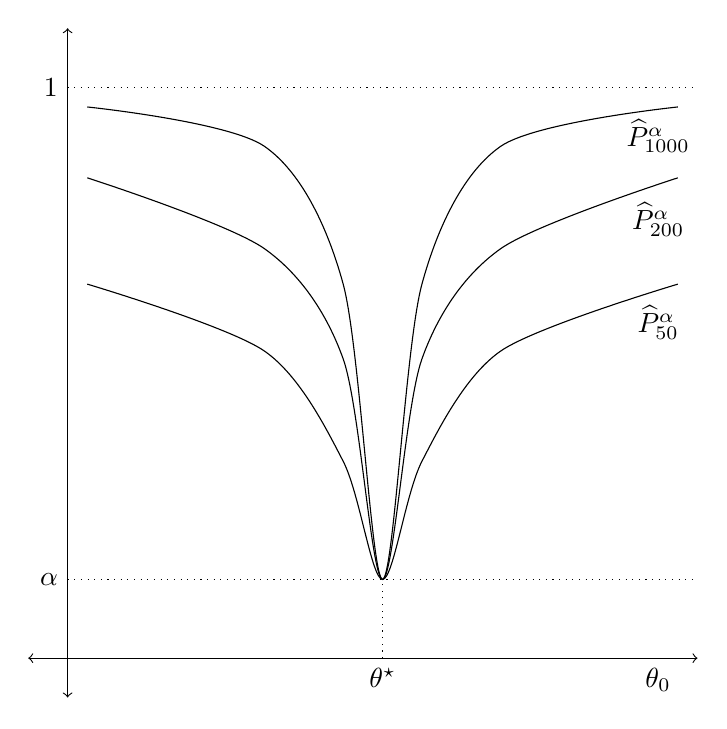
\begin{tikzpicture}[scale=1]
	
	% power envelopes
	\draw plot [smooth] coordinates {
	(0.25,7) 
	(2.5,6.5) 
	(3.5,4.75) 
	(4,1) 
	(4.5,4.75) 
	(5.5,6.5) 
	(7.75,7)};
	\draw plot [smooth] coordinates {
	(0.25,7*0.8+0.5) 
	(2.5,6.5*0.8) 
	(3.5,4.75*0.8) 
	(4,1) 
	(4.5,4.75*0.8) 
	(5.5,6.5*0.8) 
	(7.75,7*0.8+0.5)};
	\draw plot [smooth] coordinates {
	(0.25,7*0.6+0.55) 
	(2.5,6.5*0.6) 
	(3.5,4.75*0.6-0.35) 
	(4,1) 
	(4.5,4.75*0.6-0.35) 
	(5.5,6.5*0.6) 
	(7.75,7*0.6+0.55)};

	% power envelope labels
	\draw (7.5,6.97) node[anchor=north] {$\widehat{P}^\alpha_{1000}$};
	\draw (7.5,5.91) node[anchor=north] {$\widehat{P}^\alpha_{200}$};
	\draw (7.5,4.6) node[anchor=north] {$\widehat{P}^\alpha_{50}$};

	% axis labels
	%\draw (0,4.5) node[anchor=south,rotate=90] {$\text{rejection probability}$};	
	\draw (7.5,0) node[anchor=north] {$\theta_0$};

	% null
	\draw (4,0) node[anchor=north] {$\theta^\star$};	
	\draw[-,dotted] (4,0)--(4,1);
	%\draw[-] (4,-0.125)--(4,0.125);

	% size
	\draw (0,1) node[anchor=east] {$\alpha$};	
	\draw[-,dotted] (0,1)--(8,1);

	% probability 1
	\draw (0,7.25) node[anchor=east] {$1$};	
	\draw[-,dotted] (0,7.25)--(8,7.25);


	% axes
	\draw[<->] (-0.5,0) -- (8,0);
	\draw[<->] (0,-0.5) -- (0,8);
	%\fill (-0.007,-0.007) rectangle (0.007,0.007);

\end{tikzpicture}
	\caption{A family of local power envelopes for $\Theta \subseteq \R$ for a given $\alpha$ and $\theta^\star$. Power is high when $\theta_0$ is far from the null and $n$ is large.}
	\label{fig:power}
\end{figure}


Finally, the derivations in \cref{sec:hypothesis_testing:simple} showing that the LR, LM and Wald statistics are asymptotically equivalent (i.e. within $\op(1)$ of each other) apply with almost no changes to this new asymptotic environment. It follows that the LR and LM statistics are also noncentral-$\chi^2$-distributed, with the same noncentrality parameter, under local-DGP asymptotics. Their local power is therefore the same as that of the Wald test. Moreover, all of the results extend to (smooth) composite hypotheses: the trinity tests are still consistent, and their power can be approximated using a Pitman drift.



\pagebreak
%%%%%%%%%%%%%%%%%%%%%%%%%%%%%%%%%%%%%%%%%%%%%%%%%%%%%
%%%%%%%%%%%%%%%%%%%%%%%%%%%%%%%%%%%%%%%%%%%%%%%%%%%%%
\section{The generalised method of moments estimator}
\label{sec:GMM}
%%%%%%%%%%%%%%%%%%%%%%%%%%%%%%%%%%%%%%%%%%%%%%%%%%%%%
%%%%%%%%%%%%%%%%%%%%%%%%%%%%%%%%%%%%%%%%%%%%%%%%%%%%%

\emph{%Covered on 7 \& 9 Mar 2016.
Official reading: \textcite[][sec. 8.1.1 and 8.2.2]{Amemiya1985} and \textcite[][sec. 2.2.3, 2.5, 3.3 and 4.3]{NeweyMcfadden1994}.}



%%%%%%%%%%%%%%%%%%%%%%%%%%%%%
\subsection{Preliminaries}
\label{sec:GMM:preliminaries}
%%%%%%%%%%%%%%%%%%%%%%%%%%%%%

The generalised method of moments (GMM), introduced by \textcite{Hansen1982}, is a pretty general (haha) technique for estimation and inference that subsumes most parametric methods as special cases. It occupies an important place in the history of econometrics: before GMM, there were many disparate methods such as 2SLS, 3SLS and so on (as you can see by looking at \textcite{Amemiya1985}, which was written before GMM was introduced). GMM subsumed these classical methods as special cases.

We will treat the case in which the DGP $\{ y_i \}$ is iid. We have some (economic) model that gives us the moment conditions $\E\bigl( \widetilde{g}(y_1,\theta_0) \bigr) = 0$ for some known function $\widetilde{g} : \R^r \times \Theta \to \R^q$.%
	\footnote{A rather nice thing is that a lot of economic models give rise to moment conditions; Euler equations are one example. By contrast, it's very rare that a convincing economic model gives rise to a more restrictive statistical model such as a density (as required for maximum likelihood).}
Even if the model imposes additional structure on the data, GMM makes use only of these moment conditions.%
	\footnote{This is another advantage of GMM over e.g. ML. Suppose we have a model that gives us a likelihood from which we can derive moment conditions. If the likelihood is misspecified then our estimates will in general be inconsistent. But if the moment conditions hold (a much weaker condition in general), then GMM will give us consistent estimates.}
As usual we define the random functions $g_i : \Theta \to \R^q$ by $g_i(\omega)(\theta) \coloneqq \widetilde{g}(y_i(\omega),\theta)$, allowing us to write the moment conditions as $\E( g_1(\theta_0) ) = 0$.

So we have $q$ restrictions on the $k$-dimensional parameter $\theta_0$. We assume that $\theta_0$ is point-identified, meaning that $\theta_0$ is the unique solution in $\Theta$ to $\E( g_1(\theta) ) = 0$. A necessary condition for this is (obviously) $q \geq k$. The case $q > k$ is called overidentification; in the lingo, the model gives us overidentifying restrictions on $\theta_0$ in this case.%
	\footnote{Correspondingly, the case $q=k$ is called `exact identification'. Then we have enough restrictions to identify $\theta_0$, but no more.}
When the moment conditions are misspecified and $q>k$, it should be clear that $\E( g_1(\theta) ) = 0$ may not have a solution in $\Theta$. This indicates that we can formulate a specification test for the model by expoiting the overidentifying restrictions; we will work out the details in \cref{sec:GMM:specification} below.%
	\footnote{More generally, we could allow $\E( g_1(\theta) ) = 0$ to have multiple solutions, in which case we obtain partial identification. Another form of partially-identified GMM comes from replacing the moment equalities with moment \emph{in}equalities. The latter is currently a hot topic in econometric theory.}

Every parameteric estimator that we have mentioned so far is a GMM estimator for some choice of $\widetilde{g}$. In particular, any extremum estimator for which the FOC $\nabla Q_n\bigl( \widehat{\theta}_n \bigr) = 0$ holds is a GMM estimator. Since we're only covering GMM for the iid case, restrict attention to separable criterion functions, so that the FOC can be written
%
\begin{equation*}
	\sum_{i=1}^n \nabla q_i\bigl( \widehat{\theta}_n \bigr) = 0 .
\end{equation*}
%
Any such estimator is an exactly-identified ($q=k$) GMM estimator with $g_i = \nabla q_i$.

One example is the MLE, for which $g_i = \ell_i^1$. Another is the nonlinear least squares estimator, for which
%
\begin{equation*}
	\widetilde{g}((y,x),\theta) = \left( y - f(x,\theta) \right) x ,
\end{equation*}
%
and the moment condition is derived from the assumption $\E(y|x)=f(x,\theta_0)$. Yet another is the LAD estimator, where
%
\begin{equation*}
	\widetilde{g}((y,x),\theta) 
	= 2 \cdot \1\left( y \leq \theta \right) - 1 ,
\end{equation*}
%
and the moment condition is derived from the assumption that the median of the distribution of $y$ conditional on $x$ is $f(x,\theta)$.


When $q=k$ and $\widetilde{g}$ is well-behaved, the sample moment condition
%
\begin{equation*}
	n^{-1}\sum_{i=1}^n g_i(\theta) = 0
\end{equation*}
%
will have a unique solution. This value is called the method-of-moments estimator, and the sample moment condition is sometimes called an estimating equation in this context. But what can we do when $q>k$ or $\widetilde{g}$ is ill-behaved? One possibility is to throw away $q-k$ moment conditions and choose $\widetilde{\theta}_n$ to make $n^{-1} \sum_{i=1}^n g_i(\theta)$ as close as possible to zero in some metric (exactly equal to zero if $\widetilde{g}$ is well-behaved). More generally, we could set $k$ linear combinations of the sample moments as close as possible to zero (in some metric).

GMM is similar to the latter suggestion. We keep all $q$ moment conditions (instead of combining them into $k$ conditions), and we minimise their distance from zero in some metric. GMM uses a particular metric: a quadratic form in the sample moments. Writing $G_n \coloneqq n^{-1/2} \sum_{i=1}^n g_i$, the GMM objective function is
%
\begin{equation*}
	Q_n(\theta) 
	\coloneqq \frac{1}{2} G_n(\theta)^\trans W_n G_n(\theta)
	= \frac{1}{2} \left[ n^{-1/2} \sum_{i=1}^n g_i(\theta) \right]^\trans 
	W_n 
	\left[ n^{-1/2} \sum_{i=1}^n g_i(\theta) \right] .%
		\footnote{Most authors, including Joel, scale the objective function differently. I think that my scaling makes by far the most sense. First, having $n^{-1/2} \sum_{i=1}^n g_i(\theta)$ instead of $n^{-1} \sum_{i=1}^n g_i(\theta)$ or $\sum_{i=1}^n g_i(\theta)$ allows us to directly apply our results for extremum estimators. Second, the $1/2$ means that $Q_n$ is similar to the likelihood: the efficient GMM estimator will satisfy a generalised information matrix equality, and the LR stat will be $2\bigl( Q_n\bigl( \widetilde{\theta}_n \bigr) - Q_n\bigl( \widehat{\theta}_n \bigr) \bigr)$.}
\end{equation*}
%
The $q \times q$ weight matrix $W_n$ is allowed to be stochastic (a function of the data), but must satisfy $W_n = W + \op(1)$ for some symmetric, positive definite, nonstochastic $q \times q$ matrix $W$. The GMM estimator (for given moment conditions $\E( g_1(\theta_0) ) = 0$ and given weight matrix $W_n$) minimises $Q_n$. (So the GMM estimator is an extremum estimator.)



%%%%%%%%%%%%%%%%%%%%%%%%%%%
\subsection{Consistency}
\label{sec:GMM:consistency}
%%%%%%%%%%%%%%%%%%%%%%%%%%%

Conditions for consistency of GMM can be obtained (essentially) from our consistency results for extremum estimators (pp. \pageref{proposition:weak_consistency} and \pageref{proposition:strong_consistency}). We'll give primitive conditions for strong consistency in the iid case.

Assume that $\Theta$ is compact and that each $g_i$ is continuous (so that $Q_n$ is). Further assume that $\E\left( \sup_{\theta \in \Theta} \abs*{g_1(\theta)} \right) < \infty$. Then Jennrich's uniform SLLN (p. \pageref{theorem:Jennrich_uniform_SLLN}) applies, giving us
%
\begin{equation*}
	n^{-1/2} G_n 
	= n^{-1} \sum_{i=1}^n g_i
	\convas g
	\quad\text{uniformly over $\Theta$} ,
\end{equation*}
%
where $g : \Theta \to \R^q$ is the nonstochastic function $g(\theta) \coloneqq \E( g_1(\theta) )$. Hence
%
\begin{multline*}
	n^{-1} Q_n 
	= \frac{1}{2} \left[ n^{-1/2} G_n \right]^\trans W_n \left[ n^{-1/2} G_n \right]
	\\
	\convas \frac{1}{2} g^\trans W g \eqqcolon Q
	\quad\text{uniformly over $\Theta$} .
\end{multline*}
%
We assumed point identification, which says precisely that
%
\begin{equation*}
	g(\theta) = \E( g_1(\theta) ) = 0
	\quad\text{iff}\quad
	\theta = \theta_0 .
\end{equation*}
%
Hence $Q(\theta) = \frac{1}{2} g(\theta)^\trans W g(\theta) > 0$ for $\theta \neq \theta_0$ (remember that $W$ is positive definite) and $Q(\theta_0)=0$, so $Q$ is uniquely minimised at $\theta_0$.

We've now verified all of the conditions of our strong consistency result for extremum estimators (p. \pageref{proposition:strong_consistency}), so $\widehat{\theta}_n \convas \theta_0$.



%%%%%%%%%%%%%%%%%%%%%%%%%%%%%%%%%%%%
\subsection{Asymptotic normality}
\label{sec:GMM:asymptotic_normality}
%%%%%%%%%%%%%%%%%%%%%%%%%%%%%%%%%%%%

Unsurprisingly, we will appeal to our asymptotic normality result for extremum estimators (p. \pageref{proposition:asymptotic_normality}). Again we treat the iid case and give primitive conditions.

So maintain the assumptions we imposed to obtain strong consistency in the previous section, and assume that $\theta_0 \in \interior \Theta$. Further assume that each $g_i$ is twice continuously differentiable in a neighbourhood of $\theta_0$, so that $Q_n$ is too. Write $\DD g_i$ for the $q \times k$ first derivative, and $\DD^2 g_i$ for the $q \times k \times k$ second derivative. The latter is a three-dimensional array!


The derivatives of $Q_n$ are
%
\begin{align*}
	\nabla Q_n 
	={}& \left[ \DD G_n \right]^\trans W_n G_n
	\\
	\nabla^2 Q_n 
	={}& \left[ \DD G_n \right]^\trans W_n \left[ \DD G_n \right]
	+ \left[ \DD^2 G_n \right]^\trans W_n G_n .
\end{align*}
%
Don't forget that $\left[ \DD^2 G_n \right]^\trans W_n G_n$ is the product of a three-dimensional array with a matrix, yielding a matrix. My notation for this is not ideal (e.g. it doesn't tell the reader along what dimensions we're transposing the array), but it won't matter because this term is going to vanish. The first derivative of $G_n$ is of course
%
\begin{equation*}
	\DD G_n
	= n^{-1/2} \sum_{i=1}^n \DD g_i .
\end{equation*}


We'll want $n^{-1/2} \DD G_n$ to converge uniformly to $\DD g$, where
%
\begin{equation*}
	g(\theta) = \E(g_1(\theta))
\end{equation*}
%
as in the previous section. We already have that $\{ \DD g_i \}$ are iid and continuous and that $\Theta$ is compact, so we only have to add the assumption that $\E\left( \sup_{\theta \in \Theta} \abs*{\DD g_1(\theta)} \right) < \infty$. Jennrich's uniform SLLN (p. \pageref{theorem:Jennrich_uniform_SLLN}) then tells us that
%
\begin{equation*}
	n^{-1/2} \DD G_n(\theta)
	= n^{-1} \sum_{i=1}^n \DD g_i(\theta)
	\convas \DD g
	\quad\text{uniformly over $\Theta$} .
\end{equation*}
%
The uniform boundedness assumption on $g_1$ (that we used to derive consistency) is sufficient for the dominated convergence theorem, and hence for the interchanging of integration and differentiation. Therefore
%
\begin{equation*}
	\DD g(\theta)
	= \frac{\partial}{\partial \theta^\trans} \E(g_1(\theta)) 
	= \E\left( \frac{\dd}{\dd \theta^\trans} g_1(\theta) \right)
	= \E\left( \DD g_1(\theta) \right) .
\end{equation*} 
%
Good to know.

It follows by the dominated convergence theorem and independence that
%
\begin{align*}
	B
	={}& \lim_{n\to\infty}
	\E\left( n^{-1}
	[\nabla Q_n(\theta_0)] 
	[\nabla Q_n(\theta_0)]^\trans 
	\right)
	\\
	={}& \lim_{n\to\infty}
	\E\Big( 
	\left[ \left[ n^{-1/2} \DD G_n(\theta_0) \right]^\trans W_n G_n(\theta_0) \right] 
	\\
	&\quad\quad\quad\quad\quad\quad\times
	\left[ \left[ n^{-1/2} \DD G_n(\theta_0) \right]^\trans W_n G_n(\theta_0) \right]^\trans 
	\Big)
	\\
	={}& \lim_{n\to\infty}
	\E\left( 
	\left[ n^{-1/2} \DD G_n(\theta_0) \right]^\trans W_n G_n(\theta_0) 
	G_n(\theta_0)^\trans W_n^\trans \left[ n^{-1/2} \DD G_n(\theta_0) \right]
	\right)
	\\
	={}& \left[ \DD g(\theta_0) \right]^\trans W 
	\left\{
	\lim_{n\to\infty}
	\E\left( 
	G_n(\theta_0) G_n(\theta_0)^\trans
	\right)
	\right\}
	W \left[ \DD g(\theta_0) \right]
	\\
	={}& \left[ \DD g(\theta_0) \right]^\trans W 
	\left\{
	\lim_{n\to\infty}
	\E\left( 
	n^{-1} \sum_{i=1}^n \sum_{j=1}^n g_i(\theta_0) g_j(\theta_0)^\trans
	\right)
	\right\}
	W \left[ \DD g(\theta_0) \right]
	\\
	={}& \left[ \DD g(\theta_0) \right]^\trans W 
	\left\{
	\lim_{n\to\infty}
	\E\left( 
	n^{-1} \sum_{i=1}^n g_i(\theta_0) g_i(\theta_0)^\trans
	\right)
	\right\}
	W \left[ \DD g(\theta_0) \right]
	\\
	={}& \left[ \DD g(\theta_0) \right]^\trans W 
	\E\left( g_1(\theta_0) g_1(\theta_0)^\trans \right)
	W \left[ \DD g(\theta_0) \right] .
\end{align*}
%
(The penultimate equality holds by independence.)

Now let's do something similar for $\nabla^2 Q_n$. Add the Jennrich boundedness condition $\E\left( \sup_{\theta \in \Theta} \abs*{\DD^2 g_1(\theta)} \right) < \infty$ on the second derivative; then $n^{-1/2} \DD^2 G_n \convas \DD^2 g$ uniformly by Jennrich's uniform SLLN. So
%
\begin{align*}
	n^{-1} \nabla^2 Q_n 
	={}& \left[ n^{-1/2} \DD G_n \right]^\trans W_n \left[ n^{-1/2} \DD G_n \right]
	+ \left[ n^{-1/2} \DD^2 G_n \right]^\trans W_n \left[ n^{-1/2} G_n \right]
	\\
	\convas& \left[ \DD g \right]^\trans W \left[ \DD g \right]
	+ \left[ \DD^2 g \right]^\trans W g
	\quad\text{uniformly over $\Theta$} .
\end{align*}
%
So using $g(\theta_0)=0$, we have
%
\begin{align*}
	n^{-1} \nabla^2 Q_n(\theta_0)
	\convas& 
	\left[ \DD g(\theta_0) \right]^\trans W \left[ \DD g(\theta_0) \right]
	+ \left[ \DD^2 g(\theta_0) \right]^\trans W g(\theta_0) 
	\\
	={}& 
	\left[ \DD g(\theta_0) \right]^\trans W \left[ \DD g(\theta_0) \right] .
\end{align*}
%
Hence by the dominated convergence theorem,
%
\begin{equation*}
	A
	= \lim_{n\to\infty}
	\E\left( n^{-1} \nabla^2 Q_n(\theta_0) \right)
	= \left[ \DD g(\theta_0) \right]^\trans W \left[ \DD g(\theta_0) \right] .
\end{equation*}


The fact that
%
\begin{equation*}
	n^{-1} \nabla^2 Q_n 
	\convas \left[ \DD g \right]^\trans W \left[ \DD g \right] 
	+ \left[ \DD^2 g \right]^\trans W g
	\quad\text{uniformly over $\Theta$}
\end{equation*}
%
gives us that for any sequence $\{ \theta_n \}$ of random $k$-vectors with $\theta_n \convp \theta_0$, we have
%
\begin{equation*}
	n^{-1} \nabla^2 Q_n(\theta_n)
	\convp \left[ \DD g(\theta_0) \right]^\trans W \left[ \DD g(\theta_0) \right]
	= A .
\end{equation*}
%
You may recall that this is what assumption (3) in the asymptotic normality result for extremum estimators (p. \pageref{proposition:asymptotic_normality}) requires.

To verify the fourth and final hypothesis of the asymptotic normality result, first observe that
%
\begin{align*}
	n^{-1/2} \nabla Q_n(\theta_0) 
	={}& \left[ n^{-1/2} \DD G_n(\theta_0) \right]^\trans 
	W_n \left[ G_n(\theta_0) \right] 
	\\
	={}& \left[ \DD g(\theta_0) \right]^\trans 
	W \left[ n^{-1/2} \sum_{i=1}^n g_i(\theta_0) \right] + \op(1) .
\end{align*}
%
$\{ g_i(\theta_0) \}$ are iid with mean zero and variance $\E\left( g_1(\theta_0) g_1(\theta_0)^\trans \right)$, so by the multivariate Lindeberg--Lévy CLT and Slutsky's theorem,
%
\begin{align*}
	n^{-1/2} \nabla Q_n(\theta_0) 
	\convd& \left[ \DD g(\theta_0) \right]^\trans 
	W \mathcal{N}_q\left( 0, \E\left( g_1(\theta_0) g_1(\theta_0)^\trans \right) \right)
	\\
	\eqd& \mathcal{N}_q\left( 0, 
	\left[ \DD g(\theta_0) \right]^\trans W
	\E\left( g_1(\theta_0) g_1(\theta_0)^\trans \right)
	W \left[ \DD g(\theta_0) \right]
	\right)
	\\
	\eqd& \mathcal{N}_q\left( 0, B \right) .
\end{align*}


So we've satisfied all the conditions of our asymptotic normality result (p. \pageref{proposition:asymptotic_normality}). Hence
%
\begin{equation*}
	n^{1/2} \bigl( \widehat{\theta}_n - \theta_0 \bigr)
	\convd \mathcal{N}\left( 0, A^{-1} B A^{-1} \right) .
\end{equation*}
%
The asymptotic variance is the beast
%
\begin{multline*}
	A^{-1} B A^{-1}
	= 
	\left( \left[ \DD g(\theta_0) \right]^\trans W \left[ \DD g(\theta_0) \right] \right)^{-1}
	\left[ \DD g(\theta_0) \right]^\trans W 
	\E\left( g_1(\theta_0) g_1(\theta_0)^\trans \right)
	\\ \times
	W \left[ \DD g(\theta_0) \right]
	\left( \left[ \DD g(\theta_0) \right]^\trans W \left[ \DD g(\theta_0) \right] \right)^{-1} .
\end{multline*}



%%%%%%%%%%%%%%%%%%%%%%%%%%%%%%%%%%%%%
\subsection{Asymptotic efficiency}
\label{sec:GMM:asymptotic_efficiency}
%%%%%%%%%%%%%%%%%%%%%%%%%%%%%%%%%%%%%

In general, there's no reason to think that the GMM estimator is asymptotically efficient within (say) the class of consistent and asymptotically normal estimators. For if the moment conditions are uninformative then there's no way to obtain a low-variance estimator.

Instead, we fix the moment conditions and search for the asymptotically most efficient estimator that uses only this information. Since the only parameter in GMM estimation that can be varied is the weight matrix $W_n$, the theory of efficient GMM amounts to the theory of how to optimally choose $W_n$. Of course only the probability limit $W$ of $\{ W_n \}$ matters, so really we're choosing $W$.

It turns out that an (infeasible) optimal choice of weight matrix is $W = \E\left( g_1(\theta_0) g_1(\theta_0)^\trans \right)^{-1}$. (We won't show this, but it's straightforward matrix algebra.) So the asymptotic variance of an efficient GMM estimator is
%
\begin{align*}
	A^{-1} B A^{-1}
	={}& 
	\left( \left[ \DD g(\theta_0) \right]^\trans W \left[ \DD g(\theta_0) \right] \right)^{-1}
	\left[ \DD g(\theta_0) \right]^\trans W 
	W^{-1}
	\\ 
	&\quad\quad\quad\quad\quad\times
	W \left[ \DD g(\theta_0) \right]
	\left( \left[ \DD g(\theta_0) \right]^\trans W \left[ \DD g(\theta_0) \right] \right)^{-1} .
	\\
	={}& \left( \left[ \DD g(\theta_0) \right]^\trans 
	W \left[ \DD g(\theta_0) \right] \right)^{-1}
	\\
	={}& \left( \left[ \DD g(\theta_0) \right]^\trans 
	\E\left( g_1(\theta_0) g_1(\theta_0)^\trans \right)^{-1} 
	\left[ \DD g(\theta_0) \right] \right)^{-1}	
	\\
	={}& A^{-1} = B^{-1} .
\end{align*}
%
There's a close analogy with the efficiency of (correctly-specified) MLE here. The efficient choice of weight matrix (resp. density) causes a bunch of cancellations in the asymptotic variance, leaving us with $A^{-1}$. (It's $A$ rather than $-A$ because we're minimising $Q_n$, so $\nabla^2 Q_n$ is \emph{positive} definite here.) Moreover, we obtain $A=B$, a generalisation of the information matrix equality.%
	\footnote{If you remember how we made use of the information matrix equality to derive the asymptotic distribution of the LR statistic, then you should realise that the LR-type statistic $2\bigl( Q_n\bigl( \widetilde{\theta}_n \bigr) - Q_n\bigl( \widehat{\theta}_n \bigr) \bigr)$ will be asymptotically $\chi^2$ in the efficient GMM setting just as in correctly specified MLE.}
Clearly $B^{-1}$ is the lower bound on the variance of any GMM estimator using these moment conditions, analogous to the Cramér--Rao bound.


So far we only have an infeasible procedure, since it requires knowledge of $\E\left( g_1(\theta_0) g_1(\theta_0)^\trans \right)^{-1}$. But provided we can consistently estimate the latter, we can obtain a feasible estimator. The standard way of doing this (proposed by \textcite{Hansen1982}) is called two-step GMM. First pick some arbitrary weight matrix $W_n$,%
	\footnote{There's some evidence on what is and is not a good idea for a first-step weight matrix. The identity is very bad; the 2SLS weight matrix is pretty good. (The 2SLS weight matrix is consistent for $B^{-1}$ in the linear homoskedastic case.)}
and obtain the GMM estimate $\widetilde{\theta}_n$. Define the $\Theta \to \R^{q \times q}$ function
%
\begin{equation*}
	\widehat{W}_n \coloneqq \left( n^{-1} \sum_{i=1}^n g_i g_i^\trans \right)^+ ,
\end{equation*}
%
and estimate $\E\left( g_1(\theta_0) g_1(\theta_0)^\trans \right)^{-1}$ by $\widehat{W}_n\bigl( \widetilde{\theta}_n \bigr)$. This estimator is obviously consistent under the maintained assumptions. Now do GMM again using the estimated optimal weight matrix to obtain the two-step GMM estimate $\widehat{\theta}_n$. Since $\widehat{W}_n$ is asymptotically equivalent to $\E\left( g_1(\theta_0) g_1(\theta_0)^\trans \right)^{-1}$, $\widehat{\theta}_n$ is asymptotically equivalent to the infeasible efficient GMM estimator above. The two-step GMM estimator $\widehat{\theta}_n$ is therefore asymptotically efficient within the class of GMM estimators that use these moment conditions.

There are serious finite-sample problems with the two-step procedure. The intermediate step of estimating $\E\left( g_1(\theta_0) g_1(\theta_0)^\trans \right)^{-1}$ lowers the asymptotic variance, but at the cost of introducing an additional source of noise into the estimator. Worse, the noise in estimating the optimal weight matrix is generally correlated with the noise in the sample moments $G_n$, which introduces bias into the two-step GMM estimator. In Monte Carlo studies, this bias is quite severe for nonlinear DGPs, even in large samples.

There are two obvious ways of dealing with finite-sample bias. On the one hand, we could just eschew two-step GMM in favour of one-step GMM, which is asymptotically less efficient but allows for more reliable inference. (And may be more efficient in a finite sample!) On the other hand, we could incorporate finite-sample corrections to our estimates. Many have been proposed, and some of them are quite helpful.

Another solution is to use a one-step procedure that nevertheless delivers an estimator that is asymptotically equivalent to the infeasible efficient GMM estimator. The continuously-updated (CUE) GMM estimator maximises
%
\begin{equation*}
	G_n(\theta)^\trans \widehat{W}_n(\theta) G_n(\theta) ,
\end{equation*}
%
obviating the need for a second step. And it turns out (perhaps unsurprisingly) to be asymptotically equivalent to the infeasible efficient GMM estimator that uses weight matrix $\E\left( g_1(\theta_0) g_1(\theta_0)^\trans \right)^{-1}$. The lack of an initial step turns out to make a big difference: the Monte Carlo evidence is that the finite-sample behaviour of the CUE GMM estimator is much better than that of two-step GMM. Unfortunately, obtaining the CUE GMM estimator is in general a pretty hard problem: even when $\widetilde{g}$ is linear, it is a nonlinear optimisation problem.

Yet another one-step method that is asymptotically equivalent to efficient GMM is the empirical likelihood (EL) estimator. The EL estimator is the first part of the argmax in the problem
%
\begin{equation*}
	\max_{ (\theta,p) \in \Theta \times (0,1)^n }
	\sum_{i=1}^n \ln(p_i)
	\quad\text{s.t.}\quad
	n^{-1} \sum_{i=1}^n g_i(\theta) = 0
	\quad\text{and}\quad \sum_{i=1}^n p_i = 1 .
\end{equation*}
%
Again, the asymptotics are the same as for efficient GMM, but the finite-sample properties are much better. And again, this estimator is computationally troublesome, as we're now maximising over $k+n$ variables with an additional constraint. There's a broader class of estimators called generalised empirical likelihood (GEL) estimators which share these good finite-sample properties. We won't delve into (G)EL estimation here; see \textcite{Imbens2002} for a nice intro-level survey.



%%%%%%%%%%%%%%%%%%%%%%%%%%%%%%%%%%%%%%%%%%%%%
\subsection{The \texorpdfstring{$J$}{J} test}
\label{sec:GMM:specification}
%%%%%%%%%%%%%%%%%%%%%%%%%%%%%%%%%%%%%

Recall that we defined $\theta_0$ to be the unique solution to the population moment condition $\E( g_1(\theta_0) ) = 0$. So we know that the model is misspecified (in the precise sense that the moment conditions are inconsistent with each other) if $\E( g_1(\theta) ) = 0$ has no solution in $\Theta$.

When $q=k$ (exact identification), provided $g_1$ is moderately well-behaved, our GMM procedure will force all $q$ sample moment conditions to hold. Intuitively, whenever a moment condition fails, we will have a degree of freedom (a parameter whose estimate we have not yet determined) that we can play with until the last sample moment is satisfied.

But consider the overidentified case $q>k$. Intuitively, we can only force $k$ of the sample moment conditions to hold, leaving another $q-k$ free to do as they please. If the model is correctly specified (the moment conditions hold in the population) then the additional moments should be close to zero. This provides the basis for a specification test, i.e. a test of the null hypothesis that the model is correctly specified.%
	\footnote{The information matrix test is another specification test. The $J$ test is conceptually distinct from the information matrix test, however. Given that we derived a generalised information matrix equality for efficient GMM, we could formulate an information matrix test for GMM if desired.}
The test is sometimes called the Hansen $J$ test, or else simply the test of overidentifying restrictions.


To that end, consider the LR-type statistic
%
\begin{equation*}
	J_n
	\coloneqq 2 Q_n\bigl( \widehat{\theta}_n \bigr) 
	= G_n\bigl( \widehat{\theta}_n \bigr)^\trans 
	W_n G_n\bigl( \widehat{\theta}_n \bigr) .
\end{equation*}
%
Though it has the flavour of an LR statistic, note that we are not testing the null hypothesis that the true parameter satisfies some restriction. Instead, our null is that $Q_n(\theta_0)$ is $\op(1)$, meaning that all the moment conditions are satisfied at the truth.


To derive the asymptotic distribution under the null, begin with a mean-value expansion:
%
\begin{align*}
	G_n\bigl( \widehat{\theta}_n \bigr)
	={}& G_n( \theta_0 )
	+ \left[ n^{-1/2} \DD G_n\bigl( \widetilde{\theta}_n \bigr) \right]
	\left[ n^{1/2} \bigl( \widehat{\theta}_n - \theta_0 \bigr) \right]
	\\
	={}& G_n( \theta_0 )
	+ \left[ \DD g( \theta_0 ) \right] 
	\left[ n^{1/2} \bigl( \widehat{\theta}_n - \theta_0 \bigr) \right]
	+ \op(1)
\end{align*}
%
where $\widetilde{\theta}_n$ is the mean value. Recall from our proof of asymptotic normality for extremum estimators (p. \pageref{proposition:asymptotic_normality}) that
%
\begin{align*}
	n^{1/2} \bigl( \widehat{\theta}_n - \theta_0 \bigr)
	={}& - \left[ n^{-1} \nabla^2 Q_n\bigl( \widetilde{\theta}_n \bigr) \right]^+
	\left[ n^{-1/2} \nabla Q_n\left( \theta_0 \right) \right] 
	\\
	={}& - \left( \left[ n^{-1/2} \DD G_n\bigl( \widetilde{\theta}_n \bigr) \right]^\trans 
	W_n \left[ n^{-1/2} \DD G_n\bigl( \widetilde{\theta}_n \bigr) \right] \right)^+
	\\
	&\quad\quad\quad\times
	\left( \left[ n^{-1/2} \DD G_n(\theta_0) \right]^\trans W_n G_n(\theta_0) \right)
	\\
	={}& - \left( \left[ \DD g(\theta_0) \right]^\trans 
	W \left[ \DD g(\theta_0) \right] \right)^{-1}
	\left[ \DD g(\theta_0) \right]^\trans W G_n(\theta_0)
	+ \op(1)
\end{align*}
%
where $\widetilde{\theta}_n$ is also a mean value. So
%
\begin{align*}
	G_n\bigl( \widehat{\theta}_n \bigr)
	={}& G_n( \theta_0 )
	- \left[ \DD g( \theta_0 ) \right] 
	\left( \left[ \DD g(\theta_0) \right]^\trans 
	W \left[ \DD g(\theta_0) \right] \right)^{-1}
	\\
	&\quad\quad\quad\quad\quad\times
	\left[ \DD g(\theta_0) \right]^\trans W G_n(\theta_0)
	+ \op(1) .
\end{align*}


You may be tempted to use the matrix algebra result in \cref{eq:convenient_fact_raw} (p. \pageref{eq:convenient_fact_raw}) here to write
%
\begin{equation*}
	\left[ \DD g( \theta_0 ) \right] 
	\left( \left[ \DD g(\theta_0) \right]^\trans 
	W \left[ \DD g(\theta_0) \right] \right)^{-1}
	\left[ \DD g(\theta_0) \right]^\trans
	= W^{-1} ,
\end{equation*}
%
but this is a mistake! The reason is that $\left[ \DD g( \theta_0 ) \right] \left[ \DD g( \theta_0 ) \right]^\trans$ must have full rank in order for this identity to hold. But since $\DD g( \theta_0 )$ is $q \times k$ and $q > k$ by assumption, $\left[ \DD g( \theta_0 ) \right] \left[ \DD g( \theta_0 ) \right]^\trans$ can have rank at most $k$!


Instead, premultiply $G_n\bigl( \widehat{\theta}_n \bigr)$ by $W^{1/2}$:
%
\begin{multline*}
	W^{1/2} G_n\bigl( \widehat{\theta}_n \bigr)
	\\
	\begin{aligned}
		={}& W^{1/2} G_n( \theta_0 )
		- W^{1/2} \left[ \DD g( \theta_0 ) \right] 
		\left( \left[ \DD g(\theta_0) \right]^\trans 
		W \left[ \DD g(\theta_0) \right] \right)^{-1}
		\\
		&\quad\quad\quad\quad\quad\times
		\left[ \DD g(\theta_0) \right]^\trans W G_n(\theta_0)
		+ \op(1) 
		\\
		={}& \bigl\{ I
		- W^{1/2} \left[ \DD g( \theta_0 ) \right] 
		\left( \left[ \DD g(\theta_0) \right]^\trans 
		W \left[ \DD g(\theta_0) \right] \right)^{-1}
		\left[ \DD g(\theta_0) \right]^\trans W^{1/2} \bigr\}
		\\
		&\quad\quad\quad\quad\quad\times
		W^{1/2} G_n( \theta_0 )	+ \op(1) 
		\\
		={}& M W^{1/2} G_n( \theta_0 ) + \op(1) ,
	\end{aligned}
\end{multline*}
%
where
%
\begin{equation*}
	M \coloneqq I
	- W^{1/2} \left[ \DD g( \theta_0 ) \right] 
	\left( \left[ \DD g(\theta_0) \right]^\trans 
	W \left[ \DD g(\theta_0) \right] \right)^{-1}
	\left[ \DD g(\theta_0) \right]^\trans W^{1/2}
\end{equation*}
%
$M$ is symmetric (obvious) and idempotent (trivial to verify, just compute $MM$ and cancel terms to recover $M$).%
	\footnote{A square matrix $M$ is idempotent iff $MM=M$.}


So the test statistic is
%
\begin{align*}
	J_n
	={}& \left[ W_n^{1/2} G_n\bigl( \widehat{\theta}_n \bigr) \right]^\trans 
	\left[ W_n^{1/2} G_n\bigl( \widehat{\theta}_n \bigr) \right] 
	\\
	={}& \left[ W^{1/2} G_n\bigl( \widehat{\theta}_n \bigr) \right]^\trans 
	\left[ W^{1/2} G_n\bigl( \widehat{\theta}_n \bigr) \right] 
	+ \op(1)
	\\
	={}& \left[ M W^{1/2} G_n( \theta_0 ) \right]^\trans 
	\left[ M W^{1/2} G_n( \theta_0 ) \right] 
	+ \op(1)
	\\
	={}& \left[ W^{1/2} G_n( \theta_0 ) \right]^\trans 
	M^\trans M
	\left[ W^{1/2} G_n( \theta_0 ) \right] 
	+ \op(1) 
	\\
	={}& \left[ W^{1/2} G_n( \theta_0 ) \right]^\trans 
	M
	\left[ W^{1/2} G_n( \theta_0 ) \right] 
	+ \op(1) .
\end{align*}
%
It's immediate by the Lindeberg--Lévy CLT that 
%
\begin{equation*}
	G_n( \theta_0 ) \convd 
	\mathcal{N}_q\left( 0, \E\left( g_1(\theta_0) g_1(\theta_0)^\trans \right) \right) .
\end{equation*}
%
Now suppose (this is important!) that we choose the weight matrix optimally: $W = \E\left( g_1(\theta_0) g_1(\theta_0)^\trans \right)^{-1}$. Then we obtain
%
\begin{equation*}
	W^{1/2} G_n( \theta_0 ) 
	\convd \mathcal{N}_q\left( 0, W^{1/2} W^{-1} W^{1/2} \right) 
	\eqd \mathcal{N}_q\left( 0, I \right) .
\end{equation*}
%
It then follows by Slutsky's theorem that
%
\begin{align*}
	J_n
	={}& \left[ W^{1/2} G_n( \theta_0 ) \right]^\trans 
	M
	\left[ W^{1/2} G_n( \theta_0 ) \right] 
	+ \op(1)
	\\
	\convd& 
	\left[ \mathcal{N}_q\left( 0, I \right) \right]^\trans 
	M
	\left[ \mathcal{N}_q\left( 0, I \right) \right] .
\end{align*}


Now here's a fact for you: for $\xi \sim \mathcal{N}_q\left( 0, I \right)$ and any symmetric and idempotent $q \times q$ matrix $M$,
%
\begin{equation*}
	\xi^\trans M \xi \sim \chi^2\left( \rank M \right) .
\end{equation*}
%
To see why, eigen-decompose $M$ as $P^\trans \Lambda P$, where $\Lambda$ is a diagonal matrix with the eigenvalues of $M$ on the diagonal and $P$ contains the eigenvectors. Wlog, arrange the rows so that the zero eigenvalues are last. Then
%
\begin{equation*}
	\xi^\trans M \xi 
	= \left( P \xi \right)^\trans 
	\Lambda
	\left( P \xi \right)
	= \sum_{j=1}^q \lambda_j \left( (P \xi)_j \right)^2
	= \sum_{j=1}^{\rank M} \lambda_j \left( (P \xi)_j \right)^2 .
\end{equation*}
%
Since $M$ is idempotent, all its eigenvalues are either zero or unity, so
%
\begin{equation*}
	\xi^\trans M \xi 
	= \sum_{j=1}^{\rank M} \left( (P \xi)_j \right)^2 .
\end{equation*}
%
Since $P \xi$ is a linear combination of normals, it is normally distributed. Since the eigenvectors are orthogonal and the components of $\xi$ are independent, the components of $P\xi$ are independent. Moreover
%
\begin{equation*}
	\Var( (P\xi)_j ) 
	= P_{j,\cdot} \Var(\xi_j) P_{j,\cdot}^\trans 
	= P_{j,\cdot} P_{j,\cdot}^\trans 
	= 1
\end{equation*}
%
since $P$ is an orthogonal matrix. So we've shown that $\bigl\{ (P \xi)_j \bigr\}_{j=1}^{\rank M}$ are independent standard-normal-distributed random variables. Therefore 
%
\begin{equation*}
	\xi^\trans M \xi 
	= \sum_{j=1}^{\rank M} \left( (P \xi)_j \right)^2
	\sim \chi^2\left( \rank M \right) .
\end{equation*}


So let's compute the rank of our matrix
%
\begin{equation*}
	M = I
	- W^{1/2} \left[ \DD g( \theta_0 ) \right] 
	\left( \left[ \DD g(\theta_0) \right]^\trans 
	W \left[ \DD g(\theta_0) \right] \right)^{-1}
	\left[ \DD g(\theta_0) \right]^\trans W^{1/2} .
\end{equation*}
%
Using the fact that the rank and trace of an idempotent matrix are equal, and writing $I_m$ for an $m \times m$ identity matrix to make the dimensions explicit,
%
\begin{multline*}
	\rank M
	\\
	\begin{aligned}
	={}& \tr M
	\\
	={}& \tr I_q
	- \tr W^{1/2} \left[ \DD g( \theta_0 ) \right] 
	\left( \left[ \DD g(\theta_0) \right]^\trans 
	W \left[ \DD g(\theta_0) \right] \right)^{-1}
	\left[ \DD g(\theta_0) \right]^\trans W^{1/2}
	\\
	={}& \tr I_q
	- \tr 
	\left( \left[ \DD g(\theta_0) \right]^\trans 
	W \left[ \DD g(\theta_0) \right] \right)^{-1}
	\left[ \DD g(\theta_0) \right]^\trans W^{1/2}
	W^{1/2} \left[ \DD g( \theta_0 ) \right] 
	\\
	={}& \tr I_q
	- \tr I_k
	\\
	={}& q - k .
	\end{aligned}
\end{multline*}
%
So using our fun fact, we obtain
%
\begin{equation*}
	J_n
	\convd 
	\left[ \mathcal{N}_q\left( 0, I \right) \right]^\trans 
	M
	\left[ \mathcal{N}_q\left( 0, I \right) \right] 
	\eqd \chi^2\left( \rank M \right) 
	\eqd \chi^2\left( q-k \right) .
\end{equation*}


That was the distribution under the null (correct specification). It's pretty clear that the test is consistent, for the same sort of reason as the trinity tests in \cref{sec:hypothesis_testing} were. We can also construct a Pitman drift such that the asymptotic distribution under local-DGP asymptotics is noncentral $\chi^2$.



%______________________________________________________________________________




%       _                               _ _               
%      / \   _ __  _ __   ___ _ __   __| (_) ___ ___  ___ 
%     / _ \ | '_ \| '_ \ / _ \ '_ \ / _` | |/ __/ _ \/ __|
%    / ___ \| |_) | |_) |  __/ | | | (_| | | (_|  __/\__ \
%   /_/   \_\ .__/| .__/ \___|_| |_|\__,_|_|\___\___||___/
%           |_|   |_|                                     


%\pagebreak
%\begin{appendices}



%\end{appendices}



%______________________________________________________________________________




%    ____  _ _     _ _                             _           
%   | __ )(_) |__ | (_) ___   __ _ _ __ __ _ _ __ | |__  _   _ 
%   |  _ \| | '_ \| | |/ _ \ / _` | '__/ _` | '_ \| '_ \| | | |
%   | |_) | | |_) | | | (_) | (_| | | | (_| | |_) | | | | |_| |
%   |____/|_|_.__/|_|_|\___/ \__, |_|  \__,_| .__/|_| |_|\__, |
%                            |___/          |_|          |___/ 


\pagebreak
\printbibliography[heading=bibintoc]



%______________________________________________________________________________




\end{document}